% -*- mode: latex; -*- mustache tags:  
\documentclass[10pt,twoside,english]{_support/latex/sbabook/sbabook}
\let\wholebook=\relax

\usepackage{import}
\subimport{_support/latex/}{common.tex}

%=================================================================
% Debug packages for page layout and overfull lines
% Remove the showtrims document option before printing
\ifshowtrims
  \usepackage{showframe}
  \usepackage[color=magenta,width=5mm]{_support/latex/overcolored}
\fi


% =================================================================
\title{Learning Object-Oriented Programming, Design and TDD with Pharo}
\author{Stéphane Ducasse}
\series{The Pharo TextBook Collection}

\hypersetup{
  pdftitle = {Learning Object-Oriented Programming, Design and TDD with Pharo},
  pdfauthor = {Stéphane Ducasse},
  pdfkeywords = {Introduction, programming, design, testing, Pharo, Smalltalk}
}


% =================================================================
\begin{document}

% Title page and colophon on verso
\maketitle
\pagestyle{titlingpage}
\thispagestyle{titlingpage} % \pagestyle does not work on the first one…

\cleartoverso
{\small

  Copyright 2017 by Stéphane Ducasse.

  The contents of this book are protected under the Creative Commons
  Attribution-ShareAlike 3.0 Unported license.

  You are \textbf{free}:
  \begin{itemize}
  \item to \textbf{Share}: to copy, distribute and transmit the work,
  \item to \textbf{Remix}: to adapt the work,
  \end{itemize}

  Under the following conditions:
  \begin{description}
  \item[Attribution.] You must attribute the work in the manner specified by the
    author or licensor (but not in any way that suggests that they endorse you
    or your use of the work).
  \item[Share Alike.] If you alter, transform, or build upon this work, you may
    distribute the resulting work only under the same, similar or a compatible
    license.
  \end{description}

  For any reuse or distribution, you must make clear to others the
  license terms of this work. The best way to do this is with a link to
  this web page: \\
  \url{http://creativecommons.org/licenses/by-sa/3.0/}

  Any of the above conditions can be waived if you get permission from
  the copyright holder. Nothing in this license impairs or restricts the
  author's moral rights.

  \begin{center}
    
\includegraphics[width=0.2\textwidth]{_support/latex/sbabook/CreativeCommons-BY-SA.pdf}
  \end{center}

  Your fair dealing and other rights are in no way affected by the
  above. This is a human-readable summary of the Legal Code (the full
  license): \\
  \url{http://creativecommons.org/licenses/by-sa/3.0/legalcode}

  \vfill

  % Publication info would go here (publisher, ISBN, cover design…)
  Layout and typography based on the \textcode{sbabook} \LaTeX{} class by Damien
  Pollet.
}


\frontmatter
\pagestyle{plain}

\tableofcontents*
\clearpage\listoffigures

\mainmatter

\chapter{About this book }\label{ch:about}\section{A word of presentation}
I started to write this book back in 1998 when I wrote around 900 pages in preparation for \textit{Learning Programming with Robots}
(Apparently, I needed to write to understand what I wanted to explain and how). From this I extracted \textit{Learning Programming with Robots}, which was a book to teach simple concepts such as variables, loops, procedures and to help people teach kids how to program. My original objective was to write a second volume to teach object-oriented programming. But while this first volume was a success, I got really frustrated because to be understandable by everyone I had to remove what I like: object-oriented programming and good object-oriented design. 

At that time, I met Harald Wertz, who gave me really nice ideas and pointers such as L-systems, then asked why I focused on procedural thinking and suggested that I should teach object-oriented programming instead. And he was right. This remark was like a bee in my bonnet for more than ten years.
In fact, it was my original objective but I was exhausted after my first attempt and I had to focus on my academic life.

Now, nearly fifteen years later, I'm ready to write a book to start with object-oriented programming. In fact, I rewrote everything I got from that time. 
I hope that you will enjoy it as much as I did — even if, for me, writing a book is a really long and daunting task because I want to make it great.
I plan to write another volume on patterns of design that will extend this book.
\section{Structure of the book}
While writing this book, I faced a challenge to find the correct level of difficulty.
To solve this problem, I structured the book either into key chapters on basic concepts, or into projects on more advanced topics.
The projects are little tutorials or more realistic examples, with step by step explanations; you can skip over them and come back to read them whenever you feel like it.
I also propose various paths through the book with different levels of reading; however, many of the \textit{simpler} chapters also contain design remarks.


\begin{figure}

\begin{center}
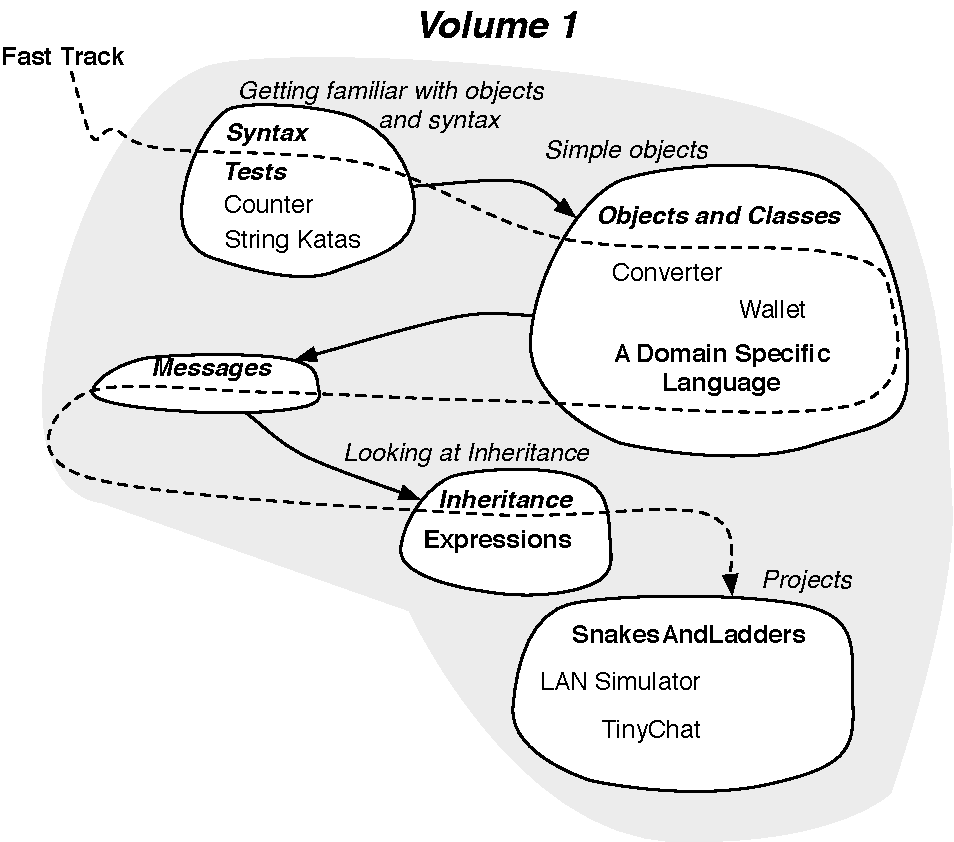
\includegraphics[width=1.0\textwidth]{/Users/ducasse/Workspace/FirstCircle/MyBooks/Bk-Writing/PharoBooks/LearningOOPWithPharoTrans/_result/pdf/Chapters/Introduction/figures/MapVolume1.pdf}\caption{Reading maps.\label{fgmap}}\end{center}
\end{figure}

\subsection{Fast track}
The following chapters contain more conceptual information:

In the volume 1:

\begin{itemize}
\item Glimpse of the syntax
\item Tests, tests and tests
\item Objects and classes
\item Revisiting objects and classes
\item Domain specific language
\item Inheritance and expressions
\item Sending messages
\item Snakes and ladders
\end{itemize}

The other chapters are more exercise and practical. For example, with TinyChat, you will have fun with a web server written in the single page of code. You will find the solutions of the exercises in a separate pdf available on the book web site at \url{http://books.pharo.org} and the associated github repository \url{https://github.com/SquareBracketAssociates/LearningOOPWithPharo}.
\section{What you will learn}
I would like to present the concepts that I want to teach you and that hopefully you should acquire. What is key to understand is that I will focus on the \textit{key} conceptual elements. It is easy for me because I will not explain OOP/D in general but within the context of Pharo and Pharo is the essence of Object-Oriented programming since its object model is minimal but it covers the key and essential aspect of OOP. For example, we will not present method modifiers, types, or overloading (which is a bad concept).

We will focus on object-oriented \textit{programming} concepts:

\begin{itemize}
\item Objects / Classes 
\item Messages / Methods
\item \textcode{self} and its semantics
\item Inheritance
\item \textcode{super} and its semantics
\end{itemize}

…and on object-oriented \textit{design} concepts:

\begin{itemize}
\item Class responsibility collaboration
\item Delegation
\item Message sends are choice
\item Message sends are plans for reuse
\item The \symbol{34}Don't ask, tell\symbol{34} Principle
\item Tests are your life insurance
\item Polymorphism
\end{itemize}

In addition, we will also present 

\begin{itemize}
\item Tests
\item Software refactorings
\end{itemize}
\subsection{Growing software}
Often books present a problem and its solution. Now for non-trivial problems, the solution does not fall from the sky or get developed in one stroke, but it is the constant evolution of a first solution that evolves over time. Such an evolution is often difficult and tedious because the developer jumps from one stable state to a situation where his code may not work anymore. This is where Test Driven Design and refactorings really help.
Test Driven Design helps focusing on new features and captures them as executable entities: tests. Refactorings help by transforming code without breaking its invariants.
Note that tests do not forbid to break code, they help identifying when previous invariants or constraints got violated. Sometimes violated tests identify a bug, but they may be broken just because the requirements changed and that the tests should be updated. 
In this book, I wanted to see how software grows in little steps. This is what I do frequently during my coding sessions, and I think that this is important, to cover the hidden paths in software creation.
\subsection{Syntax, blocks and iterators}
Since we need a language to express our programs, we will teach you the syntax of Pharo. In particular, we will use some simple chapters to get you started. 

Now in a nutshell, you should know that the Pharo syntax

\begin{itemize}
\item fits in one postcard and
\item is based on objects, messages and closures.
\end{itemize}

Note that closures are not a recent addition to the language but a central cornerstone. Closures are the foundation for conditionals and loops.
They enable this 'messages all over the place' syntax as well as really powerful iterators.
\section{Typographic conventions}
Pharo expressions or code snippets are represented either in the text as \textcode{'Hello'} and \textcode{'Hello' reversed}, or for more substantial snippets, as follows:

\begin{displaycode}{plain}
'Hello'
\end{displaycode}

When we want to show the result of evaluating an expression, we show the result after three chevrons \textcode{\textgreater{}\textgreater{}\textgreater{}} on the next line, like so:

\begin{displaycode}{plain}
'Hello' reversed
>>> 'olleH'
\end{displaycode}

Whenever we feel the text makes a point that is important or technical enough to be highlighted, we will do so with a thick bar:

\begin{important}
This is a point that is worth drawing some more attention.
\end{important}

Finally, the coffee cups highlight some points to take away and serve as a concise summary of the sections:

\begin{coffee}
If you skim through a section, take a few seconds to check for coffee cups!
\end{coffee}
\section{Videos }
While reading this book, you can also use some of the videos produced for the Pharo mooc. All the videos are available at \url{http://mooc.pharo.org}.
I strongly suggest to watch the videos explaining how to use and interact with the environment. 
\section{Thanks}
I would like to thanks Morgane Pigny, Anne Etien, Quentin Ducasse, Sven van Caekenberghe, Hayatou Oumarou, Kateryna Aloshkina, Ricardo Pacheco, Olivier Auverlot, Mariette Biernacki, Herby Vojcik, Denis Kudriashov, Holger Freyther, Dimitris Chloupis, Amal Noussi, Ren\'{e} Paul Mages, Hannes Hirsel, Lorenzo Solano Martinez for their great feedback.
Alexandre Bergel for his examples on messages. Olivier Auverlot for his constant enthousiam and for TinyChat. Guillermo Polito for the idea of file and directory example. Damien Pollet for this great template and the new LAN implementation and the numerous makefile implementation and Pillar help.

\part{Getting in touch with Pharo}\chapter{Pharo syntax in a nutshell}\label{cha:syntax}
In this chapter, we start on a simple path to get you to understand the most important parts of the Pharo syntax: \textit{messages}, \textit{blocks} and \textit{methods}.
This chapter is freely inspired from Sven van Caeckenberghe's gentle syntax introduction, and I thank him for giving me the permission to reuse his ideas.

In Pharo, everything is an \textit{object} and computation happens by sending \textit{messages} to objects.
Objects are created by sending messages to particular objects named \textit{classes}, which define the structure and behavior of the objects they create, also known as their instances.
\section{Simplicity and elegance of messages}
Messages are central to computation in Pharo.
While their syntax is quite minimalist, it is very expressive and structures most of the language.

There are three kinds of messages: unary, binary, and keyword-based.
\subsection{Sending a message \& the receiver}
Let’s first look at an example of sending a message to an object:

\begin{displaycode}{plain}
'hello' reversed
\end{displaycode}

What this means is that the message \textcode{reversed} is sent to the literal string \textcode{'hello'}.
In fact, the string \textcode{'hello'} is called the \textit{receiver} of the message; the receiver is always the leftmost part of a message.
\subsection{Evaluating code and convention for showing results}
In Pharo, code can be evaluated from anywhere you can type and select text; the system provides various interactive ways to evaluate code and look at the result.
In this book, we will show the result of an expression directly after it, using three chevrons \textcode{\textgreater{}\textgreater{}\textgreater{}}.

Evaluating the piece of code in the previous example yields a new string with the same characters in reverse order:

\begin{displaycode}{plain}
'hello' reversed
>>> 'olleh'
\end{displaycode}

Figure \ref{fig:Editing} describes that we edited an expression and executed in with Playground. 


\begin{figure}

\begin{center}
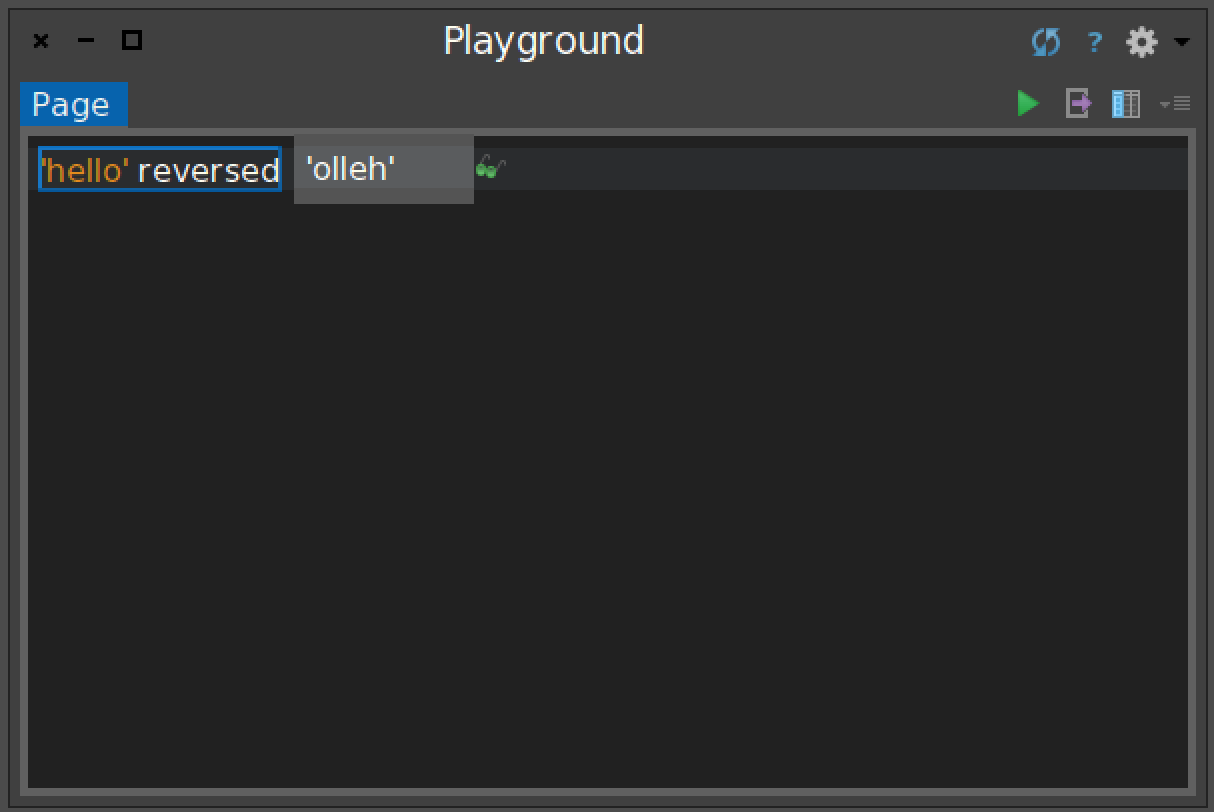
\includegraphics[width=0.7\textwidth]{/Users/ducasse/Workspace/FirstCircle/MyBooks/Bk-Writing/PharoBooks/LearningOOPWithPharoTrans/_result/pdf/Chapters/GettingStarted/figures/Editing.png}\caption{Executing an expression in Playground.\label{fig:Editing}}\end{center}
\end{figure}

\subsection{Other messages \& return values}
Our \textcode{'hello'} string understands many other messages than \textcode{reversed}:

\begin{displaycode}{plain}
'hello' asUppercase
>>> 'HELLO'
\end{displaycode}

As the name implies, the \textcode{asUppercase} message returns yet another string \textcode{'HELLO'}, which has the same contents as the receiver with each character converted to upper case.
However, messages sent to strings do not always return strings; other kinds of values are possible:

\begin{displaycode}{plain}
'hello' first
>>> $h

'hello' size
>>> 5
\end{displaycode}

The message \textcode{first} returns the first element of the string: a character.
Literal characters in Pharo syntax are expressed by the dollar sign \textcode{\$} immediately followed by the character itself.
The message \textcode{size} returns the number of elements in the string, which is an integer.

Strings, characters, integers are objects, because in Pharo \textit{everything} is an object.
Also, messages \textit{always} return something, even if the returned value is not used.
One might say that a message can return any value, as long as it's an object.
\subsection{The selector \& unary messages}
All messages we saw so far have the same receiver, the string \textcode{'hello'}; however, the computations were different because the messages differ by their name, or to use the technical term, by their \textit{selector}.
In the syntax of a message, the selector always comes right after the receiver; the message-sending syntax is just the white space in between!

Those messages are called \textit{unary} because they involve only one object: their receiver; they do not take any arguments.
Syntactically, the selectors of unary messages must be alphabetic words; the convention to make up longer selectors is to use lower camel case, preferring \textcode{asUppercase} over \textcode{as\_uppercase} or \textcode{AsUPPERCASE}.
\subsection{A first keyword-based message}
Messages often need to pass arguments to the receiver so that it can perform its task; this is what keyword-based messages are for.

As an example, instead of using \textcode{first}, we could use the message \textcode{at:}, with an explicit position as a parameter:

\begin{displaycode}{plain}
'hello' at: 1
>>>$h
\end{displaycode}

The selector \textcode{at:} consists of a single keyword that ends with a colon, signifying that it should be followed by an argument; in this case, an integer indicating which element we want to access.
Pharo counts indices starting from 1; therefore the message \textcode{at: 2} will access the second element of the receiver.

\begin{displaycode}{plain}
'hello' at: 2
>>>$e
\end{displaycode}
\subsection{Keyword-based messages with multiple arguments}
To pass more than one argument, a single message can have as many colon-terminated keywords as necessary, each followed by an argument, like this:

\begin{displaycode}{plain}
'hello' copyFrom: 1 to: 3
>>> 'hel'
\end{displaycode}

This is one single message, whose selector is really \textcode{copyFrom:to:}.
Note how naturally it reads and how, with well-chosen terms, each keyword of the selector documents the argument that follows it.

In the syntax, you are free to use as much white space as needed between the keywords and the arguments, and like unary messages, the convention is to name each keyword using lower camel case.
\subsection{Binary messages}
Binary messages visually differ from the other two kinds because their selectors can only be composed of symbols.
They always expect a single argument, even though they do not end in a colon.

The main use of binary messages is as arithmetic operations, for instance sending the message \textcode{+} to the integer \textcode{1}, with \textcode{2} as argument:

\begin{displaycode}{plain}
1 + 2
\end{displaycode}

But there are some other widely-used binary messages outside of arithmetics; for example, the message (selector) for string concatenation is a single comma:

\begin{displaycode}{plain}
'Hello' , ' Pharoers'
>>> 'Hello Pharoers'
\end{displaycode}

Here, the receiver is \textcode{'Hello'} and \textcode{' Pharoers'} is the argument.

\begin{coffee}
The \textit{receiver} is the object to which a message is sent; it is always first in a message, followed by the \textit{selector} and arguments.
\end{coffee}

\begin{coffee}
\textit{Unary messages} look like words and have no parameters beside their receiver. \textit{Binary messages} have selectors made of symbols and have one parameter. \textit{Keyword messages} take a parameter after each colon in their selector.
\end{coffee}

\begin{coffee}
A message is composed of a receiver, a message name, called its selector and optional arguments. By language abuse, we sometimes use message when in fact we mean the selector of the message. \textcode{,} is a message selector and \textcode{'a' ,'b'} is a message. 
\end{coffee}

\begin{coffee}
The preferred naming convention for unary and keyword selectors is lower camel case, \textcode{likeThis:orThat:}.
\end{coffee}
\section{Which message is executed first?}
Simpler messages take precedence over the more complex ones.
This very simple rule determines execution order when messages of different kinds appear in the same expression.
This means that unary messages are evaluated first, then binary messages, and finally keyword-based messages.

Together, the message syntax and precedence rules keep complex expressions elegant and readable:

\begin{displaycode}{plain}
'string' asUppercase copyFrom: -1 + 2 to: 6 - 3
>>> STR
\end{displaycode}

When message precedence does not match what you mean, you can force the execution order using parentheses.
In the following example, the expression inside the parentheses is evaluated first; this yields a three-character string \textcode{'STR'}, which then receives the message \textcode{reversed}.

\begin{displaycode}{plain}
('string' asUppercase first: 9 / 3) reversed
>>> 'RTS'
\end{displaycode}

Finally, note how \textcode{copyFrom:to:} and \textcode{first:} were sent to the result of \textcode{asUppercase}.
All messages are expressions whose result can be the receiver of a subsequent message; this is called \textit{message chaining}.
Unless the precedence rule applies, chained messages execute in reading order, from left to right.
This is quite natural for unary messages:

\begin{displaycode}{plain}
'abcd' allButFirst reversed
>>> 'dcb'

'abcd' reversed allButFirst
>>> 'cba'
\end{displaycode}

Note however that the chaining rule applies without exception, even to binary messages that look like arithmetic operators:

\begin{displaycode}{plain}
1 + 2 * 10
>>> 30
\end{displaycode}

Finally, keyword messages cannot be chained together without using parentheses, since the chain would look like a single big keyword message.
\section{Sending messages to classes}
Where do new objects come from?
Well, in Pharo, object creation is just another form of computation, so it happens by sending a message to the class itself.
For example, we can ask the class \textcode{String} to create an empty string by sending it the message \textcode{new}.

\begin{displaycode}{plain}
String new
>>> ''
\end{displaycode}

Classes are really objects that are known by name, so they provide a useful entry point to the system; creating new objects is just a particular use-case.
Some classes understand messages that return specific instances, like the class \textcode{Float} that understands the message \textcode{pi}.

\begin{displaycode}{plain}
Float pi
>>> 3.141592653589793
\end{displaycode}

\begin{coffee}
The naming convention for class names is upper camel case, \textcode{LikeThis}; this is the convention for all non-local names, i.e. shared or global variables.
\end{coffee}
\section{Local variables and statement sequences}
Local variables are declared by writing their name between vertical bars; their value can be set using the assignment statement \textcode{:=}.
Successive statements are \textit{separated} using a period, which makes them look like sentences.

\begin{displaycode}{plain}
| anArray |
anArray := Array new: 3.
anArray at: 1 put: true.
anArray at: 2 put: false.
anArray
>>> #(true false nil)
\end{displaycode}

In the code above, a new three-element array is created, and a reference to it is stored in \textcode{anArray}.
Then, its first two elements are set using the \textcode{at:put:} message, leaving the last element uninitialized; indexing is one-based, like normal humans count.

The final statement determines the value of the whole sequence; it is shown using the syntax for literal arrays \textcode{\#( … )}.
The first element is the boolean constant \textcode{true}, the second its counterpart \textcode{false}.
Uninitialised elements remain \textcode{nil}, the undefined object constant.

\begin{coffee}
The first element of a collection is at index \textcode{1}.
\end{coffee}

\begin{coffee}
The naming convention for local variables is lower camel case; variable names often start with an indefinite article, since they refer to otherwise anonymous objects.
\end{coffee}

\begin{coffee}
There are \textit{only six reserved keywords}, and all are pseudo-variables: the \textcode{true}, \textcode{false}, and \textcode{nil} object constants, and \textcode{self}, \textcode{super} and \textcode{thisContext}, which we talk about later.
\end{coffee}
\section{About literal objects}
Most objects in Pharo are created programmatically, by sending a message like \textcode{new} to a class.
In addition, the language syntax supports creating certain objects by directly expressing them in the code.
For example the expression  \textcode{\#(true false nil)} is equivalent to the previous snippet using \textcode{Array new}.

In the same way, \textcode{\$A} is equivalent to \textcode{Character codePoint: 65}:

\begin{displaycode}{plain}
Character codePoint: 65
>>> $A
\end{displaycode}
\section{Sending multiple messages to the same object}
We often need to send multiple messages to the same receiver, in close succession.
For instance, to build a long string without doing too many concatenations, we use a stream:

\begin{displaycode}{plain}
| aStream |
aStream := (String new: 100) writeStream.
aStream nextPutAll: 'Today, '.
aStream nextPutAll: Date today printString.
aStream contents
>>> 'Today, 28 January 2017'
\end{displaycode}

Repeating \textcode{aStream} is tedious to read.
To make this flow better, we group the three messages into a \textit{message cascade}, separating them with semicolons, and stating the receiver only once at the beginning:

\begin{displaycode}{plain}
| aStream |
aStream := (String new: 100) writeStream.
aStream 
	nextPutAll: 'Today, ';
	nextPutAll: Date today printString;
	contents
>>> 'Today, 28 January 2017'
\end{displaycode}

Like with statement sequences, the cascade as a whole returns the value of its last message.
Here is another example and its cascaded version:

\begin{displaycode}{plain}
| anArray |
anArray := Array new: 2. 
anArray at: 1 put: true.
anArray at: 2 put: false.
anArray
>>> #(true false)
\end{displaycode}

\begin{displaycode}{plain}
(Array new: 2)
	at: 1 put: true;
	at: 2 put: false;
	yourself
>>> #(true false)
\end{displaycode}

	
The three indented messages form a cascade; they are all sent to the same object, the new array.
The last message, \textcode{yourself}, is particularly useful to conclude cascades, because it returns the object it is sent to.
This is necessary in this case because the \textcode{at:put:} message would return the assigned element, not the array.
\section{Blocks}
Square brackets \textcode{{[}} and \textcode{{]}}  specify \textit{blocks} (also known as lexical closures), pieces of code to be executed later on.

In the following example, the adder local variable is assigned a one argument block. The code inside the block describes the variables it accepts \textcode{:x} and the statements to be executed when it is evaluated \textcode{x + 1}. Evaluating a block is done by sending a message, \textcode{value:} with an actual object as argument. The argument gets bound to the variable and the block is executed, resulting in 101.

\begin{displaycode}{plain}
| adder |
adder := [ :x | x + 1 ].
adder value: 100
>>> 101
adder value: 200
>>> 201
\end{displaycode}

\begin{important}
Technically, blocks are \textit{lexical closures}. Now in a first understanding, they represent kind of anonymous methods that can be stored, passed as arguments, and executed on demand using the messages \textcode{value}, \textcode{value:}...
\end{important}
\section{Control structures}
Blocks are used to express all control structures, from standard conditionals and loops to the exotic application specific ones, using the normal messaging syntax. For example loops and conditions are all expressed using the message presented previously. There are many loops and conditional in Pharo but they are all using the same principle: a block is passed as argument and the loop definition defines when the block should be executed. 

The message \textcode{timesRepeat}: executes multiple time its argument (a block).
Here we multiply by two a number 10 times. 

\begin{displaycode}{plain}
n := 1.
10 timesRepeat: [ n := n * 2 ].
n 
>>> 1024
\end{displaycode}

Conditionals are expressed by sending one of the messages \textcode{ifTrue:},
\textcode{ifFalse:}, \textcode{ifTrue:ifFalse:}, or \textcode{ifFalse:ifTrue:} to the result of a boolean expression.

\begin{displaycode}{plain}
(17 * 13 > 220)
	ifTrue: [ 'bigger' ]
	ifFalse: [ 'smaller' ] 
>>>'bigger'
\end{displaycode}

The message \textcode{do:} allows one to express a loop over a sequence of objects: a block is executed on each of the elements. 

Let us see how we can count the number of character \textcode{i} in a given string. On each character we check 
if the character is an \textcode{\$i} and increase the counter value if this is the case. 

\begin{displaycode}{plain}
| count |
count := 0.
'Fear is the little-death that brings total obliteration'
	 do: [:c | c == $i ifTrue: [count := count + 1]].
count
>>> 5
\end{displaycode}
\section{Methods}

\begin{figure}

\begin{center}
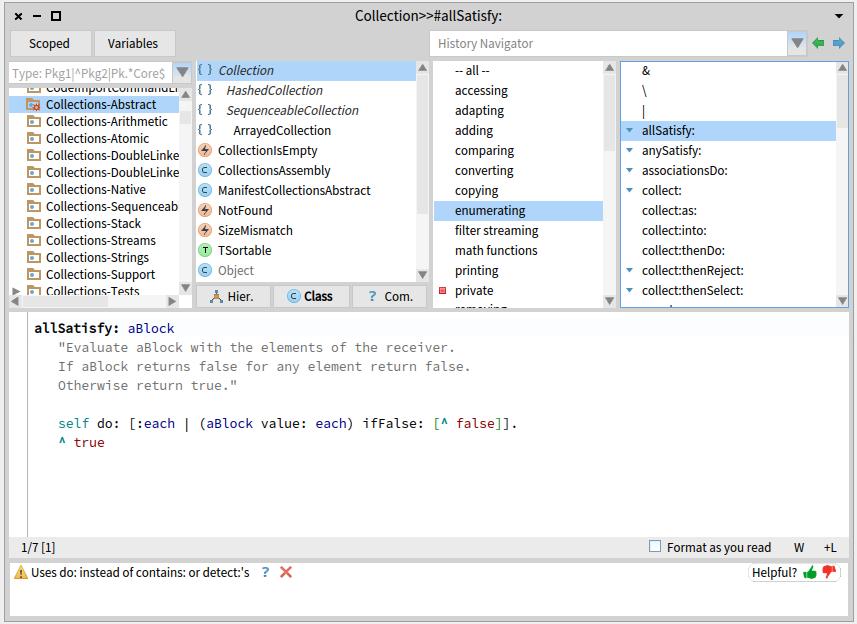
\includegraphics[width=0.95\textwidth]{/Users/ducasse/Workspace/FirstCircle/MyBooks/Bk-Writing/PharoBooks/LearningOOPWithPharoTrans/_result/pdf/Chapters/GettingStarted/figures/allSatisfy.png}\caption{Reading or editing a method using a code browser. Topleft pane: list of packages then list of classes then protocols then method lists - middle pane: method definition. Last pane: Quality Assistant.\label{fig:allSatisfy}}\end{center}
\end{figure}


Imagine that we want to check that all the objects in a collection hold a given property.
Here we check that all the numbers in the array are even numbers.

\begin{displaycode}{plain}
#(2 4 8 16 32) allSatisfy: [ :each | each even ]
>>> true
\end{displaycode}

But the following is false because not all the numbers are odd.  

\begin{displaycode}{plain}
#(1 2 3 4 5 6) allSatisfy: [ :each | each odd ]
>>> false
\end{displaycode}

The message \textcode{allSatisfy:} is one of the many super powerful behaviors implemented in \textcode{Collection}. It is called an iterator.

Methods are edited one by one in a code browser, like the one shown in Figure \ref{fig:allSatisfy}.

The following code is the definition of the method \textcode{allSatisfy:} in the class \textcode{Collection}. The first line specifies the method name, the selector, with names for all arguments. Comments are surrounded by double quotes. Inside a method, \textcode{self} refers to the object itself, the receiver.

\begin{displaycode}{plain}
allSatisfy: aBlock
	"Evaluate aBlock with the elements of the receiver.
	If aBlock returns false for any element return false.
	Otherwise return true."
	self do: [:each | (aBlock value: each) ifFalse: [^ false]].
	^ true
\end{displaycode}

Let us explain the implementation of this method. Using the message \textcode{do:} we iterate over all elements of the collection. For each element we execute block (a predicate) that returns a boolean value and act accordingly. As soon as we get a false value, we stop and return an overall false value. If every evaluation gave us true, we passed the whole test and can return \textcode{true} as the overall result.

In a method, the receiver (\textcode{self}) is the default return value of the whole method. Using a caret (\textcode{\string^}) in a method allows to return something else, or to return earlier.
\section{Resources}
This chapter showed you the key syntactic elements. If you want to get a deeper understanding about the syntax please refer to the following mooc videos. The Mooc on Pharo is available at \url{http://mooc.pharo.org}

Here are direct pointers to the videos we believe will help you to understand the Pharo syntax and key messages: 

\begin{itemize}
\item Syntax in a nutshell \url{http://rmod-pharo-mooc.lille.inria.fr/MOOC/Videos/W1/C019SD-W1-S5-v2.mp4}
\item Understanding messages \url{http://rmod-pharo-mooc.lille.inria.fr/MOOC/Videos/W2/C019SD-W2-S1-v3.mp4}
\item Pharo for the Java Programmer \url{http://rmod-pharo-mooc.lille.inria.fr/MOOC/Videos/W2/C019SD-W2-S2-v3.mp4}
\item Message precedence \url{http://rmod-pharo-mooc.lille.inria.fr/MOOC/Videos/W2/C019SD-W2-S3-v3.mp4}
\item Sequence and cascade \url{http://rmod-pharo-mooc.lille.inria.fr/MOOC/Videos/W2/C019SD-W2-S3-v3.mp4}
\item Blocks \url{http://rmod-pharo-mooc.lille.inria.fr/MOOC/Videos/W2/C019SD-W2-S6-v2.mp4}
\item Loops \url{http://rmod-pharo-mooc.lille.inria.fr/MOOC/Videos/W2/C019SD-W2-S7-v2.mp4}
\item Booleans and collections \url{http://rmod-pharo-mooc.lille.inria.fr/MOOC/Videos/W2/C019SD-W2-S8-v2.mp4}
\item Class and Method Definition \url{http://rmod-pharo-mooc.lille.inria.fr/MOOC/Videos/W1/C019SD-W1-S6-v3.mp4}
\item Understanding return \url{http://rmod-pharo-mooc.lille.inria.fr/MOOC/Videos/W3/C019SD-W3-S11-v1.mp4}
\item Parentheses \url{http://rmod-pharo-mooc.lille.inria.fr/MOOC/Videos/W2/C019SD-W2-S9-v3.mp4}
\item Yourself \url{http://rmod-pharo-mooc.lille.inria.fr/MOOC/Videos/W2/C019SD-W2-S10-v3.mp4}
\item Variables \url{http://rmod-pharo-mooc.lille.inria.fr/MOOC/Videos/W3/C019SD-W3-S3-v3.mp4}
\item Essential collections \url{http://rmod-pharo-mooc.lille.inria.fr/MOOC/Videos/W3/C019SD-W3-S7-v3.mp4} 
\item Iterators \url{http://rmod-pharo-mooc.lille.inria.fr/MOOC/Videos/W3/C019SD-W3-S9-v3.mp4}
\end{itemize}
\section{Conclusion }
You have three kinds of messages and the simpler are executed prior to more complex one. Hence unary messages are executed before binary and binary before keyword-based messages. 
Blocks are anonymous methods that can be pass around and used to define control structures and loops.

You now know enough to read 95\% of Pharo code. Remember, it is all just messages being sent to objects.
\chapter{Syntax summary}\subsection{Six reserved words only}
\begin{tabular}{ll}
\toprule
\textcode{nil} & the undefined object \\
\textcode{true}, \textcode{false} & boolean objects \\
\textcode{self} & the receiver of the current message \\
\textcode{super} & the receiver, in the superclass context \\
\textcode{thisContext} & the current invocation on the call stack \\
\bottomrule
\end{tabular}
\subsection{Reserved syntactic constructs}
\begin{tabular}{ll}
\toprule
\textcode{\symbol{34}comment\symbol{34}} & comment \\
\textcode{'string'} & string \\
\textcode{\#symbol} & unique string \\
\textcode{\$a}, Character space & the character a and a space \\
12 2r1100 16rC & twelve (decimal, binary, hexadecimal) \\
3.14 1.2e3 & floating-point numbers \\
\textcode{\#(abc 123)} & literal array with the symbol \textcode{\#abc} and the number 123 \\
\textcode{\{foo . 3 + 2\}} & dynamic array built from 2 expressions \\
\textcode{\#{[}123 21 255{]}} & byte array \\
\textit{exp1}. \textit{exp2} & expression separator (period) \\
\textcode{;} & message cascade (semicolon) \\
var := \textit{expr} & assignment \\
\textcode{\string^} \textit{expr} & return a result from a method (caret) \\
\textcode{{[} :e \textbar{} expr {]}} & code block with a parameter \\
\textcode{\textbar{} var1 var2 \textbar{}} & declaration of two temporary variables \\
\bottomrule
\end{tabular}
\subsection{Message Sending}
When we send a message to an object, the message
\textit{receiver}, the method is selected and executed; the message returns an object. Messages syntax mimics natural languages, with a subject, a verb, and complements. 

		

\begin{tabular}{ll}
\toprule
\textbf{Java} & \textbf{Pharo} \\
\textcode{aColor.setRGB(0.2,0.3,0)} & \textcode{aColor r: 0.2 g: 0.3 b: 0 } \\
\textcode{d.put(\symbol{34}1\symbol{34}, \symbol{34}Chocolate\symbol{34}); } & \textcode{d at: '1' put: 'Chocolate'} \\
\bottomrule
\end{tabular}
\subsection{Three Types of Messages: Unary, Binary, and Keyword}
A \textbf{unary} message is one with no arguments.

\begin{displaycode}{plain}
Array new
>>> anArray
\end{displaycode}

\begin{displaycode}{plain}
#(4 2 1) size
>>> 3
\end{displaycode}

\textcode{new} is an unary message sent to classes (classes are objects). 

A \textbf{binary} message takes only one argument and is named by one or more symbol characters from \textcode{+}, \textcode{-}, \textcode{*}, \textcode{= }, \textcode{\textless{}}, \textcode{\textgreater{}}, ...

\begin{displaycode}{plain}
3 + 4
>>> 7 
\end{displaycode}

\begin{displaycode}{plain}
'Hello' , ' World'
>>>'Hello World'
\end{displaycode}

The \textcode{+} message is sent to the object 3 with 4 as
 argument. The string 'Hello'receives the message \textcode{,}
(comma) with \textcode{' World'} as the argument.

A \textbf{keyword} message can take one or more
arguments that are inserted in the message name.

\begin{displaycode}{plain}
'Pharo' allButFirst: 2
>>> 'aro'
\end{displaycode}

\begin{displaycode}{plain}
3 to: 10 by: 2
>>> (3 to: 10 by: 2)
\end{displaycode}

The second example sends
\textcode{to:by:} to 3, with arguments 10 and 2; this
returns an interval containing 3, 5, 7, and 9.
\subsection{Message Precedence}
Parentheses \textcode{\textgreater{}} unary \textcode{\textgreater{}} binary \textcode{\textgreater{}} keyword, and finally from
left to right.

\begin{displaycode}{plain}
(15 between: 1 and: 2 + 4 * 3) not
>>> false
\end{displaycode}

Messages \textcode{+} and \textcode{*} are sent first, then \textcode{between:and:} is sent, and \textcode{not}.
The rule suffers no exception: operators are just binary messages with \textit{no notion of mathematical precedence}. 2 + 4 * 3 reads left-to-right and gives 18, not 14!
\subsection{Cascade: Sending Muliple Messages to the Same Object}
Multiple messages can be sent to the same receiver with ;.

\begin{displaycode}{plain}
OrderedCollection new
  add: #abc;
  add: #def;
  add: #ghi.
\end{displaycode}

The message \textcode{new} is sent to \textcode{OrderedCollection} which 
returns a new collection to which three
add: messages are sent. The value of the whole message cascade
is the value of the last message sent (here, the symbol
\textcode{\#ghi}). To return the receiver of the
message cascade instead (i.e. the collection), make sure to send
\textcode{yourself} as the last message of the cascade.
\subsection{Blocks}
Blocks are objects containing code that is executed on demand. They are the basis for control structures like conditionals and loops.

\begin{displaycode}{plain}
2 = 2
  ifTrue: [ Error signal: 'Help' ]
\end{displaycode}

\begin{displaycode}{plain}
#('Hello World')
  do: [ :e | Transcript show: e ]
\end{displaycode}

The first example sends the message \textcode{ifTrue:} to the boolean \textcode{true} (computed from
2 = 2) with a block as argument. Because the boolean is true,
the block is executed and an exception is signaled. The next example
sends the message \textcode{do:} to an array. This evaluates the block
once for each element, passing it via the e parameter. As a
result, \textcode{Hello World} is printed.
\subsection{Common Constructs: Conditionals}
In Java

\begin{displaycode}{plain}
if (condition)
	{ action(); }
	else { anotherAction();} 
\end{displaycode}

In Pharo

\begin{displaycode}{plain}
condition
	ifTrue: [ action ]
	ifFalse: [ anotherAction ]
\end{displaycode}

In Java

\begin{displaycode}{plain}
while (condition) { action(); 
     anotherAction(); }
\end{displaycode}

In Pharo

\begin{displaycode}{plain}
[ condition ] whileTrue: [ action. anotherAction ]
\end{displaycode}
\subsection{Common Constructs: Loops/Iterators}
In Java

\begin{displaycode}{plain}
for(int i=1; i<11; i++){
    System.out.println(i); } 
\end{displaycode}

In Pharo

\begin{displaycode}{plain}
1 to: 11 do: [ :i | Transcript show: i ; cr ] 
\end{displaycode}

In Java

\begin{displaycode}{plain}
String [] names ={"A", "B", "C"};
for( String name : names ) { 
     System.out.print( name );  
     System.out.print(","); }  
\end{displaycode}

In Pharo

\begin{displaycode}{plain}
| names | 
names := #('A' 'B' 'C').
names do: [ :each | Transcript show: each, ' , ' ]
\end{displaycode}

Collections start at 1. Messages \textcode{at: index} gives element at index and \textcode{at: index put: value} sets element at index to value.

\begin{displaycode}{plain}
#(4 2 1) at: 3
>>> 1 
\end{displaycode}

\begin{displaycode}{plain}
#(4 2 1) at: 3 put: 6
>>>#(4 2 6) 
\end{displaycode}

\begin{displaycode}{plain}
Set new add: 4; add: 4; yourself
>>> aSet 
\end{displaycode}
\subsection{Files and Streams}
\begin{displaycode}{plain}
work := FileSystem disk workingDirectory. 
stream := (work / 'foo.txt') writeStream. 
stream nextPutAll: 'Hello World'. 
stream close. 
stream := (work / 'foo.txt') readStream. 
stream contents. 
>>> 'Hello World' 
stream close.
\end{displaycode}
\chapter{Challenge yourself}\label{cha:challenging}
In Pharo everything is an object and most computation happens by sending  \textit{messages} to objects. In this chapter we propose a list of exercises to challenge you with the syntax.
\section{Challenge: Message identification}
For each of the expressions below, fill in the answers:

\begin{itemize}
\item What is the receiver object?
\item What is the message selector?
\item What is/are the argument (s)?
\item What is the result returned by this expression execution?
\end{itemize}

\begin{displaycode}{plain}
3 + 4

	receiver: 
	selector:
	arguments:
	result:
\end{displaycode}

\begin{displaycode}{plain}
Date today

	receiver: 
	selector:
	arguments:
	result:
\end{displaycode}

\begin{displaycode}{plain}
#('' 'World') at: 1 put: 'Hello'

	receiver: 
	selector:
	arguments:
	result:
\end{displaycode}

\begin{displaycode}{plain}
#(1 22 333) at: 2

	receiver: 
	selector:
	arguments:
	result:
\end{displaycode}

\begin{displaycode}{plain}
#(2 33 -4 67) collect: [ :each | each abs ]

	receiver: 
	selector:
	arguments:
	result:
\end{displaycode}

\begin{displaycode}{plain}
25 @ 50

	receiver: 
	selector:
	arguments:
	result:
\end{displaycode}

\begin{displaycode}{plain}
SmallInteger maxVal


	receiver: 
	selector:
	arguments:
	result:
\end{displaycode}

\begin{displaycode}{plain}
#(a b c d e f) includesAll: #(f d b)

	receiver: 
	selector:
	arguments:
	result:
\end{displaycode}

\begin{displaycode}{plain}
true | false

	receiver: 
	selector:
	arguments:
	result:
\end{displaycode}

\begin{displaycode}{plain}
Point selectors

	receiver: 
	selector:
	arguments:
	result:
\end{displaycode}
\section{Challenge: Literal objects}
What kind of object does the following literal expressions refer to? It is the same as asking what is the result of sending the \textcode{class} message to such expressions. 

\begin{displaycode}{plain}
1.3

>
\end{displaycode}

\begin{displaycode}{plain}
#node1

>
\end{displaycode}

\begin{displaycode}{plain}
#(2 33 4)

>
\end{displaycode}

\begin{displaycode}{plain}
'Hello, Dave'

>
\end{displaycode}

\begin{displaycode}{plain}
[ :each | each scale: 1.5 ]

>
\end{displaycode}

\begin{displaycode}{plain}
$A 

>
\end{displaycode}

\begin{displaycode}{plain}
true

>
\end{displaycode}

\begin{displaycode}{plain}
1

>
\end{displaycode}
\section{Challenge: Kind of messages}
Examine the following messages and report if the message is unary, binary or keyword-based.

\begin{displaycode}{plain}
1 log

>
\end{displaycode}

\begin{displaycode}{plain}
Browser open

>
\end{displaycode}

\begin{displaycode}{plain}
2 raisedTo: 5

>
\end{displaycode}

\begin{displaycode}{plain}
'hello', 'world'

>
\end{displaycode}

\begin{displaycode}{plain}
10@20

>
\end{displaycode}

\begin{displaycode}{plain}
point1 x

> 
\end{displaycode}

\begin{displaycode}{plain}
point1 distanceFrom: point2

>
\end{displaycode}
\section{Challenge: Results}
Examine the following expressions. What is the value returned by the execution of the following expressions?

\begin{displaycode}{plain}
1 + 3 negated

>
\end{displaycode}

\begin{displaycode}{plain}
1 + (3 negated)

>
\end{displaycode}

\begin{displaycode}{plain}
2 raisedTo: 3 + 2

>
\end{displaycode}

\begin{displaycode}{plain}
| anArray |
anArray := #('first' 'second' 'third' 'fourth').
anArray at: 2


> 
\end{displaycode}

\begin{displaycode}{plain}
#(2 3 -10 3) collect: [ :each | each * each]

>
\end{displaycode}

\begin{displaycode}{plain}
6 + 4 / 2

>
\end{displaycode}

\begin{displaycode}{plain}
2 negated raisedTo: 3 + 2

>
\end{displaycode}

\begin{displaycode}{plain}
#(a b c d e f) includesAll: #(f d b)

>
\end{displaycode}
\section{Challenge: unneeded parentheses }
Putting more  parentheses than necessary is  a good way  to get started. Such  practice however leads to  less readable expressions. Rewrite the following expressions using the least number of parentheses. 

\begin{displaycode}{plain}
x between: (pt1 x) and: (pt2 y)


 ...
\end{displaycode}

\begin{displaycode}{plain}
((#(a b c d e f) asSet) intersection: (#(f d b) asSet))


 ...
\end{displaycode}

\begin{displaycode}{plain}
(x isZero)
     ifTrue: [....]
(x includes: y)
     ifTrue: [....]
	 




 ...
\end{displaycode}

\begin{displaycode}{plain}
(OrderedCollection new)
    add: 56; 
    add: 33; 
    yourself




 ...
\end{displaycode}

\begin{displaycode}{plain}
((3 + 4) + (2 * 2) + (2 * 3))


 ...
\end{displaycode}

\begin{displaycode}{plain}
(Integer primesUpTo: 64) sum


 ...
\end{displaycode}

\begin{displaycode}{plain}
('http://www.pharo.org' asUrl) retrieveContents


 ...
\end{displaycode}
\chapter{Developing a simple counter}
To get started in Pharo, we invite you to implement a simple counter by following the steps given below. In this exercise you will learn how to create packages classes, methods, instances. You will learn how to define tests and more. This simple tutorial covers most of the important actions that we do when developing in Pharo. 

Note that the development flow promoted by this little tutorial is \textit{traditional} in the sense that you will define a package, a class, \textit{then} define its instance variable \textit{then} define its methods \textit{and} finally execute it (See the companion video below). Now in Pharo, developers often follow a \textit{totally} different style (that we call live coding) where they execute an expression that raises errors and they code in the debugger and let the system define some instance variables and methods on the fly for them. Once you will have finished this tutorial, you will feel more confident with Pharo and we strongly suggest you to try the other style (See the second video showing such different development practices).
\subsection{Companion videos}
You can find at \url{http://mooc.pharo.org/}, the mooc videos with french and english voice over and subtitles in different languages (japanese, spanish, french, english).
Among such videos, two videos are related to the counter exercises. They are called \symbol{34}Redo\symbol{34} because this is left to the reader to follow and redo the 
videos. 

\begin{itemize}
\item Coding the traditional way: \url{http://rmod-pharo-mooc.lille.inria.fr/MOOC/Videos/W1/} and \url{http://rmod-pharo-mooc.lille.inria.fr/MOOC/Videos-EN/W2/}
\item Coding in the debugger: \url{http://rmod-pharo-mooc.lille.inria.fr/MOOC/Videos/W2/} and \url{http://rmod-pharo-mooc.lille.inria.fr/MOOC/Videos-EN/W2/}
\end{itemize}
\section{Our use case}
Here is our use case: we want to be able to create a counter, increment it twice, decrement it and check that its value is correct. It looks like this little use case will fit perfectly a unit test - you will define one later. 

\begin{displaycode}{plain}
| counter |
counter := Counter new.
counter increment; increment.
counter decrement.
counter count = 1
\end{displaycode}

Now we will develop all the mandatory class and methods to support this scenario.


\begin{figure}

\begin{center}
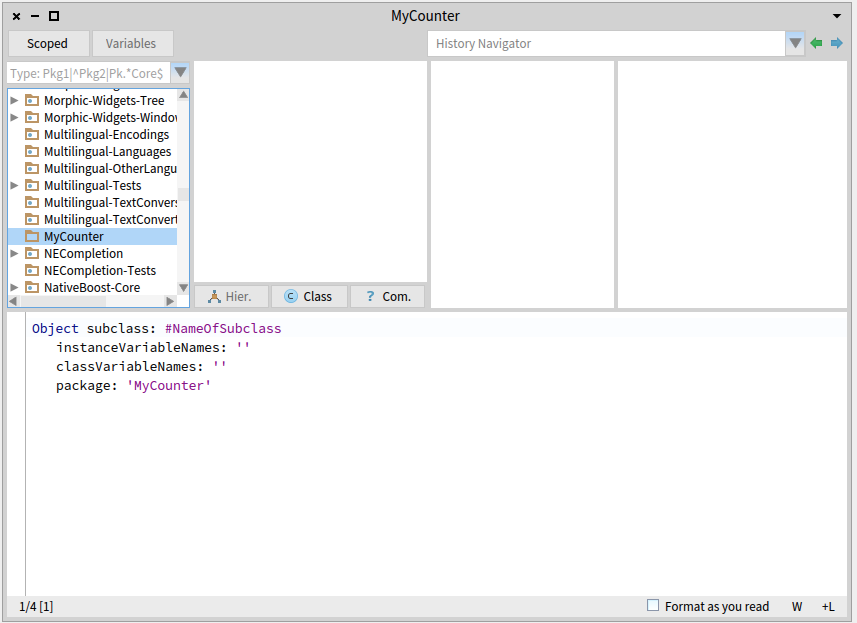
\includegraphics[width=1.0\textwidth]{/Users/ducasse/Workspace/FirstCircle/MyBooks/Bk-Writing/PharoBooks/LearningOOPWithPharoTrans/_result/pdf/Chapters/Counter/figures/CounterPackageCreated.png}\caption{Package created and class creation template.\label{figpackageCreated}}\end{center}
\end{figure}

\section{Create your own class}
In this part, you will create your first class. In Pharo, a class is defined in a package. You will create a package then a class. The steps we will do are the same ones every time you create a class, so memorize them well. 
\subsection{Create a package}
Using the Browser create a package. The system will ask you a name, write \textcode{MyCounter}. This new package is then created and added to the list. Figure \ref{figpackageCreated} shows the result of creating such a package.
\subsection{Create a class}
Creating a class requires four steps. They consist basically in editing the class definition template to specify the class you want to create.

\begin{itemize}
\item By default, the system helps you to define a subclass of the class \textcode{Object}. This is why it is written \textcode{Object subclass: \#NameOfSubclass}.
\end{itemize}

\begin{itemize}
\item \textbf{Class Name.} You should fill in the name of your class by replacing the word \textcode{NameOfSubclass} with the word \textcode{Counter}. Take care that the name of the class starts with a capital letter and that you do not remove the \#sign in front of \textcode{NameOfClass}. This is because the class we want to create does not exist yet, so we have to give its name, and we use a Symbol (a unique string in Pharo) to do so. 
\end{itemize}

\begin{itemize}
\item \textbf{Instance variable definition.} Then, you should fill in the names of the instance variables of this class. We need one instance variable called \textcode{count}. Take care that you leave the string quotes!
\end{itemize}

\begin{itemize}
\item \textbf{Class variable definition}. As we do not need any class variable make sure that the argument  for the class instance variables is an empty string \textcode{classInstanceVariableNames: ''}.
\end{itemize}

You should get the following class definition.

\begin{displaycode}{plain}
Object subclass: #Counter
   instanceVariableNames: 'count'
   classVariableNames: ''
   package: 'MyCounter'
\end{displaycode}

Now we should compile it. We now have a filled-in class definition for the class \textcode{Counter}. To define it, we still have to \textit{compile} it. Therefore, select the accept menu item. The class \textcode{Counter} is now compiled and immediately added to the system.

Figure \ref{figclassCreated} illustrates the resulting situation that the browser should show.

\begin{figure}

\begin{center}
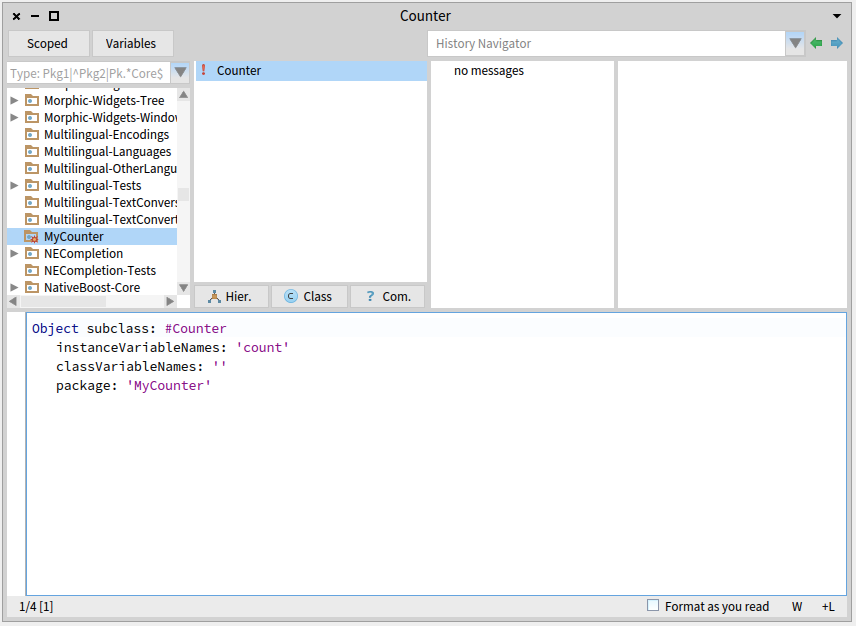
\includegraphics[width=1.0\textwidth]{/Users/ducasse/Workspace/FirstCircle/MyBooks/Bk-Writing/PharoBooks/LearningOOPWithPharoTrans/_result/pdf/Chapters/Counter/figures/CounterClassCreated.png}\caption{Class created.\label{figclassCreated}}\end{center}
\end{figure}


The tool runs automatically some code critic and some of them are just inaccurate, so do not care for now. 

As we are disciplined developers, we add a comment to \textcode{Counter} class by clicking Comment button. You can write the following comment:

\begin{displaycode}{plain}
Counter is a simple concrete class which supports incrementing and decrementing a counter.
Its API is 
- decrement, increment
- count
Its creation API is message withValue: 
\end{displaycode}

Select menu item 'accept' to store this class comment in the class.
\section{Define protocols and methods}
In this part you will use the browser to learn how to add protocols and methods.

The class we have defined has one instance variable named \textcode{count}. You should remember that in Pharo, (1) everything is an object, (2)  instance variables are private to the object, and (3) the only way to interact with an object is by sending messages to it.

Therefore, there is no other mechanism to access the instance variable values from outside an object than sending a message to the object. What you can do is to define messages that return the value of the instance variable. Such methods are called \textit{accessors}, and it is a common practice to always define and use them. We start to create an accessor method for our instance variable \textcode{count}.

A method is usually sorted into a protocol. These protocols are just a group of methods without any language semantics, but convey important navigation information for the reader of your class. You get protocol named: \textcode{'testing'} for method performing tests, \textcode{'printing'} for methods displaying the object, \textcode{'accessing'} for simple accessor methods and so on. 

Although protocols can have any name, Pharo programmers follow certain conventions for naming these protocols. But don't be stressed if you do not name well your protocols. 
\subsection{Create a method}
Now let us create the accessor methods for the instance variable \textcode{count}. Start by selecting the class \textcode{Counter} in a browser, and make sure that you are editing the instance side of the class (i.e., we define methods that will be sent to instances) by deselecting the Class side radio button.

Create a new protocol by bringing the menu of methods protocol list: click on the third list from the left. Select the newly created protocol. Then in the bottom pane, the edit field displays a method template laying out the default structure of a method. As a general hint, double click at the end of or beginning of the text and start typing your method.
Replace the template with the following method definition:

\begin{displaycode}{plain}
count
   "return the current value of the value instance variable"
   ^ count
\end{displaycode}

This defines a method called \textcode{count}, taking no arguments, having a method comment and returning the instance variable \textcode{count}. Then choose \textit{accept} in the menu to compile the method. You can now test your new method by typing and evaluating the next expression in a Playground, or any text editor.

\begin{displaycode}{plain}
Counter new count
>>> nil
\end{displaycode}

This expression first creates a new instance of \textcode{Counter}, and then sends the message \textcode{count} to it. It retrieves the current value of the counter. This should return \textcode{nil} (the default value for non-initialised instance variables). Afterwards we will create instances with a reasonable default initialisation value.
\subsection{Adding a setter method}
Another method that is normally used besides the accessor method is a so-called setter method. Such a method is used to change the value of an instance variable from a client. For example, the expression \textcode{Counter new count: 7} first creates a new \textcode{Counter} instance and then sets its value to 7:

The snippets shows that the counter effectively contains its value.

\begin{displaycode}{plain}
| c |
c := Counter new count: 7.
c count
>>> 7
\end{displaycode}

This setter method does not currently exist, so as an exercise write the method \textcode{count:} such that, when invoked on an instance of \textcode{Counter},  instance variable is set to the argument given to the message. Test your method by typing and evaluating the expression above.
\section{Define a Test Class}
Writing tests is an important activity that will support the evolution of your application. Remember that a test is written \textit{once and executed million} times. For example if we have turned the expression above into a test we could have checked automatically that our new method is correctly working. 

To define a test case we will define a class that inherits from \textcode{TestCase}. Therefore define a class named \textcode{CounterTest} as follows:

\begin{displaycode}{plain}
TestCase subclass: #CounterTest
   instanceVariableNames: ''
   classVariableNames: ''
   package: 'MyCounter'
\end{displaycode}

Now we can write a first test by defining one method. Test methods should start with \textit{test} to be automatically executed by the TestRunner or when you press on the icon of the method. Now to make sure that you understand in which class we define the method we prefix the method body with the class name and \textcode{\textgreater{}\textgreater{}}.
\textcode{CounterTest\textgreater{}\textgreater{}} means that the method is defined in the class \textcode{CounterTest}.

Define the following method. It first creates an instance, sets its value and verifies that the value is correct. The message \textcode{assert:} is a special message verifying if the test passed or not.

\begin{displaycode}{plain}
CounterTest >> testCountIsSetAndRead
   | c |
   c := Counter new.
   c count: 7.
   self assert: c count = 7
\end{displaycode}

Verify that the test passes by executing either pressing the icon in front of the method or using the TestRunner available in the Tools menu (selecting your package).
Since you have a first green test. This is a good moment to save your work. 


\begin{figure}

\begin{center}
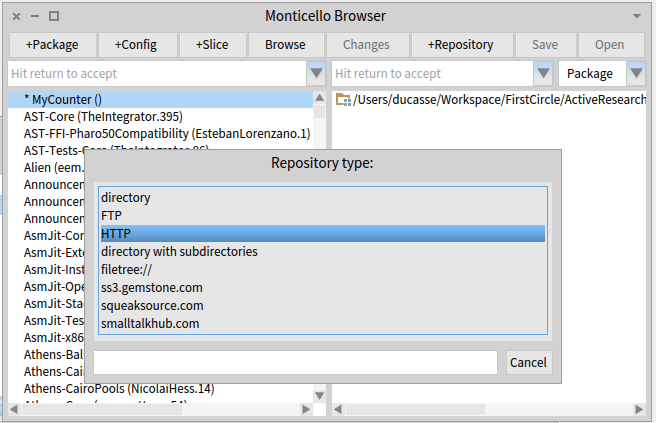
\includegraphics[width=1.0\textwidth]{/Users/ducasse/Workspace/FirstCircle/MyBooks/Bk-Writing/PharoBooks/LearningOOPWithPharoTrans/_result/pdf/Chapters/Counter/figures/CounterAddingRepo.png}\caption{Selecting a new kind of repository to the list of possible places to commit the package.\label{figSelectingARepo}}\end{center}
\end{figure}



\begin{figure}

\begin{center}
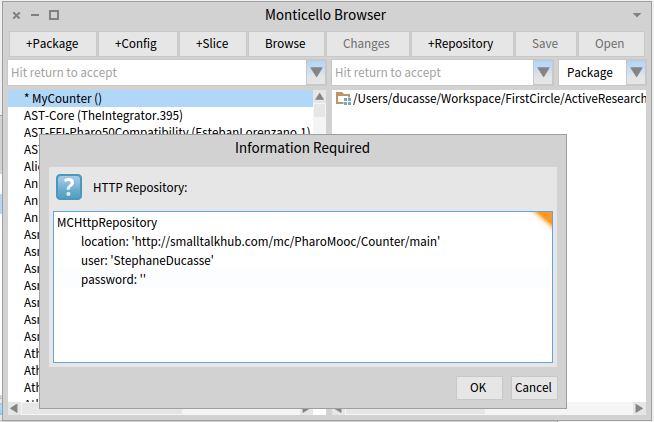
\includegraphics[width=1.0\textwidth]{/Users/ducasse/Workspace/FirstCircle/MyBooks/Bk-Writing/PharoBooks/LearningOOPWithPharoTrans/_result/pdf/Chapters/Counter/figures/CounterEditingProject.png}\caption{Editing the repository information.\label{figAddingARepo}}\end{center}
\end{figure}

\section{Saving your work}
Several ways to save your work exist. 

\begin{itemize}
\item \textit{Using plain files}. You can save the class or a method by clicking on it and selecting the fileout menu item. You will get a file containing the source code on your hard-disk - This is not the favorite way to save your code. 
\item \textit{Using a version control system}. It is better to use a version control system. In Pharo you can use Monticello and Git (even if it is more for advanced users).
\end{itemize}

In this chapter, we explain the simplest way to get you done. Note that the complete set of Pharo packages is managed via Monticello (which is a distributed versioning control system - there are chapters in \textbf{Pharo by Example} and \textbf{Deep into Pharo} books \url{http://books.pharo.org}).

Use the \textbf{Monticello Browser} (available in Tools) to save your work. You can save a package locally on your hard-disk or on a remote server on the web such as \url{http://www.smalltalkhub.com}
\subsection{Saving using Monticello}
Using Monticello you can save your work:

\begin{itemize}
\item \textit{Locally}. You can store your packages in a folder on your disk (use directory as a kind of repository below).
\item \textit{Remotely}. Using an account on a free server such \url{http://www.smalltalkhub.com/}. You can save your work and share it with others.
\end{itemize}

Note each time you load or save a package, this package is also be stored in the folder named 'package-cache' on your hard-disk.
\subsubsection{Add a repository}
Go to \url{http://www.smalltalkhub.com/} and create a member account then register a new project. You get an HTTP entry that refers to your project. Define a new HTTP repository using the Monticello Browser as shown by Figures \ref{figSelectingARepo} and \ref{figAddingARepo}.

Figure \ref{figSelectingARepo} shows that your package is dirty: this is indicated with the little '*' in front of the packages.

\textbf{Example.} As authors we  are saving the examples for this chapter as a special team named PharoMooc in the Counter project so our information is the following:  

\begin{displaycode}{plain}
MCHttpRepository
	location: 'http://smalltalkhub.com/mc/PharoMooc/Counter/main'
	user: ''
	password: ''
\end{displaycode}

Now for you, you should adapt the following template to use your own information: 

\begin{displaycode}{plain}
MCHttpRepository
	location: 'http://smalltalkhub.com/mc/YourAccount/YourProject/main'
	user: 'YourAccountID'
	password: 'YourAccountPassword'
\end{displaycode}
\subsubsection{Saving your package}
To save your work, simply select your package and the repository you want to save it to and save it using the Save button. This will open a dialog where you can give a comment, version numbers and blessing. From then on, other people can load it from there, in the same way that you would use cvs or other multi-user versioning systems. Saving the image is also a way to save your working environment, but not a way to version and publish it in a way that can be easily shared.

You can of course both publish your package (so that other people can load it, and that you can compare it with other versions, etc.) and save your image (so that next time that you start your image you are in the same working environment).
\section{Adding more messages}
Before implementing the following messages we define first a test.
We define one test for the method \textcode{increment} as follows:

\begin{displaycode}{plain}
CounterTest >> testIncrement
   | c |
   c := Counter new.
   c count: 0 ; increment; increment.
   self assert: c count = 2
\end{displaycode}

Here we create a counter, set its value to 0, send it the message increment two times and verify that we get a counter of value 2. 

Now you should implement some more methods. 

\begin{itemize}
\item Propose a definition for the method \textcode{increment} and implement it. 
\item Implement also a new test method for the method \textcode{decrement}.
\item Define the method \textcode{decrement} place it together with \textcode{increment} in the protocol \textcode{'operation'}.
\end{itemize}

Here are the possible definitions for such methods. 

\begin{displaycode}{plain}
Counter >> increment
   count := count + 1
\end{displaycode}

\begin{displaycode}{plain}
Counter >> decrement
   count := count - 1
\end{displaycode}


\begin{figure}

\begin{center}
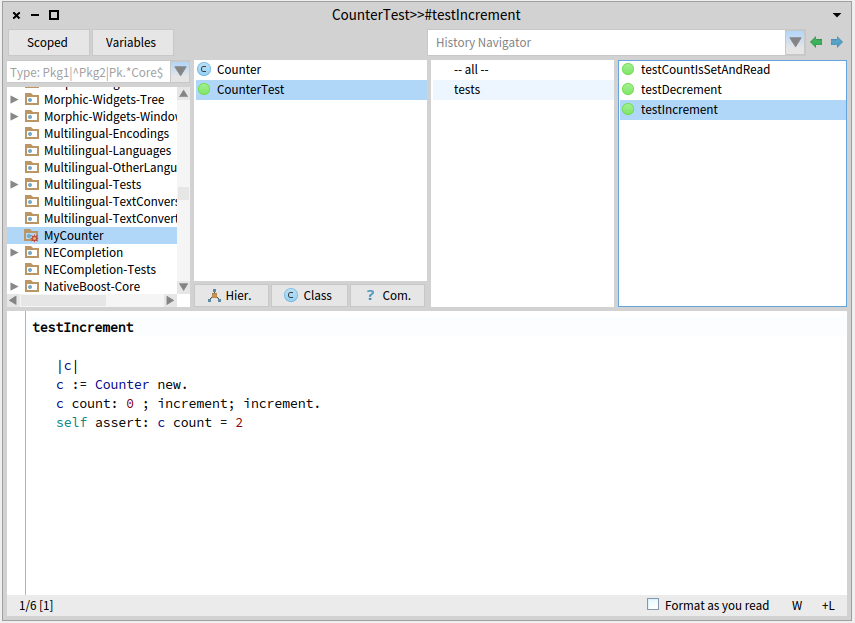
\includegraphics[width=1.0\textwidth]{/Users/ducasse/Workspace/FirstCircle/MyBooks/Bk-Writing/PharoBooks/LearningOOPWithPharoTrans/_result/pdf/Chapters/Counter/figures/CounterClassTestCreated.png}\caption{Class with green tests.\label{figclassTestCreated}}\end{center}
\end{figure}


Run your tests they should pass (as shown in Figure \ref{figclassTestCreated}). Again this is a good moment to save your work. Saving at point where tests are green
is always a good process. 
\section{Better object description}
When you select the expression \textcode{Counter new} and print its result (using the Print it menu of the editor) you obtain a simple string \textcode{'a Counter'}.

\begin{displaycode}{plain}
Counter new
>>> a Counter
\end{displaycode}

We would like to get a much richer information for example knowing the counter value. Implement the following methods in the protocol \textcode{printing}

\begin{displaycode}{plain}
Counter >> printOn: aStream
   super printOn: aStream.
   aStream nextPutAll: ' with value: ', self count printString.
\end{displaycode}

Note that the method \textcode{printOn:} is used when you print an object using print it (See Figure \ref{figBetterDescription}). In addition this method is invoked when you click on \textcode{self} in an inspector. An inspector is an object to interact and modify objects. It is really powerful during development.


\begin{figure}

\begin{center}
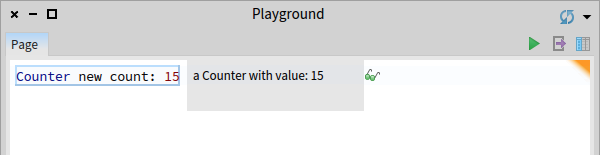
\includegraphics[width=1.0\textwidth]{/Users/ducasse/Workspace/FirstCircle/MyBooks/Bk-Writing/PharoBooks/LearningOOPWithPharoTrans/_result/pdf/Chapters/Counter/figures/CounterBetterDescription.png}\caption{Better description doing a Print It (cmd + P).\label{figBetterDescription}}\end{center}
\end{figure}

\section{Instance initialization method}
Right now the initial value of our counter is not set as the following expression shows it.

\begin{displaycode}{plain}
Counter new count
>>> nil
\end{displaycode}

Let us write a test checking that a newly created instance has 0 as a default value.

\begin{displaycode}{plain}
CounterTest >> testValueAtCreationTimeIsZero
   self assert: Counter new count = 0
\end{displaycode}

If you run it, it will turn yellow indicating a failure (a situation that you anticipated but that is not correct) - by opposition to an error which is an anticipated situation leading to failed assertion. 
\subsection{Define an initialize method}
Now we have to write an initialization method that sets a default value of the \textcode{count} instance variable. However, as we mentioned the \textcode{initialize} message is sent to the newly created instance. This means that the \textcode{initialize} method should be defined at the instance side as any method that is sent to an instance of \textcode{Counter} (like \textcode{increment}) and \textcode{decrement}. The \textcode{initialize} method is responsible to set up the default value of instance variables.

Therefore at the instance side, you should create a protocol \textcode{initialization}, and create the following method (the body of this method is left blank. Fill it in!).

\begin{displaycode}{plain}
Counter >> initialize
  "set the initial value of the value to 0"
  
  count := 0
\end{displaycode}

Now create a new instance of class \textcode{Counter}. Is it initialized by default? The following code should now work without problem:

\begin{displaycode}{plain}
Counter new increment
\end{displaycode}

and the following one should return 2

\begin{displaycode}{plain}
Counter new increment; increment; count
>>> 2
\end{displaycode}

Again save your work
\section{Conclusion}
In this chapter you learned how to define packages, classes, methods, and define tests.
The flow of programming that we chose for this first tutorial is similar to most of programming languages.
In Pharo you can use a different flow that is based on defining a test first, executing it and when the execution raises error to define the corresponding classes, methods, and instance variables often from inside the debugger. We suggest you now to redo the exercise following the second companion video.

\chapter{Tests, tests and tests}\label{cha:sunit}
In this chapter we start by showing that tests are simple. Second we present test driven design - basically what we will try to do systematically in this book. Then we discuss why we test, and what makes a good test.
We then present a series of small examples showing how to use SUnit. 
\section{Writing a test in 2 minutes}
A test is a context, a stimulus and an assertion (verification that we get the correct state).
Here is an example on sets. Remember that sets are mathematical entities having only one occurrence of their elements.

First we test that adding an element changes the size of the set.

\begin{itemize}
\item \textbf{Context:} we take an empty set.
\item \textbf{Stimulus:} we add \textcode{\$A} into the empty set.
\item \textbf{Assertion:} the set has one element.
\end{itemize}

Another test is that a set only contains only one occurence of one element.

\begin{itemize}
\item \textbf{Context:} we take an empty set.
\item \textbf{Stimulus:} we add \textcode{\$A} into the empty set.
\item \textbf{Assertion:} the set has one element.
\item \textbf{Stimulus:} we add \textcode{\$A} into the empty set.
\item \textbf{Assertion:} the set has still one element.
\end{itemize}
\subsection{How do we declare a test in Pharo?}
This is really easy to declare one test: we define one class (that will host multiple test definitions) and one method per test.

Here the class \textcode{MyExampleSetTest} should inherit from \textcode{TestCase}. It is the place to define the tests
related to the class \textcode{Set}. 

\begin{displaycode}{plain}
TestCase subclass: #MyExampleSetTest
	instanceVariableNames: ''
	classVariableNames: ''
	package: 'MySetTest'
\end{displaycode}

Now we can define one test expression as a method. There is one constraint: the method selector should start with \textcode{test}.

\begin{displaycode}{plain}
MyExampleSetTest >> testAddTwice
	| s |
	s := Set new. 
	self assert: s isEmpty.
	s add: $A.
	self assert: s size equals: 1.
	s add: $A.
	self assert: s size equals: 1.
\end{displaycode}

Then using the Test runner or pressing on icons of the Pharo browser (as shown in Figure \ref{fig:browsertests}), you will be able to execute the method \textcode{testAddTwice} and it will tell you if it passes or fails (i.e., if its assertions are true). Now that you know that writing a test is not complex. Let us look a bit at the theory before going into more details. 

\begin{coffee}
A test is a context, a stimulus and an \textit{assertion} (verification that we get the correct state).
\end{coffee}
\section{Test Driven Design}
The interest in testing and Test Driven Development is not limited to Pharo.
 Automated testing has become a hallmark of the \textit{Agile software
development} movement, and any software developer concerned with improving
software quality would do well to adopt it. Indeed, developers in many languages
have come to appreciate the power of unit testing.

Neither testing, nor the building of test suites, is new. By now, everybody knows that
tests are a good way to catch errors. By making testing a core practice and by emphasizing \textit{automated} tests, Extreme Programming has helped to make testing
productive and fun, rather than a chore that programmers dislike.

 The Pharo community has a long tradition of testing because of the incremental style of
development supported by its programming environment. In traditional Pharo
development, a programmer writes tests in a playground as soon as a method
was finished. Sometimes a test would be incorporated as a comment at the head of
the method that it exercised, or tests that needed some set up would be included
as example methods in the class. The problem with these practices is that tests
in a playground are not available to other programmers who modify the code.
Comments and example methods are better in this respect, but there is still no
easy way to keep track of them and to run them automatically. Tests that are not
run do not help you to find bugs! Moreover, an example method does not inform
the reader of the expected result: you can run the example and see the (perhaps
surprising) result, but you will not know if the observed behaviour is correct.

Using a testing framework such as SUnit  is valuable because it allows us to write tests that are self-checking:
the test itself defines what the correct result should be. It also helps us (1) to
organize tests into groups, (2) to describe the context in which the tests must run,
and (3) to run a group of tests automatically. As you saw, in less than two minutes you can
write tests using SUnit, so instead of writing small code snippets in a
playgound, we encourage you to use SUnit and get all the advantages of stored
and automatically executable tests.
\section{Why testing is important}\label{sec:whytest}
Now that you see that writing tests is simple. Let's step back and analyze the situation.
Unfortunately, many developers believe that tests are a waste of their time.
After all, \textit{they} do not write bugs, only \textit{other} programmers do that. Most
of us have said, at some time or other: \textit{I would write tests if I had more
time.} If you never write a bug, and if your code will never be changed in the
future, then indeed tests are a waste of your time. However, this most likely
also means that your application is trivial, or that it is not used by you or
anyone else. Think of tests as an investment for the future: having a test suite 
is quite useful now, but it will be \textit{extremely} useful when your
application, or the environment in which it runs, changes in the future.

Tests play several roles: 

\begin{itemize}
\item First, they provide documentation of the functionality that they cover. This documentation is active: watching the tests pass tells you that the documentation is up to date. 
\item Second, tests help developers to confirm that some changes that they have just made to a package have not broken anything else in the system, and to find the parts that break when that confidence turns out to be misplaced. 
\end{itemize}

\begin{itemize}
\item Finally, writing tests during, or even before, programming forces you to think about the functionality that you want to design, \textit{and how it should appear to the client code}, rather than about how to implement it.
\end{itemize}

By writing the tests first, i.e., before the code, you are compelled to state
the context in which your functionality will run, the way it will interact with the client code, and the expected results. Your code style will definitively improve.

Several software development methodologies such as \textit{eXtreme Programming} and
Test-Driven Development (TDD) advocate writing tests before writing code. This
may seem to go against your deep instincts as software developers. All we can say
is: go ahead and try it. Writing the tests before the code
helps you know what we want to code, helps you know when you are done, and helps
us conceptualize the functionality of a class and to design its interface.
Moreover, test-first development gives you the courage to change our application, because you will 
know when you break something.

We cannot test all aspects of any realistic application. Covering a complete
application is simply impossible and is the goal of testing. Even
with a good test suite some bugs will still creep into the application, where
they can lay dormant waiting for an opportunity to damage your system. If you
find that this has happened, take advantage of it! As soon as you uncover the
bug, write a test that exposes it, run the test, and watch it fail. Now you can
start to fix the bug: the test will tell you when you are done.
\section{What makes a good test?}
Writing good tests is a skill that you can learn by practicing.
Let us look at the properties that tests should have to get the maximum benefit.

\begin{itemize}
\item \textit{Tests should be repeatable.} You should be able to run a test as often as you want, and always get the same answer.
\end{itemize}

\begin{itemize}
\item \textit{Tests should run without human intervention}. You should be able to run them unattended.
\end{itemize}

\begin{itemize}
\item \textit{Tests should tell a story.} Each test should cover one aspect of a piece of code. A test should act as a scenario that you or someone else can read to understand a piece of functionality.
\end{itemize}

\begin{itemize}
\item \textit{Tests should have a change frequency lower than that of the functionality they cover}. You do not want to have to change all your tests every time you modify your application. One way to achieve this is to write tests based on the public interfaces of the class that you are testing. It is OK to write a test for a private \textit{helper} method if you feel that the method is complicated enough to need the test, but you should be aware that such a test may have to be changed, or thrown away entirely, when you think of a better implementation.
\end{itemize}

One consequence of such properties is that the number of tests should be
somewhat proportional to the number of functions to be tested: changing one
aspect of the system should not break all the tests but only a limited number.
This is important because having 100 tests fail should send a much stronger
message than having 10 tests fail. However, it is not always possible to achieve
this ideal: in particular, if a change breaks the initialization of an object,
or the set-up of a test, it is likely to cause all of the tests to fail.

Now let's go back and write a couple of tests using SUnit.
\section{SUnit by example}
We show a step by step example. We continue with the example that tests the class \textcode{Set}. Try editing and compiling the code as we go along. 

Pay attention: test classes are special classes. As subclasses of \textcode{TestCase} they have a different behavior that normal classes: their methods which start with \textcode{test} are automatically executed on newly created instances of the class. This is what happens when you press the icon close to the method in a class browser (as shown in Figure \ref{fig:browsertests}).
\subsection{Step 1: Create the test class}
We use the class \textcode{MyExampleSetTest} to group all the tests related to the class \textcode{Set}. First you should create a new subclass of \textcode{TestCase} called \textcode{MyExampleSetTest}. 

\begin{displaycode}{plain}
TestCase subclass: #MyExampleSetTest
	instanceVariableNames: ''
	classVariableNames: ''
	package: 'MySetTest'
\end{displaycode}
\subsection{Step 2: Write a test method}
Let's create some tests by defining some methods in the class
\textcode{MyExampleSetTest}. Each method represents one test. The names of the methods
should start with the string \textcode{'test'} so that SUnit collects them into
test suites. Test methods take no arguments.

Define the following test method named \textcode{testIncludes}. It tests
the \textcode{includes:} method of class \textcode{Set}. The test says that sending the message
\textcode{includes: 5} to a set containing 5 should return \textcode{true}. 

\begin{displaycode}{plain}
MyExampleSetTest >> testIncludes
	| full |
	full := Set with: 5 with: 6.
	self assert: (full includes: 5).
	self assert: (full includes: 6)
\end{displaycode}

As you see this is quite simple. Let's continue.
\subsection{Step 3: Run the test}
The easiest way to run the tests is directly from the browser. Simply click on
the icon of the class name, or on an individual test method, or use the  \textit{Run
tests (t)} . The test methods will be flagged green or red,
depending on whether they pass or not (as shown in Figure \ref{fig:browsertests}).


\begin{figure}

\begin{center}
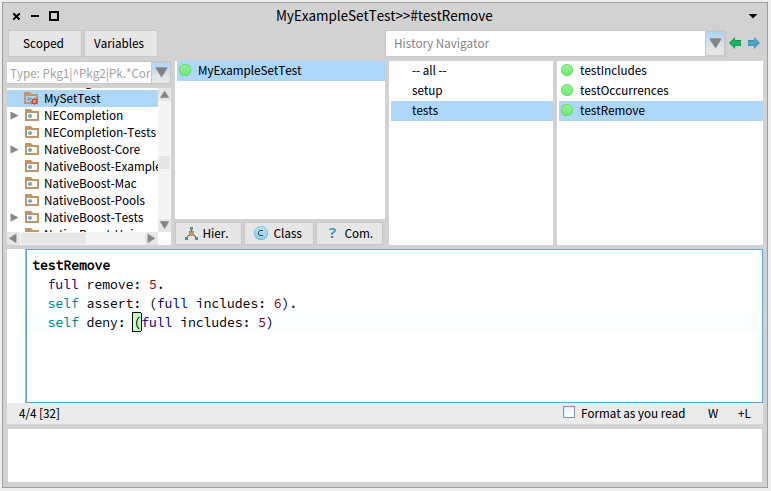
\includegraphics[width=0.8\textwidth]{/Users/ducasse/Workspace/FirstCircle/MyBooks/Bk-Writing/PharoBooks/LearningOOPWithPharoTrans/_result/pdf/Chapters/Tests/figures/updatedbrowsertests.png}\caption{Running SUnit tests from the System Browser: Just click on the round little button close to the class or method.\label{fig:browsertests}}\end{center}
\end{figure}

\subsection{Step 4: Write more tests}
Let's create more tests by defining some methods in the class
\textcode{MyExampleSetTest}.

The second test, named \textcode{testOccurrences}, verifies that the
number of occurrences of 5 in \textcode{full} set is equal to one, even if we
add another element 5 to the set.

\begin{displaycode}{plain}
MyExampleSetTest >> testOccurrences
	| empty full |
	empty := Set new.
	full := Set with: 5 with: 6.
	self assert: (empty occurrencesOf: 0) equals: 0.
	self assert: (full occurrencesOf: 5) equals: 1.
	full add: 5.
	self assert: (full occurrencesOf: 5) equals: 1
\end{displaycode}

Finally, we test that the set no longer contains the element 5 after we have
removed it.

\begin{displaycode}{plain}
MyExampleSetTest >> testRemove
	| full |
	full := Set with: 5 with: 6.
	full remove: 5.
	self assert: (full includes: 6).
	self deny: (full includes: 5)
\end{displaycode}

Note the use of the method \textcode{TestCase \textgreater{}\textgreater{} deny:} to assert something that should
not be true. \textcode{aTest deny: anExpression} is equivalent to
\textcode{aTest assert: anExpression not}, but is much more readable.
\subsection{Step 5: Run all the tests}
You can also select sets of test suites to run, and obtain a more detailed log
of the results using the SUnit Test Runner, which you can open by selecting the menu
\textcode{World \textgreater{} Test Runner}.

The \textit{Test Runner}, shown in Figure \ref{fig:test-runner}, is designed to make it easy to
execute groups of tests.

The left-most pane lists all of the packages that contain test classes (i.e.,
subclasses of \textcode{TestCase}). When some of these packages are selected, the test
classes that they contain appear in the pane to the right. Abstract classes are
italicized, and the test class hierarchy is shown by indentation, so subclasses
of \textcode{ClassTestCase} are indented more than subclasses of \textcode{TestCase}.
\textcode{ClassTestCase} is a class offering utilities methods to compute test
coverage.


\begin{figure}

\begin{center}
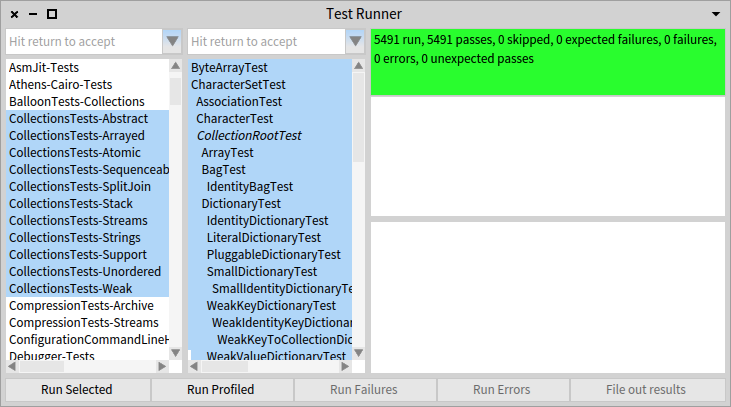
\includegraphics[width=0.8\textwidth]{/Users/ducasse/Workspace/FirstCircle/MyBooks/Bk-Writing/PharoBooks/LearningOOPWithPharoTrans/_result/pdf/Chapters/Tests/figures/updatedtestRunner.png}\caption{Running SUnit tests using the \textit{TestRunner}.\label{fig:test-runner}}\end{center}
\end{figure}


Open a Test Runner, select the package \textit{MySetTest}, and click the \textcode{Run Selected}
button.
\subsection{Step 6: Alternative ways to execute tests}
You can also run a single test (and print the usual pass/fail result summary) by executing a
\textit{Print it} on the following code: \textcode{MyExampleSetTest run: \#testRemove}.

Some people include an executable comment in their test methods as in \textcode{testRemove} below. For example the contents of the comment \textcode{self run: \#testRemove} can be executed: select the expression inside the comment (but not the comment) and bring the menu to do a \textit{Do it}.
It will execute the test. 

\begin{displaycode}{plain}
MyExampleSetTest >> testRemove
	"self run: #testRemove"
	| empty full |
	empty := Set new.
	full := Set with: 5 with: 6.
	full remove: 5.
	self assert: (full includes: 6).
	self deny: (full includes: 5)
\end{displaycode}
\subsection{Step 7: Looking at a bug}
Introduce a bug in \textcode{MyExampleSetTest \textgreater{}\textgreater{} testRemove} and run the tests again. For
example, change \textcode{6} to \textcode{7}, as in:

\begin{displaycode}{plain}
MyExampleSetTest >> testRemove
	| empty full |
	empty := Set new.
	full := Set with: 5 with: 6.
	full remove: 5.
	self assert: (full includes: 7).
	self deny: (full includes: 5)
\end{displaycode}

The tests that did not pass (if any) are listed in the right-hand panes of the
\textit{Test Runner}. If you want to debug one, to see why it failed, just click on
the name. Alternatively, you can execute one of the following expressions:

\begin{displaycode}{plain}
(MyExampleSetTest selector: #testRemove) debug

MyExampleSetTest debug: #testRemove
\end{displaycode}
\subsection{Step 8: Interpret the results}
The method \textcode{assert:} is defined in the class \textcode{TestAsserter}. This is a superclass
of \textcode{TestCase} and therefore all other \textcode{TestCase} subclasses and is responsible for
all kinds of test result assertions.
The \textcode{assert:} method expects a boolean argument, usually the value of a tested expression. When the
argument is true, the test passes; when the argument is false, the test fails.

There are actually three possible outcomes of a test: \textit{passing}, \textit{failing}, and \textit{raising an error}.

\begin{itemize}
\item \textbf{Passing}. The outcome that we hope for is that all of the assertions in the test are true, in which case the test passes. In the test runner, when all of the tests pass, the bar at the top turns green. 
\item \textbf{Failing}. The obvious way is that one of the assertions can be false, causing the test to \textit{fail}.
\item \textbf{Error}. The other possibility is that some kind of error occurs during the execution of the test, such as a \textit{message not understood} error or an \textit{index out of bounds} error. If an error occurs, the assertions in the test method may not have been executed at all, so we can't say that the test has failed; nevertheless, something is clearly wrong!
\end{itemize}

In the \textit{test runner}, failing tests cause the bar at the top to turn yellow, and are listed in the middle pane on
the right, whereas tests with errors cause the bar to turn red, and are listed in
the bottom pane on the right.

As an exercise, modify your tests to provoke both errors and failures.
\section{The SUnit cookbook}
This section will give you more details on how to use SUnit. If you have used
another testing framework such as JUnit, much of this will be familiar, since
all these frameworks have their roots in SUnit. Normally you will use SUnit's
GUI to run tests, but there are situations where you may not want to use it.
\subsection{About assert:equals:}
Note that we either used both \textcode{assert: aBoolean} and \textcode{assert: expression equals: aValue}. The second one provides nicer 
feedback when the assertion fails. The two following lines are equals. 

\begin{displaycode}{plain}
self assert: (empty occurrencesOf: 0) equals: 0.
self assert: (empty occurrencesOf: 0) = 0.
\end{displaycode}

Using \textcode{assert:equals:} provides a better feedback when the test is failing because we
said explicitly that the result should be 0. 
\subsection{Other assertions}
In addition to \textcode{assert:} and \textcode{deny:}, there are several other methods that
can be used to make assertions.

First, \textcode{assert:description:} and \textcode{deny:description:}
take a second argument which is a message string that describes
the reason for the failure, if it is not obvious from the test itself. 

Next, SUnit provides two additional methods, \textcode{should:raise:} and
\textcode{shouldnt:raise:} for testing exception propagation.

For example, you would use \textcode{self should: aBlock raise: anException} to test
that a particular exception is raised during the execution of \textcode{aBlock}. The
method below illustrates the use of \textcode{should:raise:}.

\begin{displaycode}{plain}
MyExampleSetTest >> testIllegal
	| empty |
	self should: [ empty at: 5 ] raise: Error.
	self should: [ empty at: 5 put: #zork ] raise: Error
\end{displaycode}

Try running this test. Note that the first argument of the \textcode{should:} and
\textcode{shouldnt:} methods is a block that contains the expression to be executed.
\subsection{Running a single test}
Normally, you will run your tests using the Test Runner or using your code
browser. If you don't want to launch the Test Runner from the World menu, you
can execute \textcode{TestRunner open}. You can also run a single test as follows:

\begin{displaycode}{plain}
MyExampleSetTest run: #testRemove
>>> 1 run, 1 passed, 0 failed, 0 errors
\end{displaycode}
\subsection{Running all the tests in a test class}
Any subclass of \textcode{TestCase} responds to the message \textcode{suite} and builds
a test suite that contains all the methods whose names start with
the string \textit{test}.

To run the tests in the suite, send it the message \textcode{run}. For example:

\begin{displaycode}{plain}
MyExampleSetTest suite run 
>>> 5 run, 5 passed, 0 failed, 0 errors
\end{displaycode}
\subsection{Must I subclass TestCase?}
In JUnit you can build a TestSuite from an arbitrary class containing \textcode{test*}
methods. In SUnit you can do the same but you will then have to create a suite
by hand and your class will have to implement all the essential \textcode{TestCase}
methods like \textcode{assert:}. We recommend, however, that you not try to do this.
The framework is there: use it.
\section{Defining a fixture}
In the previous example, we defined the context in each test methods and it was a bit boring to 
duplicate all the logic in any tests. In fact SUnit proposes a solution to this.
\subsection{Step 1: Define the class and context}
We can define the context using the two instance variables \textcode{full} and \textcode{empty} that
we will use to represent a full and an empty set. 

\begin{displaycode}{plain}
TestCase subclass: #MyExampleSetTest
	instanceVariableNames: 'full empty'
	classVariableNames: ''
	package: 'MySetTest'
\end{displaycode}
\subsection{Step 2: Setting a reusable context}
The method \textcode{TestCase \textgreater{}\textgreater{} setUp} defines the context in which each of  the tests will run.
 The message \textcode{setUp} is sent before the execution of each test method defined in the test class.

Define the \textcode{setUp} method as follows, to initialize the \textcode{empty} variable to
refer to an empty set and the \textcode{full} variable to refer to a set containing two
elements. 

\begin{displaycode}{plain}
MyExampleSetTest >> setUp
	empty := Set new.
	full := Set with: 5 with: 6
\end{displaycode}

In testing jargon the context is called the \textit{fixture} for the test.
\subsection{Step 3: Write some test methods}
Now the previous tests methods are much more compact and contain less duplication.

\begin{displaycode}{plain}
MyExampleSetTest >> testIncludes
	self assert: (full includes: 5).
	self assert: (full includes: 6)
\end{displaycode}

\begin{displaycode}{plain}
MyExampleSetTest >> testOccurrences
	self assert: (empty occurrencesOf: 0) equals: 0.
	self assert: (full occurrencesOf: 5) equals: 1.
	full add: 5.
	self assert: (full occurrencesOf: 5) equals: 1
\end{displaycode}

\begin{displaycode}{plain}
MyExampleSetTest >> testRemove
	full remove: 5.
	self assert: (full includes: 6).
	self deny: (full includes: 5)
\end{displaycode}
\section{Chapter summary}
This chapter explained why tests are an important investment in the future of
your code. We explained in a step-by-step fashion how to define a few tests for
the class \textcode{Set}. 

\begin{itemize}
\item To maximize their potential, unit tests should be fast, repeatable, independent of any direct human interaction and cover a single unit of functionality.
\item Tests for a class called \textcode{MyClass} belong in a class named \textcode{MyClassTest}, which should be introduced as a subclass of \textcode{TestCase}.
\item Initialize your test data in a \textcode{setUp} method.
\item Each test method should start with the word \textit{test}.
\item Use the \textcode{TestCase} methods \textcode{assert:}, \textcode{deny:} and others to make assertions.
\item Run tests!
\end{itemize}

As exercise, turn the examples given in the first chapter into tests.

\chapter{Some collection katas with words}\label{cha:katas}
This chapter proposes some little challenges around words and sentences as a way to explore Pharo collections.
\section{Isogram}
An isogram is a word or phrase without a repeating letter. The following words are examples of isograms in english and french:

\begin{itemize}
\item egoism, sea, lumberjacks, background, hacking, pathfinder, pharo
\item antipode, altruisme, absolument, bigornaux
\end{itemize}

Isograms are interesting words also because they are often the basis of simple ciphers. For instance, isograms of length 10 are commonly used by salespeople to encode numbers and write down the original cost of their products.

Using the \textit{pathfinder} cipher we can decide that \textit{p} represents the number 1, \textit{a} represents the number 2 and so on. The price tag for an item selling for 1100 Euros may also bear the cryptic letters \textit{frr} written on the back or bottom of the tag. A salesman familiar with the pathfinder cipher will know that the original cost of the item is 500 Euros and he can control his sale. 

Since we will essentially manipulate strings, let us start with some basic knowledge on strings. 
\section{About strings}
A string in Pharo is in fact an array of characters. We can access string elements using the message \textcode{at: anIndex}. Since all collections in Pharo have their first elements at index 1, the message \textcode{at: 1} returns the first element of a string. 

\begin{displaycode}{plain}
'coucou' at: 1
>>> $c
\end{displaycode}

\begin{displaycode}{plain}
'coucou' at: 3
>>> $u
\end{displaycode}

As with any collection, we can apply iterators such \textcode{select:}, \textcode{do:}, or \textcode{collect:}. Here we select all the characters that are after, hence bigger, than character \textcode{\$m}.

\begin{displaycode}{plain}
'coucou' select: [ :aChar | aChar > $m ] 
>>>'ouou'
\end{displaycode}

We can also apply all kinds of operations on the collection. Here we reverse it. 

\begin{displaycode}{plain}
'coucou' reverse
>>>	 'uocuoc' 
\end{displaycode}

We can also find the index of a string inside another one using the message \textcode{findString: aString startingAt: anIndex}. 

\begin{displaycode}{plain}
'coucou' findString: 'ou' startingAt: 1
>>> 2
\end{displaycode}

\begin{displaycode}{plain}
'coucou' findString: 'ou' startingAt: 3
>>> 5
\end{displaycode}

We simply present some of the possible messages that can be sent to a string. We select some that you can use in the following or in the next chapter. Now let us solve our problem to identify if a string is an isogram. 
\section{A solution using sets}
We can do a simple (and not really efficient) implementation using sets. Sets are collections that only contain one occurence of each element added to them. Adding twice the same element only adds one. 

Note that sets in Pharo can contain any objects, even sets themselves. This is not the case in all languages. In Pharo, there is no restriction about set elements.  

You can convert a string into a set of characters sending the string the message \textcode{asSet}. 

\begin{displaycode}{plain}
'coucou' asSet
>>> a Set($u $c $o)
\end{displaycode}

Now this is your turn: Imagine how using a set of characters, you can determine if a string is a isogram.
\subsection{Hints}
If the size of a set with the contents of a string and this string are the same, it means that the string does not contain any letter twice! Bingo we can simply identify an isogram. 

To get the size of a collection use the message \textcode{size} 

\begin{displaycode}{plain}
'coucou' size 
>>> 6
\end{displaycode}

Now we convert \textcode{'coucou'} into a set using the message \textcode{asSet}.

\begin{displaycode}{plain}
'coucou' asSet size
>>> 3
\end{displaycode}

Note that the message \textcode{asSet} is equivalent to the following script:

\begin{displaycode}{plain}
| s1 |
s1 := Set new. 
'coucou' do: [ :aChar | s1 add: aChar ].
s1 
>>> a Set($u $c $o)
\end{displaycode}

\begin{itemize}
\item Here we define a variable \textcode{s1}
\item We iterate over all the characters of the string \textcode{'coucou'}, and we add each character one by one to the set \textcode{s1}.
\item We return the set.
\item The set contains only three elements \textcode{\$c}, \textcode{\$o}, \textcode{\$u} as expected. 
\end{itemize}
\subsection{Checking expression}
So now we can get to the expression that verifies that \textcode{'pharo'} is an isogram. 

\begin{displaycode}{plain}
| s | 
s := 'pharo'.
s size = s asSet size 
>>> true
\end{displaycode}

And that \textcode{'phaoro'} is not!

\begin{displaycode}{plain}
| s | 
s := 'phaoro'.
s size = s asSet size 
>>> false
\end{displaycode}
\subsection{Adding a method to the class String}
Now we can define a new method to the class \textcode{String}. Since you may propose multiple implementations, we postfix the message with the implementation strategy we use. Here we define \textcode{isIsogramSet}

\begin{displaycode}{plain}
String >> isIsogramSet
	"Returns true if the receiver is an isogram, i.e., a word using no repetitive character."
	"'pharo' isIsogramSet
	>>> true"
	"'phaoro' isIsogramSet
	>>> false"
	
	... Your solution here ... 
\end{displaycode}

And we test that our method is correct. 

\begin{displaycode}{plain}
'pharo' isIsogramSet 
>>> true
\end{displaycode}

\begin{displaycode}{plain}
'phaoro' isIsogramSet 
>>> false
\end{displaycode}

Wait! We do not want to have to check manually all the time!

\begin{coffee}
When you verify two times the same things, better write a test! Remember you write  a test once and execute it million times!
\end{coffee}
\section{Defining a test}
To define tests we could extend the \textcode{StringTest} class, but we prefer to keep our experiment contained in a package of its own. To achieve this, we will create a package \textcode{LoopStarGram} and define the \textcode{String \textgreater{}\textgreater{} isIsogramSet} method as a class extension of that package.

\begin{important}
To define a method as a class extension of package \textcode{Foo}, just name the protocol of the method \textcode{*Foo}.
\end{important}

We define the class \textcode{GramCheckerTest} as follow. It inherits from \textcode{TestCase} and belongs to the package \textcode{LoopStarGram}.

\begin{displaycode}{plain}
TestCase subclass: #GramCheckerTest
	instanceVariableNames: ''
	classVariableNames: ''
	package: 'LoopStarGram'
\end{displaycode}

Now we are ready to implement our first automated test for this chapter. 

Test methods are special.

\begin{itemize}
\item A test method should start with \textcode{'test'}.
\item A test method is executed automatically when we press the icons displaying the method.
\item A test method can contain expressions such as \textcode{self assert: aTrueExpression} or \textcode{self deny: aFalseExpression}. 
\end{itemize}

Here 

\begin{itemize}
\item Our method is named \textcode{testIsogramSetImplementation}.
\item We check (\textcode{assert:}) that 'pharo' is an isogram i.e., that \textcode{'pharo' isIsogramSet} returns \textcode{true}. 
\item We check (\textcode{deny:}) that 'phaoro' is \textit{not} an isogram i.e., that \textcode{'phaoro' isIsogramSet} returns \textcode{false}.
\end{itemize}

\begin{displaycode}{plain}
GramCheckerTest >> testIsogramSetImplementation
	self assert: 'pharo' isIsogramSet.
	self deny: 'phaoro' isIsogramSet.
\end{displaycode}

\begin{important}
When you write a test, make sure that you test different situations or results. Why? Because imagine that your methods always return true, you would never be sure that not all the string are isograms. So always check for positive and negative results. 
\end{important}

Messages \textcode{assert:} and \textcode{deny:} are equivalent as follows: assert (something) is equals to deny(something not) and assert (something not) is equivalent to deny (something). Hence the following expressions are strictly equivalent. 
	

\begin{displaycode}{plain}
	self assert: 'phaoro' isIsogramSet not.
	self deny: 'phaoro' isIsogramSet.
\end{displaycode}
\subsection{Testing several strings}
Writing a test for each new string is tedious; we want to exercise the same test on multiple strings.
For that we will define a method in the test class that returns a collection of strings, for instance an array of isograms.

\begin{displaycode}{plain}
GramCheckerTest >> isograms
	^ #('pharo' 'pathfinder' 'xavier' 'francois' 'lumberjacks' 'altruisme' 'antipode')
\end{displaycode}

Then we define a new test method \textcode{testAllIsogramSet} that simply iterates over the string array and for each verifies using \textcode{assert:} that the element is indeed an isogram.

In Pharo, there are multiple ways to express loops on collections, the easiest being to send the message \textcode{do:} to the collection. The \textcode{do:} message executes the block on each element of the collection one by one.

\begin{coffee}
The \textcode{do:} message executes its argument taking each element of the receiver collection one by one. Note the way we express it, we ask the collection to iterate on itself. Note also that we do not have to worry about the size of the collection and the index of an element as this is often the case in other languages.
\end{coffee}

\begin{displaycode}{plain}
GramCheckerTest >> testAllIsogramSet
	
	self isograms do: [ :word |
		self assert: word isIsogramSet ]
\end{displaycode}

Since we said that we should also tests negative let us to the same for non isograms. We create another method that returns non isogram strings and we enhance our testing method. 

\begin{displaycode}{plain}
GramCheckerTest >> notIsograms
	^ #('phaoro' 'stephane' 'idiot' 'freedom')
\end{displaycode}

And we make our test using both. 

\begin{displaycode}{plain}
GramCheckerTest >> testAllIsogramSetImplementation
	
	self isograms do: [ :word |
		self assert: word isIsogramSet ].
	self notIsograms do: [ :word |
		self deny: word isIsogramSet ]
\end{displaycode}
\section{Some fun: Obtaining french isograms}
Now we would like to find some isograms in french. We stored on the github repository of this book some resources as shown below containing french words line by line. We would like to get all the lines. We will use \textcode{ZnClient}, the HTTPClient that comes with Pharo.
 Since this is a lot of data, execute the expression using the \textbf{Inspect It} menu or shortcut to get an inspector instead of a simple \textbf{Do It}.
 You can try the other file which contains more than 330 000 french words.

\begin{displaycode}{plain}
(ZnClient new 
    get: 'https://raw.githubusercontent.com/SquareBracketAssociates/
	LearningOOPWithPharo/
	master/resources/listeDeMotsAFrancaisUTF8.txt') lines

(ZnClient new 
    get: 'https://raw.githubusercontent.com/SquareBracketAssociates/
	LearningOOPWithPharo/
	master/resources/listeDeMotsFrancaisFrGutUTF8.txt') lines
\end{displaycode}

The expression above will give you an array of 336531 words (it is a bit slow depending on your internet connection because it is lot of data).

Once you get the inspector opened, you can start to play with the data.
Make sure that you select \textcode{self} and 
in the text pane you can execute the following expressions:

The first one will select all the words that are isogram and you will see them in the second list that will appear on the right. 

\begin{displaycode}{plain}
self select: #isIsogramSet
\end{displaycode}

Now you can select again all the isogram longer or equal to 10. 

\begin{displaycode}{plain}
self select: [:each | each size >= 10 ]
\end{displaycode}

We have other ways to implement isograms and we will discuss such implementations in the next chapter. Now we will play with pangrams.
\section{Pangrams}
 
The definition of a pangram is the following:  \textit{A Pangram or holoalphabetic sentence for a given alphabet is a sentence using every letter of the alphabet at least once}.
 
Here are examples of english pangrams: 

\begin{itemize}
\item the five boxing wizards jump quickly
\item the quick brown fox jumps over the lazy dog
\end{itemize}

Let us write a test first. Yes we want to make sure that we will be able to control if our code is correct and we do not want to repeat typing the test. 

\begin{displaycode}{plain}
GramCheckerTest >> testIsEnglishPangram

	self assert: 'The quick brown fox jumps over the lazy dog' isEnglishPangram.
	self deny: 'The quick brown fox jumps over the  dog' isEnglishPangram
\end{displaycode}
\subsection{Imagine a solution}
Imagine that we have a collection or string representing the alphabet.
A solution is to check that the potential pangram string contains each of the characters of the alphabet, as soon as we see that one character is missing we stop and know that the sentence is not a pangram. 

\begin{displaycode}{plain}
'The quick brown fox jumps over the lazy dog' isEnglishPangram
>>> true
'The quick brown fox jumps over the dog' isEnglishPangram
>>> false
\end{displaycode}
\subsection{A first version}
Here is a first version. We define a variable \textcode{isPangram} that will represent the information we know about the receiver. We set it to true to start. Then we iterate over an alphabet character by character and as soon as the character is not included in the receiver we set the variable to false. 
At the end we return the variable \textcode{isPangram}.  

\begin{displaycode}{plain}
String >> isEnglishPangram
	"Returns true is the receiver is a pangram i.e., that it uses all the characters of a given alphabet."
	
	| isPangram |
	isPangram := true. 
	'abcdefghijklmnopqrstuvwxyz' do: [ :aChar |
		(self includes: aChar)
			ifFalse: [ isPangram := false ]
		].
	^ isPangram
\end{displaycode}

This first implementation has a problem. Can you see which one? 
If the sentence does not contain \textcode{\$a}, we will know it immediately still we will look for all the other letters. So this is clearly inefficient.
\subsection{A better version}
Instead for testing all characters, even if we know one is missing, what we should do is to stop looking as soon as we identify that there is one missing character and return the result. 

The following definition is doing this and it deserves a word of explanation. 

The expression \textcode{\string^ something}  returns the value \textcode{something} to the caller method. The program execution exits at that point: it does not execute the rest of method. The program execution returns to the method caller. Usually we use \textcode{\string^ something} as last statement of a method when they need to return a special value. Now \textcode{\string^ anExpression} can occur anywhere and in particular inside a loop. In such a case the loop is stopped, the method execution is stopped and the value is returned. 

\begin{displaycode}{plain}
String >> isEnglishPangram
	"Returns true is the receiver is a pangram i.e., that it uses all the characters of a given alphabet."
	
	'abcdefghijklmnopqrstuvwxyz' do: [ :aChar |
		(self includes: aChar)
			ifFalse: [ ^ false ]
		].
	^ true
\end{displaycode}

Note that we do not need the variable \textcode{isPangram} anymore. We return \textcode{true} as last expression because we assume that if the execution arrives to this point, it means that all the characters of the alphabet are in the receiver; otherwise the execution would have been stopped and false would have been returned.

\begin{coffee}
When you define a method returning a boolean value, always think that you should at least return a true and a false value. This sounds like a stupid advice but developing such a basic reflex is important.
\end{coffee}

\begin{important}
The execution of any expression preceded by a \textcode{\string^} (a caret) will cause the method to exit at that point, returning the value of that expression. A method that terminates without explicitly returning some expression will implicitly return \textcode{self}.
\end{important}
\section{Handling alphabet}
A pangram is only valid within a given alphabet. The web site \url{http://clagnut.com/blog/2380/} describes pangrams in many different languages. Now we could follow one gag in Gaston Lagaffe with the 'Il y a des poux. Parmi les poux, il y a des poux papas et des poux pas papas. Parmi les poux papas, il y a des poux papas papas et des poux papas non papas....' and all their descendance. 
'les poux papas et les poux pas papas' is not a pangram in french but a pangram in the alphabet 'apouxetl'.

We would like to be able to specify the alphabet to be used to verify. Yes we define a new test.

\begin{displaycode}{plain}
GramCheckerTest >> testIsPangramIn

	self assert: ('The quick brown fox jumps over the lazy dog' isPangramIn: 'abcdefghijklmnopqrstuvwxyz').
	self assert: ('les poux papas et les poux pas papas' isPangramIn: 'apouxetl').
\end{displaycode}

You can do it really simply: 

\begin{displaycode}{plain}
String >> isPangramIn: alphabet
	"Returns true is the receiver is a pangram i.e., that it uses all the characters of a given alphabet."
	"'The quick brown fox jumps over the lazy dog' isPangramIn: 'abcdefghijklmnopqrstuvwxyz'
	>>> true"
	"'tata' isPangramIn: 'at'
	>>> true"

	... Your solution ...
\end{displaycode}

\begin{displaycode}{plain}
String >> isEnglishPangram
	"Returns true is the receiver is a pangram i.e., that it uses all the characters of a given alphabet."
	"'The quick brown fox jumps over the lazy dog' isEnglishPangram
	>>> true"
	"'The quick brown fox jumps over the dog' isEnglishPangram
	>>> false"

	... Your solution ...
\end{displaycode}

Execute all the tests to verify that we did not change anything.

If we keep to use french words that do not need accents, we can verify that some french sentences are also pangrams. 

\begin{displaycode}{plain}
'portez ce vieux whisky au juge blond qui fume' isEnglishPangram
>>> true

'portons dix bons whiskys à l''avocat goujat qui fume au zoo.' isEnglishPangram
>>> true
\end{displaycode}
\section{Identifying missing letters}
Building a pangram can be difficult and the question is how we can identify missing letters. Let us define some methods to help us. But first let us write a test. 

We will start to write a test for the method \textcode{detectFirstMissingLetterFor:}. As you see we just remove one unique letter from our previous pangram and we are set.

\begin{displaycode}{plain}
GramCheckerTest >> testDetectFirstMissingLetter

	self assert: ('the quick brown fox jumps over the lzy dog' 
		detectFirstMissingLetterFor: 'abcdefghijklmnopqrstuvwxyz') equals: $a.
	self assert: ('the uick brown fox jumps over the lazy dog' 
		detectFirstMissingLetterFor: 'abcdefghijklmnopqrstuvwxyz') equals: $q.
\end{displaycode}

\textbf{Your work:} Propose a definition for the method \textcode{detectFirstMissingLetterFor:}.

\begin{displaycode}{plain}
String >> detectFirstMissingLetterFor: alphabet
	"Return the first missing letter to make a pangram of the receiver in the context of a given alphabet. 
	Return '' otherwise"
	
	... Your solution ...
	
\end{displaycode}

In fact this method is close to the method \textcode{isPangramIn: alphabet}.  It should iterate over the alphabet and check that the char is included in the string. When this is not the case, it should return the character and we can return an empty string when there is no missing letter. 
\subsection{About the return values of detectFirstMissingLetterFor:}
Returning objects that are not polymorphic such as a single character or a string (which is not a character but a sequence of characters) is really bad design. 
Why? Because the user of the method will be forced to check if the result is a single character or a collection of characters.

\begin{coffee}
Avoid as much as possible to return objects that are not polymorphic. Return a collection and an empty collection. Not a collection and nil. Write methods returning the same kind of objects, this way their clients will be able to treat them without asking if they are different. This practice reinforces the \textbf{Tell do not ask principle}.
\end{coffee}

We have two choices: either always return  a collection as for that we convert the character into a string sending it the message \textcode{asString} as follow, or we can return a special character to represent that nothing happens for example Character space. 

\begin{displaycode}{plain}
String >> detectFirstMissingLetterFor: alphabet
	"Return the first missing letter to make a pangram of the receiver in the context of a given alphabet. 
	Return '' otherwise"
	
	alphabet do: [ :aChar |
		(self includes: aChar)
			ifFalse: [ ^ aChar asString ]
		].
	^ ''
\end{displaycode}

Here we prefer to return a string since the method is returning the first character. 
In the following one we return a special character. 

\begin{displaycode}{plain}
String >> detectFirstMissingLetterFor: alphabet
	"Return the first missing letter to make a pangram of the receiver in the context of a given alphabet. 
	Return '' otherwise"
	
	alphabet do: [ :aChar |
		(self includes: aChar)
			ifFalse: [ ^ aChar ]
		].
	^ Character space
\end{displaycode}

Now it is better to return all the missing letters. 
\subsection{Detecting all the missing letters}
Let us write a test to cover this new behavior. We removed the character a and g from the pangram and we verify that the method returns an array with the corresponding missing letters. 

\begin{displaycode}{plain}
GramCheckerTest >> testDetectAllMissingLetters

	self assert: ('the quick brown fox jumps over the lzy do' 
		detectAllMissingLettersFor: 'abcdefghijklmnopqrstuvwxyz') equals: #($a $g).
	self assert: ('the uick brwn fx jumps ver the lazy dg' 
		detectAllMissingLettersFor: 'abcdefghijklmnopqrstuvwxyz') equals: #($q $o).
\end{displaycode}

\textbf{Your work:} Implement the method \textcode{detectAllMissingLettersFor:}.

\begin{displaycode}{plain}
String >> detectAllMissingLettersFor: alphabet
	
	... Your solution ...
\end{displaycode}

One of the problem that you can encounter is that the order of the missing letters can make the tests failed. You can create a Set instead of an Array. 

Now our test does not work because it  verifies that we get an array of characters while we get an ordered collection. So we change it to take into account the returned collection. 

\begin{displaycode}{plain}
GramCheckerTest >> testDetectAllMissingLetters

	self assert: ('the quick brown fox jumps over the lzy do' 
		detectAllMissingLettersFor: 'abcdefghijklmnopqrstuvwxyz') equals: (Set withAll: #($a $g)).
	self assert: ('the uick brwn fx jumps ver the lazy dg' 
		detectAllMissingLettersFor: 'abcdefghijklmnopqrstuvwxyz') equals: #($q $o) asSet.
\end{displaycode}

Instead of explicitely creating a Set, we could also use the message \textcode{asSet} that converts the receiver into a Set as shown in the second check. 
\section{Palindrome as exercise}
We let as an exercise the identification if a string is a palindrom. 
A palindrome is a word or sentence that can be read in both way. 'KAYAK' is a palindrome. 

\begin{displaycode}{plain}
GramCheckerTest >> testIsPalindrome

	self assert: 'ete' isPalindrome.
	self assert: 'kayak' isPalindrome.
	self deny: 'etat' isPalindrome.
\end{displaycode}
\subsection{Some possible implementations}
Here is a list of possible implementation.

\begin{itemize}
\item You can iterate on strings and check that the first element and the last element are the same. 
\item You can also reverse the receiver (message \textcode{reverse}) and compare the character one by one. You can use the message \textcode{with:do:} which iterate on two collections. 
\end{itemize}

\begin{displaycode}{plain}
'etat' reverse 
>>> 'tate'
\end{displaycode}

\begin{displaycode}{plain}
| res |
res := OrderedCollection new. 
#(1 2 3) with: #(10 20 30) do: [ :f :s | res add: f * s ].
res
>>> an OrderedCollection(10 40 90)
\end{displaycode}

You can also add the fact that space do not count. 

\begin{displaycode}{plain}
	self assert: 'Elu par cette crapule' isPalindrome.
\end{displaycode}
\section{Conclusion}
We got some fun around words and sentences. You should know more about strings and collection. In particular, in Pharo a collection can contain any objects. You also saw is that loops to not require to specify the first index and how to increment it. Of course we can do it in Pharo using the message \textcode{to:do:} and \textcode{to:by:do:}. But only when we need it. So play with some iterators such as \textcode{do:} and \textcode{select:}. The iterators are really powerful and this is really important to be fluent with them because they will make you save a lot of time. 

 
\part{About objects and classes}
In this part of the book we suggest carefully reading the first chapter before continuing with the rest.
The other chapters contain extremely simple exercises which may be tedious to read in one sitting.
\chapter{Objects and classes}\label{cha:objectclass}
Pharo is a pure object-oriented programming language, i.e., everything in the system is an object i.e., an entity created by a class and reacting to messages.

This chapter presents key mechanisms that characterize object-oriented programming: \textit{objects}, \textit{classes},  \textit{messages} and \textit{methods}. We will also present \textit{distribution of responsibilities} which is one of the heart of object-oriented programming as well as \textit{delegation} and \textit{composition}. Each of these mechanisms will be used and illustrated again in this book.

We start explaining objects, classes, messages and methods with really simple examples. Then in the following chapter we will propose an example that illustrates what we can achieve by using objects of different classes. 

\textit{Objects} are created by \textit{classes} that are object factories: Classes define the structure and behavior of objects (in terms of methods) but each object has a specific state and identity that is unique and different from all other objects. A class defines \textit{methods} that specify how a \textit{message} is actually implemented. 
\section{Objects: Entities reacting to messages}
\textit{Instead of a bit-grinding processor ... plundering data structures, we have a universe of well-behaved objects that courteously ask each other to carry out their various desires.} {[}Ingall 81{]}

Object-oriented programming is about creating objects and interacting with objects by sending them \textit{messages}.

Objects are entities that communicate via messages and react to messages by executing certain tasks. Moreover objects hide the way they define these tasks: the client of an object send a message to an object and the system find the corresponding method to be executed. Messages specify what should be done and methods how it should be done. 
\subsection{Turtles as an example}
Imagine that we have a graphics turtle like a LOGO turtle. We do the following: create a turtle, send it messages to make it move, turn, and trace some drawings. Let us look at this in detail.
\subsection{Creating an object}
First we create a new turtle by sending the message \textcode{new} to the class \textcode{Turtle}. 

\begin{displaycode}{plain}
| t |
t := Turtle new. 
\end{displaycode}

A class is a cast for objects. All the objects, instances of a class, share the same characteristics and behavior. For example, all the turtle instances have a direction and understand messages to rotate and move. However, each turtle has its own value for its direction.
We say that all the instances of a class have the same instance variables but each as private value
for them. 
\subsection{Sending messages}
The only way to interact with objects is to send them \textit{messages}. 
In the following snippets we send messages

\begin{itemize}
\item to create an object , message \textcode{new},
\item to tell the turtle to turn, message \textcode{turn:}, and
\item to tell the turtle to move, message \textcode{go:}.
\end{itemize}

\begin{displaycode}{plain}
| t |
t := Turtle new. 
t turn: 90.
t go: 100.
t turn: 180. 
t go: 100.
\end{displaycode}

When an object receives a message, it reacts by performing some actions. An object can return a value, change its internal state, or send messages to other objects. Here the turtle will change its direction and it will interact with the display to leave a trail.
\subsection{Multiple instances: each with its own state. }
We can have multiple objects of the same class and each one has a specific state. Here we have two turles each one located to a specific position and pointing into its own direction. 

\begin{displaycode}{plain}
| t1 t2 |
t1 := Turtle new. 
t1 turn: 90.
t1 go: 100.
t1 turn: 180. 
t1 go: 100.
t2 := Turtle new.
t2 go: 100.
t2 turn: 40.
t2 go: 100.
\end{displaycode}
\section{Messages and Methods}
Messages specify \textit{what} the object should do and not how it should do it (this is the duties of methods). When we send the message \textcode{go:} we just specify what we expect the receiver to do.  Sending a message is similar to the abstraction provided by procedures or functions in procedural or functional programming language: it hides implementation details. However sending a message is much more than executing a sequence of instructions: it means that we have to find the method that should be executed in reaction to the message. 
\subsection{Message: what should be executed}
The message \textcode{square:} is send to a new turtle with 100 as argument. The message expresses what the receiver should do. 

\begin{displaycode}{plain}
Turtle new square: 100
\end{displaycode}
\subsection{Method: how we execute it}
The method definition \textcode{square:} below defines step by step what are the actions to be done in response to the message \textcode{square:}. It defines that to draw a square the turtle receiving the message \textcode{square:} (represented by \textcode{self}) should perform four times the following sequences of messages: move forward a distance (message \textcode{go:}), turn 90 degrees (using the message \textcode{turn:}).

\begin{displaycode}{plain}
square: size
	4 timesRepeat: [ self go: size; turn: 90 ]
\end{displaycode}

Note that finding the method corresponding to the message is done at runtime and depends on the object receiving the message.

\begin{coffee}
A message represents \textit{what} the object should do, while a method specifies \textit{how} the behavior is realized. 
\end{coffee}

An object can also send messages to other objects. For example, when a turtle draws a line, it sends messages to an object representing the line color and its length.


\begin{figure}

\begin{center}
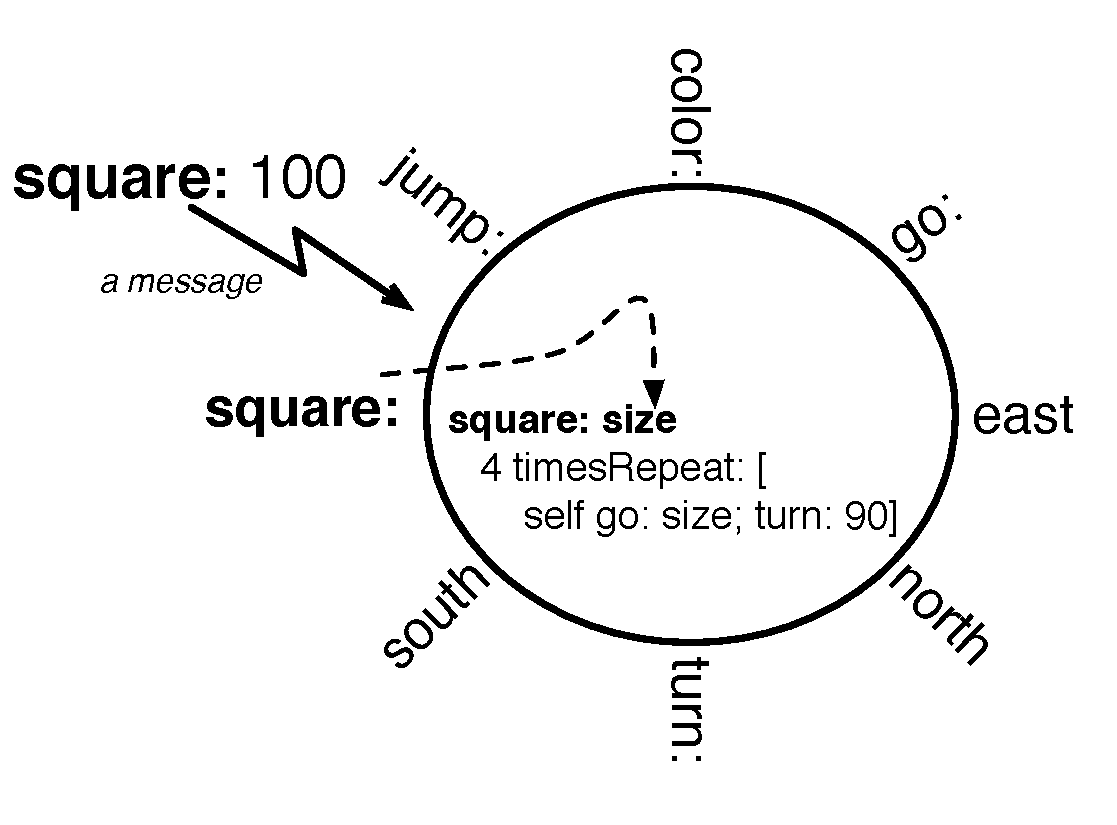
\includegraphics[width=0.5\textwidth]{/Users/ducasse/Workspace/FirstCircle/MyBooks/Bk-Writing/PharoBooks/LearningOOPWithPharoTrans/_result/pdf/Chapters/OOPNutshell/figures/basicMessageMethod.pdf}\caption{An object presents to the other objects an interface composed of a set of messages defining \textit{what} he can do. This behavior is realized by methods that specify \textit{how} the behavior is implemented. When a message is sent to an object a method with the message name (called selector) is looked up and executed. \label{basicMessageMethod}}\end{center}
\end{figure}


\begin{coffee}
An object is an entity that once created receives messages and performs some actions in reaction. When a message is sent to an object, a method with the message name is looked up and executed.
\end{coffee}
\section{An object is a protective entity}
An object is responsible of the way it realizes its reaction to a message.  It \textit{offers services} but \textit{hides} the way they are implemented (see Figure \ref{fig:encapsulationAtWork2}). We do not have to know how the method associated with the message selector is implemented.  Only the object knows the exact definition of the method.  This is when we define the method \textcode{square:} that defines how a turtle draws a square of a given size, that we focus on \textit{how} a turtle draws a square. Figure \ref{fig:encapsulationAtWork2} shows the message and the method \textcode{square:}. The method \textcode{square:} defines how to draw step by step a square, however the object only offers the message square: and does not show it implementation.

\begin{important}
An object presents to the other objects an \textit{interface} (i.e., a set of messages) defining \textit{what} the object can do. This behavior is realized by methods that specify \textit{how} the behavior is implemented. To perform something useful some data are most of the time required. Data are only accessed by the methods.
\end{important}

From a turtle \textit{user} point of view, the only relevant information is that the turtle effectively receiving the message \textcode{square:} executes the method that draws a square. So changing the definition of the \textcode{square:} method  to the one below does not have any consequence on the methods that call it. Figure \ref{fig:encapsulationAtWork2} illustrates this point.

\begin{displaycode}{plain}
square: s
   "Make the receiver draw a square of size s"

   self go: s; turn: 90; go: s; turn: 90.
   self go: s; turn: 90; go: s; turn: 90
\end{displaycode}


\begin{figure}

\begin{center}
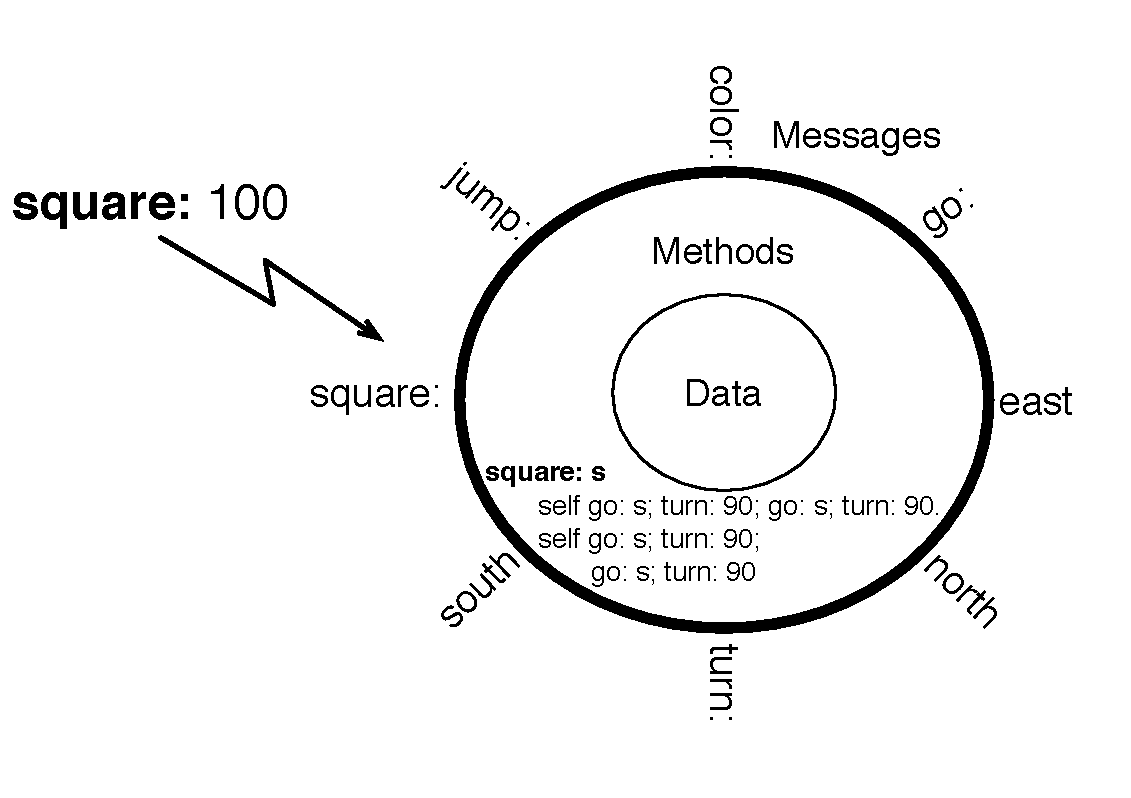
\includegraphics[width=0.5\textwidth]{/Users/ducasse/Workspace/FirstCircle/MyBooks/Bk-Writing/PharoBooks/LearningOOPWithPharoTrans/_result/pdf/Chapters/OOPNutshell/figures/encapsulationAtWork2.pdf}\caption{The message \textcode{square:} can be implemented differently. This different implementation does not impact the sender of the message who is not concerned by the internals of the object.\label{fig:encapsulationAtWork2}}\end{center}
\end{figure}


Hiding the internal representation is not limited to object-oriented programming but it is central to object-oriented programming. 

\begin{important}
An object is responsible of the way it realizes its reaction to a message. It offers services and hides the way they are implemented.
\end{important}
\section{An object protects its data}
An object holds some \textit{private data} that represents its state (see Figure \ref{fig:objectOne}). Moreover, it controls its state and should not let other objects play directly with them because this could let him into an inconsistent state.  For example, you do not want to somebody else plays with the data of your bank account directly and really want to control your transaction.

For example, a LOGO turtle can be represented by a position, a direction and a way to indicate if its pen is up or down. But, we cannot directly access these data and change them. For that we have to use the set of messages proposed by a turtle. These methods constitute the \textit{interface} of an object. We say that the object state is \textit{encapsulated}, this means that not everybody can access it. In fact, object-oriented programming is based on encapsulation, i.e., the fact that per default objects are the only ones that can access their own state.


\begin{figure}

\begin{center}
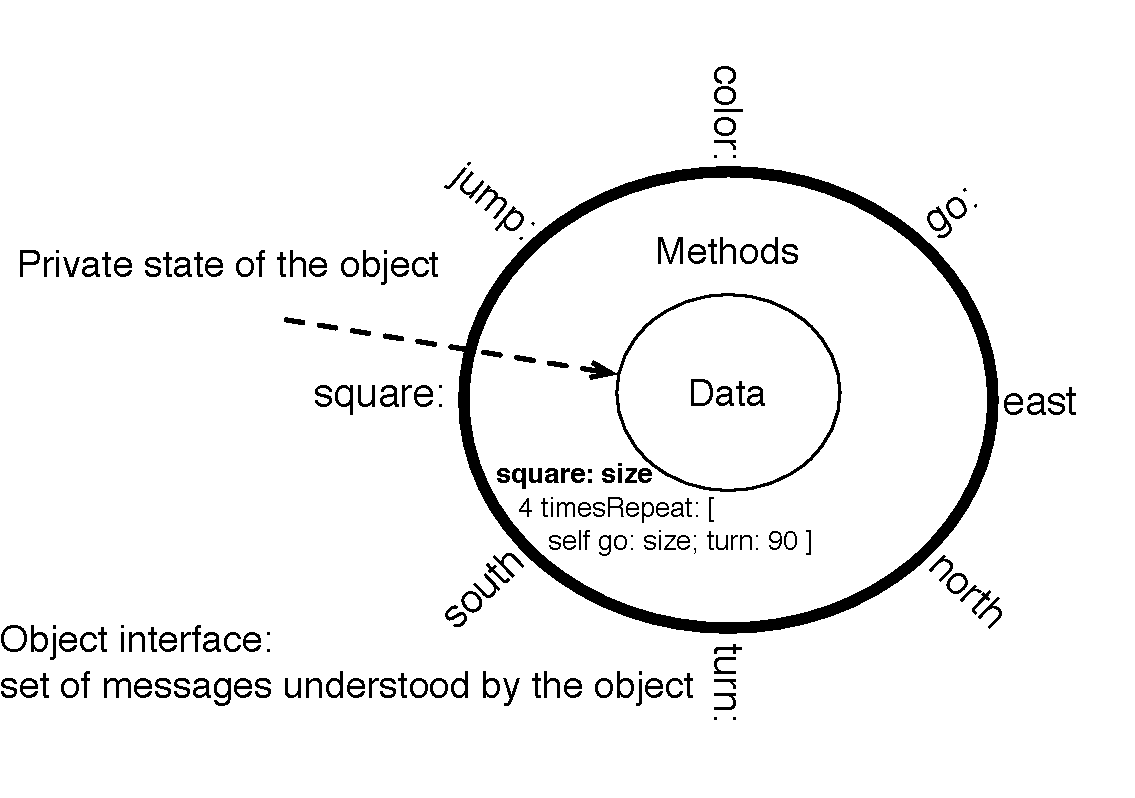
\includegraphics[width=0.45\textwidth]{/Users/ducasse/Workspace/FirstCircle/MyBooks/Bk-Writing/PharoBooks/LearningOOPWithPharoTrans/_result/pdf/Chapters/OOPNutshell/figures/privateData.pdf}\caption{A turtle is an object which has an interface, i.e., a set of messages to which it can reply and a private state that only its methods can access.\label{fig:objectOne}}\end{center}
\end{figure}


In Pharo, a client cannot access the state of an object if the object does not define a method to access it.  Moreover, clients should not  rely on the internal representation of an object because an object is free to change the way it  implements its behavior. Exposing the internal state of an object by defining methods providing access to the object data weakens the control that an object has over its own state.


\begin{figure}

\begin{center}
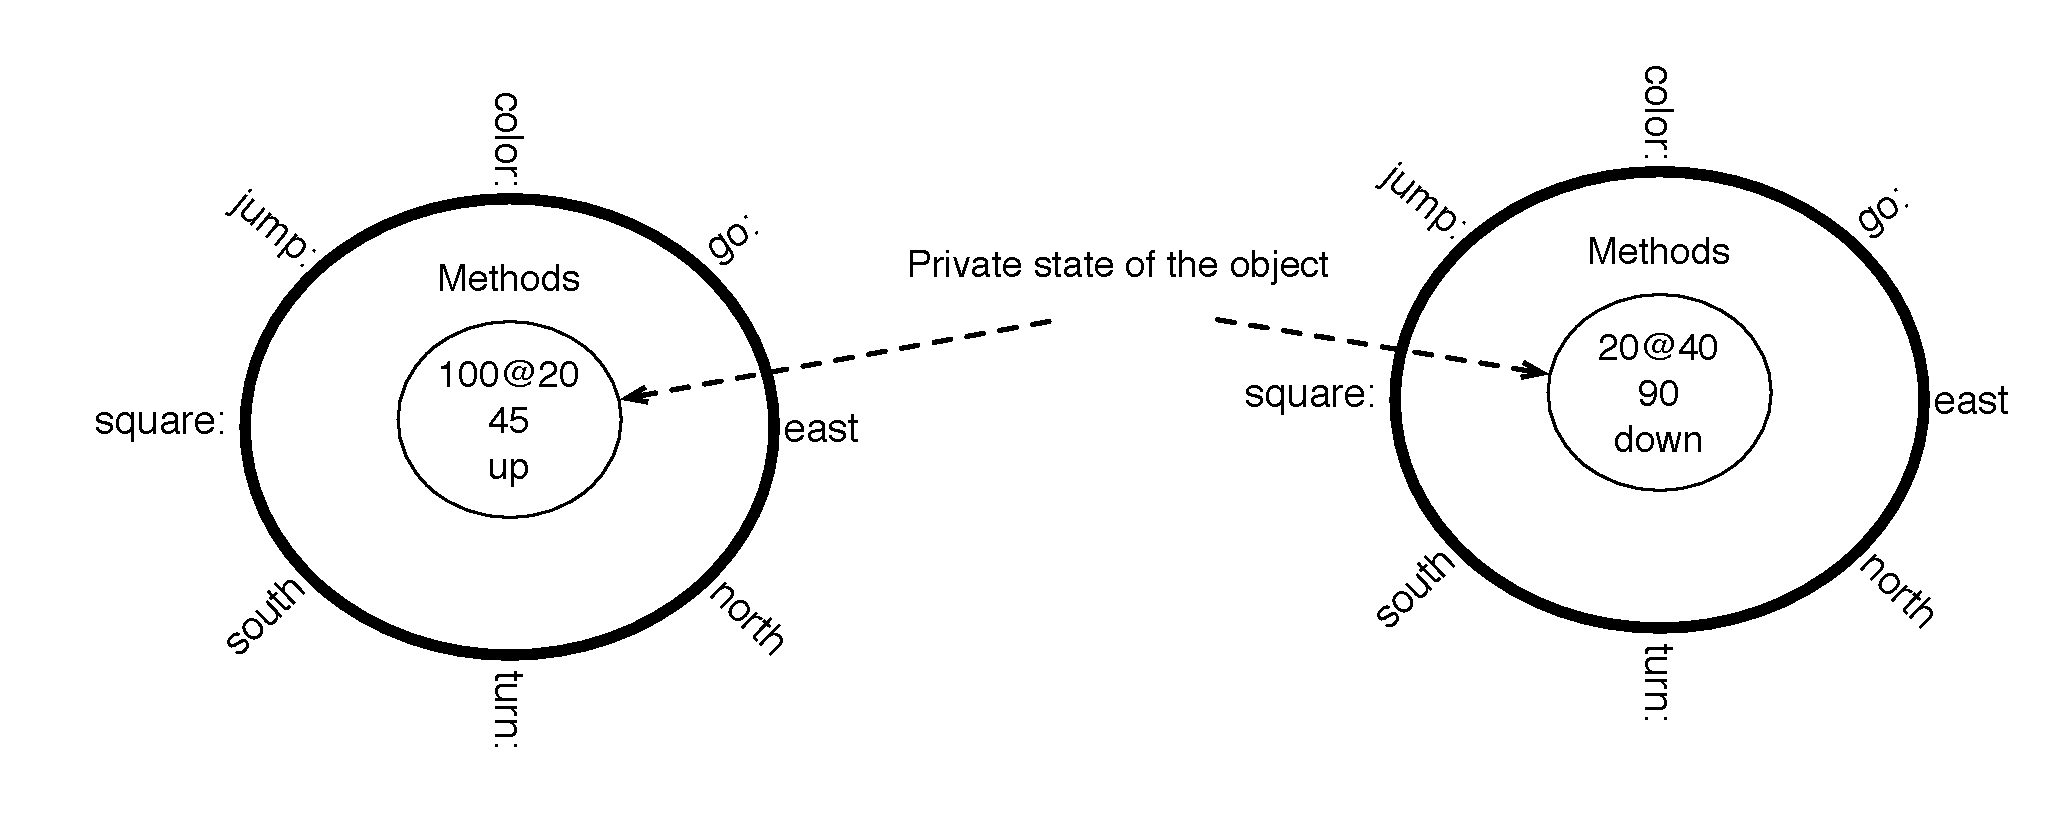
\includegraphics[width=0.7\textwidth]{/Users/ducasse/Workspace/FirstCircle/MyBooks/Bk-Writing/PharoBooks/LearningOOPWithPharoTrans/_result/pdf/Chapters/OOPNutshell/figures/privateDataTwoInstances.pdf}\caption{Two turtles have the same interface, i.e., set of messages  being understood but they have \textit{different} private state representing their  direction, position and pen status.\label{fig:twoInstances}}\end{center}
\end{figure}


\begin{important}
An object holds some \textit{private} data that represents its \textit{internal} state. Each object has its own state. Two objects of the same class share the same \textit{interface} but have their own private state.
\end{important}
\section{With counters}
Now that you got the main point of objects, we can see that it applies to everything. In Pharo \textit{everything} is an object. In fact there is \textit{nothing} else, only objects. Here is a little program with counters. 

We create two counters that we store in variables \textcode{c1} and \textcode{c2} instances of the class \textcode{Counter}. Each counter has its own state but exhibits the same behavior as all the counters defined by the class \textcode{Counter}: 

\begin{itemize}
\item when responding to the message \textcode{count}, it returns its value,
\item when responding to the message \textcode{increment}, it increment one to its current value. 
\end{itemize}

\begin{displaycode}{plain}
| c1 c2 |
c1 := Counter new.
c2 := Counter new.
c1 count.
>>> 0
c1 increment.
c1 increment.
c1 count. 
>>> 2
c2 count.
>>> 0
c 2 increment.
c2 count. 
>>> 1
\end{displaycode}
\section{A class: blueprint or factory of objects}
A class is a mold or cast of objects. A class specifies two important aspects of their instances:

\begin{itemize}
\item Instance \textbf{structure}. All the instances of a class will have the same structure expressed in terms of \textit{instance variables}. Pay attention that the variables are the same for all the instances of a class but not their values. Each instance has specific values for its instance variables.
\item Instance \textbf{behavior}. All the instances share the same behavior even if this one can be different because applied on different values. 
\end{itemize}

\begin{important}
A class is as a blueprint for its instances. It is a factory of objects. All objects will have the same structure and share a common behavior. 
\end{important}

Let us illustrate this with the class \textcode{Counter}.
\subsection{Object structure}
Let us study the \textcode{Counter} class definition.  

\begin{displaycode}{plain}
Object subclass: #Counter
	instanceVariableNames: 'count'
	classVariableNames: ''
	package: 'LOOP'
\end{displaycode}

The expresion \textcode{Object subclass: \#Counter} indicates that the class \textcode{Counter} is a subclass of the class \textcode{Object}.
It means that counter instances understand the messages defined also by the class \textcode{Object}. In Pharo, classes should at least be a subclass of the class \textcode{Object}. You will learn more about subclassing and inheritance in Chapter \ref{cha:inheritance}.

Then the class \textcode{Counter} defines that all the instances will have one instance variable named \textcode{count} using the expression \textcode{instanceVariableNames: 'count'}. And each instance of the class \textcode{Counter} will have a \textcode{count} variable with a \textit{different} value as we showed in the examples above.

Finally the class is defined in the package \textcode{'LOOP'}. A package is a kind of folder containing multiple classes. 
\subsection{Object behavior}
In addition a class is the place that groups the behavior of its instances. Indeed since all the instances of the class share the \textit{same} behavior definitions, such behavior is defined and grouped in a class.

For counters, the class defines how to retrieve the counter value, how to increment 
and decrement the count as used in the messages in the previous code snippets.

Here is the definition of the \textbf{method} \textcode{increment}. 
It simply adds one to the instance variable \textcode{count}.

\begin{displaycode}{plain}
Counter >> increment
	count := count + 1
\end{displaycode}

When we send a message to a counter for example in the expression \textcode{c1 increment}, 
the method \textcode{increment} will be applied on \textit{that} specific object \textcode{c1}.
In the expression \textcode{c1 increment}, \textcode{c1} is called the \textbf{receiver} of the message \textcode{increment}. 

In the method \textcode{increment},  the variable \textcode{count} refers to the variable of the \textbf{receiver} of the message. 

\begin{coffee}
A class defines methods that specify the behavior of all the instances created by the class.
\end{coffee}

Multiple methods can accessed to the instance variables of the receiver. For example the methods \textcode{increment}, \textcode{count:} \textcode{decrement} and \textcode{printOn:} all access the instance variable \textcode{count} of the receiver to perform different computation. 

\begin{displaycode}{plain}
Counter >> count: anInteger
	count := anInteger
\end{displaycode}

\begin{displaycode}{plain}
Counter >> decrement
	count := count - 1
\end{displaycode}

\begin{displaycode}{plain}
Counter >> printOn: aStream
   super printOn: aStream.
   aStream nextPutAll: ' with value: ', self count printString.
\end{displaycode}

For example, once the following program is executed the count  instance variable of the counter \textcode{c2} will hold the value 11, since the method \textcode{count:} will set its value to 10, and \textcode{increment} will set it to 11 and 12 and finally \textcode{decrement} will set it to 11. 

\begin{displaycode}{plain}
| c2 |
c2 := Counter new.
c2 count: 10.
c2 increment.
c2 increment.
c2 decrement.
\end{displaycode}
\subsection{Self is the message receiver}
Imagine that now we would like to send a message to the object that receives the message itself. We need a way to refer to this object. Pharo defines a special variable for this exact purpose: \textcode{self}. 

\begin{important}
\textcode{self} always refers to the message receiver that is currently executed.
\end{important}

For example we can implement the method \textcode{incrementByTwo} as follows:

\begin{displaycode}{plain}
Counter >> incrementByTwo
	self increment. 
	self increment
\end{displaycode}

When we execute the expression \textcode{c1 incrementByTwo}, during the execution of the method \textcode{incrementByTwo}, \textcode{self} refers to \textcode{c1}. 

We will explain  how a method is found when a message is sent but first we should explain inheritance, i.e., how a class is defined incrementally from a root class and all this will be explained  in Chapter \ref{cha:inheritance}.
\section{Class and instances are really different}
Classes and objects are different objects; they understand different messages. 

For example, sending \textcode{new} to the \textcode{Counter} class returns a newly created counter, while sending \textcode{new} to a counter results in an error. In the opposite way, sending \textcode{increment} to the class \textcode{Counter} leads also to an error because the class \textcode{Counter} is a factory of objects not the objects themselves. 

A class is a factory of objects. A class creates instances. An instance does not create other instances of the class.

\begin{coffee}
A class describes the structure (instance variables) and the behavior (methods) of \textit{all} its instances. The state of an instance is the value of its instance variables and it is specific to one single object while the behavior is shared by all the instances of a class.
\end{coffee}
\section{Conclusion}
In this chapter you saw that: 

\begin{itemize}
\item An object is a computer entity that once created receives messages and performs some actions in reaction.
\item An object has an unique identity.
\item An object holds some private data that represent its internal state.
\end{itemize}

\begin{itemize}
\item A class is a factory of objects: It \textit{describes} the internal structure of all its instances by means of instance variable. 
\item All objects of the same class share the same behavior, i.e., the same method definitions.
\item Instance variables are accessible by all the methods of a class. Instance variables have the same lifetime than the object to which they belong to.
\item In Pharo , instance variables cannot be accessed from outside of an object. Instance variables are only accessible from the methods of the class that define them.
\item Methods define the behavior of all the instances  of the class they belong to.
\end{itemize}
\chapter{Revisiting objects and classes}
In the previous chapter we presented objects and classes via simple examples. In this chapter we introduce a little bit more elaborated example: a little file system where we revisit everything and extend it to explain \textit{late binding}, \textit{distribution of responsibilities} and \textit{delegation}. The file example will be extended to present \textit{inheritance} in Chapter \ref{cha:inheritance}.
\section{A simple and naive file system}
We start to present a simple example that we use to present and explain the concepts: a simple and naive file system as shown in Figure \ref{figdirectories}. 
What the diagram shows is that we have:

\begin{itemize}
\item files that also have a name and a contents. Here we get three different files \textcode{Babar}, \textcode{Astroboy} and \textcode{tintinEtLesPicaros}.
\item directories that have a name and can contain other files or directories. Here we get the \textcode{manga}, \textcode{comics}, \textcode{oldcomics} and \textcode{belgiumSchool} directories. Directories can be nested: \textcode{comics} contains three repositories. The \textcode{belgiumSchool} directory contains \textcode{tintinEtLesPicaros}. 
\end{itemize}


\begin{figure}

\begin{center}
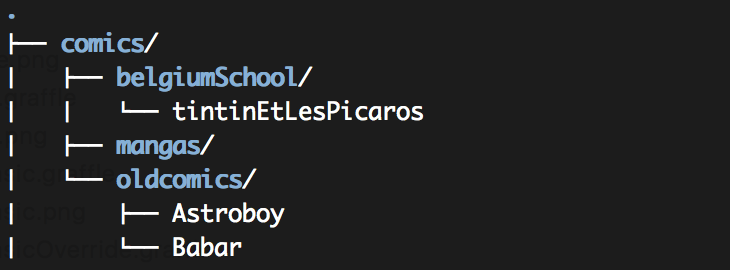
\includegraphics[width=0.5\textwidth]{/Users/ducasse/Workspace/FirstCircle/MyBooks/Bk-Writing/PharoBooks/LearningOOPWithPharoTrans/_result/pdf/Chapters/OOPNutshell/figures/comicsFileTree.png}\caption{Some directories and files organised in a file system.\label{figdirectories}}\end{center}
\end{figure}

\section{Studying a first scenario}
Since what we want to develop may be a bit unclear for us, let us define first an example. In the rest of this book we will code such examples as tests that can automatically be executed. For now it would make the discourse too complex, so we just use little code examples. 

We create two directories.

\begin{displaycode}{plain}
| dComics dOldComics dManga |
dComics := MFDirectory new name: 'comics'.
dOldComics := MFDirectory new name: 'oldcomics'.
\end{displaycode}

We add the oldcomics folder to comics and we check that the parent children relationship is well set. 

\begin{displaycode}{plain}
	...
dComics addElement: dOldComics. 
dOldComics parent == dComics
>>> true
\end{displaycode}

Here we verify that the parent of \textcode{dOldComics} is \textcode{dComics}: the message \textcode{ == } checks that the receiver is the same object than the argument.  

You can also inspect the receiver as follows and if you click on the instance variable parent of the receiver you should obtain the situation depicted by Figure \ref{inspectingComics}.

\begin{displaycode}{plain}
	...
dOldComics inspect
\end{displaycode}


\begin{figure}

\begin{center}
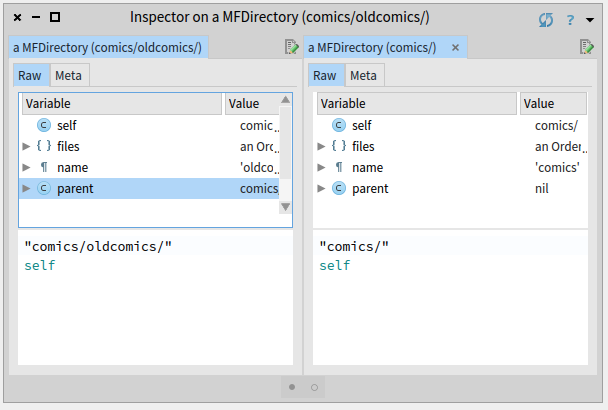
\includegraphics[width=0.7\textwidth]{/Users/ducasse/Workspace/FirstCircle/MyBooks/Bk-Writing/PharoBooks/LearningOOPWithPharoTrans/_result/pdf/Chapters/OOPNutshell/figures/inspectingComics.png}\caption{Inspecting \textcode{dOldComics} and clicking on the \textcode{parent} variable. \label{inspectingComics}}\end{center}
\end{figure}


We continue with some queries.

\begin{displaycode}{plain}
	...
dComics parent
>>> nil
\end{displaycode}

Here we verify that \textcode{dOldComics} is comprised in the children of \textcode{dComics}. 

\begin{displaycode}{plain}
	...
dComics children includes: dOldComics. 
>>> true
\end{displaycode}

We create a new repository and we check that once added to a parent repository, it is included in the 
children.

\begin{displaycode}{plain}
dManga := MFDirectory new name: 'manga'.
dComics addElement: dManga. 
dComics children includes: dManga
>>> true
\end{displaycode}


\begin{figure}

\begin{center}
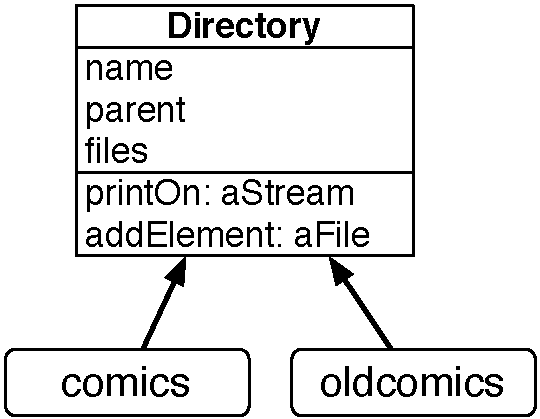
\includegraphics[width=0.35\textwidth]{/Users/ducasse/Workspace/FirstCircle/MyBooks/Bk-Writing/PharoBooks/LearningOOPWithPharoTrans/_result/pdf/Chapters/OOPNutshell/figures/DirectoryAndInstancesV0.pdf}\caption{The \textcode{Directory} class and some instances (directories).\label{directories}}\end{center}
\end{figure}

\section{Defining a class}
Let us start by defining the directory class. 

\begin{displaycode}{plain}
Object subclass: #MFDirectory
	instanceVariableNames: 'parent name files'
	classVariableNames: ''
	package: 'MyFS'
\end{displaycode}

When we create a directory, its files is an empty ordered collection. This is what we express in the following method \textcode{initialize}.

\begin{displaycode}{plain}
MFDirectory >> initialize
	files := OrderedCollection new
\end{displaycode}

A newly created object is sent the message \textcode{initialize} just after its creation. Therefore the \textcode{initialize} method is executed. 

Now we can write the method \textcode{addElement:}. 
(To keep things simple, note that we consider that when a file is added to a directory, it was not belonging to a another directory. This behavior could be implemented by \textcode{aFile moveTo: aDirectory})
Adding a file to a directory means: (1) that the parent of the file is changed to be the directory to which it is added, (2) that the added file is added to the list of files contained in the directory.

\begin{displaycode}{plain}
MFDirectory >> addElement: aFile
	aFile parent: self. 
	files add: aFile
\end{displaycode}

Note that the method name \textcode{addElement:} is not nice but we chose it on purpose so that you do not believe that delegating
requires that the methods have the same name. An object can delegate its part of duties to another object by simply passing a message. 

We should then define the methods \textcode{name:}, \textcode{parent:}, \textcode{parent}, and \textcode{children} to be able to run our example.

\begin{displaycode}{plain}
MFDirectory >> name: aString
	name := aString
\end{displaycode}

\begin{displaycode}{plain}
MFDirectory >> parent: aFile
	parent := aFile
\end{displaycode}

\begin{displaycode}{plain}
MFDirectory >> parent
	^ parent
\end{displaycode}

\begin{displaycode}{plain}
MFDirectory >> children
	^ files
\end{displaycode}

With such method definitions, our little example should run. It should not print the same results because we did not change the printing of the objects yet. 
\subsection{A first little analysis}
When we look at the implementation of the method to add a file to a directory we see that the class \textcode{MFDirectory} used another class \textcode{OrderedCollection} to store the information about the files it contains. An ordered collection is a quite complex object: it can insert, remove elements, grow its size, and many more operations. 

We say that the class \textcode{MFDirectory} delegates a part of its duties (to keep the information of the files it contains) to the class \textcode{OrderedCollection}. In addition, when an object is executed, the object to which it may delegate part of its computation may change dynamically. 

Such behavior is not specific to object-oriented programming, in procedural languages we can call another function defined on a data structure. 
Now with object-oriented programming, there is a really important point: an object will send messages to other objects (even from the same class) and such message send will use the message offered by the receiver. There is normally no way for an object to access the internal structure of another object.
\section{Printing a directory}
Now we would like to get the directory printed in a better way. Without too much explanation, you should know that the method \textcode{printOn: astream} of an object is executed when the system or we send the message \textcode{printString} to an object. So we can specialise it. 

The argument passed to the method \textcode{printOn:} is a stream. A stream is an object in which we can store information one after the other in sequence using the message \textcode{\textless{}\textless{}}. The argument of \textcode{\textless{}\textless{}} should be a sequence of objects such as string (which is a sequence of characters).

\begin{displaycode}{plain}
MFDirectory >> printOn: aStream
	aStream << name
\end{displaycode}

Let us try. 

\begin{displaycode}{plain}
| el1 el2 |
el1 := MFDirectory new name: 'comics'.
el2 := MFDirectory new name: 'oldcomics'.
el1 addElement: el2.
el1 printString
>>> 'comics'
\end{displaycode}

\begin{displaycode}{plain}
	...
el2 printString
>>> 'oldcomics'
\end{displaycode}

What would be nice is to get the full path so that we can immediately understand the configuration.
For example we would like to  finish with a '/' to indicate that this is a directory as with the ls command on unix. 

\begin{displaycode}{plain}
| el1 el2 |
el1 := MFDirectory new name: 'comics'.
el2 := MFDirectory new name: 'oldcomics'.
el1 addElement: el2.
el1 >> printString.
>>>'comics'
\end{displaycode}

\begin{displaycode}{plain}
	...
el2 printString
>>> 'comics/oldcomics/'
\end{displaycode}

A possible definition is the following one:

\begin{displaycode}{plain}
MFDirectory >> printOn: aStream
	parent isNil 
		ifFalse: [ parent printOn: aStream ].
	aStream << name.
	aStream << '/'
\end{displaycode}


\begin{figure}

\begin{center}
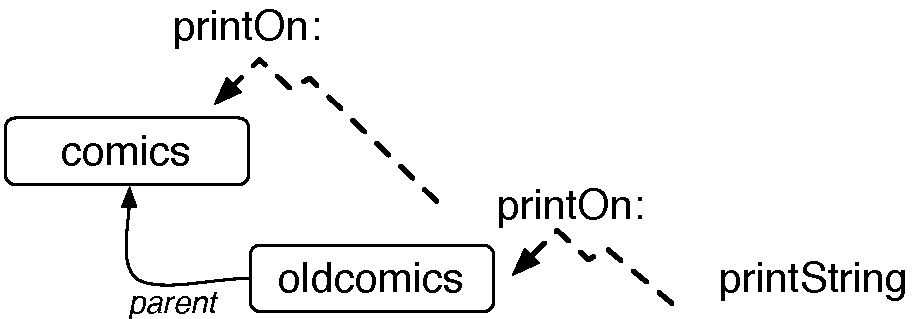
\includegraphics[width=0.55\textwidth]{/Users/ducasse/Workspace/FirstCircle/MyBooks/Bk-Writing/PharoBooks/LearningOOPWithPharoTrans/_result/pdf/Chapters/OOPNutshell/figures/InstancesRecursion.pdf}\caption{Navigating an object graph by sending message to different objects. \label{InstancesRecursion}}\end{center}
\end{figure}


Try it and it should print the expected results.
What do we see with this definition: it is a kind of recursive definition. The name of a directory is in fact the concatenation (here we just add in the stream but this is the same. ) of the name of its parents (as shown in Figure \ref{InstancesRecursion}).
Similar to a recursive function navigating a structure composed of similar elements (like a linked-list or any structure defined by induction), each parent receives and executes another time the \textcode{printOn:} method and returns the name for its part.
\section{Adding files}
Now we want to add files. Once we will have defined files we will be able to have a graph of objects of different kinds represent our file system with directories and files as shown in Figure \ref{Instances}.


\begin{figure}

\begin{center}
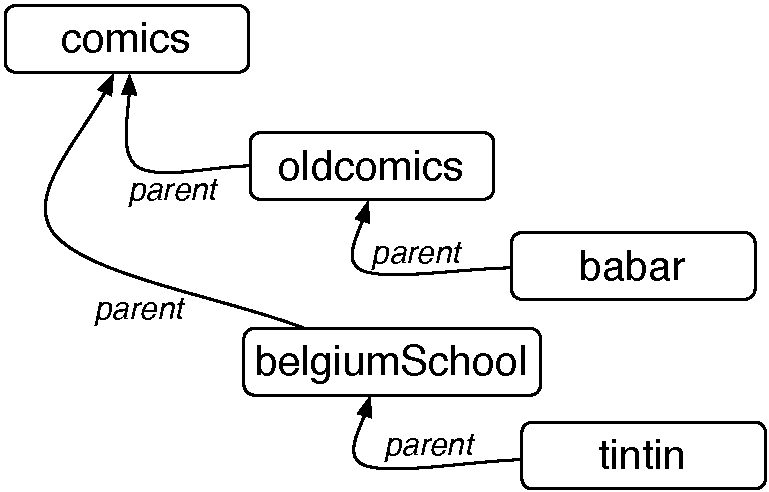
\includegraphics[width=0.45\textwidth]{/Users/ducasse/Workspace/FirstCircle/MyBooks/Bk-Writing/PharoBooks/LearningOOPWithPharoTrans/_result/pdf/Chapters/OOPNutshell/figures/Instances.pdf}\caption{A graph of objects to represent our file system. \label{Instances}}\end{center}
\end{figure}

\subsection{An example first}
Again let us start with an example.  A file should contain some contents. 

\begin{displaycode}{plain}
| el1 dOldComics |
el1 := MFFile new name: 'astroboy'; contents: 'The story of a boy turned into a robot that saved the world'.
dOldComics := MFDirectory new name: 'oldcomics'.
dOldComics addElement: el1. 
el1 printString.
>>>
'oldcomics/astroboy'
\end{displaycode}


\begin{figure}

\begin{center}
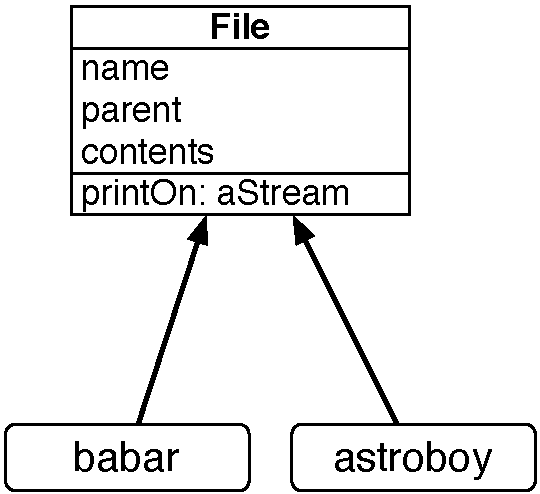
\includegraphics[width=0.35\textwidth]{/Users/ducasse/Workspace/FirstCircle/MyBooks/Bk-Writing/PharoBooks/LearningOOPWithPharoTrans/_result/pdf/Chapters/OOPNutshell/figures/FileV0.pdf}\caption{A new class and its instances.\label{FileV0}}\end{center}
\end{figure}

\subsection{A new class definition}
Again a file needs a name, a parent and in addition a contents.

We define the class \textcode{MFFile} as follows and illustrated in Figure \ref{FileV0}.
Note that this solution is not satisfactory and we will propose a much better one later.

\begin{displaycode}{plain}
Object subclass: #MFFile
	instanceVariableNames: 'parent name contents'
	classVariableNames: ''
	package: 'MyFS'
\end{displaycode}

As for the directories we initialize the contents of a file with a default value. 

\begin{displaycode}{plain}
MFFile >> initialize
	contents := ''
\end{displaycode}

We should define the same methods for \textcode{parent:}, \textcode{parent} and \textcode{name:}. This duplication coupled with the fact that we get nearly the same class definition should be a clear warning. It means that we do not reuse enough and that if we want to change the system we will have to change it multiple times and we may introduce errors by forgetting one place. 
We will address it in Chapter \ref{cha:inheritance}. In addition we will add a method to be able to set the contents of the file \textcode{contents:}.

\begin{displaycode}{plain}
MFFile >> name: aString
	name := aString
\end{displaycode}

\begin{displaycode}{plain}
MFFile >> parent: aFile
	parent := aFile
\end{displaycode}

\begin{displaycode}{plain}
MFFile >> parent
	^ parent
\end{displaycode}

\begin{displaycode}{plain}
MFFile >> contents: aString
	contents := aString
\end{displaycode}

At the stage we should be able to define a file and adding it to a directory.

Now we should redefine the implementation of \textcode{printOn:} to print nicely the name of file:

\begin{displaycode}{plain}
MFFile >> printOn: aStream
	aStream << name
\end{displaycode}

But this is not enough because we will just get \textcode{'astroboy'} and not \textcode{'oldcomics/astroboy'}.
So let us improve it.

\begin{displaycode}{plain}
MFFile >> printOn: aStream
	parent isNil ifFalse: [ 
		parent printOn: aStream ].
	aStream << name
\end{displaycode}


\begin{figure}

\begin{center}
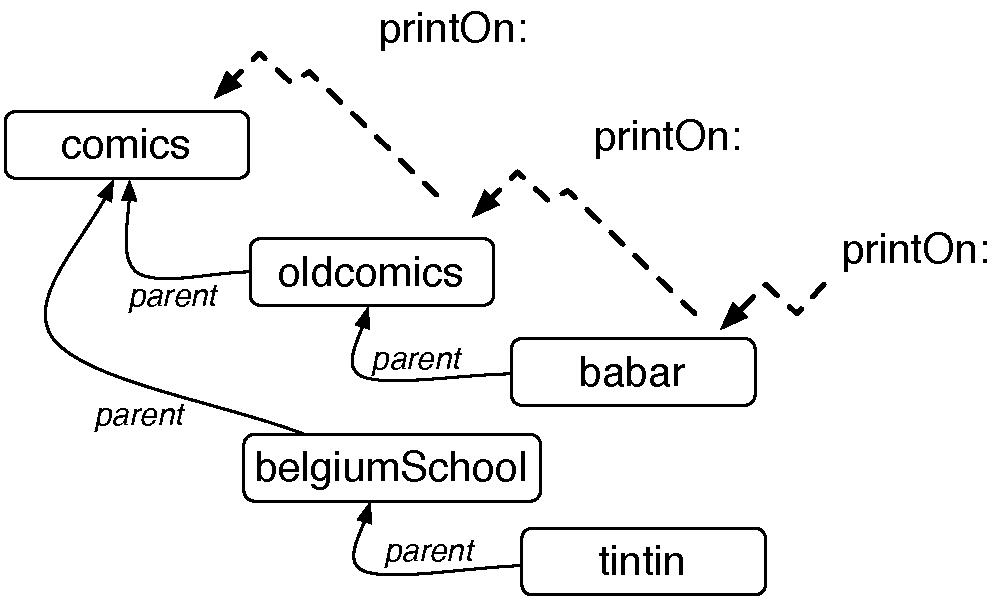
\includegraphics[width=0.6\textwidth]{/Users/ducasse/Workspace/FirstCircle/MyBooks/Bk-Writing/PharoBooks/LearningOOPWithPharoTrans/_result/pdf/Chapters/OOPNutshell/figures/InstancesRecursion2.pdf}\caption{Printing a file: Sending messages inside a graph of different objects. \label{InstancesRecursion2}}\end{center}
\end{figure}

\section{One message and multiple methods}
Before continuing let us step back and analyse the situation. We send the same messages and we execute different methods. 

\begin{displaycode}{plain}
| el1 dOldComics dComics |
el1 := MFFile new name: 'astroboy'; contents: 'The story of a boy turned into a robot that saved the world'.
dOldComics := MFDirectory new name: 'oldcomics'.
dComics := MFDirectory new name: 'comics'.
dComics addElement: dOldComics.
dOldComics addElement: el1. 
el1 printString.
>>>
'comics/oldcomics/astroboy'
\end{displaycode}

\begin{displaycode}{plain}
dOldComics printString.
>>>
'comics/oldcomics/'
\end{displaycode}

What we see is that there is one message and several implementations of methods and that sending a message will find and execute the correct method. For example, there are two methods \textcode{printOn:} one for file and one for directory but only one message \textcode{printOn:} sent from the \textcode{printString} message.

In addition a method can be defined in terms of messages sent to other objects. The method \textcode{printOn:} for directories is complex and it delegates the same message to other objects, its parents (as illustrated by Figure \ref{InstancesRecursion2}). The method \textcode{addElement:} delegates to the OrderedCollection sending a different message \textcode{add:}.
\section{Objects: stepping back}
Now that we saw some examples of objects, it is time to step back. Objects are defined by the values of their state, their behavior (shared with the other instances of their class) and an identity. 

\begin{itemize}
\item \textbf{State.} Each object has specific values. While all the instances of classes have the same structure, each instance has its own values. Each object has a private state. Clients or users of an object cannot access the state of the object if this one does not explicitly expose it by defining a method returning it (such as the message \textcode{count}).
\item \textbf{Behavior.} Each object shares the same behavior with all the instances of its class.
\item \textbf{Identity.} An object has an identity. It is unique. \textcode{oldcomics} is clearly not the same as \textcode{comics}.
\end{itemize}
\section{Examples of distribution of responsibilities }
We will now implement two functionalities: the size of directories and a search based on the contents of the files. This will set the context to explain the key concept of distribution of responsibilities.


\begin{figure}

\begin{center}
\includegraphics[width=0.6\textwidth]{/Users/ducasse/Workspace/FirstCircle/MyBooks/Bk-Writing/PharoBooks/LearningOOPWithPharoTrans/_result/pdf/Chapters/OOPNutshell/figures/FileDirectoryV1.pdf}\caption{Two classes understanding similar sets of message.\label{NutFileDirectoryV1}}\end{center}
\end{figure}

\subsection{File size }
Let us imagine that we want to compute the size of a directory. Note that the size computation we propose is fantasist but this is for the sake of the example. To perform such a computation we should also define what is the size of a file. Again let us start with examples (that you will turn into tests in the future.).

First we define the file size as the size of its name plus the size of its contents.

\begin{displaycode}{plain}
| el |
el := MFFile new name: 'babar'; contents: 'Babar et Celeste'.
el size = 'babar' size + 'Babar et Celeste' size.
>>> true
\end{displaycode}

Second we define the directory size as its name size plus the size of its files and we add and arbitrary number: 2. 

\begin{displaycode}{plain}
| p2 el |
el := MFFile new name: 'babar'.
p2 := MFDirectory new name: 'oldcomics'.
p2 addElement: el. 
p2 size = 'oldcomics' size + 'babar' size + 2
>>> true
\end{displaycode}

We define two methods \textcode{size} one for each class (see Figure \ref{NutFileDirectoryV1}).

\begin{displaycode}{plain}
MFFile >> size
	^ contents size + name size
\end{displaycode}

\begin{displaycode}{plain}
MFDirectory >> size
	| sum |
	sum := 0.
	files do: [ :each | sum := sum + each size ].
	sum := sum + name size.
	sum := sum + 2.
	^ sum
\end{displaycode}
\subsection{Search }
Let us imagine that we want to search the files matching a given string. 
Here is an example to set the stage.

\begin{displaycode}{plain}
| p el1 el2 |
p := MFDirectory new name: 'comics'.
el1 := MFFile new name: 'babar'; contents: 'Babar et Celeste'.
p addElement: el1.
el2 := MFFile new name: 'astroboy'; contents: 'super cool robot'.
p addElement: el2.
(p search: 'Ba') includes: el1
>>> true
\end{displaycode}

To implement this behavior is quite simple: we define two methods one in each class (as shown in Figure \ref{NutFileDirectoryV1}).

\begin{displaycode}{plain}
MFFile >> search: aString
	^ '*', aString, '*' match: contents
\end{displaycode}

\begin{displaycode}{plain}
MFDirectory >> search: aString
	^ files select: [ :eachFile | eachFile search: aString ]
\end{displaycode}
\section{Important points}
These two examples show several \textit{important} points:
\subsection{Modular thinking}
Each method is modular in the sense that it only focuses on the behavior of the objects specified by the class defining the method. Such method can be built by sending other messages without having to know how such methods are defined.
It also means that we can add a new kind of classes or remove one without having to change the entire system.
\subsection{Sending a message is making a choice}
We send \textit{one} message and one method amongst the \textit{multiple} methods with the same name will be selected and executed. The method is dynamically looked up during execution as we will see in Chapters \ref{cha:inheritance} and \ref{cha:messages}. Sending a message is selecting the corresponding method having the same name than the message.  When a message is sent to an object the corresponding method is looked in the class of the message receiver.

\begin{important}
Sending a message is making a choice. The system selects for us the correct method to be executed.
\end{important}
\subsection{Polymorphic objects }
We created objects (files and directories) that are \textit{polymorphic} in the sense that they offer a common set of messages (\textcode{search:}, \textcode{printOn:}, \textcode{size}, \textcode{parent:}). This is really powerful because we can compose objects (for example add a new directory or a file) without changing the program. 
Imagine that we add a new kind of directories we can introduce it and reuse extending programs based on \textcode{size} or \textcode{search:} \textit{without} changing them. 

\begin{important}
Creating polymorphic objects is a really powerful capability. It lets us extend and change programs without breaking them. 
\end{important}

Most of the time it is better to give similar name to methods performing similar behavior, and different names when the methods are doing semantically different actions, so that users of the objects are not confused. 

The  polymorphism is really a strength of object-oriented languages because it allows one to treat different objects, i.e., instances of different classes, uniformly as soon as they implement the same messages. Polymorphism works in synergy with the idea that an object is responsible to decide how to react to message reception. Indeed, the fact that different objects can implement the same messages let us write code that only tell the objects to execute some actions without worrying exactly about the kind of objects. 
\section{Distribution of responsibilities}
This example as well as the printing of files and directories illustrates something fundamental in 
object-oriented programming: the distribution of responsibilities. With the distribution of responsibilities,  each kind of objects is responsible for a specific behavior and a more elaborated behavior is composed out of such different behavior. The size of a directory is computed based on the size of its files by requesting the files to compute their size. 
\subsection{Procedural}
Let us take some time to compare with procedural thinking. Computing the size of a list of files and directories would have been expressed as a monolitic behavior sketch below:

\begin{displaycode}{plain}
sizeOfFiles: files
	| sum | 
	sum := 0.
	files do: [ :aFile | 
		aFile class = MFFile
			ifTrue: [ sum := sum + aFile name size + aFile contents size ].
		aFile class = MFDirectory
			ifTrue: [ 
				| fileSum |
				fileSum := 0.
				each files do: [:anInsideFile | fileSum := fileSum + anInsideFile name size + anInsideFile contents size ].
				sum := sum + fileSum + each name size + 2].
	^ sum	
\end{displaycode}

While this example is a bit exagerated, we see several points:

\begin{itemize}
\item First, we explicitly check the kind of structures we are manipulating. If this is a file or directory we do something different.
\item Second, the logic of the computation is defined inside the \textcode{sizeOfFiles:} itself, and not in the entities themselves.   This means in particular that such logic cannot be reused.
\item A part of the implementation logic is exposed and not in control of the object. It means that if we decide to change the internal structure of our classes, we will have to change this function too.
\item Adding a new kind of such as a root directory is not modular. We will have to modify the method \textcode{sizeOfFiles:} function.
\end{itemize}

What you should also see when you compare the two versions is that in the procedural version we have to check the kind of object we manipulate. 
In the object-oriented version, we simply tell the object to perform its own computation and return the result to us. 

\begin{important}
Don't ask, tell. Object-oriented programming essence is about sending order not checking state.
\end{important}
\section{So far so good? Not fully!}
We have a system with two classes and it offers some behavior composed out of well defined local behavior (see Figure \ref{NutFileDirectoryV1}). We can have objects composed out of other objects and messages flow within the graph. Object-oriented programming could stop here. Now it is annoying to have to duplicate structure and some methods between files and directories and this is what we will see when we will look at inheritance in Chapter \ref{cha:inheritance}.
Inheritance is a mechanism to specialize incrementally classes from other classes. 
\section{Conclusion}
\begin{itemize}
\item A class describes the state (instance variables) and the behavior (methods) of all its instances. The state of an instance is the value of its instance variables and it is specific to one single object while the behavior is shared by all the instances of a class.
\item Different objects, instances of different classes, can react differently to the same messages.
\item When sending a message, the associated method is found and executed.
\end{itemize}
\chapter{Converter}\label{cha_converter}
In this chapter you will implement a little temperature converter between celsius and fahrenheit degrees. It is so simple that it will help us to get started with Pharo and also with test driven development. Near the end of the chapter we will add logging facilities to the converter so that we can log the temperatures of certain locations.  For this you will create a simple class and its tests. 

We will show how to write test to specify the expected results. Writing tests is really important. It is one important tenet of Agile Programming and Test Driven Development (TDD). We will explain later why this is really good to have tests. For now we just implement them. We will also discuss a bit a fundamental aspects of float comparison and we will also present some loops.
\section{First a test}
First we define a test class named \textcode{TemperatureConverterTest} within the package \textcode{MyConverter}. It inherits from the class \textcode{TestCase}. This class is special, any method starting with \textcode{'test'} will be executed automatically, one by one each time on a new instance of the class (to make sure that tests do not interfere with each others). 

\begin{displaycode}{plain}
TestCase subclass: #TemperatureConverterTest
	instanceVariableNames: ''
	classVariableNames: ''
	package: 'MyConverter'
\end{displaycode}

Converting from Fahrenheit to Celsius is done with a simple linear transformation.
The formula to get Fahrenheit from Celsius is F = C * 1.8 + 32. 
Let us write a test covering such transformation. 30 Celsius should be 86 Fahrenheit. 

\begin{displaycode}{plain}
testCelsiusToFahrenheit

	| converter |
	converter := TemperatureConverter new. 
	self assert: ((converter convertCelsius: 30) = 86.0)
\end{displaycode}

The test is structured the following way:

\begin{itemize}
\item Its selector starts with \textcode{test}, here the method is named \textcode{testCelsiusToFahrenheit}.
\item It creates a new instance of \textcode{TemperatureConverter} (it is called the \textit{context} of the test or more technically its fixture).
\item Then we check using the message \textcode{assert:} that the expected behavior is really happening. 
\end{itemize}

The message \textcode{assert:} expects a boolean. Here the expression \textcode{((converter convertCelsius: 30) = 86.0)} returns a boolean. \textcode{true} if the converter returns the value 86.0, \textcode{false} otherwise. 

The testing framework also offers some other similar methods. One is particularly interesting: \textcode{assert:equals:} makes the error reporting more user friendly. The previous method is strictly equivalent to the following one using \textcode{assert:equals:}. 

\begin{displaycode}{plain}
testCelsiusToFahrenheit

	| converter |
	converter := TemperatureConverter new. 
	self assert: (converter convertCelsius: 30) equals: 86.0
\end{displaycode}

The message \textcode{assert:equals:} expects an expression and a result. Here \textcode{(converter convertCelsius: 30)} and \textcode{86.0}. You can use the message you prefer and we suggest to use \textcode{assert:equals:} since it will help you to understand your mistake by saying: \textcode{'You expect 86.0 and I got 30'} instead of simply telling you that the result is \textcode{false}. 
\section{Define a test method (and more)}
While defining the method \textcode{testCelsiusToFahrenheit} using the class browser, the system will tell you that the class \textcode{TemperatureConverter} does not exist (This is true because we did not define it so far). The system will propose to create it. Just let the system do it. 

Once you are done. You should have two classes: \textcode{TemperatureConverterTest} and \textcode{TemperatureConverter}. As well as one method: \textcode{testCelsiusToFahrenheit}. The test does not pass since we did not implement the conversion method (as shown by the red color in the body of \textcode{testCelsiusToFahrenheit}).

Note that you entered the method above and the system compiled it. Now in this book we want to make sure that you know about which method we are talking about hence we will prefix the method definitions with their class. For example the method \textcode{testCelsiusToFahrenheit} in the class \textcode{TemperaturConverterTest} is defined as follows: 

\begin{displaycode}{plain}
TemperaturConverterTest >> testCelsiusToFahrenheit

	| converter |
	converter := TemperatureConverter new. 
	self assert: (converter convertCelsius: 30) equals: 86.0
\end{displaycode}
\section{The class TemperaturConverter}
The class \textcode{TemperaturConverter} is defined as shown below. You could have define it before defining the class  \textcode{TemperaturConverterTest} using the class definition below: 

\begin{displaycode}{plain}
Object subclass: #TemperatureConverter
	instanceVariableNames: ''
	classVariableNames: ''
	package: 'MyConverter'
\end{displaycode}

This definition in essence, says that:

\begin{itemize}
\item We want to define a new class named \textcode{TemperaturConverter}.
\item It has no instance or class variables (\textcode{''} means empty string).
\item It is packaged in package \textcode{MyConverter}.
\end{itemize}

Usually when doing Test Driven Development with Pharo, we focus on tests and lets the system propose us some definitions. Then we can define the method as follows.

\begin{displaycode}{plain}
TemperatureConverter >> convertCelsius: anInteger 
	"Convert anInteger from celsius to fahrenheit"
	
	^ ((anInteger * 1.8) + 32)
\end{displaycode}

The system may tell you that the method is an utility method since it does not use object state. 
It is a bit true because the converter is a \textit{really} simple object. For now do not care. 

Your test should pass. Click on the icon close to the test method to execute it.
\section{Converting from Farhenheit to Celsius }
Now you got the idea. Let us define a test for the conversion from Fahrenheit to Celsius. 

\begin{displaycode}{plain}
TemperatureConverterTest >> testFahrenheitToCelsius

	| converter |
	converter := TemperatureConverter new. 
	self assert: (converter convertFarhenheit: 86) equals: 30.0.
	self assert: (converter convertFarhenheit: 50) equals: 10
\end{displaycode}

Define the method \textcode{convertFarhenheit: anInteger}

\begin{displaycode}{plain}
TemperatureConverter >> convertFarhenheit: anInteger 
	"Convert anInteger from fahrenheit to celsius"
	
	... Your solution ...
\end{displaycode}

Run the tests they should all pass. 
\section{About floats}
The conversions method we wrote returns floats. Floats are special objects in computer science because it is complex to represent infinite information (such as all the numbers between two consecutive integers) with a finite space (numbers are often represented with a fixed number of bits). In particular we should pay attention when comparing 
two floats. Here is a surprising case: we add two floats and the sum is not equal to their sums. 

\begin{displaycode}{plain}
(0.1 + 0.2) = 0.3
> false
\end{displaycode}

This is because the sum is not just equal to \textcode{0.3}. The sum is in fact the number  \textcode{0.30000000000000004}

\begin{displaycode}{plain}
(0.1 + 0.2)
> 0.30000000000000004
\end{displaycode}

To solve this problem in Pharo (it is the same in most programming languages), we do not use equality to compare 
floats but alternate messages such as \textcode{closeTo:} or \textcode{closeTo:precision:} as shown below: 

\begin{displaycode}{plain}
(0.1 + 0.2) closeTo: 0.3
> true
(0.1 + 0.2) closeTo: 0.3 precision: 0.001
> true
\end{displaycode}

To know more, you can have a look at the Fun with Float chapter in Deep Into Pharo (\url{http://books.pharo.org})). The key point is that in computer science you should always avoid to compare the floats naively.

So let us go back to our conversion: 

\begin{displaycode}{plain}
((52 - 32) / 1.8)
> 11.11111111111111
\end{displaycode}

In the following expression we check that the result is close to 11.1 with a precision of 0.1. It means that we
accept as result 11 or 11.1

\begin{displaycode}{plain}
((52 -  32) / 1.8) closeTo: 11.1 precision: 0.1
> true
\end{displaycode}

We can use \textcode{closeTo:precision:} in our tests to make sure that we deal correctly with the float behavior we just described.

\begin{displaycode}{plain}
((52 -  32) / 1.8) closeTo: 11.1 precision: 0.1
> true
\end{displaycode}

We change our tests to reflect this 

\begin{displaycode}{plain}
TemperatureConverterTest >> testFahrenheitToCelsius

	| converter |
	converter := TemperatureConverter new. 
	self assert: ((converter convertFarhenheit: 86) closeTo: 30.0 precision: 0.1).
	self assert: ((converter convertFarhenheit: 50) closeTo: 10 precision: 0.1)
\end{displaycode}
\section{Printing rounded results}
The following expression shows that we may get converted temperature with a too verbose precision. 

\begin{displaycode}{plain}
(TemperatureConverter new convertFarhenheit: 52)
>11.11111111111111
\end{displaycode}

Here just getting 11.1 is enough. There is no need to get the full version. In fact, we can manipulate floats in full precision but there are case like User Interfaces where we would like to get a shorter sort of information. 
Typically as user of the temperature converter, our body does not see the difference between 12.1 or 12.2 degrees. 
Pharo libraries include the message \textcode{printShowingDecimalPlaces: aNumberOfDigit} used to round the \textit{textual} representation of a float.

\begin{displaycode}{plain}
(TemperatureConverter new convertFarhenheit: 52) printShowingDecimalPlaces: 1
>11.1
\end{displaycode}
\section{Building a map of degrees}
Often when you are travelling you would like to have kind of a map of different degrees as follows: 
Here we want to get the converted values between 50 to 70 fahrenheit degrees.

\begin{displaycode}{plain}
(TemperatureConverter new convertFarhenheitFrom: 50 to: 70 by: 2).  
> { 50->10.0. 
	52->11.1. 
	54->12.2. 
	56->13.3. 
	58->14.4. 
	60->15.6. 
	62->16.7. 
	64->17.8. 
	66->18.9. 
	68->20.0. 
	70->21.1}
\end{displaycode}

What we see is that the method \textcode{convertFarhenheitFrom:to:by:} returns an array of pairs.

A pair is created using the message \textcode{-\textgreater{}} and we can access the pair elements using the message \textcode{key} and \textcode{value} as shown below. 

\begin{displaycode}{plain}
| p1 |
p1 := 50 -> 10.0.
p1 key 
>>> 50
p1 value
>>> 10.0
\end{displaycode}

Let us write a test first. We want to generate map containing as key the fahrenheit and as value the converted celsius. Therefore we will get a collection with the map named \textcode{results} and a collection of the expected values
that the value of the elements should have. 

On the two last lines of the test method, using the message \textcode{with:do:} we iterate on both collections in parallel
taking on element of each collection and compare them. 

\begin{displaycode}{plain}
TemperatureConverterTest >> testFToCScale

	| converter results expectedCelsius |
	converter := TemperatureConverter new. 
	results := (converter convertFarhenheitFrom: 50 to: 70 by: 2).
	expectedCelsius := #(10.0 11.1 12.2 13.3 14.4 15.5 16.6 17.7 18.8 20.0 21.1).
	
	results with: expectedCelsius 
		do: [ :res :cel | res value closeTo: cel ] 
\end{displaycode}

Now we are ready to implement the method \textcode{convertFarhenheitFrom: low to: high by: step}.
Using the message \textcode{to:by:}, we create an interval to generate the collection of numbers starting at low and ending up at high using the increment step. Then we use the message \textcode{collect:} which applies a block to a collection 
and returns a collection containing all the values returned by the block application.
Here we just create a pair whose key is the fahrenheit and whose value is its converted celsius value.

\begin{displaycode}{plain}
TemperatureConverter >> convertFarhenheitFrom: low to: high by: step 
	"Returns a collection of pairs (f, c) for all the fahrenheit temperatures from a low to an high temperature"
	
	^ (low to: high by: step)
		collect: [ :f | f -> (self convertFarhenheit: f) ]
\end{displaycode}
\section{Spelling Fahrenheit correctly!}
You may not noticed but we badly spelled fahrenheit since the beginning of this chapter!
Fahrenheit is not spelt farhenheit but Fahrenheit. Now you may start to think that I'm crazy, because you should rename all the methods you wrote and in addition all the users of such methods and after we should check that we did not break anything. And you can think that this is a huge task.

Well first you should rename the methods because nobody wants to keep badly named code. Second, I'm not crazy at all. Programmers rename their code regularly because they often do not get it right the first time, or even the second time... Often you rewrite your code after thinking more about the interface you finally understand that you should propose. In fact good designer think a lot about names because names convey the intent of a computation. Now we have two super powerful tools to help us: Refactorings and Tests. 

We will use the \textbf{Rename method} refactoring proposed by Pharo. A refactoring is a code transformation that preserves code properties. The Rename method refactoring garantees that not only the method but all the places where it is called will also be renamed to send the new message. In addition a refactoring garantees that the behavior of the program is not modified. 
So this is really powerful. 

Select the method \textcode{convertFarhenheit:} in the method list and bring the menu, use the \textbf{Rename method (all)} item, give a new name \textcode{convertFahrenheit:}. The system will prompt you to show you all the corresponding operations. Check them to see what you should have done manually. Imagine the amount of mistakes you could have made and proceed. Do the same for \textcode{convertFahrenheitFrom:to:by:}.

Now the key question is if these changes broke anything. Normally everything should work 
since this is what we expect when using refactorings. But runnning the tests has the final word. So run the tests to check if everything is ok and here is a clear use of tests: they ensure that we can spot fast a regression. 

With this little scenario you should have learned two important things:

\begin{itemize}
\item Tests are written once and executed million times to check for regression. 
\item Refactorings are really powerful operations that save us from tedious manual rewriting.
\end{itemize}
\section{Adding logging behavior}
Imagine now that you want to monitor the different temperatures between the locations where you live and where you work. (This is a real scenario since the building where my office is located got its heating broken over winter and I wanted to measure and keep a trace of the different temperatures in both locations.)

Here is a test representing a typical case.
First, since I want to distinguish my measurements based on the locations, I added the possibility to specify a location. Then I want to be able to record temperatures either in celsius or in fahrenheit. Since the temperature often depends on the moment during the day I want to log the date and time with each measure. 

Then we can request a converter for all the dates (message \textcode{dates}) and temperatures (message \textcode{temperatures}) that it contains.

\begin{displaycode}{plain}
TemperatureConverterTest >> testLocationAndDate

	| office |
	office := TemperatureConverter new location: 'Office'. 
	"perform two measures that are logged"
	office measureCelsius: 19.
	office measureCelsius: 21.
	
	"We got effectively two measures"
	self assert: office measureCount = 2.
	
	"All the measures were done today"
	self assert: office dates equals: {Date today . Date today} asOrderedCollection.
	
	"We logged the correct temperature"
	self assert: office temperatures equals: { 19 . 21 } asOrderedCollection
\end{displaycode}

The first thing that we do is to add two instance variables to our class: \textcode{location} that will hold the name of the location we measure and \textcode{measures} a collection that will hold all the temperatures and dates.

\begin{displaycode}{plain}
Object subclass: #TemperatureConverter
	instanceVariableNames: 'location measures'
	classVariableNames: ''
	package: 'MyConverter'
\end{displaycode}

We initialize such variable with the following values. 

\begin{displaycode}{plain}
TemperatureConverter >> initialize
	location := 'Nice'.
	measures := OrderedCollection new
\end{displaycode}

It means that each instance will be able to have its own location and its own collection of measures. Now we are ready to record a temperature in celsius. 
What we do is that we add pair with the time and the value to our collection of measures. 

\begin{displaycode}{plain}
TemperatureConverter >> measureCelsius: aTemp
	measures add: DateAndTime now -> aTemp
\end{displaycode}

To support tests we also define a method returning the number of current measure our instance holds. 

\begin{displaycode}{plain}
TemperatureConverter >> measureCount
	... Your code ...
\end{displaycode}

We now define three methods returning the sequence of temperatures, the dates and the times. 
Since the time has a microsecond precision it is a bit difficult to test. So we only test the dates. 

\begin{displaycode}{plain}
TemperatureConverter >> temperatures
	^ measures collect: [ :each | each value ]
\end{displaycode}

To produce time without micro second we suggest to print the time using \textcode{print24}.

\begin{displaycode}{plain}
DateAndTime now asTime print24
>>> '22:46:33'
\end{displaycode}

\begin{displaycode}{plain}
TemperatureConverter >> times
	^ measures collect: [ :each | each key asTime ]
\end{displaycode}

\begin{displaycode}{plain}
TemperatureConverter >> dates
	... Your code ...
\end{displaycode}

Now we can get two converters each with its own location and measurement records. 
The following tests verify that this is the case. 

\begin{displaycode}{plain}
TemperatureConverterTest >> testTwoLocations

	| office home |
	office := TemperatureConverter new location: 'office'. 
	office measureFahrenheit: 19.
	office measureFahrenheit: 21.
	self assert: office location equals: 'office'.
	self assert: office measureCount equals: 2. 
	home := TemperatureConverter new location: 'home'. 
	home measureFahrenheit: 22.
	home measureFahrenheit: 22.
	home measureFahrenheit: 22.
	self assert: home location equals: 'home'.
	self assert: home measureCount equals: 3.
\end{displaycode}

We can add now a new method to convert fahrenheit to celcius and we define a new test first.

\begin{displaycode}{plain}
TemperatureConverterTest >> testLocationAndDateWithConversion

	| converter |
	converter := TemperatureConverter new location: 'Lille'. 
	converter measureFahrenheit: 86.
	converter measureFahrenheit: 50.
	self assert: converter measureCount equals: 2.
	self assert: converter dates 
		equals: {Date today . Date today} asOrderedCollection.
	self assert: converter temperatures 
		equals: { converter convertFahrenheit: 86 . 
				converter convertFahrenheit: 50 } asOrderedCollection
\end{displaycode}

What we do is that since celsius is the scientific unity for temperature we convert to celsius before recording our temperature. 

\begin{displaycode}{plain}
TemperatureConverter >> measureFahrenheit: aTemp
	... Your code ...
\end{displaycode}
\section{Discussion }
From a design perspective we see that the logger behavior is a much better object than the converter. The logger keeps some internal data specific to a location while the converter is stateless. Object-oriented programming is much better for capturing object with state. This is why the converter was a kind of silly objects but it was to get you started. 
Now it is rare that the world we want to model and represent is stateless. This is why object-oriented programming is a powerful way to develop complex programs.
\section{Conclusion}
In this chapter we built a simple temperature converter. We showed how define and execute unit tests using a Test Driven approach. The interest in testing and Test Driven Development is not limited to Pharo. Automated testing has become a hallmark of the \textit{Agile software development} movement, and any software developer concerned with improving
software quality would do well to adopt it.

We showed that tests are an important aid to measure our progress and also are an important aid to define clearly what we want to develop.

\chapter{An electronic wallet}\label{cha:wallet}
In this chapter you will develop a wallet. You will start by designing tests to define the behavior of our program, then we will define the methods according. Pay attention we will not give you all the solutions and the code.
\section{A first test}
Since we want to know if the code we will develop effectively does what it should do, we will write tests. 
A test can be as simple as verifying if our wallet contains money. To test that a newly created wallet does 
not contain money we can write a test as follow:

\begin{displaycode}{plain}
| w |
w := Wallet new.
w money = 0.
\end{displaycode}

However doing it is tedious because we would have to manually run all the tests . 
We will use SUnit a system that automatically runs tests once we define them. 

Our process will be the following one:

\begin{itemize}
\item imagine what we want to define
\item define a test method
\item execute it and check that it is failing
\item define the method and fix it until the test pass.
\end{itemize}

With SUnit, tests are defined as methods inside a class subclass from \textcode{TestCase}.
So let us start to define a test class named \textcode{WalletTest} inside the package \textcode{Wallet}.

\begin{displaycode}{plain}
TestCase subclass: #WalletTest
	instanceVariableNames: ''
	classVariableNames: ''
	package: 'Wallet'
\end{displaycode}

And now we can define a test. To define a test, we define a method starting with \textcode{test}.
Here is the definition of the same test as before but using SUnit.  

\begin{displaycode}{plain}
WalletTest >> testWalletAtCreationIsZero
	| w |
	w := Wallet new.
	self assert: w money = 0
\end{displaycode}

Now executing a test can be done in different ways:

\begin{itemize}
\item click on the icon close to the method in class browser,
\item use the TestRunner tools, 
\item execute \textcode{WalletTest debug: \#testWalletAtCreationIsZero} or \textcode{WalletTest run: \#testWalletAtCreationIsZero}
\end{itemize}

Now you should get started. Define the class \textcode{Wallet} inside the package \textcode{Wallet}.

\begin{displaycode}{plain}
Object subclass: #Wallet
	instanceVariableNames: ''
	classVariableNames: ''
	package: 'Wallet'	
\end{displaycode}

Run the test! It should be red and now define the method \textcode{money}. For now this method is plain stupid and will return 0.
In the following of course it will sum all the coins and return such sum.

\begin{displaycode}{plain}
Wallet >> money
   ^ 0
\end{displaycode}
\section{Adding coins}
Now we should be able to add coins to a wallet. Let us first define a new test \textcode{testCoins}.

\begin{displaycode}{plain}
WalletTest >> testCoins
	| w |
	w := Wallet new.
	w add: 2 coinsOfValue: 0.50.
	w add: 3 coinsOfValue: 0.20.
	self assert: w coinNumber = 5
\end{displaycode}

The test adds several coins of different values and verifies that we did not lose any coins.

Now we should think how we will represent our wallet. We need to count how many coins of a given 
values are added or removed to a wallet. If we use an array or an ordered collection, we will have to maintain a mapping between the index and its corresponding value. Using a set will not really work since we will lose the occurrence of each coins.
\section{Looking at Bag}
A good structure to represent a wallet is a bag, instance of the class \textcode{Bag}: a bag keeps elements and their respective occurrences. Let us have a look at a bag example before continuing.
 You can add and remove elements of a bag and iterate on them.  Let us play with it.

 First we create a bag and we expect it to be empty:

\begin{displaycode}{plain}
| aFruitBag |
aFruitBag := Bag new.
aFruitBag size.
>>> 0
\end{displaycode}

Then we add 3 bananas and verify that our bag really contains the three bananas we just added:

\begin{displaycode}{plain}
aFruitBag add: #Banana withOccurrences: 3.
aFruitBag size.
>>> 3
\end{displaycode}

Now let us add different fruits:

\begin{displaycode}{plain}
aFruitBag add: #Apple withOccurrences: 10. 
aFruitBag size.
>>> 13
\end{displaycode}

Now we check that they are not mixed together. 

\begin{displaycode}{plain}
aFruitBag occurrencesOf: #Apple.
>>> 10
\end{displaycode}

We can also add a single fruit to our bag.

\begin{displaycode}{plain}
aFruitBag add: #Banana.
aFruitBag occurrencesOf: #Banana.
>>> 4
\end{displaycode}

We can then iterate over all the contents of the bag using the message \textcode{do:}.
The code snippet will print on the Transcript (open\textgreater{}Tools\textgreater{}Transcript) all the elements one by one. 

\begin{displaycode}{plain}
7 timesRepeat: [aFruitBag remove: #Apple].
aFruitBag do: [ :each |  each logCr ].
\end{displaycode}

\begin{displaycode}{plain}
#Banana
#Banana
#Banana
#Banana
#Apple
#Apple
#Apple
\end{displaycode}

Since for an element we know its occurrence we can iterate differently as follows:

\begin{displaycode}{plain}
aFruitBag doWithOccurrences: [ :each :occurrence | ('There is ' ,  occurrence printString , ' ', each ) logCr ]
\end{displaycode}

We get the following trace in the Transcript. 

\begin{displaycode}{plain}
'There is 4 Banana'
'There is 10 Apple'
\end{displaycode}

We could change a bit the code to print correctly 'There is' and 'There are' depending on the occurrence. We left this as an exercise for you.
\section{Using a bag for a wallet}
Since we can know how many coins of a given value are in a bag, a bag is definitively a good structure for our wallet. 

We will define add an instance variable \textcode{bagCoins} to the class and the methods

\begin{itemize}
\item \textcode{add: anInteger coinsOfValue: aCoinNumber}, 
\item \textcode{initialize}, and  
\item \textcode{coinsOfValue:}.
\end{itemize}

Let us start with the method \textcode{initialize}. We define the method \textcode{initialize} as follows. It is invoked automatically when an instance is created. 

\begin{displaycode}{plain}
Wallet >> initialize
	bagCoins := Bag new
\end{displaycode}

Now define the method \textcode{add: anInteger coinsOfValue: aNumber}. Browse the class \textcode{Bag} to find the messages that you can send to a bag.

\begin{displaycode}{plain}
Wallet >> add: anInteger coinsOfValue: aNumber
	"Add to the receiver, anInteger times a coin of value aNumber"
	
	... Your solution ...
\end{displaycode}

We can define the method \textcode{coinsOfValue:} that returns the number of coins of a given value (looks like the same as asking how many bananas are in the fruit bag).

\begin{displaycode}{plain}
Wallet >> coinsOfValue: aNumber

	^ ... Your solution ...
\end{displaycode}
\section{More tests}
The previous test is limited in the sense that we cannot distinguish if the coins are not mixed. 
It would be bad that a wallet would convert cents into euros. So let us define a new test to verify that the added coins are not mixed. 

\begin{displaycode}{plain}
WalletTest >> testCoinsAddition
	| w |
	w := Wallet new.
	w add: 2 coinsOfValue: 0.50.
	w add: 3 coinsOfValue: 0.20.
	self assert: (w coinsOfValue: 0.5) = 2
\end{displaycode}

We should also test that when we add twice the same coins they are effectively added. 

\begin{displaycode}{plain}
WalletTest >> testCoinsAdditionISWorking
	| w |
	w := Wallet new.
	w add: 2 coinsOfValue: 0.50.
	w add: 6 coinsOfValue: 0.50.
	self assert: (w coinsOfValue: 0.5) = 8
\end{displaycode}
\section{Testing money}
Now we can test that the \textcode{money} message returns the amount of money contained in the wallet and we should change
the implementation of the \textcode{money}. We define two tests. 

\begin{displaycode}{plain}
WalletTest >> testMoney
	| w |
	w := Wallet new.
	w add: 2 coinsOfValue: 0.50.
	w add: 3 coinsOfValue: 0.20.
	w add: 1 coinsOfValue: 0.02.
	self assert: w money = 1.62
\end{displaycode}

\begin{displaycode}{plain}
WalletTest >> testMoney2
	| w |
	w := Wallet new.
	w add: 2 coinsOfValue: 0.50.
	w add: 3 coinsOfValue: 0.20.
	w add: 1 coinsOfValue: 0.02.
	w add: 5 coinsOfValue: 0.05.
	self assert: w money = 1.87
\end{displaycode}

Now we should implement the method \textcode{money}. 

\begin{displaycode}{plain}
Wallet >> money

	^ ... Your solution ...
\end{displaycode}
\section{Checking to pay an amount}
Now we can add a new message to know whether we can pay a certain amount. But let us write some tests first. 

\begin{displaycode}{plain}
WalletTest >> testCanPay
	| w |
	w := Wallet new.
	w add: 2 coinsOfValue: 0.50.
	w add: 3 coinsOfValue: 0.20.
	w add: 1 coinsOfValue: 0.02.
	w add: 5 coinsOfValue: 0.05.
	self assert: (w canPay: 2) not.
	self assert: (w canPay: 0.50).
\end{displaycode}

Define the message \textcode{canPay:}.

\begin{displaycode}{plain}
Wallet >> canPay: amounOfMoney
	"returns true when we can pay the amount of money"
	
	^ ... Your solution ...
\end{displaycode}
\section{Biggest coin}
Now let us define a method to determine the largest coin in a wallet. We write a test. 

\begin{displaycode}{plain}
WalletTest >> testBiggestCoins
	| w |
	w := Wallet new.
	w add: 10 coinsOfValue: 0.50.
	w add: 10 coinsOfValue: 0.20.
	w add: 10 coinsOfValue: 0.10.
	self assert: w biggest equals: 0.50.
\end{displaycode}

Note that the \textcode{assert:} message can also be replaced \textcode{assert:equals:} and this is what we did: we replaced the expression \textcode{self assert: w biggest = 0.5} by \textcode{self assert: w biggest equals: 0.50}.

Now we should define the method \textcode{biggest}.

\begin{displaycode}{plain}
Wallet >> biggest
	"Returns the biggest coin. For example, {(3 -> 0.5) . (3 -> 0.2) . (5-> 0.1)} biggest -> 0.5"

	^ ... Your solution ...
\end{displaycode}
\section{Biggest below a value}
We can also define the method \textcode{biggestBelow:} that returns the first coin whose value is strictly smaller than the argument. \textcode{\{(3 -\textgreater{} 0.5) . (3 -\textgreater{} 0.2) . (5-\textgreater{} 0.1)\} biggestBelow: 0.40} returns 0.2.
	

\begin{displaycode}{plain}
WalletTest >> testBiggestCoinsBelow
	| w |
	w := Wallet new.
	w add: 10 coinsOfValue: 0.50.
	w add: 10 coinsOfValue: 0.20.
	w add: 10 coinsOfValue: 0.10.
	self assert: (w biggestBelow: 1) equals: 0.50.
	self assert: (w biggestBelow: 0.5) equals: 0.20.
	self assert: (w biggestBelow: 0.48) equals: 0.20.
	self assert: (w biggestBelow: 0.20) equals: 0.10.
	self assert: (w biggestBelow: 0.10) equals: 0.
\end{displaycode}

\begin{displaycode}{plain}
Wallet >> biggestBelow: anAmount
	"Returns the biggest coin with a value below anAmount. For example, {(3 -> 0.5) . (3 -> 0.2) . (5-> 0.1)} biggestBelow: 0.40 -> 0.2"
	
	^ ... Your solution ...
\end{displaycode}
\section{Improving the API}\subsection{Better string representation}
Now it is time to improve the API for our objects. First we should improve the way the wallet objects are printed so that we can debug more easily. For that we add the method \textcode{printOn: aStream} as follows:

\begin{displaycode}{plain}
Wallet >> printOn: aStream
	super printOn: aStream.
	aStream nextPutAll: ' (', self money asString, ')'
\end{displaycode}
\subsection{Easier addition}
We can improve the API to add coins in particular when we add only one coin. 
So now you start to get used to it. We define a test. 

\begin{displaycode}{plain}
WalletTest >> testAddOneCoin
	| w |
	w := Wallet new.
	w addCoin: 0.50.
	self assert: (w coinsOfValue: 0.5) = 1.
	self assert: w money equals: 0.5
\end{displaycode}

Define the method \textcode{addCoin:}.

\begin{displaycode}{plain}
Wallet >> addCoin: aNumber
	"Add to the receiver a coin of value aNumber"
	
	... Your solution ...
\end{displaycode}
\subsection{Removing coins}
We can now implement the removal of a coin. 

\begin{displaycode}{plain}
WalletTest >> testRemove
	| w |
	w := Wallet new.
	w add: 2 coinsOfValue: 0.50.
	w add: 3 coinsOfValue: 0.20.
	w add: 1 coinsOfValue: 0.02.
	w add: 5 coinsOfValue: 0.05.
	w removeCoin: 0.5.
	self assert: w money = 1.37
\end{displaycode}

Define the method \textcode{removeCoin:}.

\begin{displaycode}{plain}
Wallet >> removeCoin: aCoinNumber
	"Remove from the receiver a coin of value aNumber"
	
	... Your solution ...
\end{displaycode}

We can generalize this behavior with a method \textcode{remove:coinsOfValue:}.
Write a test.

\begin{displaycode}{plain}
WalletTest >> testRemoveCoins
	| w |
	w := Wallet new.
	
	... Your solution ...
\end{displaycode}

\begin{displaycode}{plain}
Wallet >> remove: anInteger coinsOfValue: aCoin
	"Remove from the receiver, anInteger times a coin of value aNumber"

	bagCoins add: aCoin withOccurrences: anInteger 
\end{displaycode}

We can also define the method \textcode{biggestAndRemove} which removes the biggest coin and returns it.

\begin{displaycode}{plain}
Wallet >> biggestAndRemove
	| b |
	b := self biggest.
	self removeCoin: b.
	^ b	
\end{displaycode}
\section{Coins for paying: First version}
Now we would like to know the coins that we can use to pay a certain amount. 
We can define a method \textcode{coinsFor:} that will return a new wallet containing the coins to 
pay a given amount.

This is a more challenging task and we will propose a first version then we will add more complex situations
and propose a more complex solution. So let us define a test.

\begin{displaycode}{plain}
WalletTest >> testCoinsForPaying

	| w paid |
	w := Wallet new.
	w add: 10 coinsOfValue: 0.50.
	w add: 10 coinsOfValue: 0.20.
	w add: 10 coinsOfValue: 0.10.
	paid := (w coinsFor: 2.5).
	self assert: paid money equals: 2.5.
	self assert: (paid coinsOfValue: 0.5) equals: 5 
\end{displaycode}

\begin{displaycode}{plain}
Wallet >> coinsFor: aValue
	"Returns a wallet with the largest coins to pay a certain amount and an empty wallet if this is not possible"
	
	| res |
	res := self class new.
	^ (self canPay: aValue)
		ifFalse: [ res ]
		ifTrue: [ self coinsFor: aValue into: res ] 
\end{displaycode}

The method \textcode{coinsFor:} creates wallet and fill with the largest coins comprising a given value.

Using the previously defined methods, define a first version of the method \textcode{coinsFor: aValue into: accuWallet}.

\begin{displaycode}{plain}
Wallet >> coinsFor: aValue into: accuWallet	

	... Your solution ...
\end{displaycode}

Here is a possible simple solution: we remove from the wallet the largest coin and we add it to the resulting wallet.
This solution is not working well as we will show it.

\begin{displaycode}{plain}
Wallet >> coinsFor: aValue into: accuWallet	
	
	[ accuWallet money < self money ]
			whileTrue: [ accuWallet addCoin: self biggestAndRemove ].
	^ accuWallet
\end{displaycode}
\section{Better heuristics}
Let us try some tests to see if our previous way to get coins is working. (The previous algorithm does not work with such behavior.) 

The first test checks that when there is no more coins of the biggest value, we check that the next coin
is then used. 

\begin{displaycode}{plain}
WalletTest >> testCoinsForPayingWithOtherCoins
	| w paid |
	w := Wallet new.
	w add: 1 coinsOfValue: 0.50.
	w add: 10 coinsOfValue: 0.20.
	w add: 10 coinsOfValue: 0.10.
	paid := (w coinsFor: 2.4).
	self assert: paid money equals: 2.4.
	self assert: (paid coinsOfValue: 0.5) equals: 1.
	self assert: (paid coinsOfValue: 0.2) equals: 9.
\end{displaycode}

Run the tests and define the method \textcode{coinsFor:} to invoke a copy  of the method \textcode{coinsFor: aValue into: accuWallet} renamed \textcode{coinsFor: aValue into2: accuWallet} to start with. 

\begin{displaycode}{plain}
Wallet >> coinsFor: aValue
	"Returns a wallet with the largest coins to pay a certain amount and an empty wallet if this is not possible"
	| res |
	res := self class new.
	^ (self canPay: aValue)
		ifFalse: [ res ]
		ifTrue: [ self coinsFor: aValue into2: res ] 
\end{displaycode}

	
The previous algorithm (implemented above in \textcode{coinsFor: aValue into:}) does not work with such behavior. So you should start to address the problem and add more and more tests. The second test checks that even if there is a coin with a largest value, the algorithm selects the next
one. Here to pay 0.6, we should get 0.5 then we should not take 0.2 the next coin but 0.1 instead.

\begin{displaycode}{plain}
WalletTest >> testCoinsForPayingWithOtherThanTop
	| w paid | 
	w := Wallet new.
	w add: 1 coinsOfValue: 0.50.
	w add: 10 coinsOfValue: 0.20.
	w add: 10 coinsOfValue: 0.10.
	paid := (w coinsFor: 0.6).
	self assert: paid money equals: 0.6.
	self assert: (paid coinsOfValue: 0.5) equals: 1.
	self assert: (paid coinsOfValue: 0.1) equals: 1.
\end{displaycode}

In this version we check that the algorithm should skip multiple coins that are available. In the example, for 0.6 it should select: 0.5 then skip the remaining 0.5, and 0.2 to get one 0.1.

\begin{displaycode}{plain}
WalletTest >> testCoinsForPayingWithOtherThanTopMoreDifficult
	| w paid | 
	w := Wallet new.
	w add: 2 coinsOfValue: 0.50.
	w add: 10 coinsOfValue: 0.20.
	w add: 10 coinsOfValue: 0.10.
	paid := (w coinsFor: 0.6).
	self assert: paid money equals: 0.6.
	self assert: (paid coinsOfValue: 0.5) equals: 1.
	self assert: (paid coinsOfValue: 0.1) equals: 1.
\end{displaycode}

The following one is a variant of the previous test where the biggest coin should be skipped. 

\begin{displaycode}{plain}
WalletTest >> testCoinsForPayingWithOtherThanTopMoreDifficult2
	| w paid | 
	w := Wallet new.
	w add: 1 coinsOfValue: 1.
	w add: 2 coinsOfValue: 0.50.
	w add: 10 coinsOfValue: 0.20.
	w add: 10 coinsOfValue: 0.10.
	paid := (w coinsFor: 0.6).
	self assert: paid money equals: 0.6.
	self assert: (paid coinsOfValue: 0.5) equals: 1.
	self assert: (paid coinsOfValue: 0.1) equals: 1.
\end{displaycode}
\section{Conclusion}
What this example shows is that while a wallet is essentially a bag, having a wallet is a much more powerful solution.
The wallet encapsulates an internal representation and builds a more complex API around it. 

\chapter{Crafting a simple embedded DSL with Pharo}\label{cha:dsl}
In this chapter you will develop a simple domain specific language (DSL) for rolling dice. Players of games such as Dungeons \& Dragons are familiar with such DSL. An example of such DSL is the following expression: \textcode{2 D20 + 1 D6} which means that we should roll two 20-faces dices and one 6 faces die. 
It is called an embedded DSL because the DSL uses the syntax of the language used to implement it. Here we use the Pharo syntax to implement the Dungeons \& Dragons rolling die language. 

This little exercise shows how we can (1) simply reuse traditional operator such as \textcode{+}, (2) develop an embedded domain specific language and (3) use class extensions (the fact that we can define a method in another package than the one of the class of the method).
\section{Getting started}
Using the code browser, define a package named \textcode{Dice} or any name you like.
\subsection{Create a test }
It is always empowering to verify that the code we write is always working as we defining it. For this purpose you should create a unit test. Remember unit testing was promoted by K. Beck first in the ancestor of Pharo. Nowadays this is a common practice but this is always useful to remember our roots!

Define the class \textcode{DieTest} as a subclass of \textcode{TestCase} as follows: 

\begin{displaycode}{plain}
TestCase subclass: #DieTest
	instanceVariableNames: ''
	classVariableNames: ''
	package: 'Dice'
\end{displaycode}

What we can test is that the default number of faces of a die is 6. 

\begin{displaycode}{plain}
DieTest >> testInitializeIsOk
    self assert: Die new faces equals: 6
\end{displaycode}

If you execute the test, the system will prompt you to create a class \textcode{Die}. Do it.
\subsection{Define the class Die}
The class \textcode{Die} inherits from \textcode{Object} and it has an instance variable, \textcode{faces} to represent the number of faces one instance will have. Figure \ref{figOneClassDiceDesign} gives an overview of the messages. 


\begin{figure}

\begin{center}
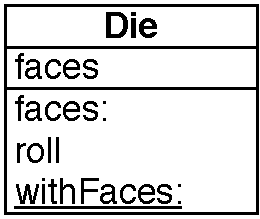
\includegraphics[width=0.25\textwidth]{/Users/ducasse/Workspace/FirstCircle/MyBooks/Bk-Writing/PharoBooks/LearningOOPWithPharoTrans/_result/pdf/Chapters/DSL/figures/OneClassDiceDesign.pdf}\caption{A single class with a couple of messages. Note that the method \textcode{withFaces:} is  a class method.\label{figOneClassDiceDesign}}\end{center}
\end{figure}


\begin{displaycode}{plain}
Object subclass:
	... Your solution ...
\end{displaycode}

In the \textcode{initialization} protocol, define the method \textcode{initialize} so that it simply sets the default number of faces to 6. 

\begin{displaycode}{plain}
Die >> initialize
	... Your solution ...
\end{displaycode}

Do not hesitate to add a class comment. 

Now define a method to return the number of faces an instance of \textcode{Die} has.

\begin{displaycode}{plain}
Die >> faces
	^ faces
\end{displaycode}

Now your tests should all pass (and turn green).
\section{Rolling a die}
To roll a die you should use the method from Number \textcode{atRandom} which draws randomly a 
number between one and the receiver. For example \textcode{10 atRandom} draws number between 1 to 10. 
Therefore we define the method \textcode{roll}:

\begin{displaycode}{plain}
Die >> roll
	... Your solution ...
\end{displaycode}

Now we can create an instance \textcode{Die new} and send it the message  \textcode{roll} and get a result.
Do \textcode{Die new inspect} to get an inspector and then type in the bottom pane \textcode{self roll}.
You should get an inspector like the one shown in Figure \ref{figDiceNoDetail}. With it you can interact with a die by writing expression in the bottom pane.


\begin{figure}

\begin{center}
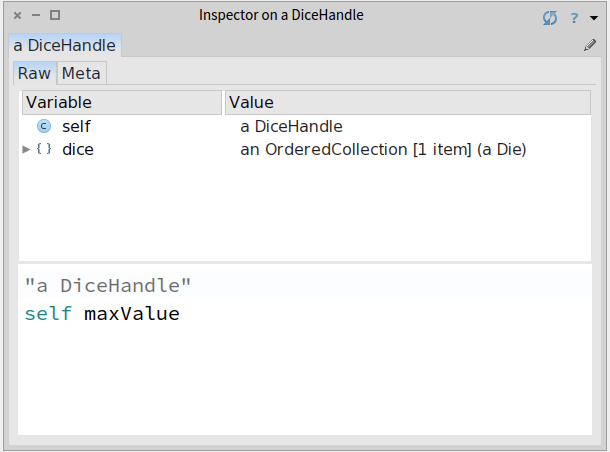
\includegraphics[width=0.6\textwidth]{/Users/ducasse/Workspace/FirstCircle/MyBooks/Bk-Writing/PharoBooks/LearningOOPWithPharoTrans/_result/pdf/Chapters/DSL/figures/DiceNoDetail.png}\caption{Inspecting and interacting with a die.\label{figDiceNoDetail}}\end{center}
\end{figure}


 
\section{Creating another test}
But better, let us define a test that verifies that rolling a new created dice with a default 6 faces only returns 
value comprised between 1 and 6. This is what the following test method is actually specifying.
 

\begin{displaycode}{plain}
DieTest >> testRolling
	| d |
	d := Die new.
	10 timesRepeat: [ self assert: (d roll between: 1 and: 6) ]
\end{displaycode}

\begin{important}
Often it is better to define the test even before the code it tests. Why? Because you can think about the API of your objects and a scenario that illustrate their correct behavior. It helps you to program your solution.
\end{important}
\section{Instance creation interface}
We would like to get a simpler way to create \textcode{Die} instances. For example we want to create a 20-faces die as follows: \textcode{Die withFaces: 20} instead of always have to send the new message to the class as in \textcode{Die new faces: 20}.
Both expressions are creating the same die but one is shorter.

Let us look at it: 

\begin{itemize}
\item In the expression \textcode{Die withFaces:}, the message \textcode{withFaces:} is sent to the class \textcode{Die}. It is not new, we constantly sent the message \textcode{new} to \textcode{Die} to created instances. 
\item Therefore we should define a method that will be executed 
\end{itemize}

Let us define a test for it.

\begin{displaycode}{plain}
DieTest >> testCreationIsOk
	self assert: (Die withFaces: 20) faces equals: 20
\end{displaycode}

What the test clearly shows is that we are sending a message to the \textbf{class} \textcode{Die} itself.
\subsection{Defining a class method}
Define the \textit{class} method \textcode{withFaces:} as follows:

\begin{itemize}
\item Click on the class button in the browser to make sure that you are editing a \textbf{class} method.
\item Define the method as follows: 
\end{itemize}

\begin{displaycode}{plain}
Die class >> withFaces: aNumber
	"Create and initialize a new die with aNumber faces."
	| instance |
	instance := self new.
	instance faces: aNumber.
	^ instance
\end{displaycode}

Let us explain this method

\begin{itemize}
\item The method \textcode{ withFaces:} creates an instance using the message \textcode{new}. Since \textcode{self} represents the receiver of the message and the receiver of the message is the class \textcode{Die} itself then \textcode{self} represents the class \textcode{Die}. 
\item Then the method sends the message \textcode{faces:} to the instance and 
\item Finally returns the newly created instance.
\end{itemize}

Pay really attention that a class method \textcode{withFaces:} is sent to a class, and an instance method sent to the newly created instance \textcode{faces:}. Note that the class method could have also named \textcode{faces:} or any name we want, it does not matter, it is executed when the receiver is the class \textcode{Die}.

This test will not work since we did not create yet the method \textcode{faces:}.  This is now the time to define it. Pay attention the method \textcode{faces:} is sent to an instance of the class \textcode{Die} and not the class itself. It is an instance method, therefore make sure that you deselected the class button before editing it.

\begin{displaycode}{plain}
Die >> faces: aNumber
	faces := aNumber
\end{displaycode}

Now your tests should run. So even if the class \textcode{Die} could implement more behavior, we are ready to implement a die handle. 

\begin{important}
A class method is a method executed in reaction to messages sent to a \textit{class}. It is defined on the class side of the class. In \textcode{Die withFaces: 20}, the message \textcode{withFaces:} is sent to the class \textcode{Die}. In \textcode{Die new faces: 20}, the message \textcode{new} is sent to the \textit{class} \textcode{Die} and the message \textcode{faces:} is sent to the \textit{instance} returned by \textcode{Die new}. 
\end{important}
\subsection{{[}Optional{]} Alternate instance creation definition}
 In a first reading you can skip this section. The \textit{class} method definition \textcode{withFaces:} above is strictly equivalent to the one below.

\begin{displaycode}{plain}
Die class >> withFaces: aNumber
	^ self new faces: aNumber; yourself
\end{displaycode}

Let us explain it a bit. \textcode{self} represents the class \textcode{Die} itself. Sending it the message \textcode{new}, we create an instance and send it the \textcode{faces:} message. And we return the expression. So why do we need the message \textcode{yourself}. The message \textcode{yourself} is needed to make sure that whatever value the instance message \textcode{faces:} returns, the instance creation method we are defining returns the new created instance. You can try to redefine the instance method \textcode{faces:} as follows:

\begin{displaycode}{plain}
Die >> faces: aNumber 
	faces := aNumber. 
	^ 33
\end{displaycode}

Without the use of \textcode{yourself}, \textcode{Die withFaces: 20} will return 33. With \textcode{yourself} it will return the instance.

The trick is that \textcode{yourself} is a simple method defined on \textcode{Object} class: The message \textcode{yourself} returns the receiver of a message.
The use of \textcode{;} sends the message to the receiver of the previous message (here \textcode{faces:}).  The message \textcode{yourself} is then sent to the object resulting from the execution of the expression \textcode{self new} (which returns a new instance of the class \textcode{Die}), as a consequence it returns the new instance. 
\section{First specification of a die handle}
Let us define a new class \textcode{DieHandle} that represents a die handle. 
The following code snippet shows the API that we would like to offer for now (as shown in Figure \ref{fig:DiceDesign}). We create a new handle then add some dice to it. We will use this kind of expressions in future tests below.


\begin{figure}

\begin{center}
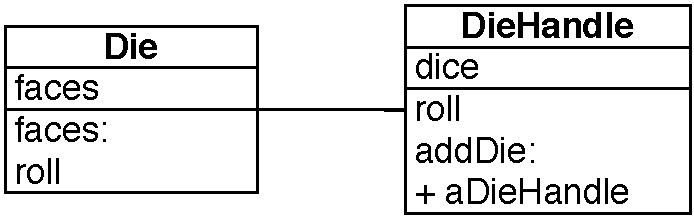
\includegraphics[width=0.6\textwidth]{/Users/ducasse/Workspace/FirstCircle/MyBooks/Bk-Writing/PharoBooks/LearningOOPWithPharoTrans/_result/pdf/Chapters/DSL/figures/DiceDesign.pdf}\caption{A die handle is composed of dice.\label{fig:DiceDesign}}\end{center}
\end{figure}


\begin{displaycode}{plain}
DieHandle new 
	addDie: (Die withFaces: 6);
	addDie: (Die withFaces: 10);
	yourself
\end{displaycode}

Of course we will define tests first for this new class. We define the class \textcode{DieHandleTest}.

\begin{displaycode}{plain}
TestCase subclass: #DieHandleTest
	instanceVariableNames: ''
	classVariableNames: ''
	package: 'Dice'
\end{displaycode}
\subsection{Testing a die handle}
We define a new test method as follows. We create a new handle and add one die of 6 faces and one die of 10 faces.
We verify that the handle is composed of two dice. 

\begin{displaycode}{plain}
DieHandleTest >> testCreationAdding
	| handle |
	handle := DieHandle new 
			addDie: (Die withFaces: 6);
			addDie: (Die withFaces: 10);
			yourself.
	self assert: handle diceNumber = 2.
\end{displaycode}

In fact we can do it better. Let us add a new test method to verify that we can even add
two dice having the same number of faces. 

\begin{displaycode}{plain}
DieHandleTest >> testAddingTwiceTheSameDice
	| handle |
	handle := DieHandle new. 
	handle addDie: (Die withFaces: 6).
	self assert: handle diceNumber = 1.
	handle addDie: (Die withFaces: 6).
	self assert: handle diceNumber = 2.
\end{displaycode}

Now that we specified what we want, we should implement the expected class and messages. 
Easy!
\section{Defining the DieHandle class}
The class \textcode{DieHandle} inherits from \textcode{Object} and it defines one instance variable to hold the dice it contains. 

\begin{displaycode}{plain}
Object subclass: ...
	... Your solution ...
\end{displaycode}

We simply initialize it so that its instance variable \textcode{dice} contains an instance of \textcode{OrderedCollection}.

\begin{displaycode}{plain}
DieHandle >> initialize
	... Your solution ...
\end{displaycode}

Then define a simple method \textcode{addDie:} to add a die to the list of dice of the handle. You can use the message \textcode{add:} sent to a collection.

\begin{displaycode}{plain}
DieHandle >> addDie: aDie 
	... Your solution ...
\end{displaycode}

Now you can execute the code snippet and inspect it. You should get an inspector as shown in Figure \ref{DieHandleNoDetail} 

\begin{displaycode}{plain}
DieHandle new 
	addDie: (Die withFaces: 6);
	addDie: (Die withFaces: 10);
	yourself
\end{displaycode}


\begin{figure}

\begin{center}
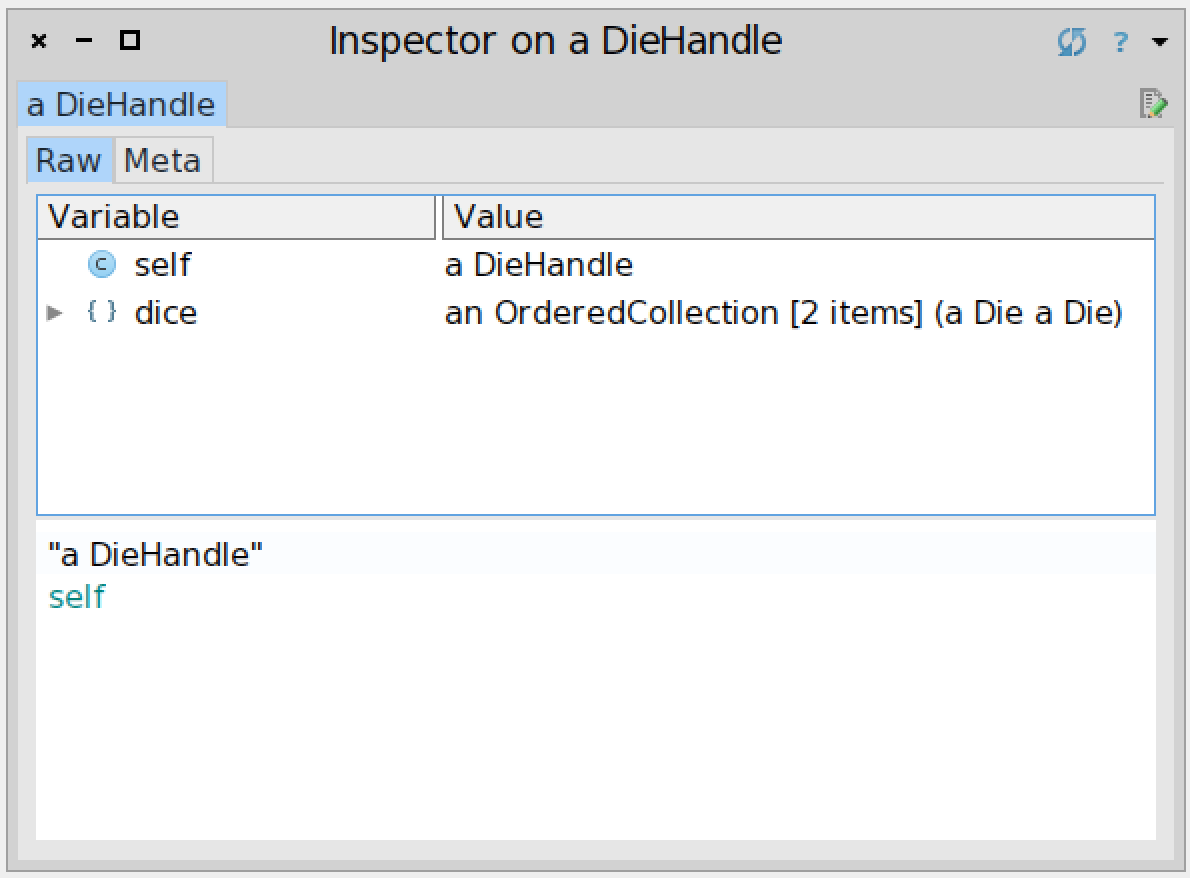
\includegraphics[width=0.6\textwidth]{/Users/ducasse/Workspace/FirstCircle/MyBooks/Bk-Writing/PharoBooks/LearningOOPWithPharoTrans/_result/pdf/Chapters/DSL/figures/DiceHandleNoDetail.png}\caption{Inspecting a DieHandle.\label{DieHandleNoDetail}}\end{center}
\end{figure}


Finally we should add the method \textcode{diceNumber} to the \textcode{DieHandle} class to be able to get the number of dice of the handle. We just return the size of the dice collection.

\begin{displaycode}{plain}
DieHandle >> diceNumber  
	^ dice size
\end{displaycode}

Now your tests should run and this is a good moment to save and publish your code. 
\section{Improving programmer experience}
Now when you open an inspector you cannot see well the dice that compose the die handle. Click on the \textcode{dice} instance variable and you will only get a list of \textcode{a Dice} without further information. What we would like to get is something like \textcode{a Die (6)} or \textcode{a Die (10)} so that in a glance we know the faces a die has. 

\begin{displaycode}{plain}
DieHandle new 
	addDie: (Die withFaces: 6);
	addDie: (Die withFaces: 10);
	yourself
\end{displaycode}

This is the  message \textcode{printOn:} that is responsible to provide a textual representation of the message receiver. By default, it just prints the name of the class prefixed with \textcode{'a'} or \textcode{'an'}. So we will enhance the \textcode{printOn:} method of the \textcode{Die} class to provide more information. Here we simply add the number of faces surrounded by parenthesis. The \textcode{printOn:} message is sent with a stream as argument. This is in such stream that we should add information. We use the message \textcode{nextPutAll:} to add a number of characters to the stream. We concatenate the characters to compose \textcode{()} using the message \textcode{,} comma defined on collections (and that concatenate collections and strings).

\begin{displaycode}{plain}
Die >> printOn: aStream

	super printOn: aStream.
	aStream nextPutAll: ' (', faces printString, ')'
\end{displaycode}

Now in your inspector you can see effectively the number of faces a die handle has as shown by Figure \ref{diceDetail} and it is now easier to check the dice contained inside a handle (See Figure \ref{DieHandleDetail}).


\begin{figure}

\begin{center}
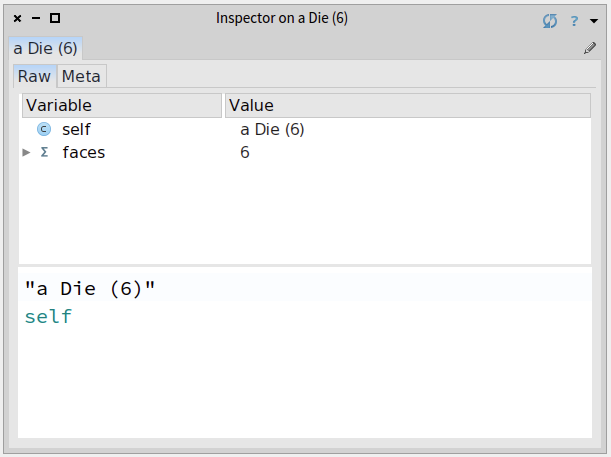
\includegraphics[width=0.7\textwidth]{/Users/ducasse/Workspace/FirstCircle/MyBooks/Bk-Writing/PharoBooks/LearningOOPWithPharoTrans/_result/pdf/Chapters/DSL/figures/DiceDetail.png}\caption{Die details.\label{diceDetail}}\end{center}
\end{figure}
 


\begin{figure}

\begin{center}
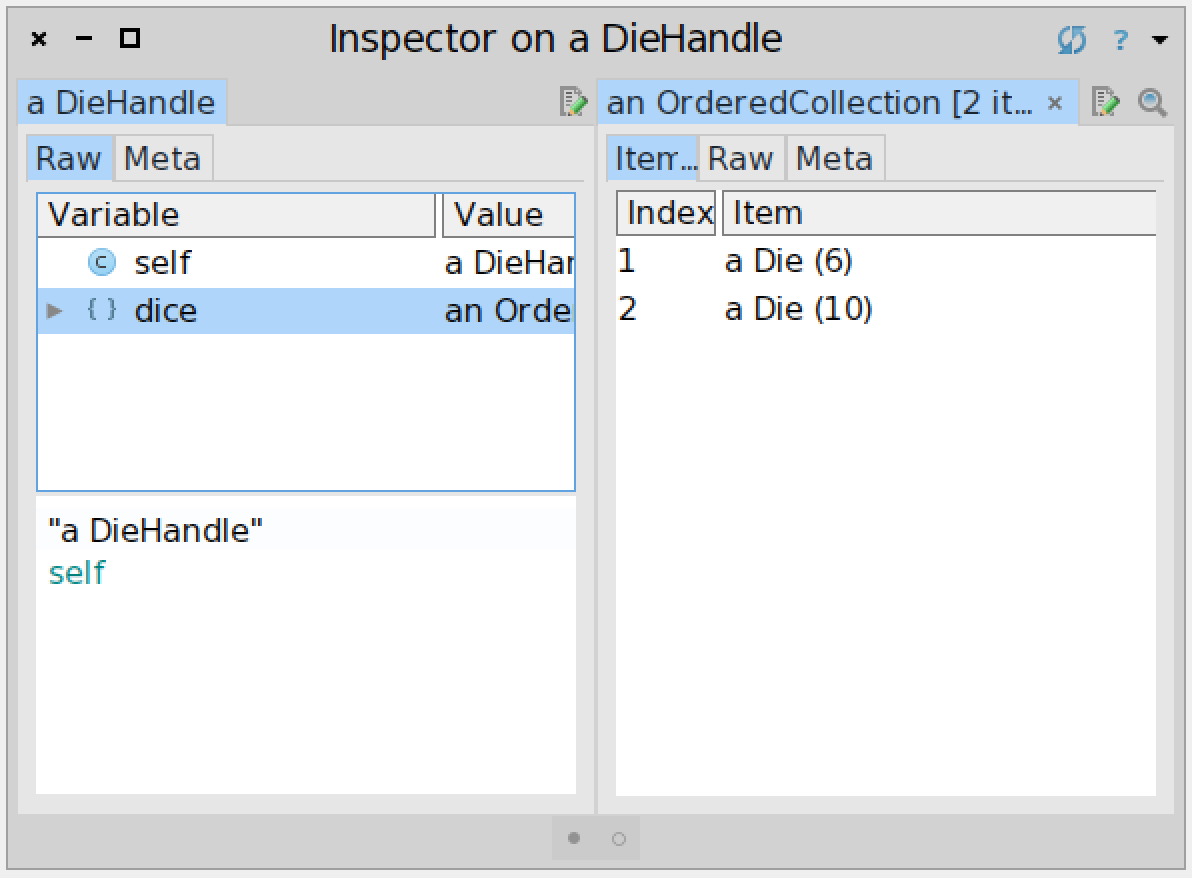
\includegraphics[width=0.9\textwidth]{/Users/ducasse/Workspace/FirstCircle/MyBooks/Bk-Writing/PharoBooks/LearningOOPWithPharoTrans/_result/pdf/Chapters/DSL/figures/DiceHandleDetail.png}\caption{A die handle with more information.\label{DieHandleDetail}}\end{center}
\end{figure}
 

\textbf{Note} This implementation of \textcode{printOn:} is suboptimal. Indeed during the message \textcode{faces printString}, it creates a separate stream instead of using the one pass as argument.
To understand the problem you can have a look at the implementation of the method \textcode{printString} defined in the class \textcode{Object}. 

\begin{displaycode}{plain}
Die >> printOn: aStream
	
	super printOn: aStream.
	aStream 
		nextPutAll: '(';
		print: faces; 
		nextPutAll: ')'
\end{displaycode}
\section{Rolling a die handle}
Now we can define the rolling of a die handle by simply summing result of rolling each of its dice. 
Implement the \textcode{roll} method of the \textcode{DieHandle} class. This method must collect the results of rolling each dice of the handle and sum them.

You may want to have a look at the method \textcode{sum:} in the class \textcode{Collection} or use a simple loop such as \textcode{do:} to iterate over the dice.

\begin{displaycode}{plain}
DieHandle >> roll
	... Your solution ...
\end{displaycode}

Now we can send the message \textcode{roll} to a die handle.

\begin{displaycode}{plain}
handle := DieHandle new 
		addDie: (Die withFaces: 6);
		addDie: (Die withFaces: 10);
		yourself.
handle roll
\end{displaycode}

Define a test to cover such behavior. Rolling an handle of n dice should be between n and the sum of the face number of each die. 

\begin{displaycode}{plain}
DieHandleTest >> testRoll
	... Your solution ...
\end{displaycode}
\section{About Dice and DieHandle API}
It is worth to spend some times looking at the relationship between \textcode{DieHandle} and \textcode{Dice}. 
A die handle is composed of dices. What is an important design decision is that the API of the main behavior (\textcode{roll}) is the same for a die or a die handle. You can send the message \textcode{roll} to a dice or a die handle. This is an important property.

Why? Because it means that from a client perspective, she/he can treat the receiver without having to take care about the kind of object it is manipulating. A client just sends the message \textcode{roll} to an object and get back a number (as shown in Figure \ref{figDieHandleComposition}). The client is not concerned by the fact that the receiver is composed out a simple object or a complex one. Such design decision supports the \textit{Don't ask, tell} principle.


\begin{figure}

\begin{center}
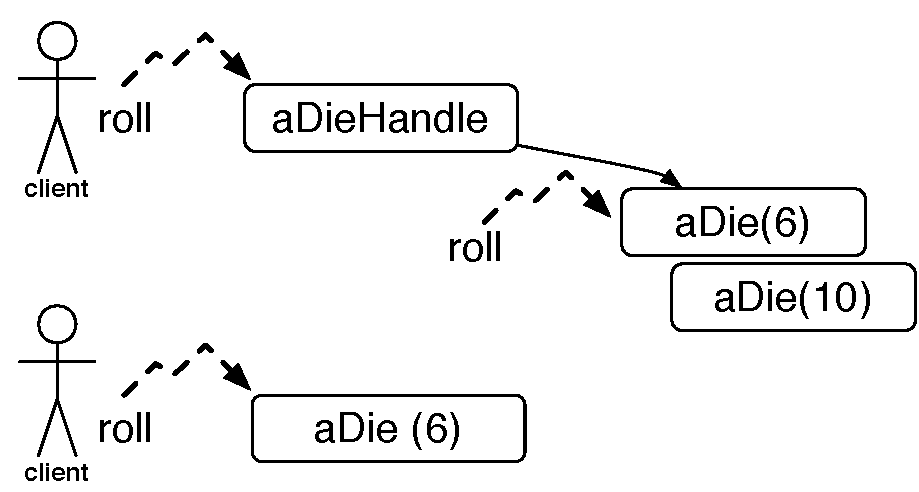
\includegraphics[width=0.6\textwidth]{/Users/ducasse/Workspace/FirstCircle/MyBooks/Bk-Writing/PharoBooks/LearningOOPWithPharoTrans/_result/pdf/Chapters/DSL/figures/DiceHandleComposition.pdf}\caption{A polymorphic API supports the \textit{Don't ask, tell} principle.\label{figDieHandleComposition}}\end{center}
\end{figure}


\begin{important}
Offering polymorphic API is a tenet of good object-oriented design. It enforces the \textit{Don't ask, tell} principle. Clients do not have to worry about the type of the objects to whom they talk to. 
\end{important}

For example we can write the following expression that adds a die and a dieHandle to a collection and collect the different values (we convert the result into an array so that we can print it in the book).

\begin{displaycode}{plain}
| col |
col := OrderedCollection new. 
col add: (Die withFaces: 20).
col add: (DieHandle new addDie: (Die withFaces: 4); yourself).
(col collect: [:each | each roll]) asArray
>>> #(17 3) 
\end{displaycode}
\subsection{About composition}
Composite objects such document objects (a book is composed of chapters, a chapter is composed of sections, a section is composed of paragraphs) have often a more complex composition relationship than the composition between die and die handle. Often the composition is recursive in the sense that an element can be the whole: for example, a diagram can be composed of lines, circles, and other diagrams. We will see an example of such composition in the Expression Chapter \ref{cha:expressions}.
\section{Role playing syntax}
Now we are ready to offer a syntax following practice of role playing game, i.e., using \textcode{2 D20} to create a handle of two dice with 20 faces each.  For this purpose we will define class extensions: we will define methods in the class \textcode{Integer} but these methods will be only available when the package Dice will be loaded. 

But first let us specify  what we would like to obtain by writing a new  test in the class \textcode{DieHandleTest}. Remember
to always take  any opportunity to write tests.  When we execute \textcode{2 D20} we  should get a new handle  composed of two
dice and can verify that. This is what the method \textcode{testSimpleHandle} is doing.

\begin{displaycode}{plain}
DieHandleTest >> testSimpleHandle
	self assert: 2 D20 diceNumber = 2.
\end{displaycode}

Verify that the test is not working! It is much more satisfactory to get a test running when it was not working before. Now define the method \textcode{D20} with a protocol named \textcode{*NameOfYourPackage} (\textcode{'*Dice}' if you named your package \textcode{'Dice'}).
The \textcode{*} (star) prefixing a protocol name indicates that the protocol and its methods belong to another package than the package of the class. Here we want to say that while the method \textcode{D20} is defined in the class \textcode{Integer}, it should be saved with the package \textcode{Dice}. 
 
The method \textcode{D20} simply creates a new die handle, adds the correct number of dice to this handle, and returns the handle.

\begin{displaycode}{plain}
Integer >> D20
	... Your solution ...
\end{displaycode}
\subsection{About class extensions}
We asked you to place the method \textcode{D20} in a protocol starting with a star and having the name of the package (\textcode{'*Dice'}) because we want this method to be saved (and packaged) together with the code of the classes we already created (\textcode{Die}, \textcode{DieHandle},...) 
Indeed in Pharo we can define methods in classes that are not defined in our package. Pharoers call this action a class extension: we can add methods to a class that is not ours. For example \textcode{D20} is defined on the class \textcode{Integer}. Now such methods only make sense when the package \textcode{Dice} is loaded. 
This is why we want to save and load such methods with the package we created. This is why we are defining the protocol as \textcode{'*Dice'}.
This notation is a way for the system to know that it should save the methods with the package and not with the package of the class \textcode{Integer}. 

Now your tests should pass and this is probably a good moment to save your work either by publishing your package and to save your image. 

We can do the same for the default dice with different faces number: 4, 6, 10, and 20. But we should avoid duplicating logic and code. So first we will introduce a new method \textcode{D:} and based on it we will define all the others.

Make sure that all the new methods are placed in the protocol \textcode{'*Dice'}. To verify you can press the button Browse of the Monticello package browser and you should see the methods defined in the class \textcode{Integer}. 

\begin{displaycode}{plain}
Integer >> D: anInteger
	... Your solution ...
\end{displaycode}

\begin{displaycode}{plain}
Integer >> D4
	^ self D: 4
\end{displaycode}

\begin{displaycode}{plain}
Integer >> D6
	^ self D: 6
\end{displaycode}

\begin{displaycode}{plain}
Integer >> D10
	^ self D: 10
\end{displaycode}

\begin{displaycode}{plain}
Integer >> D20
	^ self D: 20
\end{displaycode}

We have now a compact form to create dice and we are ready for the last part: the addition of handles. 
\section{Handle's addition}
Now what is missing is that possibility to add several handles as follows: \textcode{2 D20 + 3 D10}. Of course let's write a test first to be clear on what we mean.

\begin{displaycode}{plain}
DieHandleTest >> testSumming
	| handle |
	handle := 2 D20 + 3 D10.
	self assert: handle diceNumber = 5.
\end{displaycode}

We will define a method \textcode{+} on the \textcode{DieHandle} class. In other languages this is often not possible or is based on operator overloading. In Pharo \textcode{+} is just a message as any other, therefore we can define it on the classes we want.

Now we should ask ourself what is the semantics of adding two handles. Should we modify the receiver of the expression or create a new one. We preferred a more functional style and choose to create a third one. 

The method \textcode{+} creates a new handle then add to it the dice of the receiver and the one of the handle passed as argument to the message. Finally we return it. 

\begin{displaycode}{plain}
DieHandle >> + aDieHandle
	... Your solution ... 
\end{displaycode}

Now we can execute the method \textcode{(2 D20 + 1 D6) roll} nicely and start playing role playing games, of course.
\section{Conclusion}
This chapter illustrates how to create a small DSL based on the definition of some domain classes (here \textcode{Dice} and  
 \textcode{DieHandle}) and the extension of core class such as \textcode{Integer}. It also shows that we can create packages with all the methods that are needed even when such methods are defined on classes external (here \textcode{Integer}) to the package.  
It shows that in Pharo we can use usual operators such as \textcode{+} to express natural models.
\part{Sending messages}\chapter{Sending a message is making a choice}\label{cha:messages}
In this chapter we explore an \textit{essential} point of object-oriented programming: Sending a message is making a choice! 

Object-oriented programming books often present \textit{late binding}: the fact that the method to execute will only be determined at runtime based on the receiver. In fact sending a message uses late binding to select the correct method. I like to use the term \textit{sending a message} because it stresses that simple
actions, such as sending a message, are also a powerful feature when used well. 

This aspect is often not really well put in perspective in teaching materials. Lectures often focus on inheritance but understanding the power of message passing it crucial to build good design.
This point is so central for me that this is the first point that I explain when I start lectures on advanced design to people already understanding object-oriented programming. In addition, most of
the Design Patterns are based on the fact that sending a message is actually selecting the correct method
based on the message receiver.

To illustrate how sending a message performs a dynamic choice, I will start taking a simple example available in the core of Pharo: the Booleans. Pharo defines Booleans as two objects: \textcode{true} and \textcode{false}. They are so fundamental that you cannot change their value. 
Still their implementation also use late binding in a really elegant way. 
 I will explain how the Boolean negation and the disjunction (or) are implemented. Then I will step back and analyse the forces in presence and their importance. 
\section{Negation: the not message}
Boolean negation has nothing special in Pharo: negating a boolean returned the negated value! 
For example the snippets below show this conventional behavior and vice versa.

Sending the message \textcode{not} to the Boolean \textcode{true} returns the Boolean \textcode{false}. 

\begin{displaycode}{plain}
true not
>>> false
\end{displaycode}

\begin{displaycode}{plain}
false not
>>> true
\end{displaycode}

Nothing fancy. Of course the message \textcode{not} can be sent to Boolean expressions (i.e. expressions whose execution return Booleans) as shown below:

\begin{displaycode}{plain}
(2 * 4 > 3) not
>>> false
\end{displaycode}

\begin{displaycode}{plain}
(#(1 2 3) includes: 5) not
>>> true
\end{displaycode}

Now while Pharo follows traditional Boolean logic, what is less traditional is the implementation of the way the computation is done to answer the correct value.
\section{Implementing not}
Take a couple of minutes and a piece of paper and think about the way you would implement this message. Try really to write the code for real.
\subsection{A first hint. }
A first hint that I can give you is that the solution (used in Pharo and that we want to study) does not use explicit conditional such as \textcode{ifTrue:} or \textcode{ifTrue:ifFalse:}.

Take a bit more time to think how you can implement not. 
What we can tell you is the solution is not based on bit fiddling and logical operation on small integers. The solution we are looking for is simple and elegant.
\subsection{A second hint.}
The second hint is that \textcode{true} and \textcode{false} are instances of different classes. \textcode{true} is (the unique) instance of the class \textcode{True} while \textcode{false} is (the unique) instance of the class \textcode{False}. Note the uppercase on class names. This situation is depicted in Figure \ref{figTrueFalseOnly}.

What you should see is that the fact that the solution has two different classes opens the door to have two different \textcode{not} implementations as shown by Figure \ref{figTrueFalseOnlySelectors}. Indeed, as we mention in early chapters, we can have one message and multiple methods that we will be selected and executed depending on the receiver of the message. 

Now you should be ready to get the solution. We should have a definition for the \textcode{true} defined in the class \textcode{True} and one for \textcode{false} in the class \textcode{False}.


\begin{figure}

\begin{center}
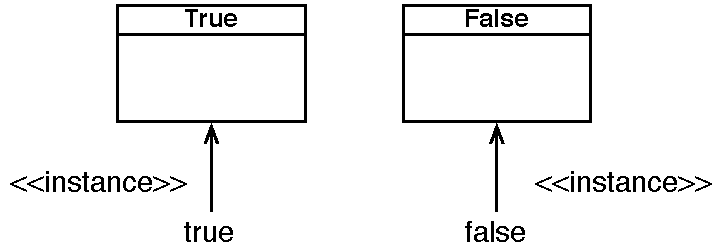
\includegraphics[width=0.55\textwidth]{/Users/ducasse/Workspace/FirstCircle/MyBooks/Bk-Writing/PharoBooks/LearningOOPWithPharoTrans/_result/pdf/Chapters/MessageSending/figures/BooleanTrueAndFalseSolelyWithInstances.pdf}\caption{The two classes \textcode{True} and \textcode{False} and their respective unique instances \textcode{true} and \textcode{false}.\label{figTrueFalseOnly}}\end{center}
\end{figure}



\begin{figure}

\begin{center}
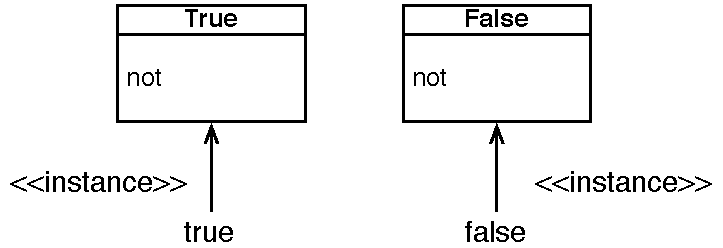
\includegraphics[width=0.65\textwidth]{/Users/ducasse/Workspace/FirstCircle/MyBooks/Bk-Writing/PharoBooks/LearningOOPWithPharoTrans/_result/pdf/Chapters/MessageSending/figures/BooleanTrueAndFalseWithNotMethodSelectors.pdf}\caption{Two methods for one message.\label{figTrueFalseOnlySelectors}}\end{center}
\end{figure}

\subsection{Studying the implementation}

\begin{figure}

\begin{center}
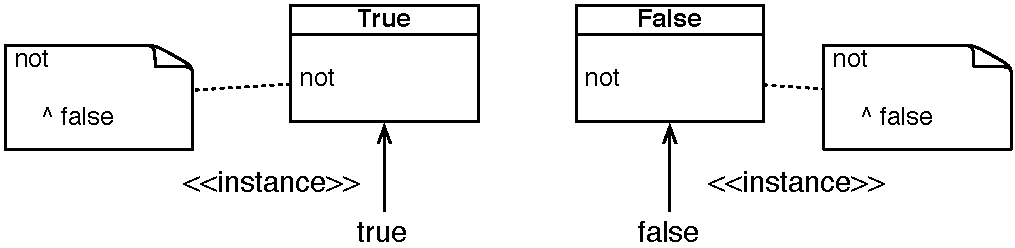
\includegraphics[width=0.75\textwidth]{/Users/ducasse/Workspace/FirstCircle/MyBooks/Bk-Writing/PharoBooks/LearningOOPWithPharoTrans/_result/pdf/Chapters/MessageSending/figures/BooleanTrueAndFalseWithNotMethods.pdf}\caption{Two methods for one message each one returning the other instance.\label{figTrueFalseSolution}}\end{center}
\end{figure}


The implementation of negation (message \textcode{not}) is defined as illustrated in Figure \ref{figTrueFalseSolution} and is shown below. The method \textcode{not} of the class \textcode{True} simply returns the Boolean \textcode{false}. 

\begin{displaycode}{plain}
True >> not
   "Negation--answer false since the receiver is true."
   ^ false
\end{displaycode}

\begin{displaycode}{plain}
False >> not
   "Negation--answer true since the receiver is false."
   ^ true
\end{displaycode}

Figure \ref{figTrueFalseSolutionLookup} shows that sending a message to one of the two Booleans selects the method in the corresponding class. What is important to see is that when a method is executed the receiver is from the class (or subclass we will see that later) that defines the method. We can also say that when we define a method in a given class we know that the receiver is from this class. Obvious, isn't it! But important. The implementation can then use this information as an execution context. This is exactly what the \textcode{not} implementation does. The method \textcode{not} defined on the class \textcode{True} knows that the receiver is true so it just has to return \textcode{false}. 


\begin{figure}

\begin{center}
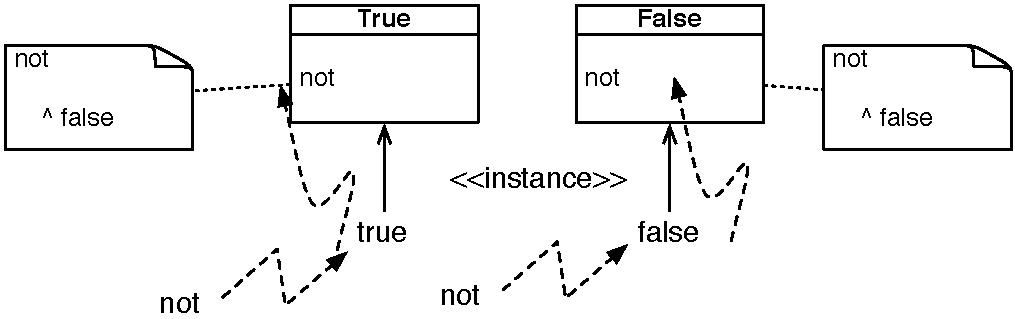
\includegraphics[width=0.75\textwidth]{/Users/ducasse/Workspace/FirstCircle/MyBooks/Bk-Writing/PharoBooks/LearningOOPWithPharoTrans/_result/pdf/Chapters/MessageSending/figures/BooleanTrueAndFalseWithNotMethodsLookup.pdf}\caption{Sending a message selects the method in the class of the receiver.\label{figTrueFalseSolutionLookup}}\end{center}
\end{figure}


\begin{note}
When we define a method in a given class we know that the receiver is from this class. Obvious but important. The implementation can then use this information.
\end{note}

Now we will see if you get it... Let us try with a slightly more complex example.
\section{Implementing disjunction}
Disjunction is also a core functionality of any programming language. In Pharo disjunction is expressed via the message \textcode{\textbar{}}. 
 Here are the traditional tables describing disjunction but expressed in Pharo: first starting with \textcode{true} as receiver.

\begin{tabular}{llll}
\toprule
\textbf{or} & true & false &  \\
true & true & true &  \\
false & true & false &  \\
\bottomrule
\end{tabular}

Here are a couple of examples expressed in Pharo. 

\begin{displaycode}{plain}
true | true
>>> true
\end{displaycode}

\begin{displaycode}{plain}
true | false 
>>> true
\end{displaycode}

\begin{displaycode}{plain}
false | false 
>>> false
\end{displaycode}

For the record, in fact the message \textcode{\textbar{}} implements an eager disjunction since it asks the value of its argument even when not needed and Pharo also offers lazy disjunction implemented in the message \textcode{or:} which only requests the argument value if needed.
\subsection{When receiver is true.}
Propose an implementation of the disjunction for the first case: i.e. when the receiver is the object \textcode{true}.

\begin{tabular}{llll}
\toprule
\textbf{or} & true & false &  \\
true & true & true &  \\
\bottomrule
\end{tabular}

 What you should have learned from the implementation of \textcode{not} is that you have two different methods taking advantage of the fact that they know what is the receiver during their execution. 

\begin{displaycode}{plain}
true | true 
>>> true
\end{displaycode}

\begin{displaycode}{plain}
true | false 
>>> true
\end{displaycode}

\begin{displaycode}{plain}
true | anything 
>>> true
\end{displaycode}

When you look at the table we see that when the receiver is \textcode{true} the result is the same as the receiver (i.e. \textcode{true}). In Pharo the method \textcode{\textbar{}} on class \textcode{True} express this as follows: 

\begin{displaycode}{plain}
True >> | aBoolean
   "Evaluating Or -- answer true since the receiver is true."
   ^ true
\end{displaycode}
\subsection{When receiver is false.}
Similarly let us study the Boolean table relative to false as receiver. 

\begin{tabular}{llll}
\toprule
\textbf{or} & true & false &  \\
false & true & false &  \\
\bottomrule
\end{tabular}

Here are some snippets

\begin{displaycode}{plain}
false | true 
>>> true
\end{displaycode}

\begin{displaycode}{plain}
false | false 
>>> false
\end{displaycode}

\begin{displaycode}{plain}
false | anything 
>>> anything
\end{displaycode}

We see that when the receiver is \textcode{false}, the result of the disjunction is the other argument. In Pharo the method \textcode{\textbar{}} on class \textcode{False} is then as follows: 

\begin{displaycode}{plain}
False >> | aBoolean
   "Evaluating Or -- answer with the argument, aBoolean."
   ^ aBoolean
\end{displaycode}


\begin{figure}

\begin{center}
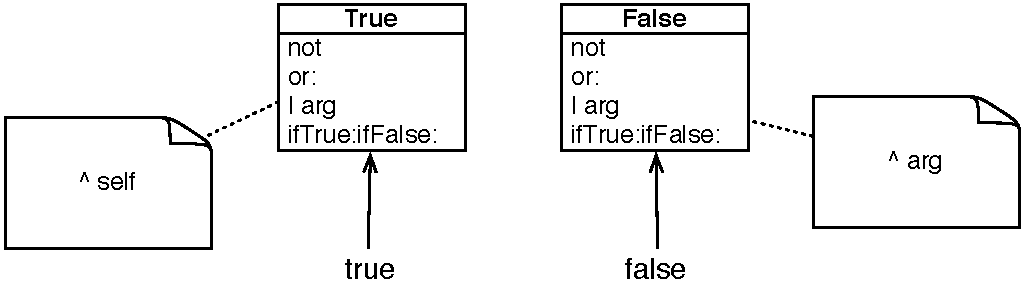
\includegraphics[width=0.8\textwidth]{/Users/ducasse/Workspace/FirstCircle/MyBooks/Bk-Writing/PharoBooks/LearningOOPWithPharoTrans/_result/pdf/Chapters/MessageSending/figures/BooleanNoHiearchyAndInstancesWithOrMethods.pdf}\caption{Disjunction implementation: two methods.\label{/Users/ducasse/Workspace/FirstCircle/MyBooks/Bk-Writing/PharoBooks/LearningOOPWithPharoTrans/_result/pdf/Chapters/MessageSending/figures/BooleanNoHiearchyAndInstancesWithOrMethods.pdf}}\end{center}
\end{figure}

\section{About ifTrue:ifFalse: implementation}
Now you should start to get the principle. Let us see how it works to also express conditional messages such as \textcode{ifTrue:ifFalse:}. Yes fundamental messages such as conditionals can be expressed using the same mechanism: late binding.

What you see with the following snippet is that message \textcode{ifTrue:ifFalse:} is expecting two different blocks as argument. 

\begin{displaycode}{plain}
4 factorial > 20
	ifTrue: [ 'bigger' ]
	ifFalse: [ 'smaller' ]
>>> 'bigger'
\end{displaycode}

Now you should know that to execute a block you should use the message \textcode{value} as illustrated:

\begin{displaycode}{plain}
[1 + 3] value
>>> 4
\end{displaycode}

Block can contain any expressions. The execution of the following block will open the Pharo logo.

\begin{displaycode}{plain}
[ (ZnEasy getPng: 'http://pharo.org/web/files/pharo.png')
       asMorph openInWindow ] value
\end{displaycode}

Let us come back to the case of condition and in particular to the message \textcode{ifTrue:ifFalse:}.
Based on the receiver we should execute the corresponding block from the \textcode{ifTrue:ifFalse:} method. When the expression (\textcode{4 factorial \textgreater{} 20} in the example above) is true we should execute the \textcode{ifTrue:} argument, when it is false we should execute the \textcode{ifFalse:} argument. 
\subsection{Implementation. }
The implementations is then simple and elegant.  In the \textcode{True} class, we want to execute the corresponding block, 
the one passed as \textcode{ifTrue:} argument as shown in Figure \ref{figFT}. 

\begin{displaycode}{plain}
True >> ifTrue: trueAlternativeBlock ifFalse: falseAlternativeBlock
   ^ trueAlternativeBlock value
\end{displaycode}

Similarly in the \textcode{False} class, we want to execute the corresponding block, 
the one passed as \textcode{ifFalse:} argument. 

\begin{displaycode}{plain}
False >> ifTrue: trueAlternativeBlock ifFalse: falseAlternativeBlock
   ^ falseAlternativeBlock value
\end{displaycode}


\begin{figure}

\begin{center}
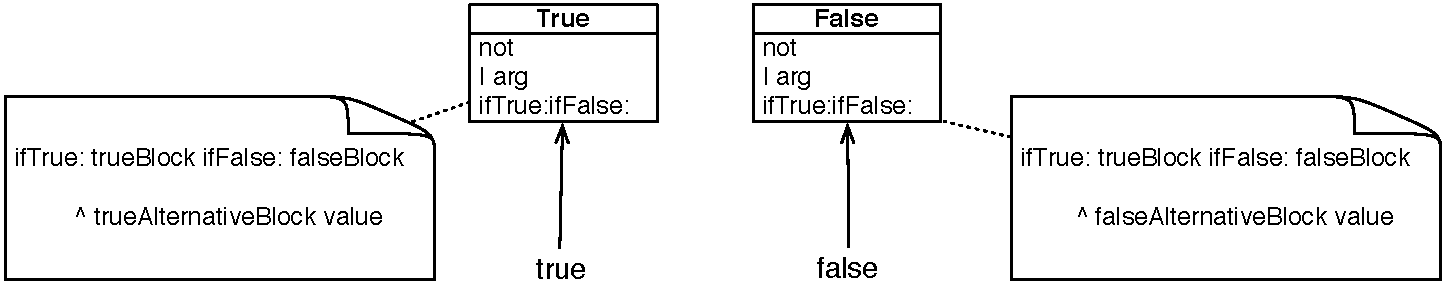
\includegraphics[width=1.0\textwidth]{/Users/ducasse/Workspace/FirstCircle/MyBooks/Bk-Writing/PharoBooks/LearningOOPWithPharoTrans/_result/pdf/Chapters/MessageSending/figures/BooleanNoHiearchyIFTMethods.pdf}\caption{Conditional implementation: again two methods and no explicit tests.\label{figFT}}\end{center}
\end{figure}

\subsection{Optimisation. }
What we show above works! But if you modify it, the modification will not be taken into account. 
This is because in Pharo \textcode{ifTrue:ifFalse:} is used so often and its semantics should not change that the compiler in fact does not send a message but convert it in low-level logic for the virtual machine. 
Now you can invent your own conditional message \textcode{siVrai:siFaux:} for a french version for example and you will see that this implementation works.
\section{What is the point?}
Some readers may be intrigued and think that this is spurious because they will never have to reimplement Booleans in their life. This is true even if there are different versions of Boolean logic such as the ternary logic that contains also unknown value. 

We picked the Boolean examples to illustrate an important point: sending a message is making a choice. The runtime system will dynamically select the method depending on the receiver. This is what is called late binding or dynamic dispatch. Only at execution the correct method is selected. Now the Boolean example is the simplest one I could find to illustrate this point. 
It is also ground breaking in the sense that it touches something as fundamental as Boolean main operations. 

Now the choices can be made over several dozens of classes. For example in Pillar the document processing system in which this book is written there are around 59 different classes expressing different parts of a document: section, title, bold, paragraph... and the same principle applies there. The system selects the correct methods to render text, LaTeX or HTML using exactly the same principle. 

Now most of the time you can express the same using conditions (except for the Boolean example and this is why I asked you to implement Boolean logic since you do not want to have Boolean logic to be based on condition because this is inefficient) as follows:

\begin{displaycode}{plain}
emitHTML: stream
	self == PRList
		ifTrue: [ ... ]
		self == PRParagraph 
			ifTrue: [ ... ]
			...
\end{displaycode}

The problems with such explicit conditions is the following: 

\begin{itemize}
\item First, they are cumbersome to write. Even using case statements as in other languages, the logic can become complex. Imagine for 59 cases of Pillar. Here is a small part of the document hierarchy. 
\end{itemize}

\begin{displaycode}{plain}
PRObject #(''properties'')
        PRDocumentItem #(''counter'')
                PRDocumentGroup #(''children'')
                        PRDocument #()
                        PRHeader #(''level'')
                        PRList #()
                                PROrderedList #()
                                PRUnorderedList #()
                        PRParagraph #()
                        PRReference #(''reference'' ''parameters'')
                                PRFigure #()
                        PRSlide #(''title'' ''label'')
                PRText #(''text'')'
\end{displaycode}

\begin{itemize}
\item Second, such definitions are not modular. It means that adding a new case requires to edit the method and recompile it. While with the dynamic dispatch, we can just add a new class as shown in Figure \ref{figFat}. Furthermore this class can just take advantage of an existing one and extend it (as we will explained in Chapter \ref{cha:inheritance}).
\end{itemize}


\begin{figure}

\begin{center}
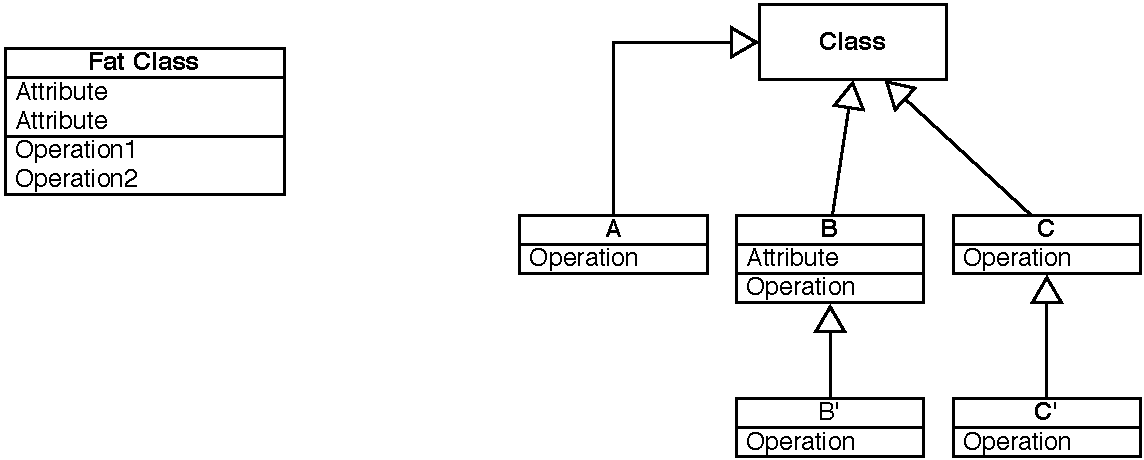
\includegraphics[width=0.8\textwidth]{/Users/ducasse/Workspace/FirstCircle/MyBooks/Bk-Writing/PharoBooks/LearningOOPWithPharoTrans/_result/pdf/Chapters/MessageSending/figures/Design-FatVsDispatch.pdf}\caption{One single class vs. a nice hierarchy.\label{figFat}}\end{center}
\end{figure}


You could think that this is a not a problem but imagine that now for a business you want to ship different products or solutions to your clients. With dynamic dispatch you can simply package alternate code in separate packages and load them independently as shown in Figure \ref{inhNoFatPackage}.


\begin{figure}

\begin{center}
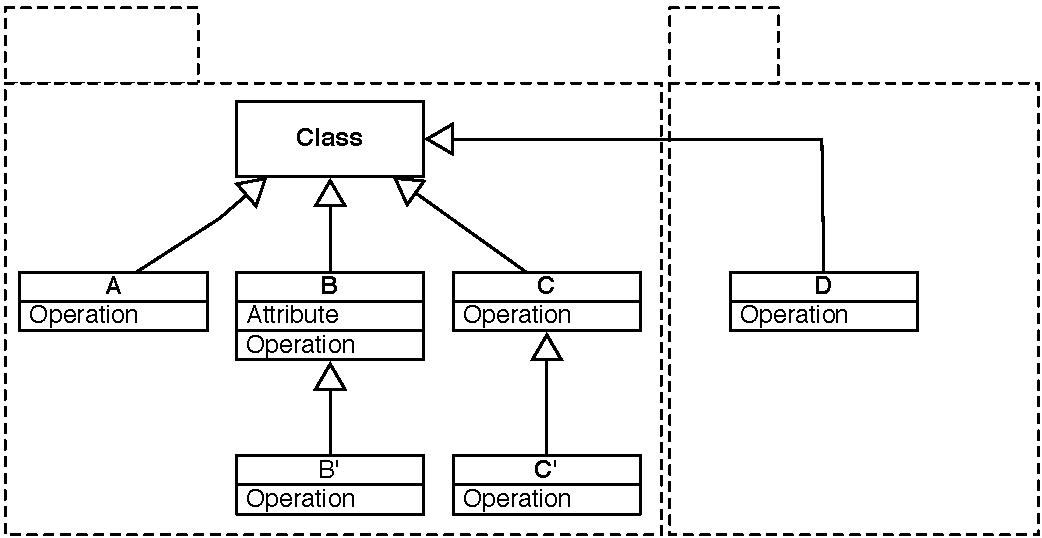
\includegraphics[width=0.8\textwidth]{/Users/ducasse/Workspace/FirstCircle/MyBooks/Bk-Writing/PharoBooks/LearningOOPWithPharoTrans/_result/pdf/Chapters/MessageSending/figures/Design-FatVsDispatchWithPackages.pdf}\caption{One single class vs. a nice hierarchy.\label{inhNoFatPackage}}\end{center}
\end{figure}

\subsection{Classes represent choices}
Sending a message is making a choice. Now the following question is which elements represent choices. Because you can have the possibility to choose something, but if there is only one choice you will not go that far and take advantage of the power of late binding.

In fact, classes represent choices. In the \textcode{Boolean} case you have two choices: one for true, and one for false.
There is a really difference for example between the fat class design (left in Figure \ref{figFat}) and the modular design (right in Figure \ref{figFat}) because we see all the choices which can be made at runtime in the latter case.

When I do code review, I look at how domain variations are represented and if there are enough classes.
What is important to realise is that classes are cheap. It is better to write five little classes than a single huge one.
Some (even smart) people get confused by measuring complexity of a system using number of classes. Having many classes 
representing good abstractions with a single responsibility is much better than having a single class exhibiting multiple responsibilities.
\section{Conclusion}
Sending a message is really powerful since it selects the adequate method to be executed on the receiver. Now this is even more powerful than that: Remember that when we execute a method, one key information we have at hand is that the receiver is an instance from this class (or one of its subclasses as we will see later) and we can take advantage of this information to eliminate tests. Indeed an object executes a method that have been designed to be executed on it. So no need to test more.

Now you should start to understand why in Pharo we are picky about the vocabulary: we use sending a message and not calling a method as in other language. Because sending a message conveys much better the idea that the correct method will be selected and that we do not know a priori which one will be executed. 

In future chapters we will show that sending a message is creating in fact a hook so that other methods can be executed in place. 
\part{Looking at inheritance}
\chapter{Inheritance: Incremental definition and behavior reuse}\label{cha:inheritance}
In Chapter \ref{cha:objectclass}, we presented objects and classes. Objects are entities that communicate exclusively by sending and receiving messages. Objects are described by classes that are factories of objects. Classes define behavior and structure of all their instances: All the instances of a class share the same behavior but have their own private state. 

In this chapter we present the fundamental concept of  \textit{inheritance} that allows a class to reuse and extend the behavior of another class. The idea is that as a programmer we do not want to rewrite from scratch a functionality if another class already offers it. A program specialises the implemented behavior into the new behavior he wants. Inheritance lets us express this concept specialisation.  Using inheritance we create trees of concepts where more precise ones refine more abstract and generic ones. 

Inheritance is based on dynamic method lookup: a method is looked up dynamically within the inheritance tree starting from the class of the receiver. Once this explained we will show that it is possible to get code of a subclass invoked in place of the one of a superclass. 

To illustrate the important points of inheritance, we revisit the example of Chapter \ref{cha:objectclass}. 
\section{Inheritance}
Object-oriented programming is also based on the \textit{incremental} definition of abstractions. This \textit{incremental} definition mechanism is central to support reuse and extension of abstraction. It is called \textit{inheritance}. The idea is that you can define a new abstraction (a class) by refining an existing one (its superclass). We said that a subclass inherits from a superclass. This way we reuse the code of the superclass instead of rewriting everything from scratch.

Class inheritance creates trees of classes. Such trees are based on \textit{generalisation}: a superclass is more generic than its subclasses. A class in such trees can have instances. All the instances share the behavior defined in their class and superclasses.
This is within such trees that the system looks up the method corresponding to a message sent to an instance of a class.

Inheritance supports code reuse because instance variable and methods defined in a root concept (class) are applicable to its refinements (subclasses).


\begin{figure}

\begin{center}
\includegraphics[width=0.6\textwidth]{/Users/ducasse/Workspace/FirstCircle/MyBooks/Bk-Writing/PharoBooks/LearningOOPWithPharoTrans/_result/pdf/Chapters/Inheritance/figures/FileDirectoryV1.pdf}\caption{Two classes understanding similar sets of messages and structuring their instances in a similar way.\label{FileDirectoryV1}}\end{center}
\end{figure}


We will use and extend the simple and naive example of files and directories (seen in Chapter \ref{cha:objectclass}) to illustrate the key aspects of inheritance. While simple, it is enough to show the key properties of inheritance that we want to illustrate: 

\begin{itemize}
\item \textit{incremental definition}: a subclass is defined by expressing the difference to its superclass. A subclass specialises its superclass behavior.
\item \textit{state reuse}: instances of a subclass have at least the state structure of the superclass.
\item \textit{behavior reuse}: upon message reception instances,  when the class of the receiver does not define a method, methods of the superclasses are executed instead.
\item \textit{behavior redefinition (overriding)}: a subclass may change locally a method definition inherited from its superclass.
\item \textit{behavior extension}: a subclass often extends the behavior of one of its superclasses by defining new methods and state.
\item \textit{subclass behavior can be invoked instead of superclass behavior}: behavior defined in a subclass may be executed in place of the one of a superclass. It means that with behavior overriding subclass behavior can be invoked in place of superclass behavior. This is a really important feature of inheritance.
\end{itemize}
\section{Improving files/directories example design}
Let us go back to the example of files and directories introduced in previous chapter. 
When we look at the situation depicted by Figure \ref{FileDirectoryV1} we see that a file is not the same as a directory, even though they share some common state: both have a name and a parent. In addition, they understand some common messages such as \textcode{size}, \textcode{search:}, \textcode{parent:} and \textcode{name:}. Remember that \textcode{size} and \textcode{search:} were not implemented the same way but the messages have indeed the same name. 

Load the code so that you can get the tests that we asked you to define at the end of chapter \ref{cha:objectclass}.

\begin{displaycode}{plain}
Gofer new
	smalltalkhubUser: 'StephaneDucasse' project: 'Loop'; 
	version: 'MyFS2-StephaneDucasse.4';
	load
\end{displaycode}

Verify that the tests are all passing (green).
\subsection{Objectives}
In the following sections we will take advantage of defining a common superclass and reuse its definition as shown in Figure \ref{FileDirectoryWithInheritanceObjective}: It means sharing the maximum structure and behavior between the two classes. We will proceed step by step so that you can see all the steps and understand why this is working.


\begin{figure}

\begin{center}
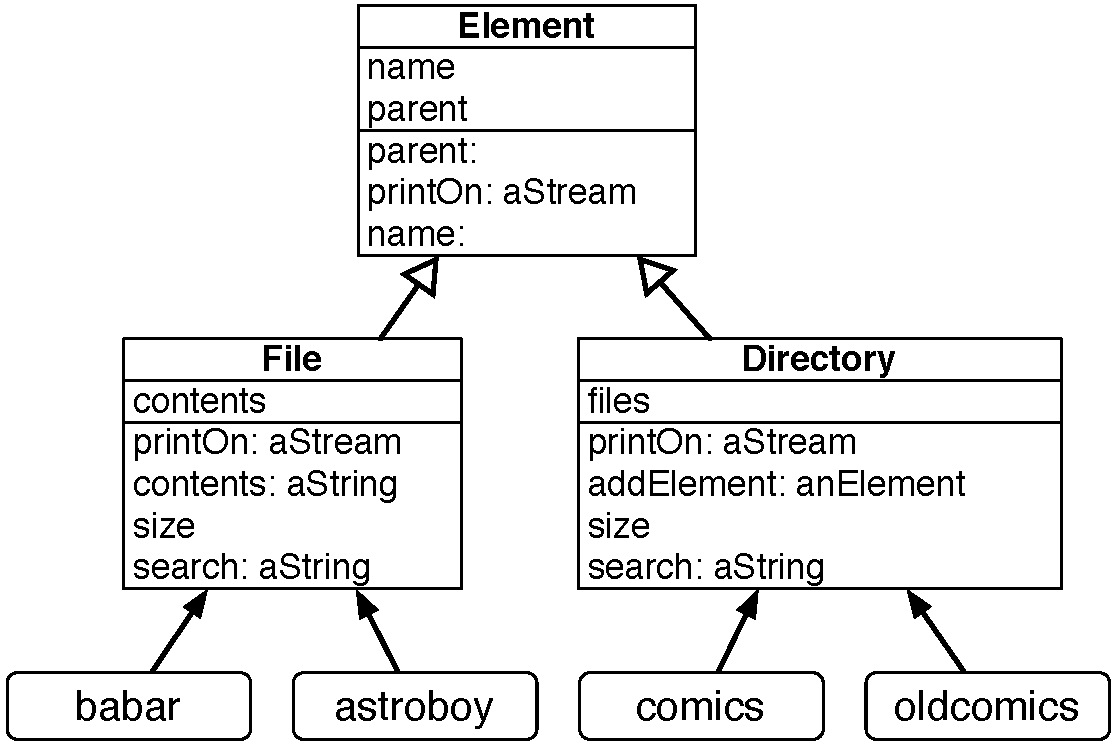
\includegraphics[width=0.6\textwidth]{/Users/ducasse/Workspace/FirstCircle/MyBooks/Bk-Writing/PharoBooks/LearningOOPWithPharoTrans/_result/pdf/Chapters/Inheritance/figures/FileDirectoryWithInheritanceObjective.pdf}\caption{Two class taking advantages of inheriting from a common superclass.\label{FileDirectoryWithInheritanceObjective}}\end{center}
\end{figure}

\section{Transformation strategies}
Let us define a new class called \textcode{MFElement}. 

\begin{displaycode}{plain}
Object subclass: #MFElement
	instanceVariableNames: ''
	classVariableNames: ''
	package: 'MyFS2'
\end{displaycode}

As you may noticed it, this class is empty. Now we have two possible strategies: 

\begin{itemize}
\item either we make \textcode{MFFile} and \textcode{MFDirectory} inherit from \textcode{MFElement} and  step by step we migrate the common state and behavior to the superclass,
\item or we define new state and behavior in \textcode{MFElement} and we remove it  from the two classes and when ready we make them inherit from \textcode{MFElement}. 
\end{itemize}

The second approach may work but it is too risky. Indeed with the first approach we can get a running system after any step we perform: why? Because we first inherit from the new class and move element from the subclasses to the classes and doing so we automatically reuse the superclass behavior and state so our program externally (for example from the test perspective) is not changed. With such an approach we can run our tests after any change and control our enhancements.

In addition, some of the operations such as moving an instance variable from a class to its superclass are tedious to perform. Here we will perform one operation manually but for the rest of the changes we will use \textit{refactorings} -- refactorings are program transformations that keep the behavior of the program the same.

Let us get started.
\section{Factoring out state}
The first step is to make \textcode{MFFile} and \textcode{MFDirectory} subclasses of \textcode{MFElement} as follows:

\begin{displaycode}{plain}
MFElement subclass: #MFFile
	instanceVariableNames: 'parent name contents'
	classVariableNames: ''
	package: 'MyFS2'
\end{displaycode}

\begin{displaycode}{plain}
MFElement subclass: #MFDirectory
	instanceVariableNames: 'parent name files'
	classVariableNames: ''
	package: 'MyFS2'
\end{displaycode}

Now you can execute the tests and they will all pass. Now we get ready move some instance variables to the superclass.


\begin{figure}

\begin{center}
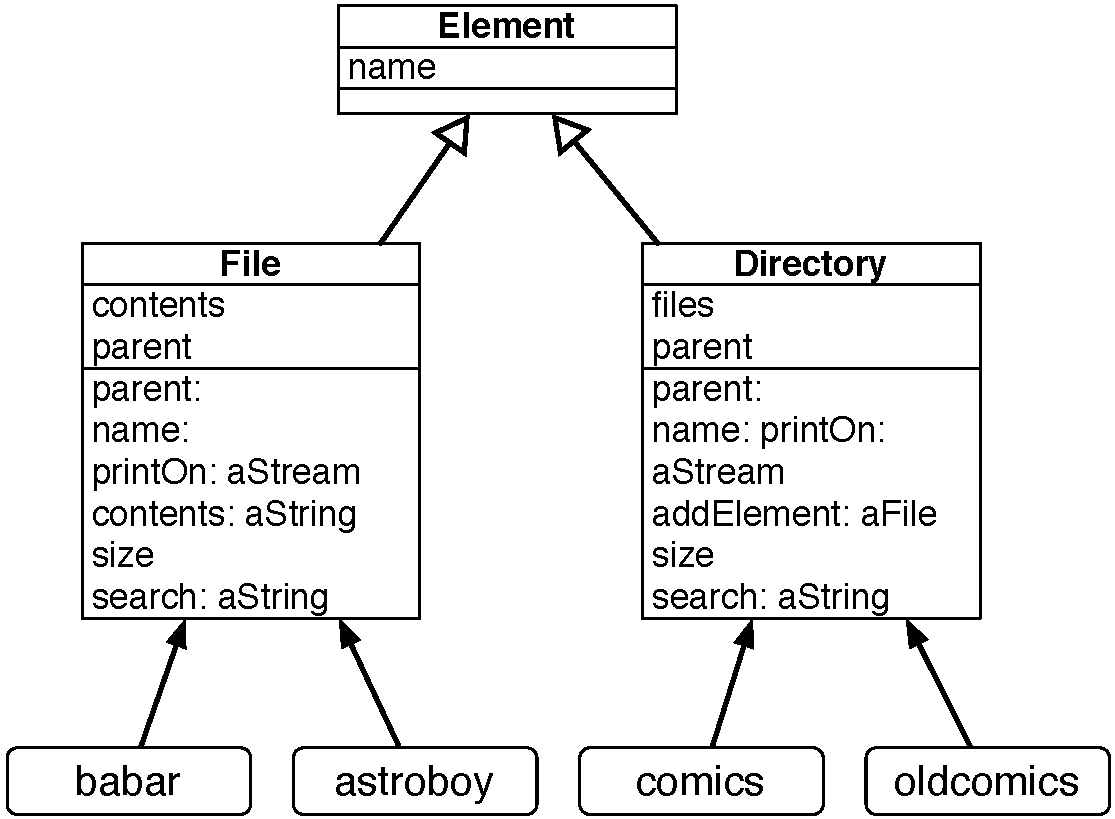
\includegraphics[width=0.5\textwidth]{/Users/ducasse/Workspace/FirstCircle/MyBooks/Bk-Writing/PharoBooks/LearningOOPWithPharoTrans/_result/pdf/Chapters/Inheritance/figures/FileDirectoryInhStateNameOnly.pdf}\caption{Moving the instance variable name to the superclass.\label{FileDirectoryInhStateNameOnly}}\end{center}
\end{figure}

\subsection{Moving instance variable name to superclass}
Since both \textcode{MFDirectory} and \textcode{MFFile} define that their instances should have a name, we can remove the instance variable \textcode{name} from them and uniquely define it in the superclass. We obtain the situation depicted in Figure \ref{FileDirectoryInhStateNameOnly}.
Let us do that as follows: We remove it first from the \textcode{MFFile} and \textcode{MFDirectory} classes.

\begin{displaycode}{plain}
MFElement subclass: #MFFile
	instanceVariableNames: 'parent contents'
	classVariableNames: ''
	package: 'MyFS2'
\end{displaycode}

\begin{displaycode}{plain}
MFElement subclass: #MFDirectory
	instanceVariableNames: 'parent files'
	classVariableNames: ''
	package: 'MyFS2'
\end{displaycode}

And we add the instance variable \textcode{name} to the superclass \textcode{MFElement}.

\begin{displaycode}{plain}
Object subclass: #MFElement
	instanceVariableNames: 'name'
	classVariableNames: ''
	package: 'MyFS2'
\end{displaycode}

Pay attention that you should be careful and do it in this order else you may be in the situation where name will be defined in the superclass and in one of the subclasses and the system does not allow this and will forbid your action. 

Again run the tests they should pass again. 

What the tests execution proves is that we did not change the structure of the instances of \textcode{MFFile} and \textcode{MFDirectory}. Indeed the structure of an instance is computed from the instance variable lists defined in their class and all the superclasses of that class.
\subsection{Moving parent to superclass}
Since parent is defined in both subclasses, we can do the same for the instance variable parent to obtain the situation shown in Figure \ref{FileDirectoryInhFullStateOnly}.
You can do it manually, as we did for the instance variable \textcode{name}, but you can also use a \textit{refactoring}: Refactorings are powerful program transformations. Using the system browser, bring the menu on the class \textcode{MFFile}, select refactoring, then the instance variable category, and finally pull up, as shown in Figure \ref{Refactoring}.


\begin{figure}

\begin{center}
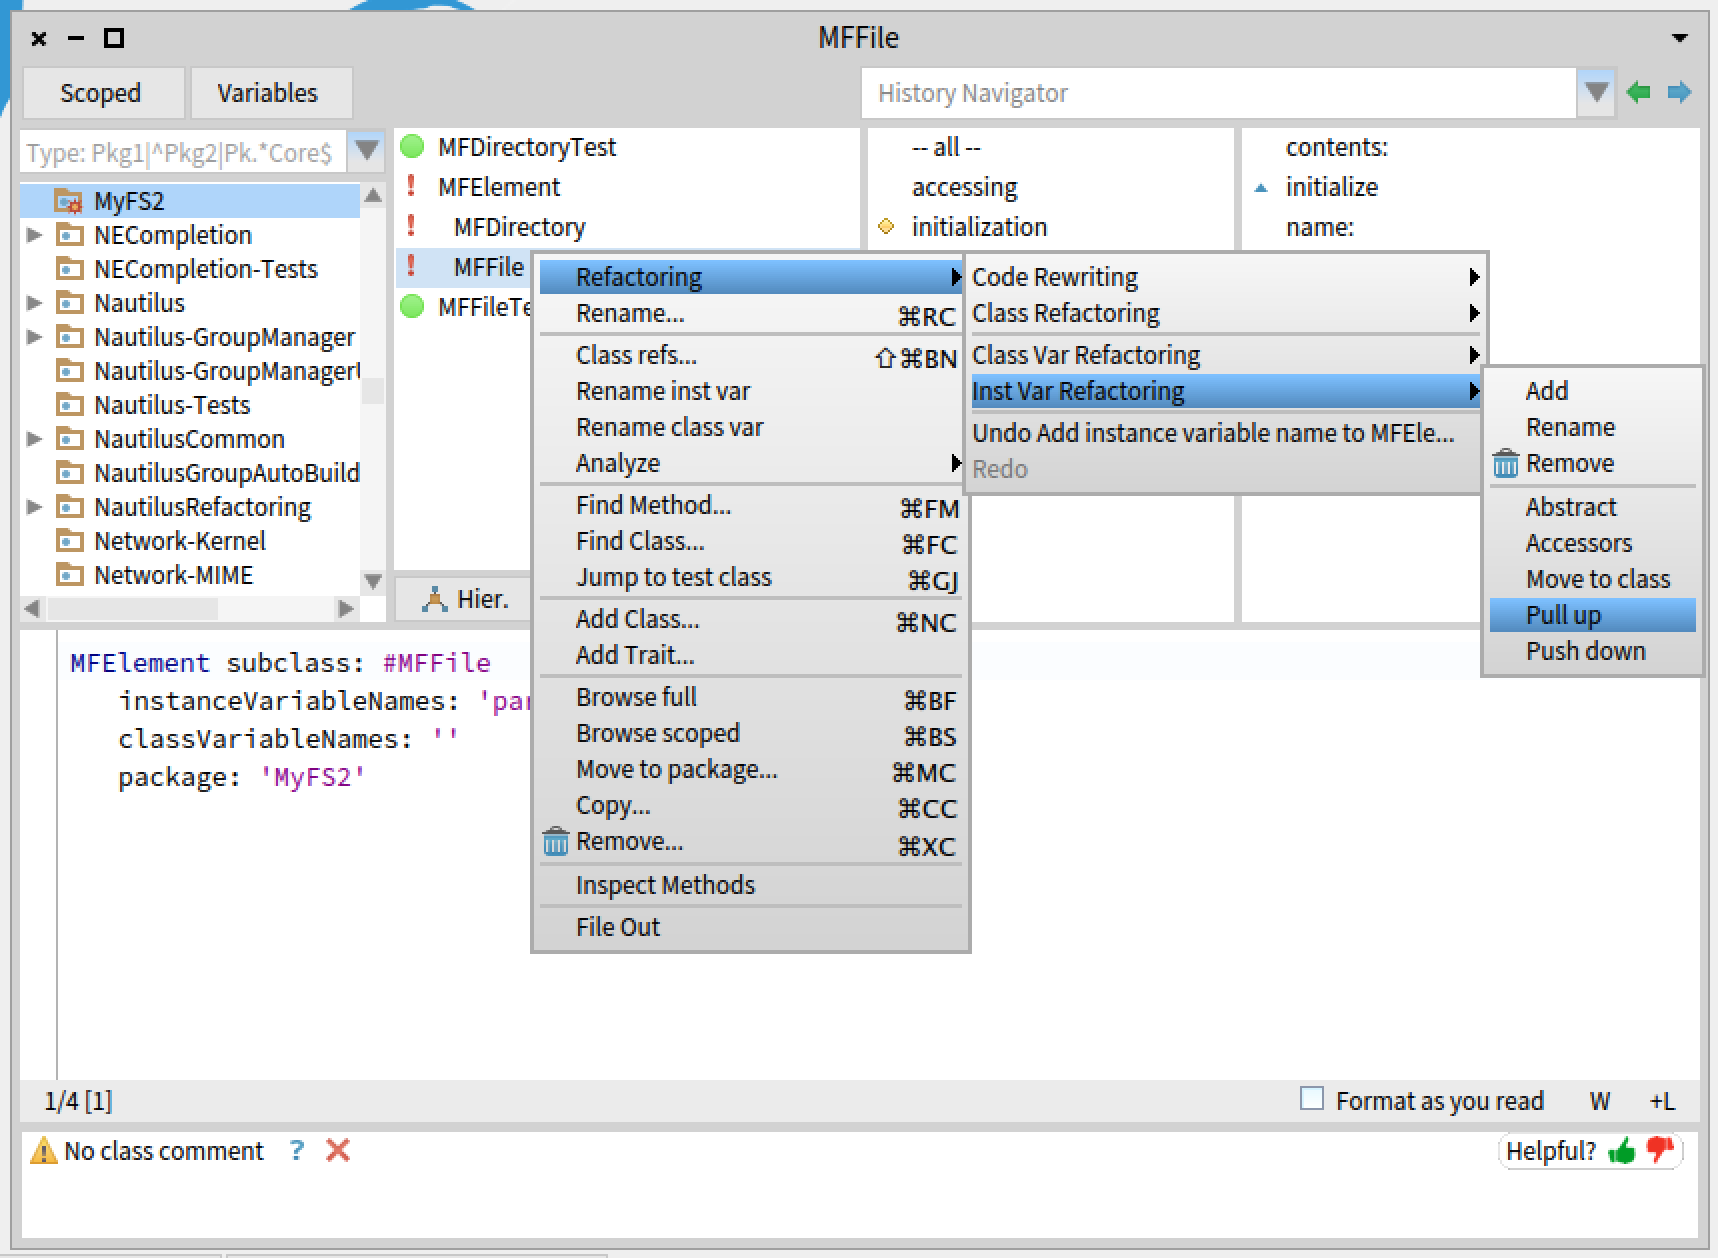
\includegraphics[width=0.6\textwidth]{/Users/ducasse/Workspace/FirstCircle/MyBooks/Bk-Writing/PharoBooks/LearningOOPWithPharoTrans/_result/pdf/Chapters/Inheritance/figures/Refactoring.png}\caption{Applying the Pull Up Instance variable refactoring.\label{Refactoring}}\end{center}
\end{figure}


The system will ask you which variable you want to pull up, select \textcode{parent}. It will show you the changes that it is about to perform: removing the instance variable from both subclasses and adding one to the superclass. Proceed and the changes will be executed. Your
code should be now in the situation depicted in Figure \ref{FileDirectoryInhFullStateOnly}.
Run the tests and they should again all pass!


\begin{figure}

\begin{center}
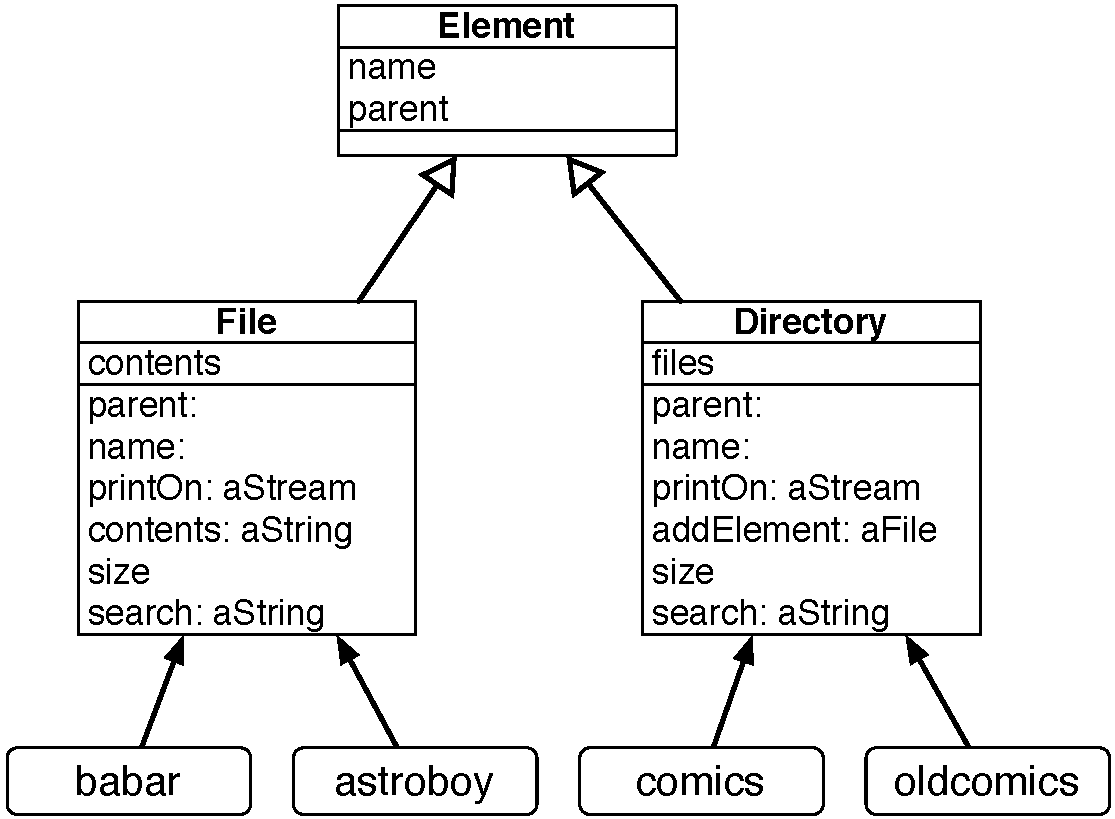
\includegraphics[width=0.5\textwidth]{/Users/ducasse/Workspace/FirstCircle/MyBooks/Bk-Writing/PharoBooks/LearningOOPWithPharoTrans/_result/pdf/Chapters/Inheritance/figures/FileDirectoryInhFullStateOnly.pdf}\caption{State factored between the two classes and their superclass.\label{FileDirectoryInhFullStateOnly}}\end{center}
\end{figure}


What is important to see is that if we create a new subclass of \textcode{MFElement}, the instances of such class will automatically get \textcode{name} and \textcode{parent} as instance variables. This is one of the key property of inheritance: you can define a new abstraction structure by extending an existing one. 

Now we can do the same for the behavior: we will move similar methods in the superclass and remove them from their respective classes. 
\section{Factoring similar methods}
The methods \textcode{parent:}, \textcode{parent} and \textcode{name:} are the same and defined in the two classes \textcode{MFFile} and \textcode{MFDirectory}. We will move them to the superclass \textcode{MFElement} following a similar process.

\begin{itemize}
\item First we will remove the method \textcode{name:} from the two classes \textcode{MFFile} and \textcode{MFDirectory} and add one version to the class \textcode{MFElement}. You can do this manually. 
\end{itemize}

\begin{itemize}
\item Second for the method \textcode{parent:}, use the method Refactoring \textit{Push Up Method} that is available from the method list.  You can repeat this for the method \textcode{parent} too. 
\end{itemize}

You should obtain the system described in Figure \ref{FileDirectoryInhAccessors}.


\begin{figure}

\begin{center}
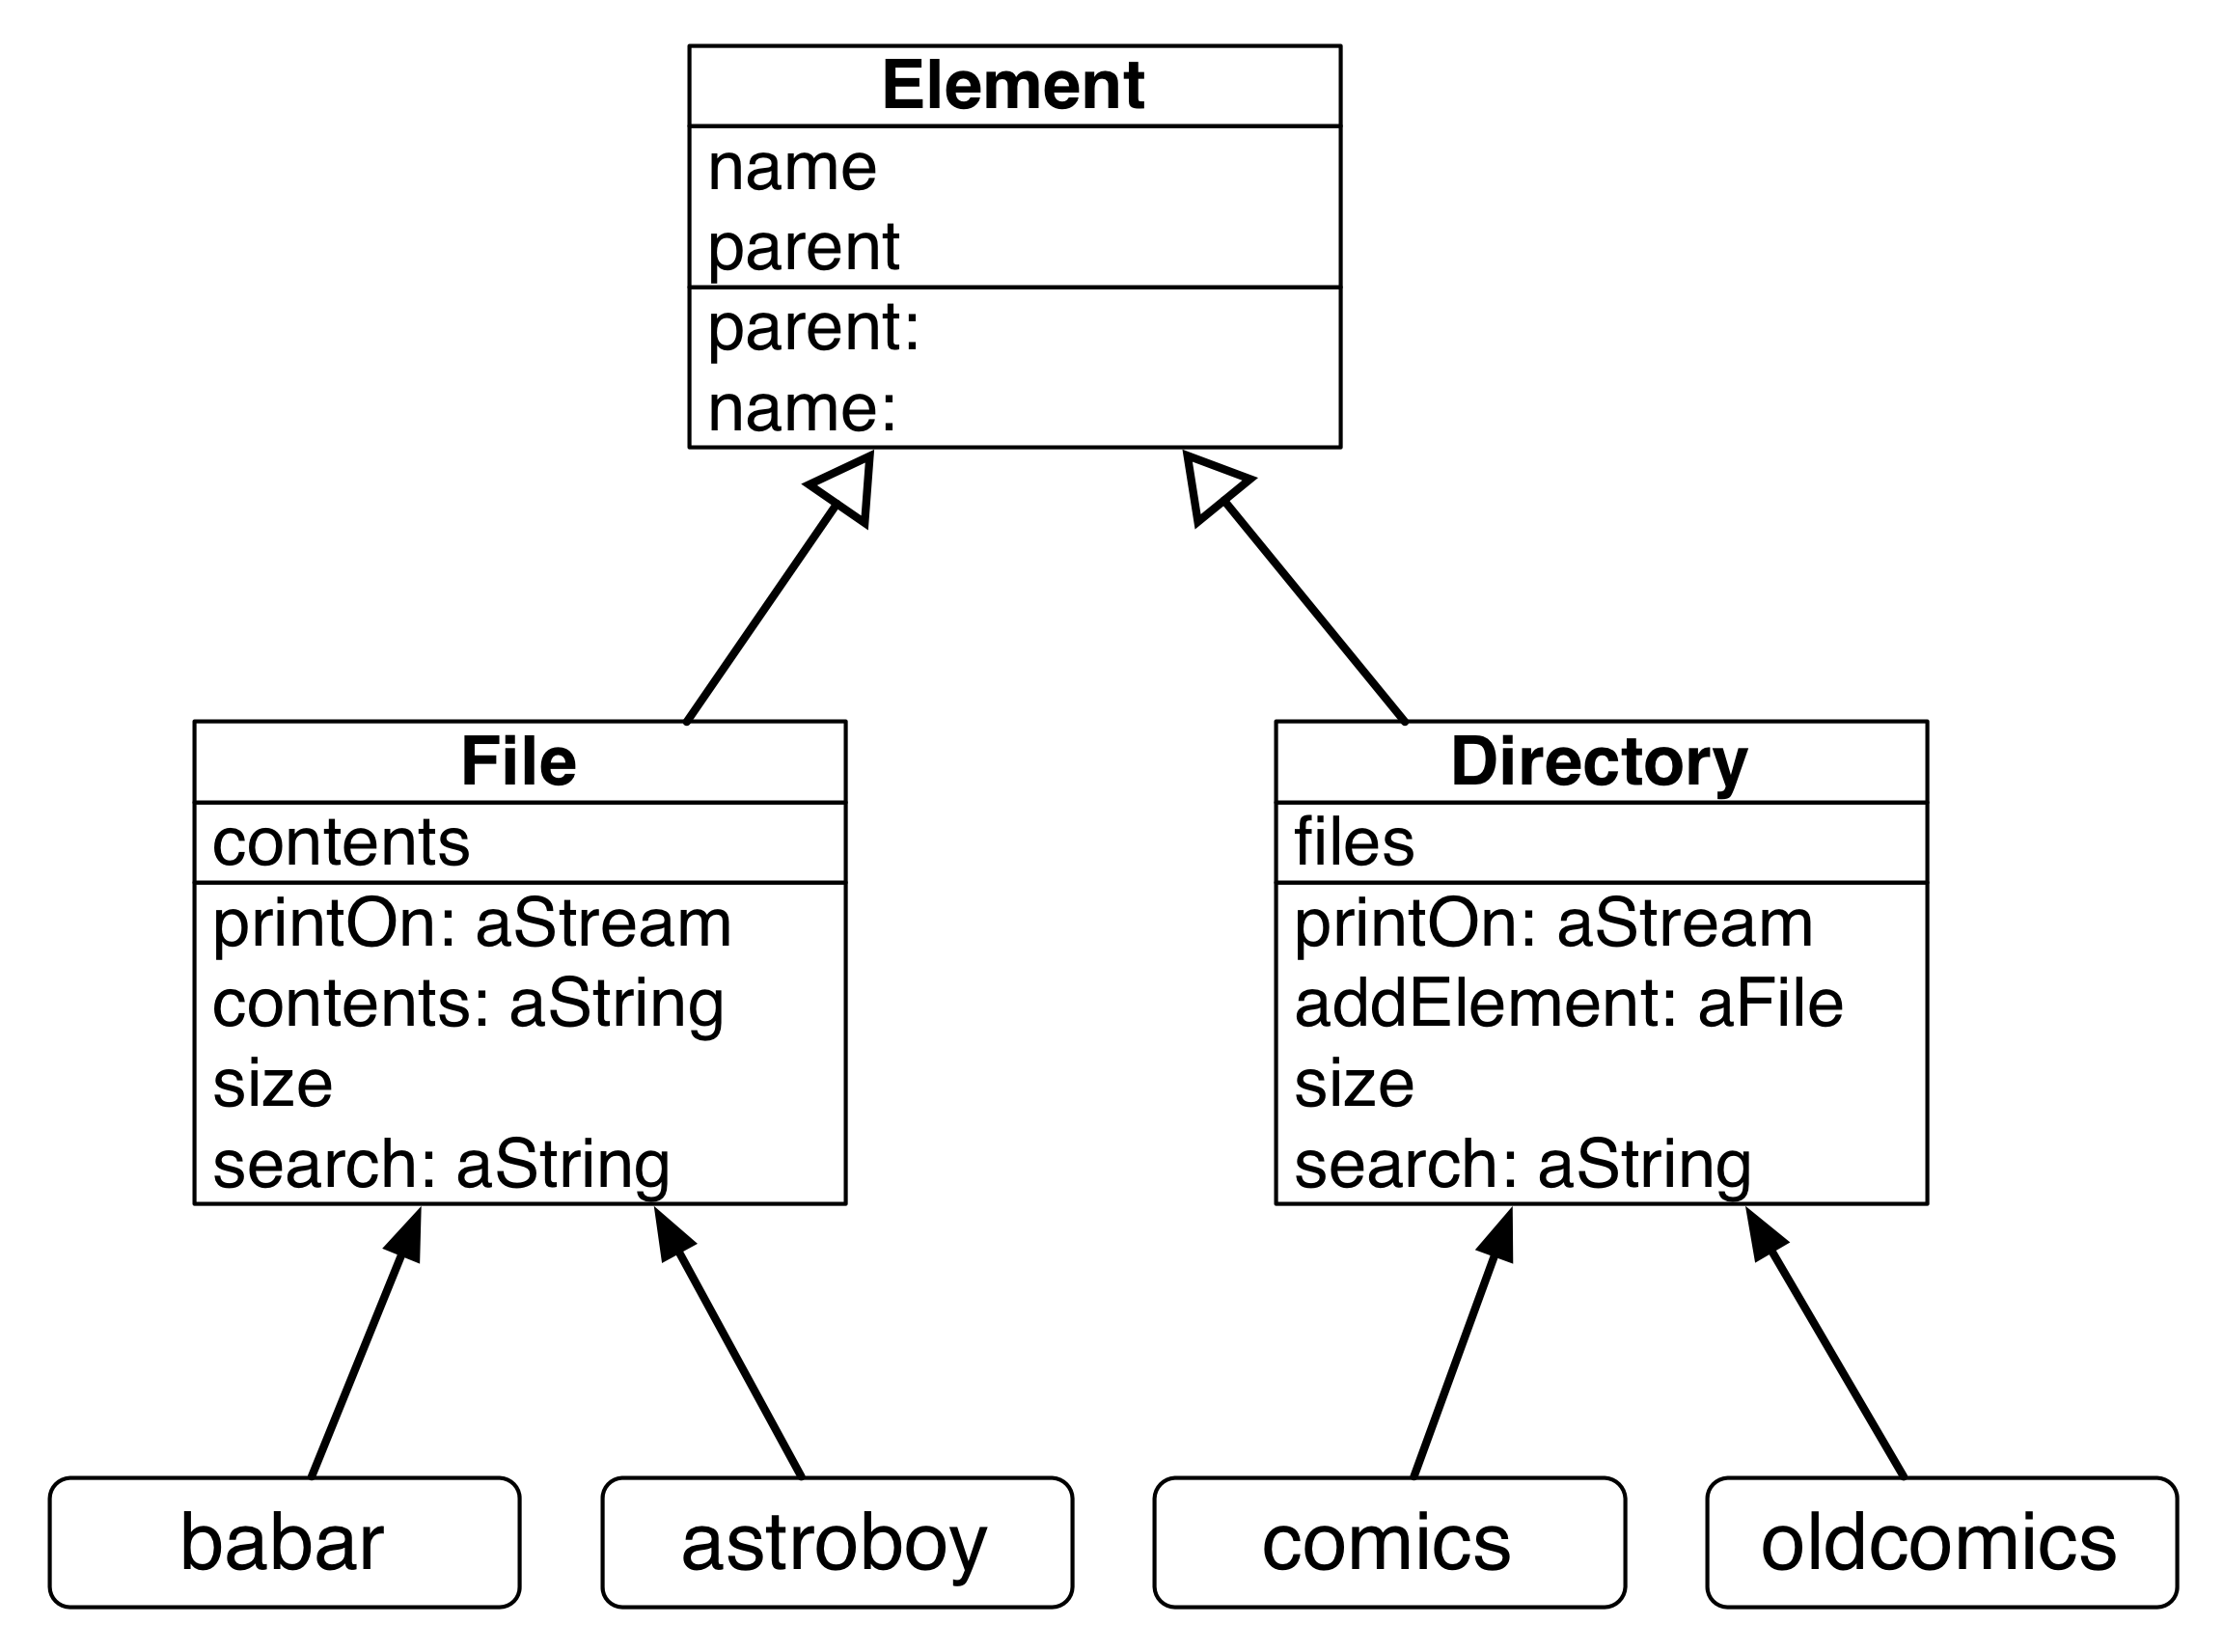
\includegraphics[width=0.5\textwidth]{/Users/ducasse/Workspace/FirstCircle/MyBooks/Bk-Writing/PharoBooks/LearningOOPWithPharoTrans/_result/pdf/Chapters/Inheritance/figures/FileDirectoryInhAccessors.png}\caption{ State and Methods factored out in the superclass.\label{FileDirectoryInhAccessors}}\end{center}
\end{figure}


Again run the tests and they should all pass. Why? Let us see what is happening when we send a message.
\section{Sending a message and method lookup }

\begin{figure}

\begin{center}
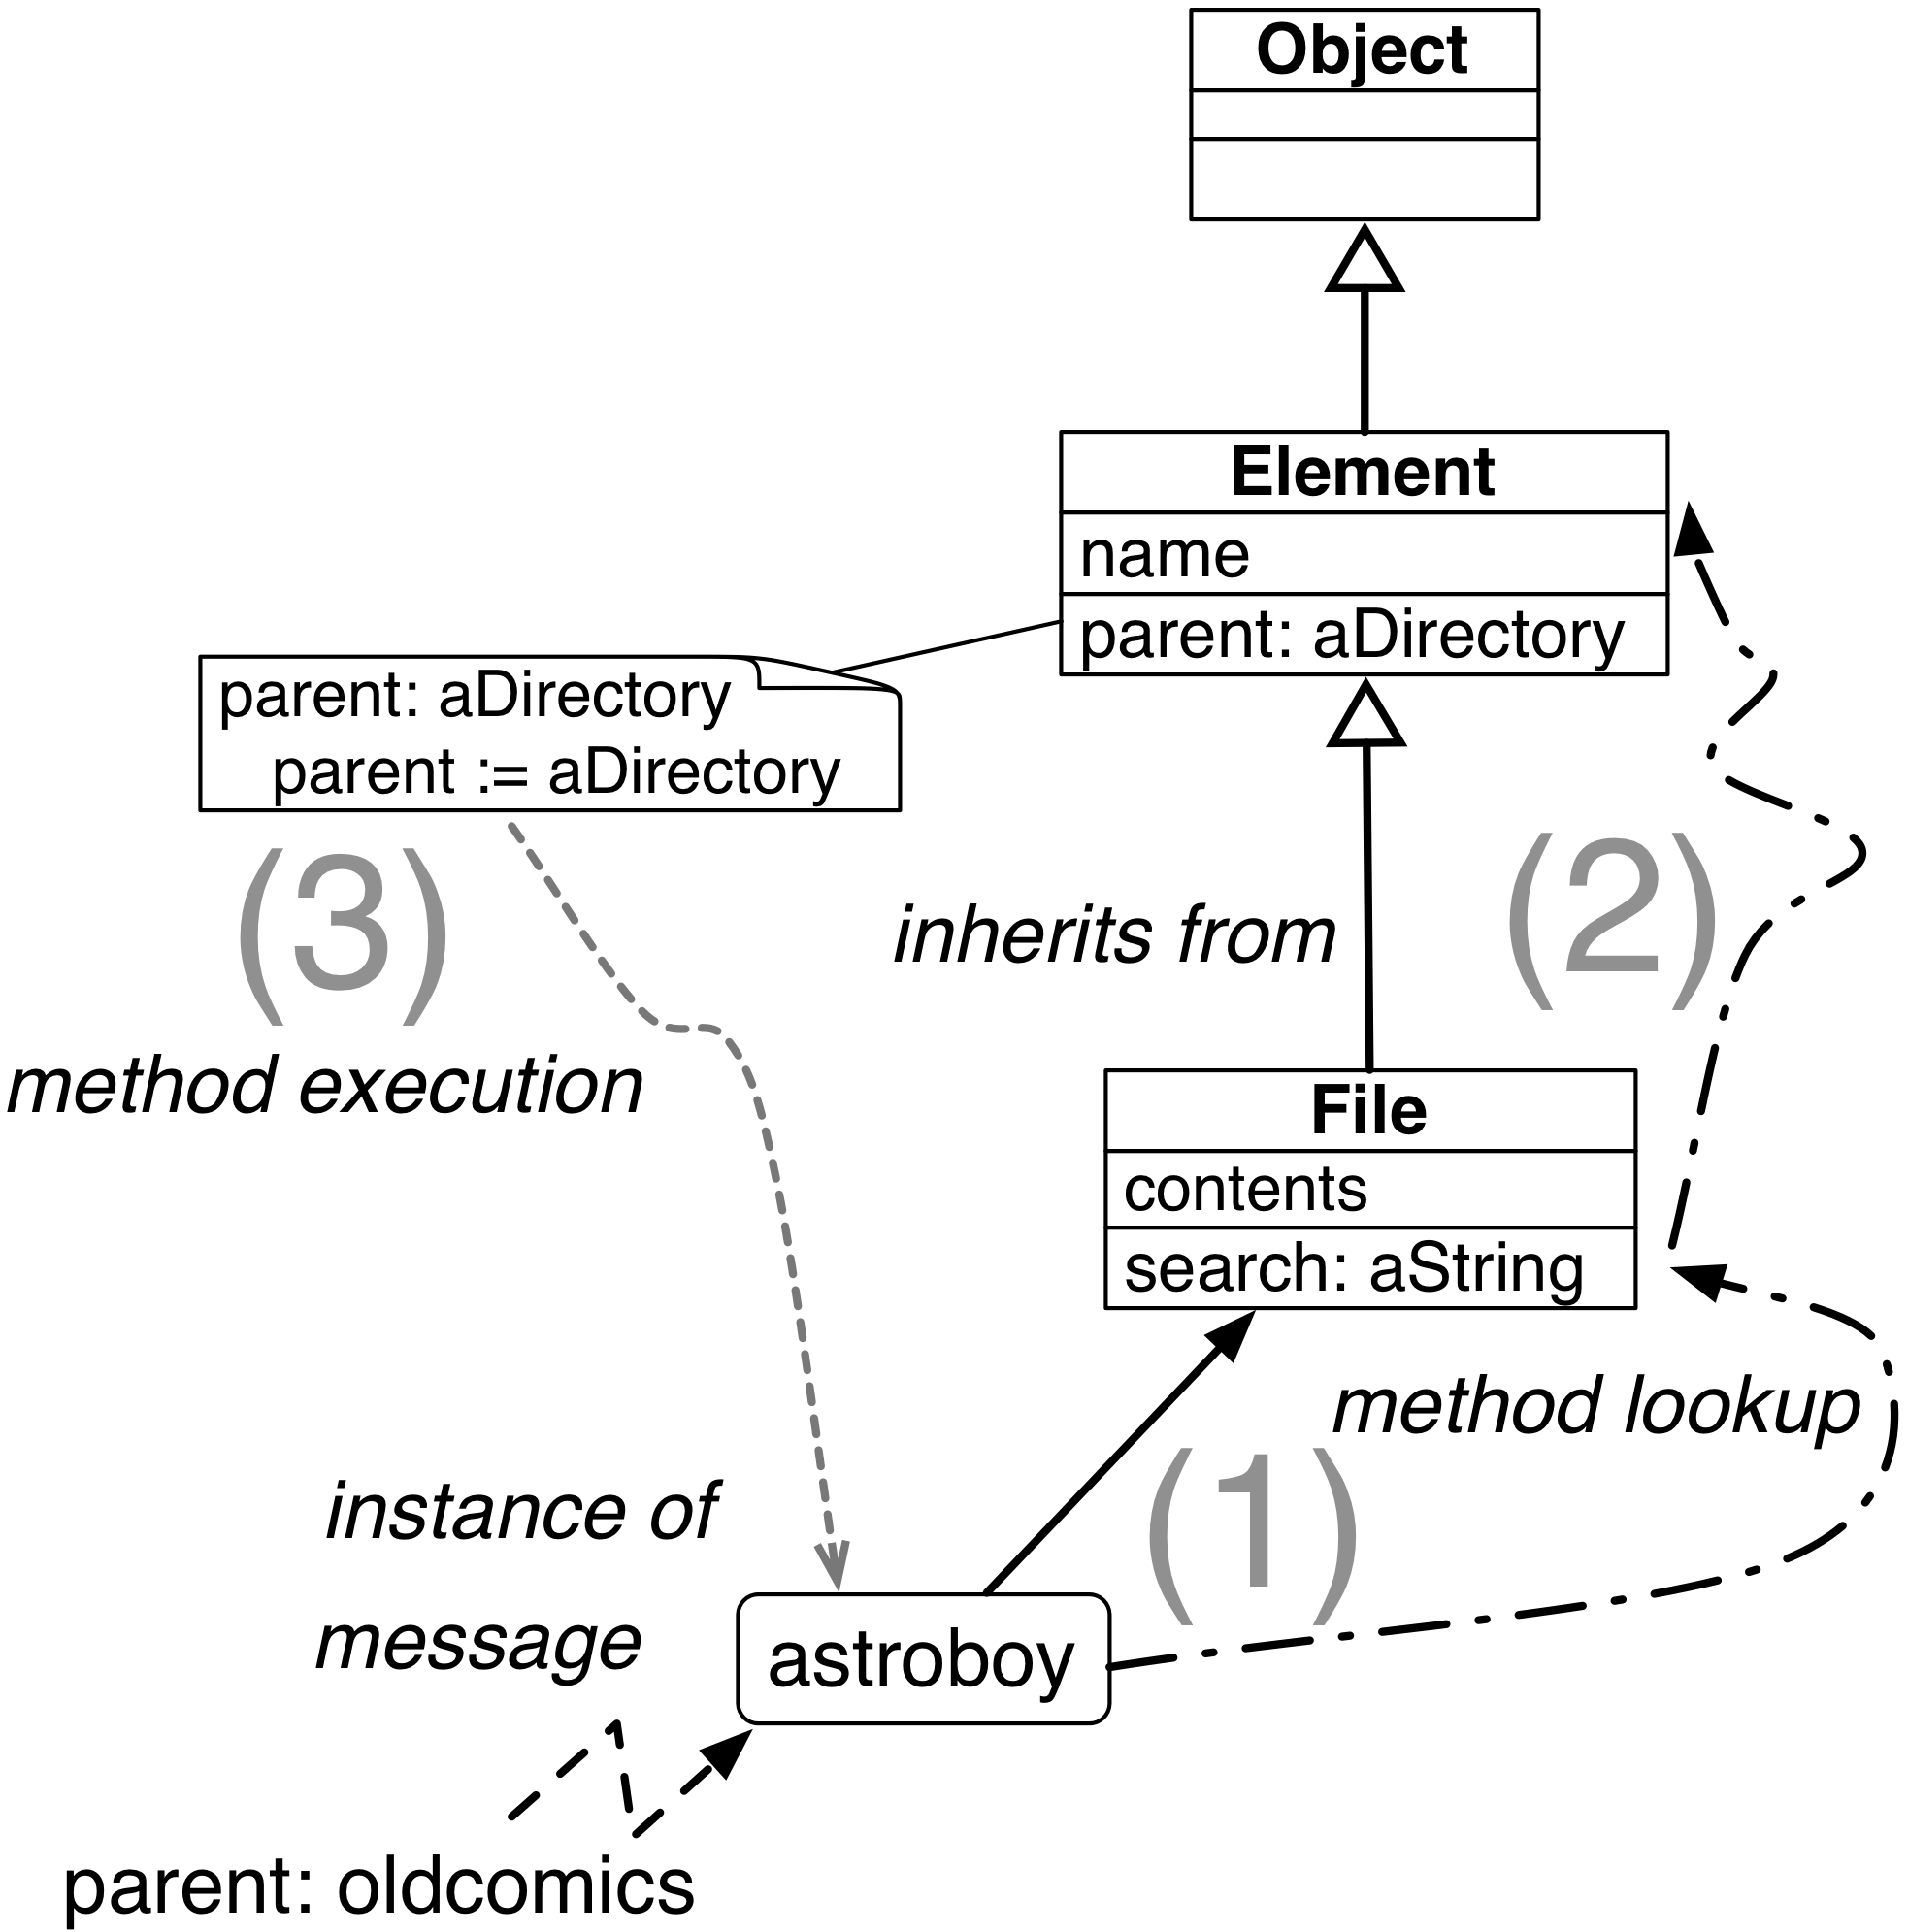
\includegraphics[width=0.5\textwidth]{/Users/ducasse/Workspace/FirstCircle/MyBooks/Bk-Writing/PharoBooks/LearningOOPWithPharoTrans/_result/pdf/Chapters/Inheritance/figures/BasicLookupAndExecution.png}\caption{When an object receives a message, the corresponding method is looked up in its class and if necessary its superclasses (Step 1 and 2). Then the method is executed on the message receiver (Step 3).\label{BasicLookup}}\end{center}
\end{figure}


Now it is time to explain what is happening when an object receives a message. In fact this is really simple but extremely powerful. When a message is sent to an object, first the corresponding method is looked up and once the method is found, it is executed on the object that initially received the message. 

\begin{itemize}
\item \textbf{Method Lookup}. When an object, the message receiver, receives a message, the method with the same selector than the message is looked up starting from the \textit{class} of receiver (See step 1 in Figure \ref{BasicLookup}). When there is no method with the same selector, the look up continues in the superclass of the current class (See step 2 in Figure \ref{BasicLookup}).
\item \textbf{Method execution}. When a method with the same selector is found in a class, it is returned and executed on the receiver of the message (See step 3 in Figure \ref{BasicLookup}). 
\end{itemize}

Let us look at our example. 

\begin{itemize}
\item When we send the message \textcode{astroboy parent: oldcomics}, the method named \textcode{parent:} is looked up in the class of the receiver i.e., \textcode{MFFile}. This class defines such a method, so it is returned and executed on the file \textcode{astroboy}.
\end{itemize}

\begin{itemize}
\item The tests pass because when we send the message \textcode{parent:} to an instance of the class \textcode{MFFile}, the corresponding method is looked up in the class \textcode{MFFile}. Since there is no method \textcode{parent:} in the class \textcode{MFFile}, the lookup continues in the superclass and find it in the class \textcode{MFElement} as shown in Figure \ref{BasicLookup}.
\end{itemize}
\subsection{Inheritance properties}
While rather simple, the previous example shows some key properties of inheritance. 

Inheritance is a mechanism to define abstraction incrementally: a subclass is defined by expressing the difference to its superclass. A subclass refines a general concept into a more specific one. The classes \textcode{MFFile} and \textcode{MFDirectory} add extra behavior and state to the one defined in the superclass. As such they reuse the state and behavior of their superclass.

\begin{itemize}
\item \textit{State reuse}: instances of a subclass have at least the structure of their superclasses (\textcode{name} and \textcode{parent}), local state can be added in addition (\textcode{contents} and \textcode{files}).
\end{itemize}

\begin{itemize}
\item \textit{Behavior reuse}: when instances of a subclass receive a message, methods of the superclass may be executed. The method \textcode{parent:}, \textcode{parent}, and \textcode{name} are defined in \textcode{MFElement} but are executed on instances of the subclasses.
\end{itemize}

Inheritance creates trees of refined concepts. A superclass represents a more abstract concepts and its subclasses make it more and more specific by refining the superclass behavior or extending it by adding new behavior. 
\section{Basic method overrides}
Since the method lookup starts from the class of the receiver, redefining a method in subclass takes precedence over the method defined in the superclasses.

If we define a method with the same name that one of its superclass, this new method will be executed instead of the one in the superclass. This is called a \textit{method override}. This is useful to be able to redefine locally a behavior taking advantage of the specificities of the subclasses. In Figure \ref{BasicLookup}, if we add a new method named \textcode{parent:} in the class \textcode{MFFile}, this method will be executed when the message \textcode{parent:} is sent to an instance of the class \textcode{File}. 

We will see later that we can also invoke the method of the superclass while doing a method overrides: it is useful when we want to \textit{extend} and not just fully change the superclass behavior. 

But before explaining this, method lookup and execution are systematically applied and we will see in the following sections that it is even more powerful than it may look at first sight.
\section{self-send messages and lookup create hooks}
So far we explained how a message is resolved: first the corresponding method is looked up from the class of the receiver and goes up the inheritance tree. Second, the found method is executed on the message receiver. It means that in response to a message, a superclass method may be executed on its subclass instances. This is the same for message sent to \textcode{self} (the receiver of the message), we invoke the method lookup and \textcode{self} may be one subclass instances.

There is an important implication: when we have a message sent to \textcode{self} in a method, this message may lead to the execution of a method defined in subclasses: because a subclass may override such method. This is why self-sends are also called \textit{hooks} methods. We will explain carefully this point. 
\subsection{Example}
To explain precisely this important point, let us define a new little behavior: to build a better user interface for end-users we add a new message called \textcode{describe} that presents in more human friendly way the receiver of the message.
Here is a small example: 

\begin{displaycode}{plain}
| p el1 el2 |
p := MFDirectory new name: 'comics'.
el1 := MFFile new name: 'babar'; contents: 'Babar et Celeste'.
p addElement: el1.
el2 := MFFile new name: 'astroboy'; contents: 'super cool robot'.
p addElement: el2.
p describe
>>> 'I m a directory named comics'
el1 describe
>>> 'I m a file named babar'
\end{displaycode}
\subsection{Describe implementation }
We implement now the situation described by Figure \ref{fig:SelfSendLateBinding}.
To implement this behavior, we define the following method \textcode{describe} in the class \textcode{MFElement}.

\begin{displaycode}{plain}
MFElement >> describe
	^ 'I m a ', self kind, 'named ', name  
\end{displaycode}

We define the method \textcode{kind} to return a default string, even though we do not expect 
to create instances of this class and subclasses should define their own definition.

\begin{displaycode}{plain}
MFElement >> kind
	^ 'element'
\end{displaycode}

In each of the subclasses, we define a corresponding method \textcode{kind}, as follows: 

\begin{displaycode}{plain}
MFDirectory >> kind
	^ 'directory'
\end{displaycode}

\begin{displaycode}{plain}
MFFile >> kind
	^ 'file'
\end{displaycode}
\section{Hook/Template explanations}
Now we are ready to explain what is happening. Let us illustrate the execution of the \textcode{(MFFile new name: 'astroboy') describe}.

\begin{displaycode}{plain}
| el1 |
el1 := (MFFile new name: 'astroboy').
el1 describe
>>> 'I m a file named astroboy'
\end{displaycode}

The following steps are executed: 

\begin{itemize}
\item The message \textcode{describe} is sent to \textcode{el1} an instance of the class \textcode{MFFile}. 
\item The method \textcode{describe} is looked up in the class \textcode{MFFile} (step 1 in Figure \ref{fig:SelfSendLateBinding}). It is not found, therefore the lookup continues to the superclass. 
\item The lookup looks for the method \textcode{describe} in the class \textcode{MFElement}  (step 2 in Figure \ref{fig:SelfSendLateBinding}). It is found and executed on the receiver: \textcode{el1}. 
\item During the execution of the method \textcode{describe}, a new message \textcode{kind} using the expression \textcode{self kind} is sent (step 3 in Figure \ref{fig:SelfSendLateBinding}).
\item The message \textcode{kind} is looked up starting from the class of the receiver, \textcode{MFFile} (step 4 in Figure \ref{fig:SelfSendLateBinding}). The method \textcode{kind} is found in class \textcode{MFFIle} and executed. 
\item The rest of the method \textcode{describe} is executed and the resulting string is returned.
\end{itemize}


\begin{figure}

\begin{center}
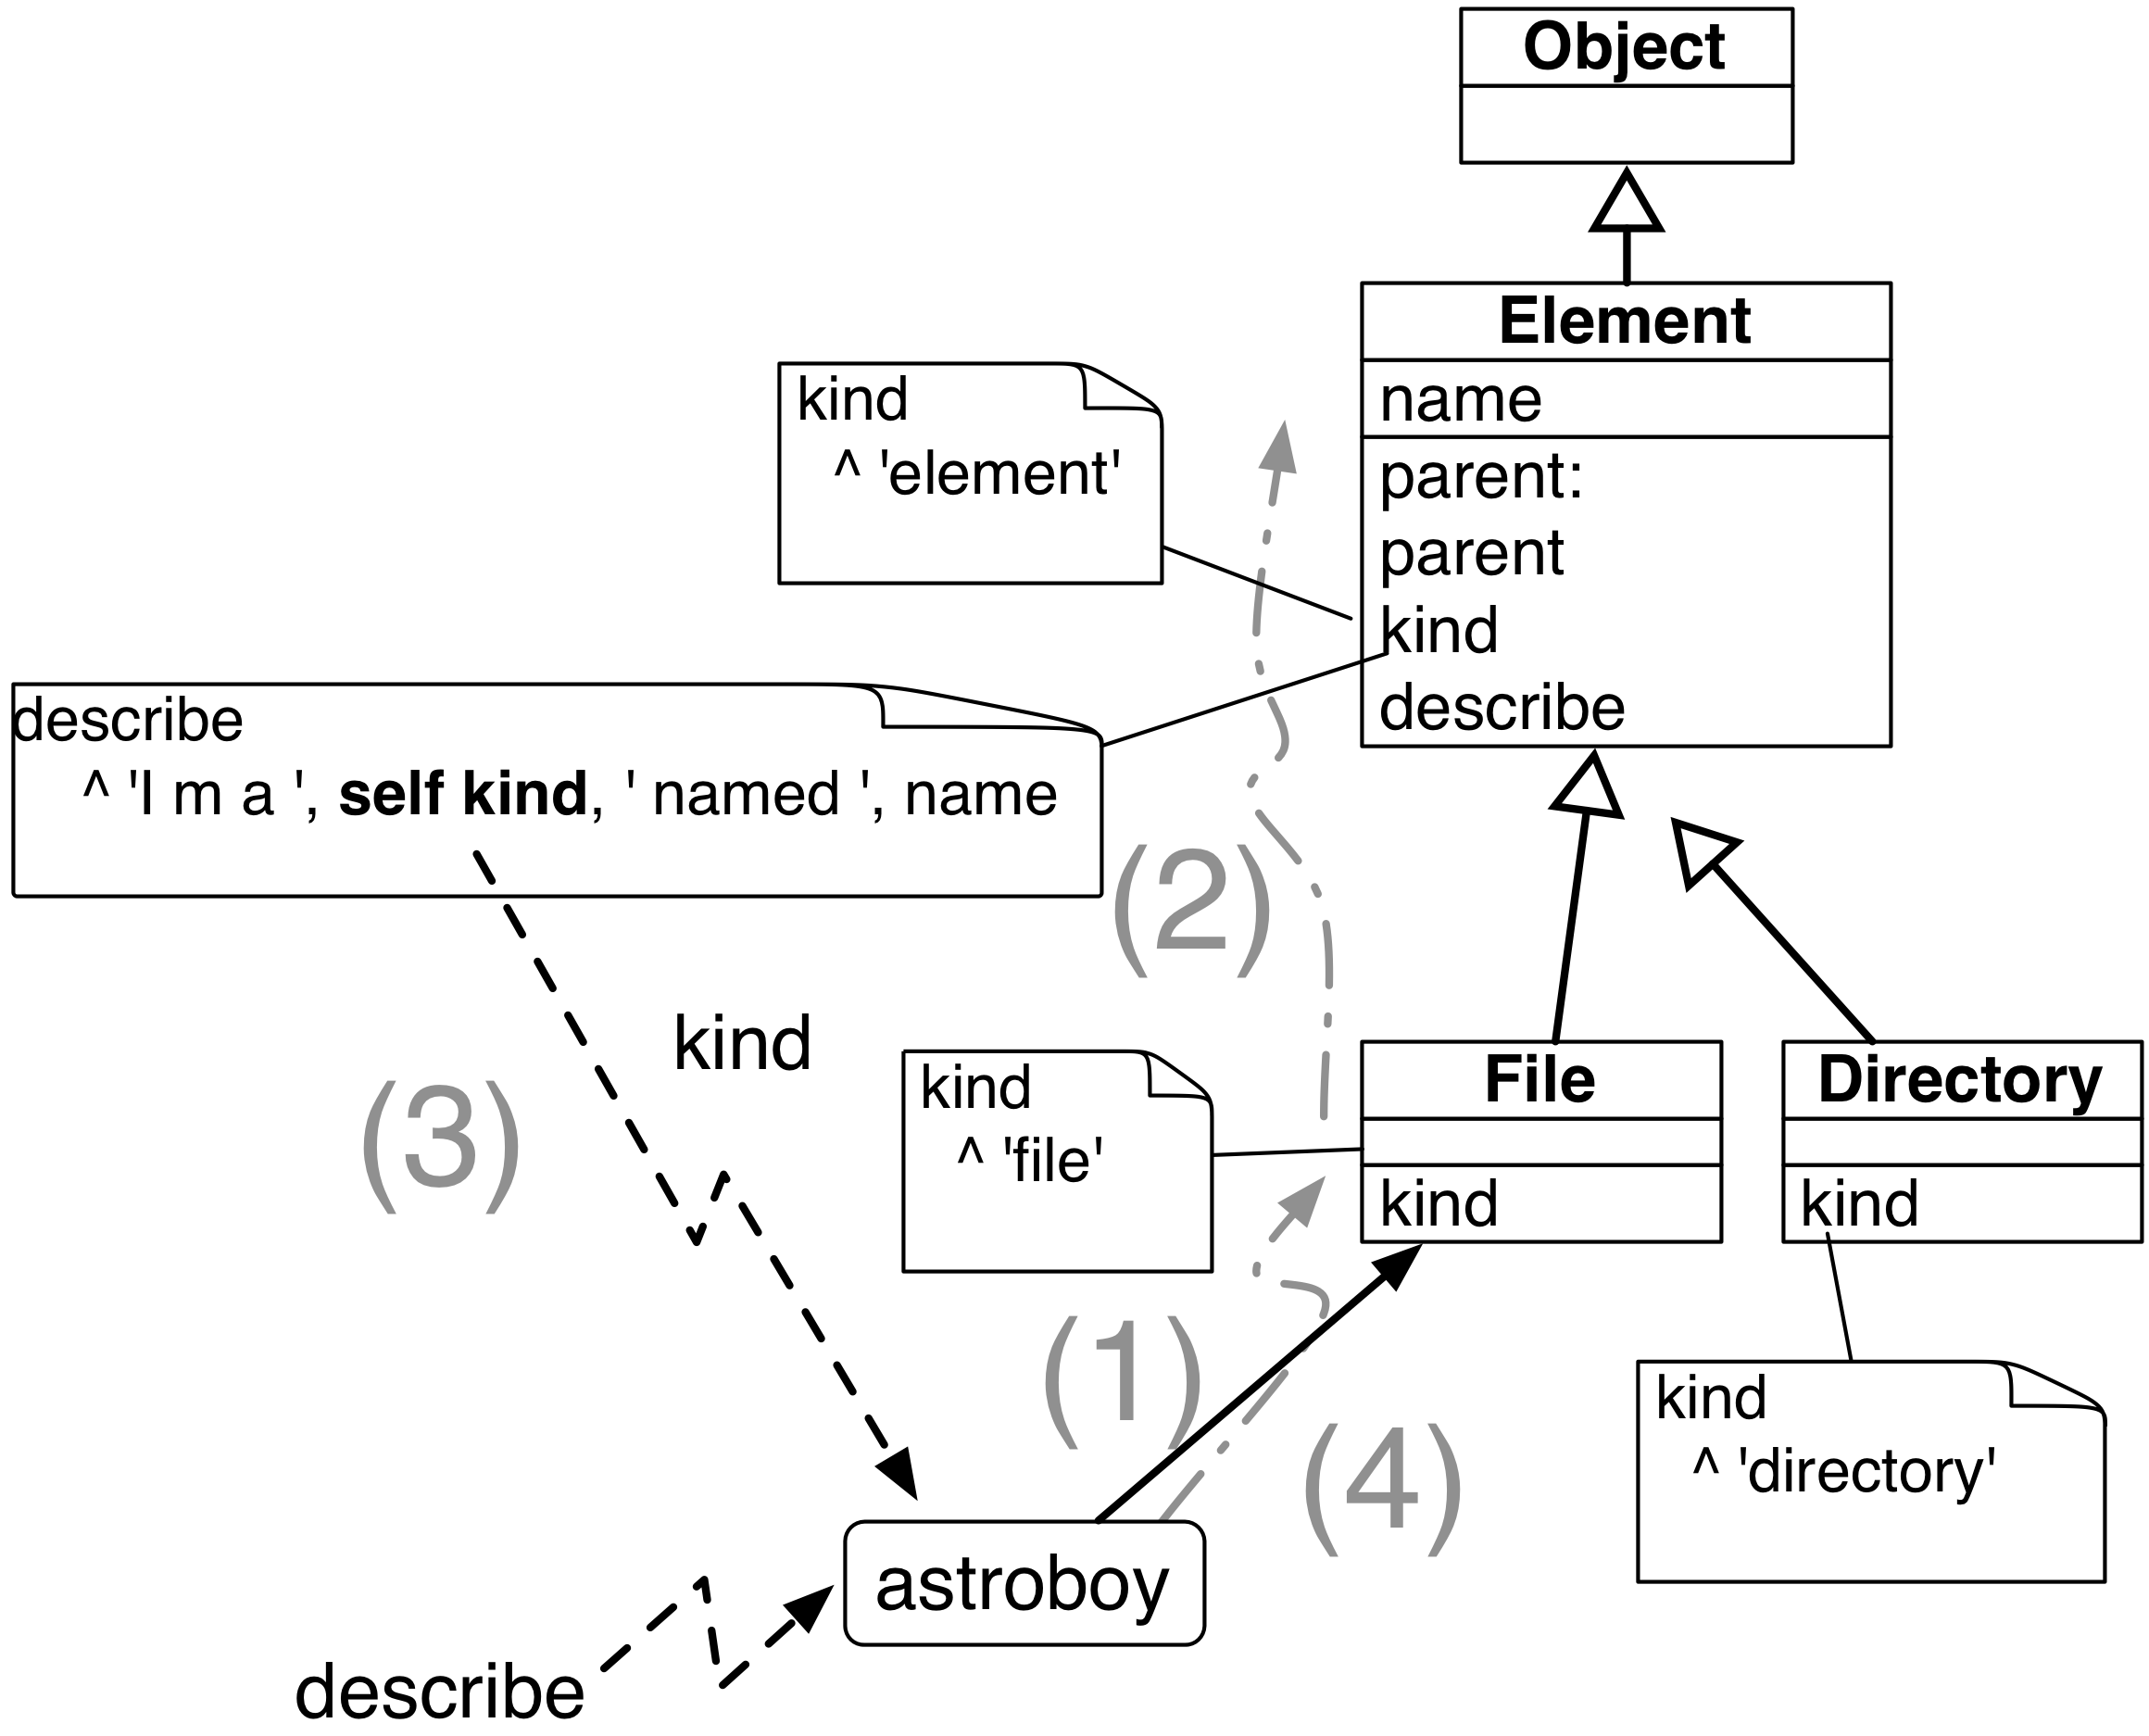
\includegraphics[width=0.65\textwidth]{/Users/ducasse/Workspace/FirstCircle/MyBooks/Bk-Writing/PharoBooks/LearningOOPWithPharoTrans/_result/pdf/Chapters/Inheritance/figures/SelfSendLateBinding.png}\caption{A self-send creates a hook (\textcode{kind}) that subclasses override. The method \textcode{ describe} is called a template because it creates a context.\label{fig:SelfSendLateBinding}}\end{center}
\end{figure}


A vocabulary point: the method \textcode{describe} is called a \textit{template} method because it creates a context in which the \textcode{kind} methods are executed. The message \textcode{kind} is called a hook since subclass implementation may be invoked in this place.

This example illustrates the following important points:

\begin{itemize}
\item Each time we send a message the system chooses the correct method to be executed.
\item Each time we send a self-send message we create a place where subclass methods may be executed. We create customization points.
\item Since \textcode{self} represents the receiver and that receiver may be an instance from a class that is not loaded at the time the method containing the self-send, we say that \textcode{self} is dynamic. It represents the receiver of the message and the lookup for the method to execute starts in the class of the receiver. 
\end{itemize}

\begin{important}
Messages sent to the receiver (\textcode{self} sends) define customization points that subclasses can take advantage of to potentially see their code being executed in place of the superclass' one.
\end{important}
\section{Essence of self and dispatch}
Now we take some time to look abstractly at what we presented so far. 
Imagine a situation as illustrated by Figure \ref{fig:LookupWithSelfInSuperclassMethod}.

The first questions are simple and should be not a problem for you. Without looking at the solutions guess what are the results of the following messages.

\begin{displaycode}{plain}
A new foo
>>> ... 
B new foo
>>> ...
\end{displaycode}

What is more interesting is the process to get the result of \textcode{B new bar}.

\begin{displaycode}{plain}
A new bar
>>> ...
B new bar
>>> ...
\end{displaycode}


\begin{figure}

\begin{center}
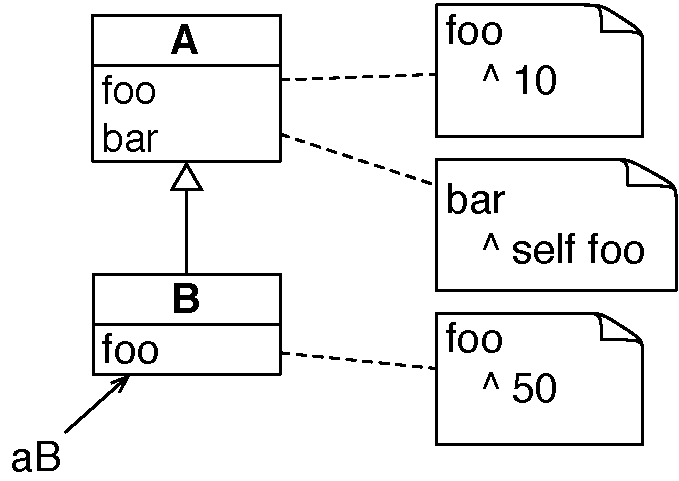
\includegraphics[width=0.35\textwidth]{/Users/ducasse/Workspace/FirstCircle/MyBooks/Bk-Writing/PharoBooks/LearningOOPWithPharoTrans/_result/pdf/Chapters/Inheritance/figures/LookupWithSelfInSuperclassMethod.pdf}\caption{Self semantics abstractly explained.\label{fig:LookupWithSelfInSuperclassMethod}}\end{center}
\end{figure}

\subsection{Solutions}
The solutions are the following ones.

\begin{displaycode}{plain}
A new foo
>>> 10

B new foo
>>> 50

A new bar
>>> 10

B new bar
>>> 50
\end{displaycode}

The most interesting one is \textcode{B new bar}.  Let us look at the execution of \textcode{aB bar}

\begin{enumerate}
\item \textcode{aB}'s class is \textcode{B}.
\item The method look up starts in the class \textcode{B}.
\item There is no method \textcode{bar} in \textcode{B}.
\item The look up continues in \textcode{A} and method \textcode{bar} is found.
\item The method \textcode{bar} is executed on the receiver  \textcode{aB}.
\item \textcode{self} refers to the receiver \textcode{aB}.
\item The message \textcode{foo} is sent to \textcode{self}.
\item The look up of \textcode{foo} starts in the \textcode{aB}'s class: \textcode{B}.
\item The method \textcode{foo} is found in class \textcode{B} and executed on the receiver \textcode{aB}.
\end{enumerate}

\begin{important}
\textcode{self} represents the receiver. Messages sent to it are looked up from the class of the receiver. 
\end{important}
\section{Instance variables vs. messages}
Reading the previous section you should now understand that there is in fact a difference between accessing directly an instance variable such as \textcode{name} in the method below and using an accessor as illustrated in the next redefinition. 

The two following method definitions are doing the same but have different extensibility potential.

\begin{displaycode}{plain}
MFElement >> describe
	^ 'I m a ', self kind, 'named ', name  
\end{displaycode}

\begin{displaycode}{plain}
MFElement >> describe
	^ 'I m a ', self kind, 'named ', self name  
\end{displaycode}

When you use an accessor, subclasses may redefine the behavior of the accessors.

\begin{displaycode}{plain}
MFElement >> name
	^ name
\end{displaycode}

There is no systematic rule that states that we should systematically use accessors instead of instance variable access. 

What is important when you decide to use an accessor is to use it consistently. Indeed 
if some parts use direct instance variable access and other parts use accessors, then a programmer extending your code may redefine the accessors in a subclass and his code may not be invoked (for example if you left places where you directly access an instance variable).

In addition when you decide to use in your class an accessor it is also better that you do so for all the instance variables of the class. Else we may wonder why and uniformity makes the code more understandable.
\section{Conclusion}
We presented the concept of inheritance: a subclass is defined as a refinement of a superclass. It reuses the superclass behavior and may extend the structure its instances will have. We show that method lookup happens dynamically and walks the inheritance tree starting from the receiver class.
We show that self-sends are creating hooks in the sense that subclass methods may be executed in place of the superclass counterpart. 

In the following chapter we will see that we can reuse even more methods between all the superclass and its subclasses.

\chapter{Extending superclass behavior}
In the previous chapter we saw that inheritance allows the programmer to factor out and reuse state and behavior. As such inheritance supports the definition of class hierarchy where subclasses specialize behavior of their superclass. We saw that the method look up starts in the class of the receiver and goes up the inheritance chain. We explained that the method found by the lookup is then executed on the receiver of the initial message.
Finally we showed that a subclass can specialize and override the behavior of its superclass by defining locally a method with the same name than one method of its superclass. 

Now inheritance mechanism is even more powerful. With inheritance we can extend locally the behavior of a superclass while reusing it. It is then possible to override a method and in addition to invoke the behavior of the superclass from within the overridden method. 

We will continue to use and improve the example of file and directories.
\section{Revisiting printOn:}

\begin{figure}

\begin{center}
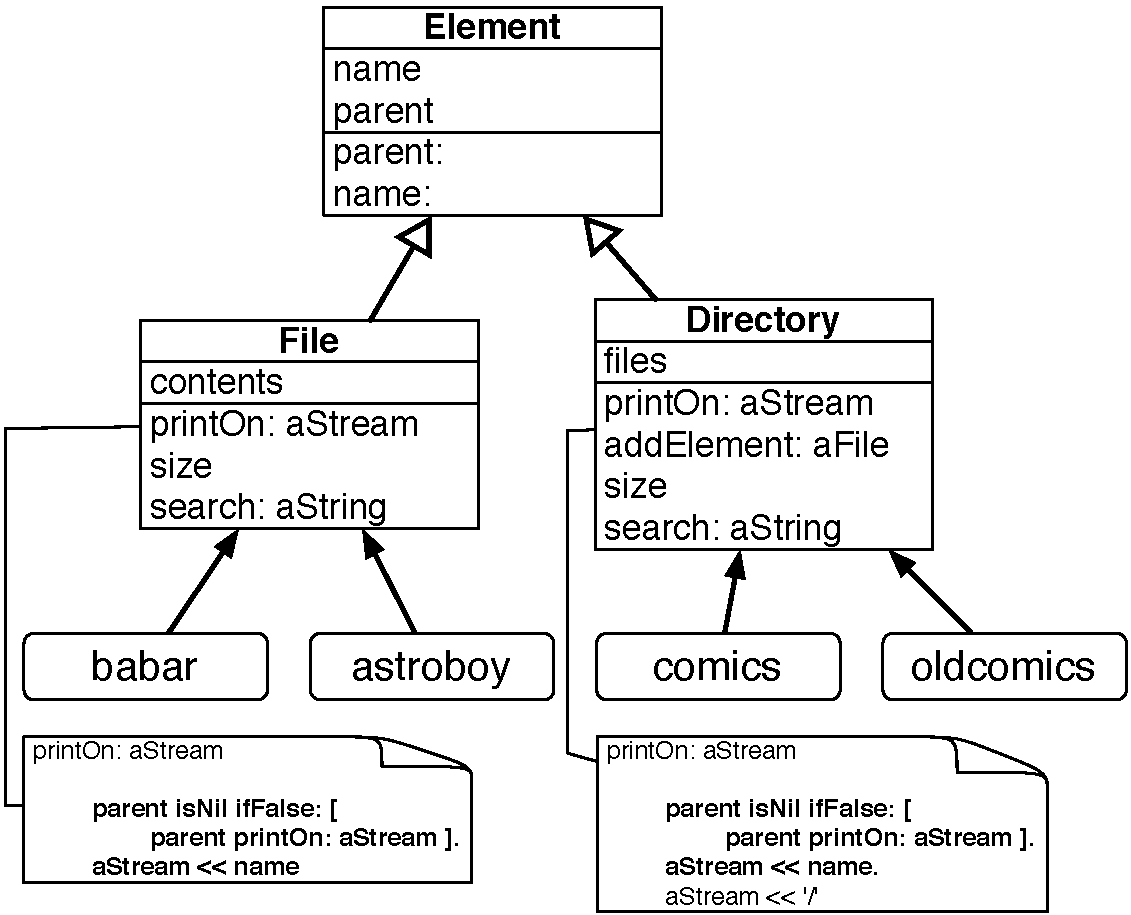
\includegraphics[width=0.65\textwidth]{/Users/ducasse/Workspace/FirstCircle/MyBooks/Bk-Writing/PharoBooks/LearningOOPWithPharoTrans/_result/pdf/Chapters/Inheritance/figures/FileDirectorySuperV0.pdf}\caption{\textcode{MFFile} and \textcode{MFDirectory} contain duplicated logic in \textcode{printOn:}.\label{fig:FileDirectorySuperV0}}\end{center}
\end{figure}


When we look at the following \textcode{printOn:} methods defined in the classes \textcode{MFDirectory} and \textcode{MFFile}
we see that there is code repetition (as shown in Figure \ref{fig:FileDirectorySuperV0}).

Here is the repeated code snippet.

\begin{displaycode}{plain}
parent isNil 
	ifFalse: [ parent printOn: aStream ].
aStream << name
\end{displaycode}

Here is the definition in the two classes: 

\begin{displaycode}{plain}
MFDirectory >> printOn: aStream
	parent isNil 
		ifFalse: [ parent printOn: aStream ].
	aStream << name.
	aStream << '/'
\end{displaycode}

\begin{displaycode}{plain}
MFFile >> printOn: aStream
	parent isNil 
		ifFalse: [ parent printOn: aStream ].
	aStream << name
\end{displaycode}

It means that if we define a new subclass we will have probably duplicate the same expression.
\section{Improving the situation}
To improve the situation above we move up the definition of the \textcode{MFFile} class because it also works for \textcode{MFElement} (as shown in Figure \ref{fig:FileDirectorySuperV1}).

\begin{displaycode}{plain}
MFElement >> printOn: aStream
	parent isNil 
		ifFalse: [ parent printOn: aStream ].
	aStream << name
\end{displaycode}


\begin{figure}

\begin{center}
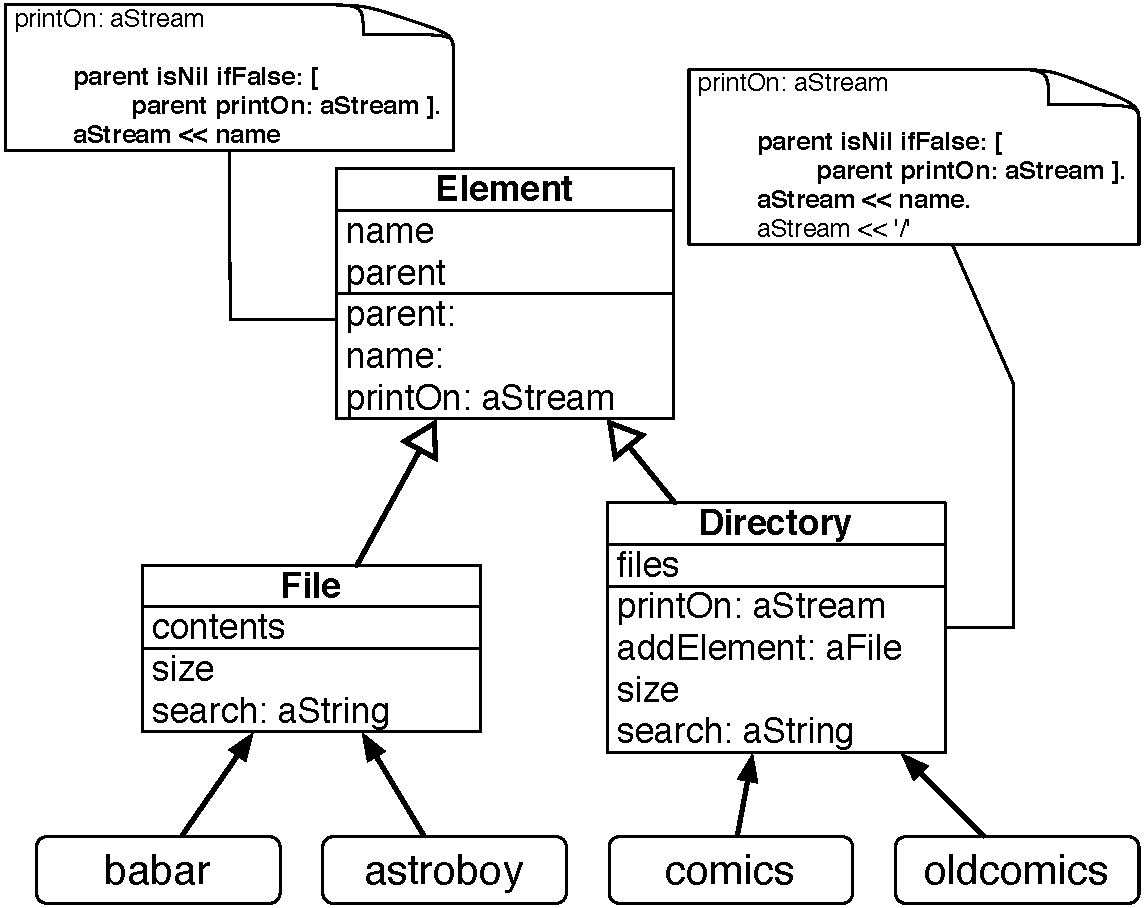
\includegraphics[width=0.65\textwidth]{/Users/ducasse/Workspace/FirstCircle/MyBooks/Bk-Writing/PharoBooks/LearningOOPWithPharoTrans/_result/pdf/Chapters/Inheritance/figures/FileDirectorySuperV1.pdf}\caption{Improving the logic (but not fully).\label{fig:FileDirectorySuperV1}}\end{center}
\end{figure}


\begin{displaycode}{plain}
MFDirectory >> printOn: aStream
	parent isNil 
		ifFalse: [ parent printOn: aStream ].
	aStream << name.
	aStream << '/'
\end{displaycode}

It means that when we will add a new subclass, this class will at least have a default definition for the \textcode{printOn:} method. 

Now the duplication of logic is not addressed. The same code is duplicated between the class \textcode{MFElement} and \textcode{MFDirectory}. What we see is that even if the method \textcode{printOn:} of class \textcode{MFDirectory} is overriding the method of its superclass, we would like to be able to invoke the method of the superclass \textcode{MFElement} and to add the behavior \textcode{aStream \textless{}\textless{} '/'}. 
\subsection{Why self does not work!}
The following definition does not work because it introduces an endless loop. Indeed, since the method lookup starts in the class of the receiver and \textcode{self} represents the receiver, it will always find the same method and will not be able to access the method of the superclass.

\begin{displaycode}{plain}
MFDirectory >> printOn: aStream
	self printOn: aStream.
	aStream << '/'
\end{displaycode}

Let us make sure that you are fully with us. Imagine that we have the following expression: 

\begin{displaycode}{plain}
| p el1 el2 |
p := MFDirectory new name: 'comics'.
el1 := MFFile new name: 'babar'; contents: 'Babar et Celeste'.
p addElement: el1.
el2 := MFFile new name: 'astroboy'; contents: 'super cool robot'.
p addElement: el2.
String streamContents: [:s | p printOn: s ]
\end{displaycode}

\begin{enumerate}
\item We get the message \textcode{p printOn: s}.
\item The method \textcode{printOn:} is looked up starting in the class of \textcode{p}, i.e., \textcode{MFDirectory}.
\item The method is found and applied on \textcode{p}.
\item The message \textcode{self printOn: aStream}  is about to be executed.
\item The receiver is \textcode{self} and represents \textcode{p}. The method \textcode{printOn: aStream} is looked up in the class of the receiver,  i.e., \textcode{MFDirectory}.
\item The same method is found in the class \textcode{MFDirectory} and the process restarts at point 3.
\end{enumerate}

In summary, we would like that while doing an override, to use the behavior we are overriding. This is possible as we will see in the following section. 


\begin{figure}

\begin{center}
\includegraphics[width=0.65\textwidth]{/Users/ducasse/Workspace/FirstCircle/MyBooks/Bk-Writing/PharoBooks/LearningOOPWithPharoTrans/_result/pdf/Chapters/Inheritance/figures/FileDirectorySuperV2.pdf}\caption{Using \textcode{super} to invoke the overridden method \textcode{printOn:}.\label{fig:FileDirectorySuperV2}}\end{center}
\end{figure}

\section{Extending superclass behavior using super}
Let us implement the solution first and discuss it after. We redefine the method \textcode{printOn:} of the class \textcode{MFDirectory} as follows and shown in Figure \ref{fig:FileDirectorySuperV2}.

\begin{displaycode}{plain}
MFDirectory >> printOn: aStream
	super printOn: aStream.
	aStream << '/'
\end{displaycode}

What we see is that the method \textcode{printOn:} does not contain anymore the duplicated expressions with the method \textcode{printOn:} of the superclass (\textcode{MFElement}). Instead by using the special variable \textcode{super} the superclass method is invoked. Let us look at it in detail.

\begin{itemize}
\item The method \textcode{MFDirectory \textgreater{}\textgreater{} printOn:} overrides the method \textcode{MFElement}: it means that during the lookup (activated because the message \textcode{printOn:} has been sent to instances of \textcode{MFDirectory} or future subclasses), the method \textcode{MFElement \textgreater{}\textgreater{} printOn:} cannot be directly found. Indeed when a message is sent to an object, the corresponding method starts in the class of the receiver, therefore the method in \textcode{MFDirectory} is found.
\end{itemize}

\begin{itemize}
\item Using the special variable \textcode{super}, the method lookup is different than with \textcode{self}. When the expression \textcode{super printOn: aStream} is sent, the lookup does not start anymore from the class of the receiver, it starts \textit{from the superclass of the class containing the expression} \textcode{super printOn:}, i.e. \textcode{MFElement}, therefore the method of the superclass is found and executed. 
\end{itemize}

\begin{itemize}
\item Finally, \textcode{super} like \textcode{self} represents the receiver of the messages (for example an instance of the class \textcode{MFDirectory}). Therefore the method is found in the class \textcode{MFDirectory} and executed on the original object that first received the message.
\end{itemize}

Let us make sure that you are fully with us. You can compare with the previous execution simulation.

\begin{displaycode}{plain}
| p el1 el2 |
p := MFDirectory new name: 'comics'.
el1 := MFFile new name: 'babar'; contents: 'Babar et Celeste'.
p addElement: el1.
el2 := MFFile new name: 'astroboy'; contents: 'super cool robot'.
p addElement: el2.
String streamContents: [:s | p printOn: s ]
\end{displaycode}

\begin{enumerate}
\item We get the message \textcode{p printOn: s}.
\item The method \textcode{printOn:} is looked up starting in the class of \textcode{p}, i.e., \textcode{MFDirectory}.
\item The method is found and applied on \textcode{p}.
\item The message \textcode{super printOn: aStream}  is about to be executed.
\item The receiver is \textcode{super} and represents \textcode{p}. The method \textcode{printOn: aStream} is looked up in the superclass of the class containing the expression. The class containing the method is \textcode{MFDirectory}, its superclass is then \textcode{MFElement}. The lookup starts from \textcode{MFElement}.
\item The method is found in the class \textcode{MFElement} in the class.
\item The message \textcode{parent isNil} is treated on the receiver \textcode{p}.
\end{enumerate}

What we see is that using \textcode{super}, the programmer can extend the superclass behavior and reuse by involving it.

\begin{important}
\textcode{super} is the receiver of the message but when we send a message to \textcode{super} the method lookup starts in the superclass of \textbf{the class containing} the expression \textcode{super}.
\end{important}
\section{Another example}
Before explaining with a more theoritical scenario \textit{super} semantics, we want to show another example that illustrates that super expressions do not have to be the first expression of a method. We can invoke the overridden method at any place inside the overriding method.

The example could be more realistic but it shows that super expression does not have to be the first expression of a method.

Let us check the two definitions of the two methods \textcode{size} in \textcode{MFDirectory} and \textcode{MFFile}, we see that \textcode{name size} is used in both.

\begin{displaycode}{plain}
MFDirectory >> size
	| sum |
	sum := 0.
	files do: [ :each | sum := sum + each size ].
	sum := sum + name size.
	sum := sum + 2.
	^ sum
\end{displaycode}

\begin{displaycode}{plain}
MFFile >> size
	^ contents size + name size
\end{displaycode}


\begin{figure}

\begin{center}
\includegraphics[width=0.65\textwidth]{/Users/ducasse/Workspace/FirstCircle/MyBooks/Bk-Writing/PharoBooks/LearningOOPWithPharoTrans/_result/pdf/Chapters/Inheritance/figures/FileDirectorySuperV3.pdf}\caption{Using \textcode{super} to invoke the overridden method \textcode{size}.\label{fig:FileDirectorySuperV3}}\end{center}
\end{figure}


What we can do is the following: define \textcode{size} in the superclass and invoke it using \textcode{super} as shown in Figure \ref{fig:FileDirectorySuperV3}. Here is then the resulting situation.

\begin{displaycode}{plain}
MFElement >> size
	^ name size
\end{displaycode}

\begin{displaycode}{plain}
MFFile >> size
	^ contents size + super size
\end{displaycode}

\begin{displaycode}{plain}
MFDirectory >> size
	| sum |
	sum := 0.
	files do: [ :each | sum := sum + each size ].
	sum := sum + super size.
	sum := sum + 2.
	^ sum
\end{displaycode}

What you see is that messages sent to \textcode{super} can be used anywhere inside in the overriding method and their results can be used as any other messages.
\section{Really understanding super}
To convince you that \textcode{self} and \textcode{super} points to the same object you can use the message \textcode{==} to verify it as follows: 

\begin{displaycode}{plain}
MFFile >> funky
	^ super == self
\end{displaycode}

\begin{displaycode}{plain}
MFFile new funky
>>> true
\end{displaycode}

\begin{important}
\textcode{super} is a special variable: \textcode{super} (just like \textcode{self}) is the receiver of the message! 
\end{important}

Now we take some time to look abstractly at what we presented so far. 
Imagine a situation as illustrated by Figure \ref{fig:LookupWithSuperInSuperclassMethodThreeClasses}.

\begin{displaycode}{plain}
A new bar
>>> ...
C new bar
>>> ...
D new bar
>>> ...
\end{displaycode}
\subsection{Solution }

\begin{figure}

\begin{center}
\includegraphics[width=0.35\textwidth]{/Users/ducasse/Workspace/FirstCircle/MyBooks/Bk-Writing/PharoBooks/LearningOOPWithPharoTrans/_result/pdf/Chapters/Inheritance/figures/LookupWithSuperInSuperclassMethodThreeClasses.pdf}\caption{Example to understand \textcode{super}.\label{fig:LookupWithSuperInSuperclassMethodThreeClasses}}\end{center}
\end{figure}


The solutions are the following ones:

\begin{displaycode}{plain}
A new bar
>>> 10
C new bar
>>> 20
D new bar
>>> 100
\end{displaycode}

Let us examine the evaluation of the message \textcode{aD bar}: 

\begin{enumerate}
\item \textcode{aD}'s class is \textcode{D}.
\item There is no method \textcode{bar} in D.
\item The method look up in \textcode{C}. The method \textcode{bar} is found.
\item The method \textcode{bar} of \textcode{C} is executed.
\item The message \textcode{bar} is sent to \textcode{super}.
\item \textcode{super} represents \textcode{aD} but the lookup starts in the superclass of the class containing the expression \textcode{super} so it starts in \textcode{B}.
\item The method \textcode{bar} is not found in \textcode{B}, the lookup continues in \textcode{A}.
\item The method \textcode{bar} is found in \textcode{A} and it is executed on the receiver i.e., \textcode{aD}.
\item The message \textcode{foo} is sent to \textcode{aD}.
\item The method \textcode{foo} is found in \textcode{D} and executed. It returns 50. 
\item Then to finish the execution of method \textcode{bar} in \textcode{C}, the rest of the expression \textcode{+ self foo} should be executed.
\item Message \textcode{self foo} returns 50 too, so the result returns 100. 
\end{enumerate}

\begin{important}
The difference between \textcode{self} and \textcode{super} is that when we send a message to \textcode{super} the method lookup starts in the superclass of the class containing the expression \textcode{super}.
\end{important}
\section{Conclusion}
In this chapter we saw that inheritance also supports the possibilities to override a method and from this overriding method to invoke the overridden one. This is done using the special variable \textcode{super}. 
\textcode{super} is the receiver of the message like \textcode{self}. The difference is that the method lookup is changed when messages are sent to \textcode{super}. The method is looked up in the superclass of the class containing the message sent to \textcode{super}. 

\chapter{A little expression interpreter}\label{cha:expressions}
In this chapter you will build a small mathematical expression interpreter. For example you will be able to build an expression such as  (3 + 4) * 5 and then ask the interpreter to compute its value. You will revisit tests, classes, messages, methods and inheritance. 
You will also see an example of expression trees similar to the ones that are used to manipulate programs. For example, compilers and code refactorings as offered in Pharo and many modern IDEs are doing such manipulation with trees representing code. 
In addition, in the volume two of this book, we will extend this example to present the Visitor Design Pattern. 
\section{Starting with constant expression and a test}
We start with constant expression. A constant expression is an expression whose value is always the same, obviously.

Let us start by defining a test case class as follows: 

\begin{displaycode}{plain}
TestCase subclass: #EConstantTest
	instanceVariableNames: ''
	classVariableNames: ''
	package: 'Expressions'
\end{displaycode}

 We decided to define one test case class per expression class and this even if at the beginning the classes will not contain many tests. It is easier to define new tests and navigate them.
 
Let us write a first test making sure that when we get a value, sending it the \textcode{evaluate} message returns its value. 

\begin{displaycode}{plain}
EConstantTest >> testEvaluate 
	self assert: (EConstant new value: 5) evaluate equals: 5
\end{displaycode}

When you compile such a test method, the system should prompt you to get a class \textcode{EConstant} defined. 
Let the system drive you. Since we need to store the value of a constant expression, let us add an instance variable \textcode{value}
to the class definition. 

At the end you should have the following definition for the class \textcode{EConstant}.

\begin{displaycode}{plain}
Object subclass: #EConstant
	instanceVariableNames: 'value'
	classVariableNames: ''
	package: 'Expressions'
\end{displaycode}

We define the method \textcode{value:} to set the value of the instance variable \textcode{value}.
It is simply a method taking one argument and storing it in the \textcode{value} instance variable.

\begin{displaycode}{plain}
EConstant >> value: anInteger
	value := anInteger
\end{displaycode}

You should define the method \textcode{evaluate}: it should return the value of the constant. 

\begin{displaycode}{plain}
EConstant >> evaluate
	... Your code ...
\end{displaycode}

Your test should pass. 
\section{Negation}
Now we can start to work on expression negation. Let us write a test and for this define a new test case class named \textcode{ENegationTest}. 

\begin{displaycode}{plain}
TestCase subclass: #ENegationTest
	instanceVariableNames: ''
	classVariableNames: ''
	package: 'Expressions'
\end{displaycode}

The test \textcode{testEvaluate} shows that a negation applies to an expression (here a constant) and when we evalute we get the negated value of the constant. 

\begin{displaycode}{plain}
ENegationTest >> testEvaluate 
	self assert: (ENegation new expression: (EConstant new value: 5)) evaluate equals: -5
\end{displaycode}

Let us execute the test and let the system help us to define the class. A negation defines an instance variable to hold the expression that it negates.

\begin{displaycode}{plain}
Object subclass: #ENegation
	instanceVariableNames: 'expression'
	classVariableNames: ''
	package: 'Expressions'
\end{displaycode}

We define a setter method to be able to set the expression under negation.

\begin{displaycode}{plain}
ENegation >> expression: anExpression 
	expression := anExpression
\end{displaycode}

Now the \textcode{evaluate} method should request the evaluation of the expression and negate it. 
To negate a number the Pharo library proposes the message \textcode{negated}. 

\begin{displaycode}{plain}
ENegation >> evaluate
	... Your code ...
\end{displaycode}


\begin{figure}

\begin{center}
\includegraphics[width=0.7\textwidth]{/Users/ducasse/Workspace/FirstCircle/MyBooks/Bk-Writing/PharoBooks/LearningOOPWithPharoTrans/_result/pdf/Chapters/Expressions/figures/Expressions.png}\caption{A flat collection of classes (with a suspect duplication).\label{figExpression}}\end{center}
\end{figure}


Following the same principle, we will add expression addition and multiplication. Then we will make the system a bit more easy to manipulate and revisit its first design. 
\section{Adding expression addition}
To be able to do more than constant and negation we will add two extra expressions: addition and multiplication and after we will discuss about our approach and see how we can improve it.  

To add an expression that supports addition, we start to define a test case class and a simple test. 

\begin{displaycode}{plain}
TestCase subclass: #EAdditionTest
	instanceVariableNames: ''
	classVariableNames: ''
	package: 'Expressions'
\end{displaycode}

A simple test for addition is to make sure that we add correctly two constants. 

\begin{displaycode}{plain}
EAdditionTest >> testEvaluate
	| ep1 ep2 |
	ep1 := (EConstant new value: 5).
	ep2 := (EConstant new value: 3).
	self assert: (EAddition new right: ep1; left: ep2) evaluate equals: 8
\end{displaycode}

	
You should define the class \textcode{EAddition}: it has two instance variables for the two subexpressions it adds. 

\begin{displaycode}{plain}
EExpression subclass: #EAddition
	instanceVariableNames: 'left right'
	classVariableNames: ''
	package: 'Expressions'
\end{displaycode}

Define the two corresponding setter methods \textcode{right:} and \textcode{left:}. 

Now you can define the \textcode{evaluate} method for addition. 

\begin{displaycode}{plain}
EAddition >> evaluate
	... Your code ...
\end{displaycode}

	
To make sure that our implementation is correct we can also test that we can add negated expressions. 
It is always good to add tests that cover \textit{different} scenario. 
	

\begin{displaycode}{plain}
EAdditionTest >> testEvaluateWithNegation
	| ep1 ep2 |
	ep1 := ENegation new expression: (EConstant new value: 5).
	ep2 := (EConstant new value: 3).
	self assert: (EAddition new right: ep1; left: ep2) evaluate equals: -2
\end{displaycode}

	
	
\section{Multiplication}
We do the same for multiplication: create a test case class named \textcode{EMultiplicationTest}, a test, a new class \textcode{EMultiplication}, a couple of setter methods and finally a new \textcode{evaluate} method. Let us do it fast and without much comments. 

\begin{displaycode}{plain}
TestCase subclass: #EMultiplicationTest
	instanceVariableNames: ''
	classVariableNames: ''
	package: 'Expressions'
\end{displaycode}

\begin{displaycode}{plain}
EMultiplicationTest >> testEvaluate
	| ep1 ep2 |
	ep1 := (EConstant new value: 5).
	ep2 := (EConstant new value: 3).
	self assert: (EMultiplication new right: ep1; left: ep2) evaluate equals: 15
\end{displaycode}

\begin{displaycode}{plain}
Object subclass: #EMultiplication
	instanceVariableNames: 'left right'
	classVariableNames: ''
	package: 'Expressions'
\end{displaycode}

\begin{displaycode}{plain}
EMultiplication >> right: anExpression
	right := anExpression
\end{displaycode}

\begin{displaycode}{plain}
EMultiplication >> left: anExpression
	left := anExpression
\end{displaycode}

\begin{displaycode}{plain}
EMultiplication >> evaluate
	... Your code ...
\end{displaycode}
\section{Stepping back }
It is interesting to look at what we built so far. We have a group of classes whose instances can be combined to create complex expressions. Each expression is in fact a tree of subexpressions as shown in Figure \ref{fig:ExpressionTrees}. The figure shows two main trees: one  for the constant expression \textcode{5} and one for the expression \textcode{-5 + 3}. Note that the diagram represents the number 5 as an object because in Pharo even small integers are objects in the same way the instances of \textcode{EConstant} are objects. 


\begin{figure}

\begin{center}
\includegraphics[width=0.6\textwidth]{/Users/ducasse/Workspace/FirstCircle/MyBooks/Bk-Writing/PharoBooks/LearningOOPWithPharoTrans/_result/pdf/Chapters/Expressions/figures/ExpressionTrees.pdf}\caption{Expressions are composed of trees.\label{fig:ExpressionTrees}}\end{center}
\end{figure}

\subsection{Messages and methods}
The implementation of the \textcode{evaluate} message is worth discussing. What we see is that \textit{different} classes understand the same message but execute different methods as shown in Figure \ref{figExpressionEvaluate}.

\begin{important}
A message represents an intent: it represents \textit{what} should be done. A method represents a specification of \textit{how} something should be executed.
\end{important}

What we see is that sending a message \textcode{evaluate} to an expression is making a choice among the different implementations of the message. This point is central to object-oriented programming. 

\begin{important}
Sending a message is making a choice among all the methods with the same name. 
\end{important}
\subsection{About common superclass}
So far we did not see the need to have an inheritance hierarchy because there is not much to share or reuse. Now adding a common superclass would be useful to convey to the reader of the code or a future extender of the library that such concepts are related and are different variations of expression. 


\begin{figure}

\begin{center}
\includegraphics[width=0.8\textwidth]{/Users/ducasse/Workspace/FirstCircle/MyBooks/Bk-Writing/PharoBooks/LearningOOPWithPharoTrans/_result/pdf/Chapters/Expressions/figures/ExpressionsEvaluate.pdf}\caption{Evaluation: one message and multiple method implementations.\label{figExpressionEvaluate}}\end{center}
\end{figure}

\subsection{Design corner: About addition and multiplication model }
We could have just one class called for example BinaryOperation and it can have an operator and this operator will be either 
the addition or multiplication. This solution can work and as usual having a working program does not mean that its design is any good. 

In particular having a single class would force us to start to write conditional based on the operator as follows

\begin{displaycode}{plain}
BinaryExpression >> evaluate
	operator = #+ 
		ifTrue: [ left evaluate + right evaluate ] 
		ifFalse: [ left evaluate * right evaluate]
\end{displaycode}

There are ways in Pharo to make such code more compact but we do not want to use it at this stage. For the interested reader, look for the message \textcode{perform:} that can execute a method based on its name. 

This is annoying because the execution engine itself is made to select methods for us so we want to avoid to bypass it using explicit condition. In addition when we will add power, division, subtraction we will have to have more cases in our condition making the code less
readable and more fragile. 

As we will see as a general message in this book, sending a message is making a choice between different implementations. 
Now to be able to choose we should have different implementations and this implies having different classes. 

\begin{important}
Classes represent choices whose methods can be selected in reaction to a message. Having many little classes is better than few large ones.
\end{important}

What we could do is to introduce a common superclass between \textcode{EAddition} and \textcode{EMultiplication} but keep the two subclasses. We will probably do it in the future
\section{Negated as a message}
Negating an expression is expressed in a verbose way. We have to create explicitly each time an instance of the class \textcode{ENegation} as shown in the following snippet. 

\begin{displaycode}{plain}
ENegation new expression: (EConstant new value: 5)
\end{displaycode}

We propose to define a message \textcode{negated} on the expressions themselves that will create such instance of \textcode{ENegation}.
With this new message, the previous expression can be reduced too. 

\begin{displaycode}{plain}
(EConstant new value: 5) negated
\end{displaycode}
\subsection{negated message for constants}
Let us write a test to make sure that we capture well what we want to get. 

\begin{displaycode}{plain}
EConstantTest >> testNegated
	self assert: (EConstant new value: 6) negated evaluate equals: -6
\end{displaycode}

And now we can simply implement it as follows: 

\begin{displaycode}{plain}
EConstant >> negated
	^ ENegation new expression: self
\end{displaycode}
\subsection{negated message for negations}
\begin{displaycode}{plain}
ENegationTest >> testNegationNegated
	self assert: (EConstant new value: 6) negated negated evaluate equals: 6
\end{displaycode}

\begin{displaycode}{plain}
ENegation >> negated
	^ ENegation new expression: self
\end{displaycode}

This definition is not the best we can do since in general it is a bad practice to hardcode the class usage inside the class. A better definition would be 

\begin{displaycode}{plain}
ENegation >> negated
	^ self class new expression: self
\end{displaycode}

But for now we keep the first one for the sake of simplicity
\subsection{negated message for additions}
We proceed similarly for additions. 

\begin{displaycode}{plain}
EEAdditionTest >> testNegated
	| ep1 ep2 |
	ep1 := EConstant new value: 5.
	ep2 := EConstant new value: 3.
	self assert: (EAddition new right: ep1; left: ep2) negated evaluate equals: -8
\end{displaycode}

\begin{displaycode}{plain}
EAddition >> negated
	Your code
\end{displaycode}
\subsection{negated message for multiplications}
We proceed similarly for multiplications. 

\begin{displaycode}{plain}
EMultiplicationTest >> testEvaluateNegated
	| ep1 ep2 |
	ep1 := EConstant new value: 5.
	ep2 := EConstant new value: 3.
	self assert: (EMultiplication new right: ep1; left: ep2) negated evaluate equals: -15
\end{displaycode}

\begin{displaycode}{plain}
EMultiplication >> negated
	... Your code ...
\end{displaycode}

Now all your tests should pass. And it is a good moment to save your package. 
\section{Annoying repetition}
Let us step back and look at what we have. We have a working situation but again object-oriented design is to bring the code to a better level. 

Similarly to the situation of the \textcode{evaluate} message and methods we see that the functionality of \textcode{negated} is distributed over 
different classes. Now what is annoying is that we repeat the exact \textit{same} code over and over and this is not good (see Figure \ref{fig:ExpressionsNegatedRepeated}). 
This is not good because if tomorrow we want to change the behavior of negation we will have to change it four times while 
in fact one time should be enough. 


\begin{figure}

\begin{center}
\includegraphics[width=0.7\textwidth]{/Users/ducasse/Workspace/FirstCircle/MyBooks/Bk-Writing/PharoBooks/LearningOOPWithPharoTrans/_result/pdf/Chapters/Expressions/figures/ExpressionsNegatedRepeated.pdf}\caption{Code repetition is a bad smell.\label{fig:ExpressionsNegatedRepeated}}\end{center}
\end{figure}


What are the solutions?

\begin{itemize}
\item We could define another class \textcode{Negator} that would do the job and each current classes would delegate to it. But it does not really solve our problem since we will have to duplicate all the message sends to call \textcode{Negator} instances. 
\item If we  define the method \textcode{negated} in the superclass (\textcode{Object}) we only need one definition and it will work. Indeed, when we send the message \textcode{negated} to an instance of \textcode{EConstant} or \textcode{EAddition} the system will not find it locally but in the superclass \textcode{Object}. So no need to define it four times but only one in class \textcode{Object}. This solution is nice because it reduces the number of  similar definitions of the method \textcode{negated} but it is not good because even if in Pharo we can add methods to the class \textcode{Object} this is not a good practice. \textcode{Object} is a class shared by the entire system so we should take care not to add behavior only making sense for a single application. 
\item The solution is to introduce a new superclass between our classes and the class \textcode{Object}. It will have the same property than the solution with \textcode{Object} but without polluting it (see Figure \ref{figExpressionHierar}). This is what we do in the next section. 
\end{itemize}
\section{Introducing Expression class}

\begin{figure}

\begin{center}
\includegraphics[width=0.7\textwidth]{/Users/ducasse/Workspace/FirstCircle/MyBooks/Bk-Writing/PharoBooks/LearningOOPWithPharoTrans/_result/pdf/Chapters/Expressions/figures/ExpressionsHierarchy.png}\caption{Introducing a common superclass.\label{figExpressionHierar}}\end{center}
\end{figure}


Let us introduce a new class to obtain the situation depicted by Figure \ref{figExpressionHierar}. 
We can simply do it by adding a new class:

\begin{displaycode}{plain}
Object subclass: #EExpression
	instanceVariableNames: ''
	classVariableNames: ''
	package: 'Expressions'
\end{displaycode}

and changing all the previous definitions to inherit from \textcode{EExpression} instead of \textcode{Object}.
For example the class \textcode{EConstant} is then defined as follows. 

\begin{displaycode}{plain}
EExpression subclass: #EConstant
	instanceVariableNames: 'value'
	classVariableNames: ''
	package: 'Expressions'
\end{displaycode}

We can also use for the first transformation the class refactoring \textit{Insert superclass}. Refactorings are code transformations that do not change the behavior of a program. You can find it under the refactorings list when you bring the menu on the classes. 
Now it is only useful for the first changes. 

Once the classes \textcode{EConstant}, \textcode{ENegation}, \textcode{EAddition}, and \textcode{EMultiplication} are subclasses of \textcode{EEXpression}, we should focus on the method \textcode{negated}. Now the method refactoring \textit{Push up} will really help us. 

\begin{itemize}
\item Select the method \textcode{negated} in one of the classes
\item Select the refactoring \textit{Push up}
\end{itemize}

The system will define the method \textcode{negated} in the superclass (\textcode{EExpression}) and remove all the negated methods in the classes. Now we obtain the situation described in Figure \ref{figExpressionHierar}. It is a good moment to run all your tests again. They should all pass. 

Now you could think that we can introduce a new class named ArithmeticExpression as a superclass of \textcode{EAddition} and \textcode{EMultiplication}. Indeed this is something that we could do to factor out common structure and behavior between the two classes. We will do it later because this is basically just a repetition of what we have done.
\section{Class creation messages}
Until now we always sent the message new to a class followed by a setter method as shown below. 

\begin{displaycode}{plain}
EConstant new value: 5
\end{displaycode}

We would like to take the opportunity to show that we can define simple \textbf{class} methods to improve the class instance creation interface. In this example it is simple and the benefits are not that important but we think that this is a nice example. With this in mind the previous example can now be written as follows: 

\begin{displaycode}{plain}
EConstant value: 5
\end{displaycode}

Notice the important difference that in the first case the message is sent to the newly created instance while in the second case it is sent to the class itself. 

To define a class method is the same as to define an instance method (as we did until now). The only difference is that using the code browser you should click on the classSide button to indicate that you are defining a method that should be executed in response
to a message sent to a class itself. 
\subsection{Better instance creation for constants}
Define the following method on the class \textcode{EConstant}. Notice the definition now use \textcode{EConstant class} and not just \textcode{EConstant} to stress that we are defining the class method. 

\begin{displaycode}{plain}
EConstant class >> value: anInteger
	^ self new value: anInteger
\end{displaycode}

Now define a new test to make sure that our method works correctly.

\begin{displaycode}{plain}
EConstantTest >> testCreationWithClassCreationMessage
	self assert: (EConstant value: 5) evaluate equals: 5
\end{displaycode}
\subsection{Better instance creation for  negations}
We do the same for the class \textcode{ENegation}.

\begin{displaycode}{plain}
ENegation class >> expression: anExpression
	... Your code ...
\end{displaycode}

We write of course a new test as follows: 

\begin{displaycode}{plain}
ENegationTest >> testEvaluateWithClassCreationMessage
	self assert: (ENegation expression: (EConstant value: 5)) evaluate equals: -5
\end{displaycode}
\subsection{Better instance creation for  additions}
For the addition we  add a class method named \textcode{left:right:} taking two arguments 

\begin{displaycode}{plain}
EAddition class >> left: anInteger right: anInteger2
	^ self new left: anInteger ; right: anInteger2 
\end{displaycode}

Of course, since we are addicted to tests, we add a new test. 

\begin{displaycode}{plain}
EEAdditionTest >> testEvaluateWithClassCreationMessage
	| ep1 ep2 |
	ep1 := EConstant constant5.
	ep2 := EConstant constant3.
	self assert: (EAddition left: ep1 right: ep2) evaluate equals: 8
\end{displaycode}
\subsection{Better instance creation for  multiplications}
We let you do the same for the multiplication. 

\begin{displaycode}{plain}
EMultiplication class >> left: anExp right: anExp2
	... Your code ...
\end{displaycode}

And another test to check that everything is ok. 

\begin{displaycode}{plain}
EMultiplicationTest >> testEvaluateWithClassCreationMessage
	| ep1 ep2 |
	ep1 := EConstant new value: 5.
	ep2 := EConstant new value: 3.
	self assert: (EMultiplication new left: ep1; right: ep2) evaluate equals: 15
\end{displaycode}

Run your tests! They should all pass. 
\section{Introducing examples as class messages}
As you saw when writing the tests, it is quite annoying to repeat all the time the expressions to get a given tree. This is especially the case in the tests related to addition and multiplication as the one below: 

\begin{displaycode}{plain}
EEAdditionTest >> testNegated
	| ep1 ep2 |
	ep1 := EConstant new value: 5.
	ep2 := EConstant new value: 3.
	self assert: (EAddition new right: ep1; left: ep2) negated evaluate equals: -8
\end{displaycode}

One simple solution is to define some class methods returning typical instances of their classes. To define a class method remember that you should click the class side button. 

\begin{displaycode}{plain}
EConstant class >> constant5
	^ self new value: 5
\end{displaycode}

\begin{displaycode}{plain}
EConstant class >> constant3
	^ self new value: 3
\end{displaycode}

This way we can define the test as follows:

\begin{displaycode}{plain}
EEAdditionTest >> testNegated
	| ep1 ep2 |
	ep1 := EConstant constant5.
	ep2 := EConstant constant3.
	self assert: (EAddition new right: ep1; left: ep2) negated evaluate equals: -8
\end{displaycode}

The tools in Pharo support such a practice. If we tag a class method with the special annotation \textcode{\textless{}sampleInstance\textgreater{}} the browser will show a little icon on the side and when we click on it, it will open an inspector on the new instance. 

\begin{displaycode}{plain}
EConstant class >> constant3
	<sampleInstance>
	^ self new value: 3
\end{displaycode}

using the same idea we defined the following class methods to return some examples of our classes.

\begin{displaycode}{plain}
EAddition class >> fivePlusThree
	<sampleInstance>
	| ep1 ep2 |
	ep1 := EConstant new value: 5.
	ep2 := EConstant new value: 3.
	^ self new left: ep1 ; right: ep2 
\end{displaycode}

\begin{displaycode}{plain}
EMultiplication class >> fiveTimesThree
	<sampleInstance>
	| ep1 ep2 |
	ep1 := EConstant constant5.
	ep2 := EConstant constant3.
   ^ EMultiplication new left: ep1 ; right: ep2 
\end{displaycode}

What is nice with such examples is that 

\begin{itemize}
\item they help documenting the class by providing objects that we can directly use,
\item they support the creation of tests by providing objects that can serve as input for tests,
\item they simplify the writing of tests. 
\end{itemize}

So think to use them. 
\section{Printing}
It is quite annoying that we cannot really see an expression when we inspect it. We would like to get something better than \textcode{'aEConstant'} and \textcode{'anEAddition'} when we debug our programs.
To display such information the debugger and inspector send to the objects the message \textcode{printString} which by default just prefix the name of the class with 'an' or 'a'. 

Let us change this situation. For this, we will specialize the method \textcode{printOn: aStream}. The message \textcode{printOn:} is called on the object when a program or the system send to the object the message \textcode{printString}. From that perspective \textcode{printOn:} is a system customization point that developers can take advantage to enhance their programming experience.

Note that we do not redefine the method \textcode{printString} because it is more complex and \textcode{printString} is reused for all the objects in the system. We just have to implement the part that is specific to a given class. In object-oriented design jargon, \textcode{printString} is a template method in the sense that it sets up a context which is shared by other objects and it hosts hook methods which are program customization points. \textcode{printOn:} is a hook method. The term hook comes from the fact that code of subclasses are invoked in the hook place (see Figure \ref{fig:ExpressionsHierarchyPrintOn}).

The default definition of the method \textcode{printOn:} as defined on the class \textcode{Object} is the following: it grabs the class name and checks if it starts with a vowel or not and write to the stream the 'a/an class'. This is why by default we got \textcode{'anEConstant'} when we printed a constant expression. 

\begin{displaycode}{plain}
Object >> printOn: aStream
	"Append to the argument, aStream, a sequence of characters that  
	identifies the receiver."
	| title |
	title := self class name.
	aStream
		nextPutAll: (title first isVowel ifTrue: ['an '] ifFalse: ['a ']);
		nextPutAll: title
\end{displaycode}


\begin{figure}

\begin{center}
\includegraphics[width=0.7\textwidth]{/Users/ducasse/Workspace/FirstCircle/MyBooks/Bk-Writing/PharoBooks/LearningOOPWithPharoTrans/_result/pdf/Chapters/Expressions/figures/ExpressionsHierarchyPrintOn.pdf}\caption{printOn: and printString a \symbol{34}hooks and template\symbol{34} in action.\label{fig:ExpressionsHierarchyPrintOn}}\end{center}
\end{figure}

\subsection{A word about streams}
A stream is basically a container for a sequence of objects. Once we get a stream we can either read from it or write to it. In our case we will write to the stream. Since the stream passed to printOn: is a stream expecting characters we will add characters or strings (sequence of characters) to it. We will use the messages: \textcode{nextPut: aCharacter} and \textcode{nextPutAll: aString}. 
They add to the stream the arguments at the next position and following. We will guide you and it is simple. 
You can find more information on the chapter about Stream in the book: Pharo by Example available at \url{http://books.pharo.org}
\subsection{Printing constant}
Let us start with a test. Here we check that a constant is printed as its value.

\begin{displaycode}{plain}
EConstantTest >> testPrinting
	self assert: (EConstant value: 5) printString equals: '5'
\end{displaycode}

The implementation is then simple. We just need to put the value converted as a string to the stream.
 

\begin{displaycode}{plain}
EConstant >> printOn: aStream
	aStream nextPutAll: value printString
\end{displaycode}
\subsection{Printing negation}
For a negation we should first put a '-' and then recurvisely call the printing process on the negated expression. Remember that sending the message \textcode{printString} to an expression should return its string representation.  At least until now it will work for constants. 

\begin{displaycode}{plain}
(EConstant value: 6) printString
>>> '6'
\end{displaycode}

Here is a possible definition

\begin{displaycode}{plain}
ENegation >> printOn: aStream
	aStream nextPutAll: '- '
	aStream nextPutAll: expression printString
\end{displaycode}

By the way since all the messages are sent to the same object, this method can be rewritten as:

\begin{displaycode}{plain}
ENegation >> printOn: aStream
	aStream 
		nextPutAll: '- ';
		nextPutAll: expression printString
\end{displaycode}

We can also define it as follows: 

\begin{displaycode}{plain}
ENegation >> printOn: aStream
	aStream nextPutAll: '- '.
	expression printOn: aStream
\end{displaycode}

The difference between the first solution and the alternate implementation is the following:
In the solution using \textcode{printString}, the system creates two streams: one for each invocation of the message \textcode{printString}. One for printing the expression and one for printing the negation. Once the first stream is used the message \textcode{printString} converts the stream contents into a string and this new string is put inside the second stream which at the end is converted again as a string. So the first solution is not really efficient. 
With the second solution, only one stream is created and each of the method just put the needed string elements inside. 
At the end of the process, the single \textcode{printString} message converts it into a string. 
\subsection{Printing addition}
Now let us write yet another test for addition printing. 

\begin{displaycode}{plain}
EAdditionTest >> testPrinting
	self assert: (EAddition fivePlusThree) printString equals:  '( 5 + 3 )'.
	self assert: (EAddition fivePlusThree) negated printString equals:  '- ( 5 + 3 )'
\end{displaycode}

Printing an addition is: put an open parenthesis, print the left expression, put ' + ', print the right expression and put a closing parenthesis in the stream. 

\begin{displaycode}{plain}
EAddition >> printOn: aStream
	... Your code ...
\end{displaycode}
\subsection{Printing multiplication}
And now we do the same for multiplication. 

\begin{displaycode}{plain}
EMultiplicationTest >> testPrinting
	self assert: (EMultiplication fiveTimesThree) negated printString equals:  '- ( 5 * 3 )'
\end{displaycode}

\begin{displaycode}{plain}
EMultiplication >> printOn: aStream
	... Your code ...
\end{displaycode}
\section{Revisiting negated message for Negation}
Now we can go back on negating an expression. Our implementation is not nice even if we can negate any expression and get the correct value. If you look at it carefully negating a negation could be better. 
Printing a negated negation illustrates well the problem: we get two minuses instead of none. 

\begin{displaycode}{plain}
(EConstant value: 11) negated 
>> '- 11'

(EConstant value: 11) negated negated
>> '- - 11'
\end{displaycode}

A solution could be to change the printOn: definition and to check if the expression that is negated is a negation 
and in such case to not emit the minus. Let us say it now, this solution is not nice because we do not want to write code
that depends on explicitly checking if an object is of a given class. Remember we want to send message and let the object do some actions. 

A good solution is to \textit{specialize} the message \textcode{negated} so that when it is sent to a \textit{negation} it does not create a new negation that points to the receiver but instead returns the expression itself, otherwise the method implemented in \textcode{EExpression} will be executed. This way the trees created by a \textcode{negated} message can never have negated negation but the arithmetic values obtained are correct. Let us implement this solution, we just need to implement a different version of the method \textcode{negated} for \textcode{ENegation}. 

Let us write a test! Since evaluating a single expression or a double negated one gives the same results, we need to define a structural test. This is what we do with the expression \textcode{exp negated class = ENegation} below.

\begin{displaycode}{plain}
NegationTest >> testNegatedStructureIsCorrect
	| exp |
	exp := EConstant value: 11.
	self assert: exp negated class = ENegation. 
	self assert: exp negated negated equals: exp.
\end{displaycode}

Now you should be able to implement the \textcode{negated} message on \textcode{ENegation}. 

\begin{displaycode}{plain}
ENegation >> negated
	... Your code ...
\end{displaycode}
\subsection{Understanding method override}
When we send a message to an object, the system looks for the corresponding method in the class of the receiver then if it is not defined there, the lookup continues in the superclass of the previous class. 

By adding a method in the class \textcode{ENegation}, we created the situation shown in Figure \ref{fig:ExpressionsHierarchyOptimized}. We said that the message \textcode{negated} is overridden in \textcode{ENegation} because for instances of \textcode{ENegation} it hides the method defined in the superclass \textcode{EExpression}. 

It works the following:

\begin{itemize}
\item When we send the message \textcode{negated} to a constant, the message is not found in the class \textcode{EConstant} and then it is looked up in the class \textcode{EExpression} and it is found there and applied to the receiver (the instance of \textcode{EConstant}).
\end{itemize}

\begin{itemize}
\item When we send the message \textcode{negated} to a negation, the message is found in the class \textcode{ENegation} and executed on the negation expression. 
\end{itemize}


\begin{figure}

\begin{center}
\includegraphics[width=0.7\textwidth]{/Users/ducasse/Workspace/FirstCircle/MyBooks/Bk-Writing/PharoBooks/LearningOOPWithPharoTrans/_result/pdf/Chapters/Expressions/figures/ExpressionsHierarchyOptimized.png}\caption{The message \textcode{negated} is overridden in the class \textcode{ENegation}.\label{fig:ExpressionsHierarchyOptimized}}\end{center}
\end{figure}

\section{Introducing BinaryExpression class}\label{secBinaryExpression}
Now we will take a moment to improve our first design. We will factor out the behavior of \textcode{EAddition} and \textcode{EMultiplication}. 

\begin{displaycode}{plain}
EExpression subclass: #EBinaryExpression
	instanceVariableNames: ''
	classVariableNames: ''
	package: 'Expressions'
\end{displaycode}

\begin{displaycode}{plain}
EBinaryExpression subclass: #EAddition
	instanceVariableNames: 'left right'
	classVariableNames: ''
	package: 'Expressions'
\end{displaycode}

\begin{displaycode}{plain}
EBinaryExpression subclass: #EMultiplication
	instanceVariableNames: 'left right'
	classVariableNames: ''
	package: 'Expressions'
\end{displaycode}

Now we can use again a refactoring to pull up the instance variables \textcode{left} and \textcode{right}, as well as the methods \textcode{left:} and \textcode{right:}.

Select the class \textcode{EMuplication}, bring the menu and select in the Refactoring menu the instance variables refactoring \textit{Push Up}. Then select the instance variables.

Now you should get the following class definitions, where the instance variables are defined in the new class and removed from the two subclasses. 

\begin{displaycode}{plain}
EExpression subclass: #EBinaryExpression
	instanceVariableNames: 'left right'
	classVariableNames: ''
	package: 'Expressions'
\end{displaycode}

\begin{displaycode}{plain}
EBinaryExpression subclass: #EAddition
	instanceVariableNames: ''
	classVariableNames: ''
	package: 'Expressions'
\end{displaycode}

\begin{displaycode}{plain}
EBinaryExpression subclass: #EMultiplication
	instanceVariableNames: ''
	classVariableNames: ''
	package: 'Expressions'
\end{displaycode}

We should get a situation similar to the one of Figure \ref{figExpressionFactoredState}. All your tests should still pass. 


\begin{figure}

\begin{center}
\includegraphics[width=0.7\textwidth]{/Users/ducasse/Workspace/FirstCircle/MyBooks/Bk-Writing/PharoBooks/LearningOOPWithPharoTrans/_result/pdf/Chapters/Expressions/figures/ExpressionsHierarchyStateFactored.png}\caption{Factoring instance variables.\label{figExpressionFactoredState}}\end{center}
\end{figure}


Now we can move the same way the methods. Select the method \textcode{left:} and apply the refactoring \textit{Pull Up Method}.  Do the same for the method \textcode{right:}. 
\subsection{Creating a template and hook method}
Now we can look at the methods \textcode{printOn:} of additions and multiplications. They are really similar: Just the operator is changing. Now we cannot simply copy one of the definitions because it will not work for the other. But what we can do is to apply the same design point that implemented for \textcode{printString} and \textcode{printOn:}: we can create a template and hooks that will be specialized in the subclasses. 

We will use the method \textcode{printOn:} as a template with a hook redefined in each subclass.

Let define the method \textcode{printOn:} in \textcode{EBinaryExpression} and remove the other ones from the two classes \textcode{EAddition} and \textcode{EMultiplication}. 

\begin{displaycode}{plain}
EBinaryExpression >> printOn: aStream
	aStream nextPutAll: '( '.
	left printOn: aStream. 
	aStream nextPutAll: ' + '.
	right printOn: aStream.
	aStream nextPutAll: ' )'
\end{displaycode}

Then you can do it manually or use the \textit{Extract Method} Refactoring: This refactoring creates a new method from a part of an existing method and sends a message to the new created method: select the ' + ' inside the method pane and bring the menu and select the Extract Method refactoring, and when prompt give the name \textcode{operatorString}. 

Here is the result you should get:  

\begin{displaycode}{plain}
EBinaryExpression >> printOn: aStream
	aStream nextPutAll: '( '.
	left printOn: aStream.
	aStream nextPutAll: self operatorString.
	right printOn: aStream.
	aStream nextPutAll: ' )'
\end{displaycode}

\begin{displaycode}{plain}
EBinaryExpression >> operatorString
	^ ' + '
\end{displaycode}

Now we can just redefine this method in the \textcode{EMultiplication} class to return the adequate string.

\begin{displaycode}{plain}
EMultiplication >> operatorString
	^ ' * '
\end{displaycode}


\begin{figure}

\begin{center}
\includegraphics[width=0.7\textwidth]{/Users/ducasse/Workspace/FirstCircle/MyBooks/Bk-Writing/PharoBooks/LearningOOPWithPharoTrans/_result/pdf/Chapters/Expressions/figures/ExpressionsHierarchyStateBehaviorFactored.png}\caption{Factoring instance variables and behavior.\label{figExpressionsHierarchyStateBehaviorFactored}}\end{center}
\end{figure}

\section{What did we learn}
The introduction of the class \textcode{EBinaryExpression} is a rich experience in terms of lessons that we can learn. 

\begin{itemize}
\item Refactorings are more than simple code transformations. Usually refactorings pay attention that their application does not change the behavior of programs. As we saw refactorings are powerful operations that really help doing complex operations in a few action.
\end{itemize}

\begin{itemize}
\item We saw that the introduction of a new superclass and moving instance variables or method to a superclass does not change the structure or behavior of the subclasses. This is because (1) for the state, the structure of an instance is based on the state of its class and all its superclasses, (2) the lookup starts in the class of the receiver and look in superclasses.
\end{itemize}

\begin{itemize}
\item While the method \textcode{printOn:} is by itself a hook for the method \textcode{printString}, it can also play the role of a template method. The method \textcode{operatorString} reuses the context created by the \textcode{printOn:} method which acts as a template method. In fact each time we do a self send we create a hook method that subclasses can specialize.
\end{itemize}
\section{About hook methods}
When we introduced \textcode{EBinaryExpression} we defined the method \textcode{operatorString} as follows:

\begin{displaycode}{plain}
EBinaryExpression >> operatorString
	^ ' + '
\end{displaycode}

\begin{displaycode}{plain}
EMultiplication >> operatorString
	^ ' * '
\end{displaycode}

And you may wonder if it was worth to create a new method in the superclass and so that such one subclass redefines it. 
\subsection{Creating hooks is always good}
First creating a hook is also a good idea. Because you rarely know how your system will be extended in the future. On this little example, we suggest you to add raising to power, division and this can be done with one class and two methods per new operator. 
\subsection{Avoid not documenting hooks}
Second we could have just defined one method \textcode{operatorString} in each subclass and no method in the superclass \textcode{EBinaryExpression}. It would have worked because \textcode{EBinaryExpression} is not meant to have direct instances. Therefore there is no risk that a \textcode{printOn:} message is sent to one of its instance and cause an error because no method \textcode{operatorString} is found. 

The code would have looked like the following: 

\begin{displaycode}{plain}
EAddition >> operatorString
	^ ' + '
\end{displaycode}

\begin{displaycode}{plain}
EMultiplication >> operatorString
	^ ' * '
\end{displaycode}


\begin{figure}

\begin{center}
\includegraphics[width=0.7\textwidth]{/Users/ducasse/Workspace/FirstCircle/MyBooks/Bk-Writing/PharoBooks/LearningOOPWithPharoTrans/_result/pdf/Chapters/Expressions/figures/ExpressionsHierarchyBinaryAbstract.pdf}\caption{Better design: Declaring an abstract method as a way to document a hook method.\label{figExpressionsHierarchyBinaryAbstract}}\end{center}
\end{figure}


Now such a design is not really good because as potential extenders, developers will have to guess reading the subclass definitions that they should also define a method \textcode{operatorString}. A better solution in that case is to define an \textit{abstract} method in the superclass as follows: 

\begin{displaycode}{plain}
EBinaryExpression >> operatorString
	^ self subclassResponsibility
\end{displaycode}

Using the message \textcode{subclassResponsibility} declares that a method is abstract and does nothing except forcing its redefinition: subclasses should redefine it explicitly. Using such an approach we get the final situation represented in Figure \ref{figExpressionsHierarchyBinaryAbstract}. 

In the solution presented before (section \ref{secBinaryExpression}) we decided to go for the simplest solution and it was to use one of the default value (' + ') as a default definition for the hook in the superclass \textcode{EExpression}.  It was not a good solution and we did it on purpose to be able to have this discussion. It was not a good solution since it was using a specific subclass. It is better to define a default value for a hook in the superclass when this default value makes sense in the class itself.

Note that we could also define \textcode{evaluate} as an abstract method in \textcode{EExpression} to indicate clearly that each subclass should 
define an \textcode{evaluate}.
\section{Variables}
Up until now our mathematical expressions are rather limited. We only manipulate constant-based expressions. What we would like is to be able to manipulate variables too. 
Here is a simple test to show what we mean: we define a variable named \textcode{'x'} and then we can later specify that \textcode{'x'} should take a given value. 

Let us create a new test class named \textcode{EVariableTest} and define a first test \textcode{testValueOfx}.

\begin{displaycode}{plain}
EVariableTest >> testValueOfx
	self assert: ((EVariable new id: #x) evaluateWith: {#x -> 10} asDictionary) equals: 10.
\end{displaycode}
\subsection{Some technical points}
Let us explain a bit what we are doing with the expression \textcode{\{\#x -\textgreater{} 10\} asDictionary}. We should be able to specify that a given variable name is associated with a given value. For this we create a dictionary: a dictionary is a data structure for storing keys and their associated value. Here a key is the variable and the value its associated value. Let us present some details first.
\subsubsection{Dictionaries}
A dictionary is a data structure containing pairs (key value) and we can access the value of a given key. It can use any object as key and any object as values. Here we simply use a symbol \textcode{\#x} since symbols are unique within the system and as such we are sure that we cannot have two keys looking the same but having different values. 

\begin{displaycode}{plain}
| d |
d := Dictionary new
	at: #x put: 33;
	at: #y put: 52;
	at: #z put: 98.
d at: y
>>> 52 
\end{displaycode}

The previous dictionary can be easily expressed more compactly using \textcode{\{\#x -\textgreater{} 33 . \#y -\textgreater{} 52 . \#z -\textgreater{} 98\} asDictionary}.

\begin{displaycode}{plain}
{#x -> 33 . #y -> 52 . #z -> 98} asDictionary at: #y
>>> 52 
\end{displaycode}
\subsubsection{Dynamic Arrays}
The expression \textcode{\{ \}} creates a dynamic array. Dynamic arrays execute their expressions and store the resulting values. 

\begin{displaycode}{plain}
{2 + 3 . 6 - 2 . 7-2 }
>>> #(5 4 5)
\end{displaycode}
\subsubsection{Pairs}
The expression \textcode{\#x -\textgreater{} 10} creates a pair with a key and a value.

\begin{displaycode}{plain}
| p |
p := #x -> 10.
p key 
>>> #x
p value
>>> 10
\end{displaycode}
\subsection{Back to variable expressions}
If we go a step further, we want to be able to build more complex expressions where instead of having constants we can manipulate variables. This way we will be able to build more advanced behavior such as expression derivations. 

\begin{displaycode}{plain}
EExpression subclass: #EVariable
	instanceVariableNames: 'id'
	classVariableNames: ''
	package: 'Expressions'
\end{displaycode}

\begin{displaycode}{plain}
EVariable >> id: aSymbol
	id := aSymbol
\end{displaycode}

\begin{displaycode}{plain}
EVariable >> printOn: aStream
	aStream nexPutAll: id asString
\end{displaycode}

What we see is that we need to be able to pass bindings (a binding is a pair key, value) when evaluating a variable. The value of a variable is the value of the binding whose key is the name of the variable. 

\begin{displaycode}{plain}
EVariable >> evaluateWith: aBindingDictionary
	^ aBindingDictionary at: id
\end{displaycode}

Your tests should all pass at this point. 

For more complex expressions (the ones that interest us) here are two tests. 

\begin{displaycode}{plain}
EVariableTest >> testValueOfxInNegation
	self assert: ((EVariable new id: #x) negated
		evaluateWith: {#x -> 10} asDictionary) equals: -10
\end{displaycode}

What the second test shows is that we can have an expression and given a different set of bindings the value of the expression will differ. 

\begin{displaycode}{plain}
EVariableTest >> testEvaluateXplusY
	| ep1 ep2 add |
	ep1 := EVariable new id: #x.
	ep2 := EVariable new id: #y.
	add := EAddition left: ep1 right: ep2.
	
	self assert: (add evaluateWith: { #x -> 10 . #y -> 2 } asDictionary) equals: 12.
	self assert: (add evaluateWith: { #x -> 10 . #y -> 12 } asDictionary) equals: 22
\end{displaycode}
\subsection{Non working approaches}
A non working solution would be to add the following method to \textcode{EExpression}

\begin{displaycode}{plain}
EEXpression >> evaluateWith: aDictionary
	^ self evaluate
\end{displaycode}

However it does not work for at least the following reasons: 

\begin{itemize}
\item It does not use its argument. It only works for trees composed out exclusively of constant. 
\item When we send a message \textcode{evaluateWith:} to an addition, this message is then turned into an \textcode{evaluate} message sent to its subexpression and such subexpression do not get an \textcode{evaluateWith:} message but an \textcode{evaluate}.
\end{itemize}

Alternatively we could add the binding to the variable itself and only provide an \textcode{evaluate} message as follows: 

\begin{displaycode}{plain}
(EVariable new id: #x) bindings: { #x -> 10 . #y -> 2 } asDictionary
\end{displaycode}

 But it fully defeats the purpose of what a variable is. We should be able to give different values to a variable embedded inside a complex expression.
\subsection{The solution: adding evaluateWith:}
We should transform all the implementations and message sends from \textcode{evaluate} to \textcode{evaluateWith:} Since this is a tedious task we will use the method refactoring \textit{Add Parameter}.
Since a refactoring applies itself on the complete system, we should be a bit cautious because other Pharo classes implement methods named \textcode{evaluate} and we do not want to impact them. 

So here are the steps that we should follow.

\begin{itemize}
\item Select the Expression package
\item Choose Browse Scoped (it brings a browser with only your package)
\item Using this browser, select a method evaluate
\item Select the \textit{Add Parameter} refactoring: type \textcode{evaluateWith:} as method selector and proceed when prompted for a default value \textcode{Dictionary new}. This last expression is needed because the engine will rewrite all the messages \textcode{evaluate} but \textcode{evaluateWith: Dictionary new}.
\item The system is performing many changes. Check that they only touch your classes and accept them all. 
\end{itemize}

A test like the following one: 

\begin{displaycode}{plain}
EConstant >> testEvaluate 
	self assert: (EConstant constant5) evaluate equals: 5
\end{displaycode}

is transformed as follows: 

\begin{displaycode}{plain}
EConstant >> testEvaluate
	self assert: ((EConstant constant5) evaluateWith: Dictionary new) equals: 5
\end{displaycode}

Your tests should nearly all pass except the ones on variables. Why do they fail?
Because the refactoring transformed message sends \textcode{evaluate} but \textcode{evaluateWith: Dictionary new} and this even in methods \textcode{evaluate}. 

\begin{displaycode}{plain}
EAddition >> evaluateWith: anObject
	^ (right evaluateWith: Dictionary new) + (left evaluateWith: Dictionary new)
\end{displaycode}

This method should be transformed as follows: We should pass the binding to the argument of the \textcode{evaluateWith:} recursive calls.

\begin{displaycode}{plain}
EAddition >> evaluateWith: anObject
	^ (right evaluateWith: anObject) + (left evaluateWith: anObject)
\end{displaycode}

Do the same for the multiplications.

\begin{displaycode}{plain}
ENegation >> evaluateWith: anObject
	^ (expression evaluateWith: anObject) negated
\end{displaycode}
\section{Conclusion}
This little exercise was full of learning potential. Here is a little summary of what we explained and we hope you understood. 

\begin{itemize}
\item A message specifies an intent while a method is a named list of execution. We often have one message and a list of methods with the same name. 
\item Sending a message is finding the method corresponding to the message selector: this selection is based on the class of the object receiving the message. When we look for a method we start in the class of the receiver and go up the inheritance link. 
\item Tests are a really nice way to specify what we want to achieve and then to verify after each change that we did not break something. Tests do not prevent bugs but they help us building confidence in the changes we do by identifying fast errors. 
\item Refactorings are more than simple code transformations. Usually refactorings pay attention that their application does not change the behavior of program. As we saw refactorings are powerful operations that really help doing complex operations in a few actions. 
\item We saw that the introduction of a new superclass and moving instance variables or method to a superclass does not change the structure or behavior of the subclasses. This is because (1) for the state, the structure of an instance is based on the state of its class and all its superclasses, (2) the lookup starts in the class of the receiver and look in superclasses. 
\item Each time we send a message, we create a potential place (a hook) for subclasses to get their code definition used in place of the superclass's one.
\end{itemize}

\part{Little projects}
\chapter{A simple network simulator }\label{ch:lan}
In this chapter, we develop a simulator for a computer network, step by step from scratch.
The program starts with a simplistic model of a computer network, made of objects that represent different parts of a local network such as packets, nodes, workstations, routers and hubs.

At first, we will just simulate the different steps of packet delivery and have fun with the system.
In a second step we will extend the basic functionalities by adding extensions such as a hub and different packet routing strategies.
Doing so, we will revisit many object-oriented concepts such as polymorphism, encapsulation, hooks and templates.
Finally this system could be refined to become an experiment platform to explore and understand distributed algorithms.


\begin{figure}

\begin{center}
\includegraphics[width=0.8\textwidth]{/Users/ducasse/Workspace/FirstCircle/MyBooks/Bk-Writing/PharoBooks/LearningOOPWithPharoTrans/_result/pdf/Chapters/SimpleLAN/figures/lan-overview.pdf}\caption{Two little networks composed of nodes and sending packets over links.\label{/Users/ducasse/Workspace/FirstCircle/MyBooks/Bk-Writing/PharoBooks/LearningOOPWithPharoTrans/_result/pdf/Chapters/SimpleLAN/figures/lan-overview.pdf}}\end{center}
\end{figure}

\subsection{Basic definitions and a starting point}
We need to establish the basic model; what does the description above tell us?
A network is a number of interconnected nodes, which exchange data packets.
We will therefore probably need to model the nodes, the connection links, and the packets:

\begin{itemize}
\item Nodes have addresses, can send and receive packets;
\item Links connect two nodes together, and transmit packets between them;
\item A packet transports a payload and has the address of the node to which it should be delivered; if we want nodes to be able to answer (after reception), packets should also have the address of the node which originally sent it.
\end{itemize}
\section{Packets are simple value objects}
Packets seem to be the simplest objects in our model: we need to create them, and ask them about the data they contain, and that's about it.
Once created, a packet object is merely a passive data structure: it will not change its data, knows nothing of the surrounding network, and has no behavior that we can really talk about.

Let's start by defining a test class and a first test sketching what creating and looking at packets would look like:

\begin{displaycode}{smalltalk}
TestCase subclass: #KANetworkEntitiesTest
    instanceVariableNames: ''
    classVariableNames: ''
    category: 'NetworkSimulator-Tests'
\end{displaycode}

\begin{displaycode}{smalltalk}
KANetworkEntitiesTest >> testPacketCreation
    | src dest payload packet |
    src := Object new.
    dest := Object new.
    payload := Object new.

    packet := KANetworkPacket from: src to: dest payload: payload.

    self assert: packet sourceAddress equals: src.
    self assert: packet destinationAddress equals: dest.
    self assert: packet payload equals: payload
\end{displaycode}

By writing this unit test, we described how we think packets should be created, using a \textcode{from:to:payload:} constructor message, and how it should be accessed, using three messages \textcode{sourceAddress}, \textcode{destinationAddress}, and \textcode{payload}.
Since we have not yet decided what addresses and payloads should look like, we just pass arbitrary objects as parameters; all that matters is that when we ask the packet, it returns the correct object back.

Of course, if we now compile and run this test method, it will fail, because the class \textcode{KANetworkPacket} has not been created yet, nor any of the four above messages.
You can either execute and let the system prompt you when needed or we can define the class:

\begin{displaycode}{smalltalk}
Object subclass: #KANetworkPacket
    instanceVariableNames: 'sourceAddress destinationAddress payload'
    classVariableNames: ''
    category: 'NetworkSimulator-Core'
\end{displaycode}

The class-side constructor method creates an instance, which it returns after sending it an initialization message; nothing original as far as constructors go:

\begin{displaycode}{smalltalk}
KANetworkPacket class >> from: sourceAddress to: destinationAddress payload: anObject
    ... Your code ...
\end{displaycode}

That constructor will need to pass the initialization parameters to the new instance.
It's preferable to define a single initialization method that takes all needed parameters at once, since it is only supposed to be called when creating packets and should not be confused with a setter:

\begin{displaycode}{smalltalk}
KANetworkPacket >> initializeSource: source destination: destination payload: anObject
    ... Your code ...
\end{displaycode}

Once a packet is created, all we need to do with it is to obtain its payload, or the addresses of its source or destination nodes.
Define the following getters:

\begin{displaycode}{smalltalk}
KANetworkPacket >> sourceAddress
	... Your code ...
KANetworkPacket >> destinationAddress
	... Your code ...
KANetworkPacket >> payload
	... Your code ...
\end{displaycode}

Now our test should be running and passing.
That's enough for our admittedly simplistic model of packets; we completely ignore the layers of the OSI model, but it could be an interesting exercise to model them more precisely.
\section{Nodes are known by their address}
The first obvious thing we can say about a network node is that if we want to be able to send packets to it, then it should have an address; let's translate that into a test:

\begin{displaycode}{smalltalk}
KANetworkEntitiesTest >> testNodeCreation
    | address node |
    address := Object new.
    node := KANetworkNode withAddress: address.
    self assert: node address equals: address
\end{displaycode}

Like before, to run this test to completion, we will have to define the \textcode{KANetworkNode} class:

\begin{displaycode}{smalltalk}
Object subclass: #KANetworkNode
    instanceVariableNames: 'address'
    classVariableNames: ''
    category: 'NetworkSimulator-Core'
\end{displaycode}

Then a class-side constructor method taking the address of the new node as parameter:

\begin{displaycode}{smalltalk}
KANetworkNode class >> withAddress: aNetworkAddress
    ^ self new
        initializeAddress: aNetworkAddress;
        yourself
\end{displaycode}

The constructor relies on an instance-side initialization method, and the test asserts that the \textcode{address} accessor works; define them:

\begin{displaycode}{smalltalk}
KANetworkNode >> initializeAddress: aNetworkAddress
	... Your code ...
KANetworkNode >> address
	... Your code ...
\end{displaycode}

Again, our simplistic tests should now pass.
\section{Links are one-way connections between nodes}
After nodes and packets, what about looking at links?
In the real world, network cables are bidirectional, but that's because they have wires going both ways.
Here, we're going to keep it simple and define links as simple one-way connections; to make a two-way connection, we will just use two links, one in each direction.

However, creating links that know their source and destination nodes is not sufficient: \textit{nodes} also need to know about their outgoing links, otherwise they cannot send packets. Let us write a test to cover this.

\begin{displaycode}{smalltalk}
KANetworkEntitiesTest >> testNodeLinking
    | node1 node2 link |
    node1 := KANetworkNode withAddress: #address1.
    node2 := KANetworkNode withAddress: #address2.
    link := KANetworkLink from: node1 to: node2.

    link attach.

    self assert: (node1 hasLinkTo: node2)
\end{displaycode}

This test creates two nodes and a link; after telling the link to \textit{attach} itself, we check that it did so: the source node should confirm that it has an outgoing link to the destination node.
Note that the constructor could have registered the link with \textcode{node1}, but we opted for a separate message \textcode{attach} instead, because it's bad form to have a constructor change other objets; this way we can build links between arbitrary nodes and still have control of when the connection really becomes part of the network model.
For symmetry, we could have specified that \textcode{node2} has an incoming link from \textcode{node1}, but that ends up not being necessary, so we leave that out for now.

Again, we need to define the class of links:

\begin{displaycode}{smalltalk}
Object subclass: #KANetworkLink
    instanceVariableNames: 'source destination'
    classVariableNames: ''
    category: 'NetworkSimulator-Core'
\end{displaycode}

A constructor that passes the two required parameters to an instance-side initialization message:

\begin{displaycode}{smalltalk}
KANetworkLink class >> from: sourceNode to: destinationNode
    ^ self new
        initializeFrom: sourceNode to: destinationNode
\end{displaycode}

As well as the initialization method and accessors:

\begin{displaycode}{smalltalk}
KANetworkLink >> initializeFrom: sourceNode to: destinationNode
	... Your code ...
KANetworkLink >> source
	... Your code ...
KANetworkLink >> destination
	... Your code ...
\end{displaycode}

The \textcode{attach} method of a link should not (and cannot) directly modify the source node, so it must delegate to it instead.

\begin{displaycode}{smalltalk}
KANetworkLink >> attach
    source attach: self
\end{displaycode}

This is an example of separation of concerns: the link knows which node has to do what, but only the node itself knows precisely how to do that.
Here, if a node knows about all its outgoing links, it means it has a collection of those, and attaching a link adds it to that collection:

\begin{displaycode}{smalltalk}
KANetworkNode >> attach: anOutgoingLink
    outgoingLinks add: anOutgoingLink
\end{displaycode}

For this method to compile correctly, we will need to extend \textcode{KANetworkNode} with the new instance variable \textcode{outgoingLinks}, and with the corresponding initialization code:

\begin{displaycode}{smalltalk}
KANetworkNode >> initialize
    outgoingLinks := Set new.
\end{displaycode}

And finally the unit test relied on a predicate method to define in \textcode{KANetworkNode}:

\begin{displaycode}{smalltalk}
KANetworkNode >> hasLinkTo: anotherNode
    ... Your code ...
\end{displaycode}

The method \textcode{hasLinkTo:} should verify that there is at least one outgoing links whose destination is the node passed as argument.  We suggest to have a look at the iterator \textcode{anySatisfy:} to express this logic.

Again, all the tests should now pass.


\begin{figure}

\begin{center}
\includegraphics[width=0.8\textwidth]{/Users/ducasse/Workspace/FirstCircle/MyBooks/Bk-Writing/PharoBooks/LearningOOPWithPharoTrans/_result/pdf/Chapters/SimpleLAN/figures/API1.pdf}\caption{Current API of our three main classes.\label{/Users/ducasse/Workspace/FirstCircle/MyBooks/Bk-Writing/PharoBooks/LearningOOPWithPharoTrans/_result/pdf/Chapters/SimpleLAN/figures/API1.pdf}}\end{center}
\end{figure}

\section{Making our objects more understandable}
When programming we often make mistakes and it is important to help developer to address them. Let us put a breakpoint and 
try to understand the objects. 

\begin{displaycode}{smalltalk}
KANetworkEntitiesTest >> testNodeLinking
	| node1 node2 link |
	node1 := KANetworkNode withAddress: #address1.
	node2 := KANetworkNode withAddress: #address2.
	link := KANetworkLink from: node1 to: node2.
	link attach.
	self halt.
	self assert: (node1 hasLinkTo: node2)
\end{displaycode}

Running the test will open a debugger as the one shown in Figure \ref{debugger}. We get object but their textual representation is too generic to really help us. 


\begin{figure}

\begin{center}
\includegraphics[width=1.0\textwidth]{/Users/ducasse/Workspace/FirstCircle/MyBooks/Bk-Writing/PharoBooks/LearningOOPWithPharoTrans/_result/pdf/Chapters/SimpleLAN/figures/debugger.png}\caption{Navigating specific objects having a generic presentation.\label{debugger}}\end{center}
\end{figure}


The method \textcode{printOn:} is responsible to the printing of the object representation. We will then redefine this method for the different objects we have.

\begin{displaycode}{smalltalk}
KANetworkNode >> printOn: aStream
	aStream nextPutAll: 'Node ('.
	aStream nextPutAll: address , ')'
\end{displaycode}

\begin{displaycode}{smalltalk}
KANetworkLink >> printOn: aStream
	aStream nextPutAll: 'Link'.
	source
		ifNotNil: [ aStream
				nextPutAll: ' ';
				nextPutAll: source address ].
	destination
		ifNotNil: [ aStream
				nextPutAll: ' -> ';
				nextPutAll: destination address ]
\end{displaycode}

Now if we rerun the test we obtain a better user experience as shown in Figure \ref{debuggerXP}: we can see the address of a node and the source and destination of a link.


\begin{figure}

\begin{center}
\includegraphics[width=1.0\textwidth]{/Users/ducasse/Workspace/FirstCircle/MyBooks/Bk-Writing/PharoBooks/LearningOOPWithPharoTrans/_result/pdf/Chapters/SimpleLAN/figures/betterDebugerXP.png}\caption{Navigating objects offering a customized presentation.\label{debuggerXP}}\end{center}
\end{figure}

\section{Simulating the steps of packet delivery}
The next big feature is that nodes should be able to send and receive packets, and links to transmit them.

\begin{displaycode}{smalltalk}
KANetworkEntitiesTest >> testSendAndTransmit
    | srcNode destNode link packet |
    srcNode := KANetworkNode withAddress: #src.
    destNode := KANetworkNode withAddress: #dest.
    link := (KANetworkLink from: srcNode to: destNode) attach; yourself.
    packet := KANetworkPacket from: #address to: #dest payload: #payload.

    srcNode send: packet via: link.
    self assert: (link isTransmitting: packet).
    self deny: (destNode hasReceived: packet).

    link transmit: packet.
    self deny: (link isTransmitting: packet).
    self assert: (destNode hasReceived: packet)
\end{displaycode}

We create and setup two nodes, a link between them, and a packet.
Now, to control which packets get delivered in which order, we specify that it happens in separate, controlled steps.
This will allow us to model packet delivery precisely, to simulate latency, out-of-order reception, etc.:

\begin{itemize}
\item First, we tell the node to send the packet using the message \textcode{send:via:}. At that point, the packet should be passed to the link for transmission, but not completely delivered yet.
\item Then, we tell the link to actually transmit the packet along using the message \textcode{transmit:}, and thus the packet should be received by the destination node.
\end{itemize}
\section{Sending a packet}
To send a packet, the node emits it on the link:

\begin{displaycode}{smalltalk}
KANetworkNode >> send: aPacket via: aLink
    aLink emit: aPacket
\end{displaycode}

For the simulation to be realistic, we do not want the packet to be delivered right away; instead, emitting a packet really just stores it in the link, until the user elects this packet to proceed using the \textcode{transmit:} message.
Storing packets requires adding an instance variable to \textcode{KANetworkLink}, as well as specifying how this instance variable should be initialized.

\begin{displaycode}{smalltalk}
Object subclass: #KANetworkLink
    instanceVariableNames: 'source destination packetsToTransmit'
    classVariableNames: ''
    category: 'NetworkSimulator-Core'
\end{displaycode}

\begin{displaycode}{smalltalk}
KANetworkLink >> initialize
    packetsToTransmit := OrderedCollection new
\end{displaycode}

\begin{displaycode}{smalltalk}
KANetworkLink >> emit: aPacket
    "Packets are not transmitted right away, but stored.
    Transmission is explicitly triggered later, by sending #transmit:."
	
    packetsToTransmit add: aPacket
\end{displaycode}

We also add a testing method to check whether a given packet is currently being transmitted by a link:

\begin{displaycode}{smalltalk}
KANetworkLink >> isTransmitting: aPacket
    ... Your code ...
\end{displaycode}
\section{Transmitting across a link}
Transmitting a packet means telling the link's destination node to receive it. Nodes only consume packets addressed to them; fortunately this is what will happen in our test, so we can worry about the alternative case later (\textcode{notYetImplemented} is a special message that we can use in place of code that we will have to write eventually, but prefer to ignore for now).

\begin{displaycode}{smalltalk}
KANetworkNode >> receive: aPacket from: aLink
    aPacket destinationAddress = address
        ifTrue: [
            self consume: aPacket.
            arrivedPackets add: aPacket ]
        ifFalse: [ self notYetImplemented ]
\end{displaycode}

Consuming a packet represents what the node will do with it at the application level; for now let's just define an empty \textcode{consume:} method, as a placeholder:

\begin{displaycode}{smalltalk}
KANetworkNode >> consume: aPacket
    "Default handling is to do nothing."
\end{displaycode}

After consuming the packet, we remember it did arrive; this is mostly for testing and debugging, but someday we might want to simulate packet losses and re-emissions.
Don't forget to declare and initialize the \textcode{arrivedPackets} instance variable, along with its accessor:

\begin{displaycode}{smalltalk}
KANetworkNode >> hasReceived: aPacket
	... Your code ...
\end{displaycode}

Now we can implement the \textcode{transmit:} message. A link can not transmit packets that have not been sent via it, and once transmitted, the packet should not be on the link anymore. We should remove it from the link list of package to be transmitted
and tell the destination to receive it using the message \textcode{receive:from:}.

\begin{displaycode}{smalltalk}
KANetworkLink >> transmit: aPacket
    "Transmit aPacket to the destination node of the receiver link."
    ... Your code ...
\end{displaycode}

At that point all our tests should pass.
Note that the message \textcode{notYetImplemented} is not called, since our tests do not yet require routing.
Figure \ref{Api2} shows that the API of our classes is getting richer than before. 


\begin{figure}

\begin{center}
\includegraphics[width=0.9\textwidth]{/Users/ducasse/Workspace/FirstCircle/MyBooks/Bk-Writing/PharoBooks/LearningOOPWithPharoTrans/_result/pdf/Chapters/SimpleLAN/figures/API2.pdf}\caption{Richer API.\label{Api2}}\end{center}
\end{figure}

\section{The loopback link}
On a real network, when a node wants to send a packet to itself, it does not need any connection to do so.
In real-world networking stacks, loopback routing shortcuts the lower networking layers; however, this is finer detail than we are modeling here.

Still, we want to model the fact that the loopback link is a little special, so each node will store its own loopback link, separately from the outgoing links. We start to define a test. 

\begin{displaycode}{smalltalk}
KANetworkEntitiesTest >> testLoopback
    | node packet |
    node := KANetworkNode withAddress: #address.
    packet := KANetworkPacket from: #address to: #address payload: #payload.

    node send: packet.
    node loopback transmit: packet.

    self assert: (node hasReceived: packet).
    self deny: (node loopback isTransmitting: packet)
\end{displaycode}

The loopback link is implicitely created as part of the node itself.
We also introduce a new \textcode{send:} message, which takes the responsibility of selecting the link to emit the packet.
For triggering packet transmission, we have to use a specific accessor to find the loopback link of the node.

First, we have to add yet another instance variable in nodes:

\begin{displaycode}{smalltalk}
Object subclass: #KANetworkNode
    instanceVariableNames: 'address outgoingLinks loopback arrivedPackets'
    classVariableNames: ''
    category: 'NetworkSimulator-Core'
\end{displaycode}

As with all instance variables, we have to remember to make sure it is correctly initialized; we thus modify \textcode{initialize}:

\begin{displaycode}{smalltalk}
KANetworkNode >> initialize
    ... Your code ...
\end{displaycode}

The accessor has nothing special:

\begin{displaycode}{smalltalk}
KANetworkNode >> loopback
    ^ loopback
\end{displaycode}

And finally we can focus on the \textcode{send:} method and automatic link selection. The method \textcode{send:} should be more generic than the method \textcode{send:via:} and will be one exposed as a public entry point.

This method has to rely on some routing algorithm to identify which links will transmit the packet closer to its destination.
Since some routing algorithms select more than one link, we will implement routing as an \textit{iteration} method, which evaluates the given block for each selected link.

\begin{displaycode}{smalltalk}
KANetworkNode >> send: aPacket
    "Send aPacket, leaving the responsibility of routing to the node."
    self
        linksTowards: aPacket destinationAddress
        do: [ :link | self send: aPacket via: link ]
\end{displaycode}

One of the simplest routing algorithm is \textit{flooding}: just send the packet via every outgoing link.
Obviously, this is a waste of bandwidth, but it works without any knowledge of the network topology beyond the list of outgoing links.

However, there is one case where we know how to route the packet: if the destination address matches the one of the current node, we can select the loopback link.
The logic of \textcode{linksTowards:do:} is then: compare the packet's destination address with the one of the node, if it is the same, we execute the block using the loopback link, else we simply iterate on the outgoing links of the receiver.

\begin{displaycode}{smalltalk}
KANetworkNode >> linksTowards: anAddress do: aBlock
    "Simple flood algorithm: route via all outgoing links.
    However, just loopback if the receiver node is the routing destination."
    ... Your code ...
\end{displaycode}

Now we have the basic model working, and we can try more realistic examples.
\section{Modeling the network itself}
More realistic tests will require non-trivial networks.
We thus need an object that represents the network as a whole, to avoid keeping many nodes and links in individual variables.
We will introduce a new class \textcode{KANetwork}, whose responsibility is to help us build, assemble then find the nodes and links involved in a network.

Let's start by creating another test class, to keep things in order:

\begin{displaycode}{smalltalk}
TestCase subclass: #KANetworkTest
    instanceVariableNames: 'net hub alone'
    classVariableNames: ''
    category: 'NetworkSimulator-Tests'
\end{displaycode}

Since every test needs to rebuild the whole example network from scratch, we specify so in the \textcode{setUp} method:

\begin{displaycode}{smalltalk}
KANetworkTest >> setUp
    self buildNetwork
\end{displaycode}

Before anything else, let's write a test that will pass once we've made progress; we want to access network nodes given only their addresses. Here we check that we get a hub node based on its address: 

\begin{displaycode}{smalltalk}
KANetworkTest >> testNetworkFindsNodesByAddress
    self
        assert: (net nodeAt: hub address ifNone: [ self fail ])
        equals: hub
\end{displaycode}

We will have to implement this \textcode{nodeAt:ifNone:} on our \textcode{KANetwork} class; but first we need to decide how its instances are built.
Let's build network \textcode{net}, with the main part connected in a star shape around a \textcode{hub} node; a pair of nodes \textcode{ping} and \textcode{pong} are part of the network but not connected to \textcode{hub}, and the \textcode{alone} node is just by itself, not even added to the network as shown in Figure \ref{hub}.


\begin{figure}

\begin{center}
\includegraphics[width=0.5\textwidth]{/Users/ducasse/Workspace/FirstCircle/MyBooks/Bk-Writing/PharoBooks/LearningOOPWithPharoTrans/_result/pdf/Chapters/SimpleLAN/figures/lan-star.pdf}\caption{A hub.\label{hub}}\end{center}
\end{figure}


Expanding a network implies adding new connections and possibly new nodes to it.
If the \textcode{net} object understands a \textcode{connect: aNode to: anotherNode} message, you should be able to build nodes and connect them into a network that matches the figure.

\begin{displaycode}{smalltalk}
KANetworkTest >> buildNetwork
	alone := KANetworkNode withAddress: #alone.
	net := KANetwork new.
	hub := KANetworkNode withAddress: #hub.
	#(mac pc1 pc2 prn)
		do: [ :addr | 
			| node |
			node := KANetworkNode withAddress: addr.
			net connect: node to: hub ].
	net connect: (KANetworkNode withAddress: #ping) to: (KANetworkNode withAddress: #pong)
\end{displaycode}

The name of the \textcode{connect:to:} message suggests that establishing the bidirectional links is the responsibility of the \textcode{net} object. It also has to remember enough info so we can inspect the network topology; we can simply store nodes and links in a couple of sets, even though that representation is a little redundant.
Let's define the class with two instance variables:

\begin{displaycode}{smalltalk}
Object subclass: #KANetwork
    instanceVariableNames: 'nodes links'
    classVariableNames: ''
    category: 'NetworkSimulator-Core'
\end{displaycode}

Whenever we define an instance variable, initialization comes next:

\begin{displaycode}{smalltalk}
KANetwork >> initialize
    ... Your code ...
\end{displaycode}

Now we can give the network the possibility to create links.  This method we will use to add links to the network link collection.

\begin{displaycode}{plain}
KANetwork >> makeLinkFrom: aNode to: anotherNode
	^ KANetworkLink from: aNode to: anotherNode
\end{displaycode}

We add a low level method \textcode{add:} to add a node in a network. 

\begin{displaycode}{smalltalk}
KANetwork >> add: aNode
	nodes add: aNode
\end{displaycode}

To be able to test the network construction we add a little test message;

\begin{displaycode}{smalltalk}
KANetwork >> doesRecordNode: aNode
	^ nodes includes: aNode
\end{displaycode}

Now, we can add isolated nodes to the network, even if it does not seem very useful.
\subsection{Connecting nodes.}
Connecting nodes without ensuring that they are part of the network really does not make sense.
Therefore, when connecting nodes, we will first ensure the nodes are added (by simply adding them in the node Set of the network), then we create and attach links in \textit{both} directions; finally we store both links.

Here is a test covering this aspect.

\begin{displaycode}{plain}
KANetworkTest >> testConnect
	| netw hubb mac pc1 |
	netw := KANetwork new.
	hubb := KANetworkNode withAddress: #hub.
	mac := KANetworkNode withAddress: #mac.
	pc1 := KANetworkNode withAddress: #pc1.

	netw connect: hubb to: mac.
	self assert: (hubb hasLinkTo: mac).
	self assert: (mac hasLinkTo: hubb).
	self assert: (netw doesRecordNode: hubb).
	self assert: (netw doesRecordNode: mac).

	netw connect: hubb to: pc1.
	self assert: (hubb hasLinkTo: pc1).
	self assert: (mac hasLinkTo: hubb)
\end{displaycode}

Now implement the \textcode{connect:to:} method; for concision, note that the \textcode{attach} method we defined previously effectively returns the link.

\begin{displaycode}{smalltalk}
KANetwork >> connect: aNode to: anotherNode
    ... Your code ...
\end{displaycode}

The test \textcode{testConnect} should be green.
\section{Looking up nodes}
At this point, the test \textcode{testNetworkFindsNodesByAddress} should run through \textcode{setUp} but fail in the unit test itself, because we still need to implement node lookup. The base lookup should find the first node that has the requested address, or evaluate a fall-back block (a perfect case for the \textcode{detect:ifNone:} message):

\begin{displaycode}{smalltalk}
KANetwork >> nodeAt: anAddress ifNone: noneBlock
    ... Your code ...
\end{displaycode}

We can also make a convenience \textcode{nodeAt:} method for node lookup, that will raise the predefined \textcode{NotFound} exception if it does not find the node.
Let's first write a test which validates this behavior:

\begin{displaycode}{smalltalk}
KANetworkTest >> testNetworkOnlyFindsAddedNodes
    self
        should: [ net nodeAt: alone address ]
        raise: NotFound
\end{displaycode}

Then we can simply express \textcode{nodeAt:} by delegating to \textcode{nodeAt:ifNone:}.
Note that raise an exception, you simply send the message \textcode{signal} to the exception class. Here we use
the specific class method \textcode{signalFor:in:} defined on the \textcode{NotFound} class.

\begin{displaycode}{smalltalk}
KANetwork >> nodeAt: anAddress
    ^ self
        nodeAt: anAddress
        ifNone: [ NotFound signalFor: anAddress in: self ]
\end{displaycode}
\section{Looking up links}
Next, we want to be able to lookup links between two nodes.
Again we define a new test:

\begin{displaycode}{smalltalk}
KANetworkTest >> testNetworkFindsLinks
    | link |
    self
        shouldnt: [ link := net linkFrom: #pong to: #ping ]
        raise: NotFound.
    self
        assert: link source
        equals: (net nodeAt: #pong).
    self
        assert: link destination
        equals: (net nodeAt: #ping)
\end{displaycode}

And we define the method \textcode{linkFrom:to:} returning the link between source and destination nodes with matching addresses, and signalling \textcode{NotFound} if no such link is found:

\begin{displaycode}{smalltalk}
KANetwork >> linkFrom: sourceAddress to: destinationAddress
    ... Your code ...
\end{displaycode}
\subsection{Final check. }
As a final check, let's try some of the previous tests, first on the isolated \textcode{alone} node, showing that loopback works even without a network connection:

\begin{displaycode}{smalltalk}
KANetworkTest >> testSelfSend
    | packet |
    packet := KANetworkPacket
        from: alone address
        to: alone address
        payload: #something.
    self assert: (packet isAddressedTo: alone).
    self assert: (packet isOriginatingFrom: alone).

    alone send: packet.
    self deny: (alone hasReceived: packet).
    self assert: (alone loopback isTransmitting: packet).

    alone loopback transmit: packet.
    self deny: (alone loopback isTransmitting: packet).
    self assert: (alone hasReceived: packet)
\end{displaycode}

You can see that we used new convenience testing methods \textcode{isAddressedTo:} and \textcode{isOriginatingFrom:} which help inspect the state of a simulated network without explicitly comparing addresses.
However, those methods should not take part in network simulation code, since in the real world nodes can never know their peers other than through their addresses.

\begin{displaycode}{smalltalk}
KANetworkPacket >> isAddressedTo: aNode
    ^ destinationAddress = aNode address
\end{displaycode}

\begin{displaycode}{smalltalk}
KANetworkPacket >> isOriginatingFrom: aNode
    ^ sourceAddress = aNode address
\end{displaycode}

The second test attempts transmitting a packet in the network, between the directly connected nodes \textcode{ping} and \textcode{pong}:

\begin{displaycode}{smalltalk}
KANetworkTest >> testDirectSend
    | packet ping pong link |
    packet := KANetworkPacket from: #ping to: #pong payload: #ball.
    ping := net nodeAt: #ping.
    pong := net nodeAt: #pong.
    link := net linkFrom: #ping to: #pong.

    ping send: packet.
    self assert: (link isTransmitting: packet).
    self deny: (pong hasReceived: packet).

    link transmit: packet.
    self deny: (link isTransmitting: packet).
    self assert: (pong hasReceived: packet)
\end{displaycode}

Both tests should pass with no additional work, since they just reproduce what we already tested in \textcode{KANetworkEntitiesTest} and adding \textcode{KANetwork} did not impact the established behavior of nodes, links, and packets.
\section{Packet delivery with forwarding}
Until now, we only tested packet delivery between directly connected nodes; let's try sending a node so that the packet has to be forwarded through the hub.

\begin{displaycode}{smalltalk}
KANetworkTest >> testSendViaHub
    | hello mac pc1 firstLink secondLink |
    hello := KANetworkPacket from: #mac to: #pc1 payload: 'Hello!'.
    mac := net nodeAt: #mac.
    pc1 := net nodeAt: #pc1.
    firstLink := net linkFrom: #mac to: #hub.
    secondLink := net linkFrom: #hub to: #pc1.

    self assert: (hello isAddressedTo: pc1).
    self assert: (hello isOriginatingFrom: mac).

    mac send: hello.
    self deny: (pc1 hasReceived: hello).
    self assert: (firstLink isTransmitting: hello).

    firstLink transmit: hello.
    self deny: (pc1 hasReceived: hello).
    self assert: (secondLink isTransmitting: hello).

    secondLink transmit: hello.
    self assert: (pc1 hasReceived: hello).
\end{displaycode}

If you run this test, you will see that it fails because of the \textcode{notYetImplemented} message we left earlier in \textcode{receive:from:}; it's time to fix that!
When a node receives a packet but is not the recipient, it should forward the packet:

\begin{displaycode}{smalltalk}
KANetworkNode >> receive: aPacket from: aLink
    aPacket destinationAddress = address
        ifTrue: [
            self consume: aPacket.
            arrivedPackets add: aPacket ]
        ifFalse: [ self forward: aPacket from: aLink ]
\end{displaycode}

Now we need to implement packet forwarding, but there is a trap.
An easy solution would be to simply \textcode{send:} the packet again: the hub would send the packet to all its connected nodes, one of which happens to be \textcode{pc1}, the recipient, so all is good!

\textit{Wrong…}

The packet would be also sent to other nodes than the recipient; what would those nodes do when they receive a packet not addressed to them? Forward it. Where? To all their neighbours, which would forward it again... so when would the forwarding stop?

To fix this, we need hubs to behave differently from nodes.
In reality, hubs work at the lower layers of the OSI model, but our simplified model does not have that level of detail.
We can approximate this by saying that upon reception of a packet addressed to another node, a hub should forward the packet, but a normal node should just ignore it.

Let's first define an empty \textcode{forward:from:} method for nodes, then add a new class for hubs, which will be modeled as nodes with an actual implementation of forwarding:

\begin{displaycode}{smalltalk}
KANetworkNode >> forward: aPacket from: arrivalLink
    "Do nothing. Normal nodes do not route packets."
\end{displaycode}
\section{Introducing a new kind of node}
Now we define the class \textcode{KANetworkHub} that will be the recipient of hub specific behavior. 

\begin{displaycode}{smalltalk}
KANetworkNode subclass: #KANetworkHub
    instanceVariableNames: ''
    classVariableNames: ''
    category: 'NetworkSimulator'
\end{displaycode}

A hub does not have routing information, so all it can do is flood routing, with a catch: the packet must not be sent back from where it arrived, because if that happens to be another hub the packet would bounce back and forth indefinitely. We suggest to take advantage of the message \textcode{linksTowards:do:} that performs an action for all given links to one address.

\begin{displaycode}{smalltalk}
KANetworkHub >> forward: aPacket from: arrivalLink
   ... Your code ...
\end{displaycode}

Now we can use a proper hub in our test, replacing the relevant line in \textcode{KANetworkTest \textgreater{}\textgreater{} buildNetwork}, and check that the \textcode{testSendViaHub} unit test passes.

\begin{displaycode}{smalltalk}
    hub := KANetworkHub withAddress: #hub.
\end{displaycode}

You have now a nice basis for network simulation. In the following we will present some possible extensions. 
\section{Other examples of specialized nodes}
In this section we will present some extensions of the core to support different scenarios. We will propose some tasks to make sure that the extensions are fully working. In addition in this section we do not define tests and we strongly encourage you to start to write tests. At the moment of the book you should be ready to write your own tests and see their values to improve your development process. So take this opportunity to practice.
\subsection{Workstations counting received packets}
We would like to know how many packets specific nodes are receiving. 
In particular when a workstation consumes a packet, it simply increments a packet counter.

Let's start by subclassing \textcode{KANetworkNode}:

\begin{displaycode}{smalltalk}
KANetworkNode subclass: #KANetworkWorkstation
    instanceVariableNames: 'receivedCount'
    classVariableNames: ''
    category: 'NetworkSimulator-Nodes'
\end{displaycode}

We need to initialize the \textcode{receivedCount} instance variable.
Properly redefining \textcode{initialize} is enough, because the address is initialized separately in the constructor method \textcode{KANetworkNode \textgreater{}\textgreater{} withAddress:}; however, it's really important not to forget the \textcode{super initialize} message, because that method does initialize the default node behavior.

\begin{displaycode}{smalltalk}
KANetworkWorkstation >> initialize
    super initialize.
    receivedCount := 0
\end{displaycode}

Now we can redefine \textcode{consume:} accordingly:

\begin{displaycode}{smalltalk}
KANetworkWorkstation >> consume: aPacket
    receivedCount := receivedCount + 1
\end{displaycode}

Define accessors and the \textcode{printOn:} method for debugging. 
Define a test for the behavior of workstation nodes.
\subsection{Printers accumulating printouts}
When a printer consumes a packet, it prints it; we can model the output tray as a list where packet payloads get queued, and the supply tray as the number of blank sheets it contains.

The implementation is very similar; we subclass \textcode{KANetworkNode} to redefine the \textcode{consume:} method:

\begin{displaycode}{smalltalk}
KANetworkNode subclass: #KANetworkPrinter
    instanceVariableNames: 'supply tray'
    classVariableNames: ''
    category: 'NetworkSimulator-Nodes'
\end{displaycode}

\begin{displaycode}{smalltalk}
KANetworkPrinter >> consume: aPacket
    supply > 0 ifTrue: [ ^ self "no paper, do nothing" ].

    supply := supply - 1.
    tray add: aPacket payload
\end{displaycode}

Initialization is a bit different, though; since the standard \textcode{initialize} method has no argument, the only sensible initial value for the \textcode{supply} instance variable is zero:

\begin{displaycode}{smalltalk}
KANetworkPrinter >> initialize
    super initialize.
    supply := 0.
    tray := OrderedCollection new
\end{displaycode}

We therefore need a way to pass the initial supply of paper available to a fresh instance:

\begin{displaycode}{smalltalk}
KANetworkPrinter >> resupply: paperSheets
    supply := supply + paperSheets
\end{displaycode}

For convenience, we can provide an extended constructor to create printers with a non-empty supply in one message:

\begin{displaycode}{smalltalk}
KANetworkPrinter class >> withAddress: anAddress initialSupply: paperSheets
    ^ (self withAddress: anAddress)
        resupply: paperSheets;
        yourself
\end{displaycode}

Define accessors and the \textcode{printOn:} method for debugging purpose. 
Define some test methods for the behavior of printer nodes.
\subsection{Servers answering requests}
When a server node consumes a packet, it converts the payload to uppercase, then sends that back to the sender of the request.

This is yet another subclass which redefines the \textcode{consume:} method, but this time the node is stateless, so we have no initialization or accessor methods to write:

\begin{displaycode}{smalltalk}
KANetworkNode subclass: #KANetworkServer
    instanceVariableNames: ''
    classVariableNames: ''
    category: 'NetworkSimulator-Nodes'
\end{displaycode}

\begin{displaycode}{smalltalk}
KANetworkServer >> consume: aPacket
    | response |
    response := aPacket payload asUppercase.
    self send: (KANetworkPacket
        from: self address
        to: aPacket sourceAddress
        payload: response)
\end{displaycode}

Define a test for the behavior of server nodes.
\section{Conclusion}
In this chapter, we built a little network simulation system, step by step.
We showed the benefit of good protocol decompositions.

As a further extension, we suggest modeling a more realistic network with cycles, as shown in Figure \ref{routing}.
Making this work properly will require replacing hubs with routers and flood routing with more realistic routing algorithms.


\begin{figure}

\begin{center}
\includegraphics[width=0.5\textwidth]{/Users/ducasse/Workspace/FirstCircle/MyBooks/Bk-Writing/PharoBooks/LearningOOPWithPharoTrans/_result/pdf/Chapters/SimpleLAN/figures/lan-routes.pdf}\caption{A possible extension: a more realistic network with a cycle between three router nodes. \label{routing}}\end{center}
\end{figure}


Here is a possible setup for a new family of tests. 

\begin{displaycode}{smalltalk}
KARoutingNetworkTest >> buildNetwork
    | routers |
    net := KANetwork new.

    routers := #(A B C) collect:
        [ :each | KANetworkHub withAddress: each ].
    net connect: routers first to: routers second.
    net connect: routers second to: routers third.
    net connect: routers third to: routers first.

    #(a1 a2) do: [ :addr |
        net connect: routers first
            to: (KANetworkNode withAddress: addr) ].
    #(b1 b2 b3) do: [ :addr |
        net connect: routers second
            to: (KANetworkNode withAddress: addr) ].
    net connect: routers third
        to: (KANetworkNode withAddress: #c1)
\end{displaycode}

\chapter{Snakes and ladders}\label{cha:snakes}
Snakes and Ladders is a simple game suitable for teaching children how to apply rules (\url{http://en.wikipedia.org/wiki/Snakes_and_ladders}). It is dull for adults because there is absolutely no strategy involved, but this makes it easy to implement! 
In this chapter you will implement SnakesAndLadders and we use it as a pretext to explore design questions.


\begin{figure}

\begin{center}
\includegraphics[width=0.7\textwidth]{/Users/ducasse/Workspace/FirstCircle/MyBooks/Bk-Writing/PharoBooks/LearningOOPWithPharoTrans/_result/pdf/Chapters/SnakesAndLadders/figures/snakesAndLadders.png}\caption{An example Snakes and Ladders board with two ladders and a snake.\label{fig:snakes}}\end{center}
\end{figure}

\section{Game rules}
Snakes and Ladders originated in India as part of a family of die games. The game was introduced in England as \symbol{34}Snakes and Ladders\symbol{34} (see Figure \ref{fig:snakes}), then the basic concept was introduced in the United States as \textit{Chutes and Ladders}.
Here is a brief description of the rules: 

\begin{itemize}
\item \textbf{Players:} Snakes and Ladders is played by two to four players, each with her/his own token to move around the board.
\item \textbf{Moving Player}: a player rolls a die, then moves the designated number of tiles, between one and six. Once he lands on a tile, she/he has to perform any action designated by the tile. (Since the rules are fuzzy we decided that we can have multiple players in the same tile).
\item \textbf{Ladders:} If the tile a player lands on is at the bottom of a ladder, she/he should climb the ladder, which brings him to a tile higher on the board.
\item \textbf{Snakes:} If the tile a player lands on is  a head snake, she/he must slide down the snake, landing on a tile closer to the beginning.
\item \textbf{Winning:} the winner is the player who gets to the last tile first, whether by landing on it from a roll, or by reaching it with a ladder. We  decided that when the player does not move if he does not land directly on the last tile, it does not move.
\end{itemize}
\section{Game possible run}
The code snippet below is a possible way to program this game. We take as a board configuration the one depicted in Figure \ref{fig:snakes}. It defines a board game composed of 12 tiles with two ladders and one snake. We  add two players and then start the game.

\begin{displaycode}{plain}
| jill jack game |
game := SLGame new tileNumber: 12.
game 
	setLadderFrom: 2 to: 6;
	setLadderFrom: 7 to: 9;
	setSnakeFrom: 11 to: 5.
game 
	addPlayer: (SLPlayer new name: 'Jill');
	addPlayer: (SLPlayer new name: 'Jack'). 
game play
\end{displaycode}

Since we want to focus on the game logic, you will develop a textual version of the game and avoid any lengthy user interface descriptions.

The following is an example game execution: Two players are on the first tile. The board contains two ladders, {[}2-\textgreater{}6{]} and {[}7-\textgreater{}9{]}, and one snake {[}5\textless{}-11{]}.

Jill rolls a die and throws a 3 and moves to the corresponding tile.
Jack rolls a die and throws a 6 and moves to the corresponding tile and follow its effect, climbing the ladder at tile 7 up to tile 9.
Jack and Jill continue to alternate taking turns until Jill ends up on the last tile.

\begin{displaycode}{plain}
[1<Jill><Jack>][2->6][3][4][5][6][7->9][8][9][10][5<-11][12]
<Jill>throws 3: [1<Jack>][2->6][3][4<Jill>][5][6][7->9][8][9][10][5<-11][12]
<Jack>throws 6: [1][2->6][3][4<Jill>][5][6][7->9][8][9<Jack>][10][5<-11][12]
<Jill>throws 5: [1][2->6][3][4][5][6][7->9][8][9<Jack><Jill>][10][5<-11][12]
<Jack>throws 1: [1][2->6][3][4][5][6][7->9][8][9<Jill>][10<Jack>][5<-11][12]
<Jill>throws 3: [1][2->6][3][4][5][6][7->9][8][9][10<Jack>][5<-11][12<Jill>]
\end{displaycode}
\section{Potential objects and responsibilities}
Take a piece of paper, study the game rules and list any potential objects and their behavior. This is an important exercise to practice, training yourself to discover potential objects and classes.

Techniques such as \textit{Responsibility Driven Design} exist to help programmers during this phase of object discovery. Responsibility Driven Design suggests analysing the documents describing a project, and turning the subjects of sentences into candidate objects and grouping verbs as the behavior of these objects. 
Any synonyms are identifed and used to reduce and gather together similar objects or behavior. 
Then later objects are grouped into classes. Some alternate approaches look for relationship patterns between objects such as part-whole, locations, entity-owner... This could be the topic of a full book.

Here we follow another path:  sketching scenarios. We describe several scenarios and from such scenario we identify key playing objects.

\begin{itemize}
\item Scenario 1. The game is created with a number of tiles. The game must have an end and start tiles. Ladders and snakes should be declared.
\item Scenario 2. Players are declared. They start on the first tiles. 
\item Scenario 3. When player rolls a die, he should move the number of tiles given by the die.
\item Scenario 4. After moving the first player a given number of tiles based on the result of die roll, this is the turn of the second player.
\item Scenario 5. When a player arrives to a ladder start, it should be moved to the ladder end.
\item Scenario 6. When a player should move further than the end tile, he does not move.
\item Scenario 7. When a player ends its course on the end tile, he wins and the game is finished.
\end{itemize}

Such scenarios are interesting because they are a good basis for tests.
\subsection{Possible class candidates}
When reading the rules and the scenario, here is a list of possible classes that we could use.
We will refine it later and remove double or overlapping concepts.

\begin{itemize}
\item Game: keeps track of the game state, the players, and whose turn it is.
\item Board: keeps the tile configuration. 
\item Player:  keeps track of location on the board and moving over tiles.
\item Tile: keeps track of any player on it. 
\item Snake: is a special tile which sends a player back to an earlier tile.
\item Ladder: is a special tile which sends a player ahead to a later tile.
\item First Tile: holds multiple players at the beginning of the game.
\item Last Tile: players must land exactly on this tile, or else they do not move.
\item Die: rolls and indicates the number of tiles that a player must move over.
\end{itemize}

It is not clear if all the objects we identify by looking at the problem and its scenario should be really turned into real objects. Also sometimes it is useful to get more classes to capture behavior and state variations. We should look to have an exact mapping between concepts identified in the problem scenario or description and the implementation. 

From analysing this list we can draw some observations: 

\begin{itemize}
\item Game and Board are probably the same concept and we can merge them.
\item Die may be overkill. Having a full object just to produce a random number may not be worth, especially since we do not have a super fancy user interface showing the die rolling and other effect. 
\item Tile, Snake, Ladder, Last and First Tile all look like tiles with some variations or specific actions. We suspect that we can reuse some logic by creating an inheritance hierarchy around the concept of Tile. 
\end{itemize}
\subsection{About representation }
We can implement the same system using different implementation choices. For example we could have only one class implementing all the game logic and it would work. Some people may also 
argue that this is not a bad solution.

Object-oriented design favors the distribution of the state of the system to different objects.
It is often better to have objects with clear responsibilities. Why? Because you should consider that you will have to rethink, modify or extend your system. We should be able to understand and extend easily a system to be able to reply to new requirements.

Not having a nice object-oriented decomposition for a simple game may not be a problem, as soon as you will start to  model a more complex system not having a good decomposition will hurt you. Real life applications often have a lifetime up to 25 years. 

In addition, imagine that we are a game designer and we want to experiment with different variations and tiles with new properties such as one super special tile changing other tiles, adding snakes before the current player to slow other participants.
\section{About object-oriented design}
When designing a system, you will often have questions that cannot be blindly and automatically answered. Often there is no definite answer. This is what is difficult with object-oriented design and this is why practicing is important. 

What composes the state of an object?
The state of object should characterize the object over its lifetime. For example the name of  player identifies the player.

Now it may happen that some objects just because they are instances of different classes
do not need the same state but still offer the same set of messages. For example the tiles and the ladder/snake tiles have probably a similar API but snake and ladder should hold information of their target tile.

We can also distinguish between the intrinsic state of an object (e.g., name of player) and the state we use to represent the collaborators of an object. 

The other important and difficult question is about the relationships between the objects. 
For example imagine that we model a tile as an object, should this object points to the players it contains. Similarly, should a tile knows its position or just the game should know the position of each tile. 

Should the game object keep the position of the players or just the player. 
The game should keep the players list since it should compute who is the next player.
\subsection{CRC cards}
Some designers use CRC (for Class Responsibility Collaborators) cards: 
the idea is to take the list of classes we identified above. For each of them, they write on a little card: the class name, its responsibility in one or two sentences and list its collaborators. Once this is done, they take a scenario and see how the objects can play such a scenario. Doing so they refine their design by adding more information (collaborators) to a class or merging two classes or splitting a class into multiple ones when they fill that a class has too many responsibilities. 

To improve such process, some designers consider implementation concerns 
or alternatives and may create objects to represent such variations.
\subsection{Some heuristics}
To help us taking decision, that are some heuristics: 

\begin{itemize}
\item One object should have one main responsibility.
\item Move behavior close to data. If a class defines the behavior of another object, there is a good chance that other clients of this object are doing the same and create duplicated and complex logic. If an object defines a clear behavior, clients just invoke it without duplicating it.
\item Prefer domain object over literal objects. As a general principle it is better to get a reference to a more general objects than a simple number. Because we can then invoke a larger set of behavior. 
\end{itemize}
\subsection{Kind of data passed around}
Even if in Pharo, everything is an object, storing a mere integer object instead of a full tile can lead to different solutions. There is no perfect solution mainly consequences of choices and you should learn how to assess a situation to see which one has better characteristics for your problem. 

Here is a question illustrating the problem: Should a ladder know the tile it forwards the player to or is the index of a tile enough?

When designing the ladder tile behavior, we should understand how we can
access the target tile where the player should be moved to. 
If we just give the index of the target to a ladder, the tile has to be able to access the board containing the tiles else it will be impossible to access to the target tile of the ladder. The alternative, i.e., passing the tile looks nicer because it represents a natural relation and there is no need to ask the board. 
\subsection{Agility to adapt}
In addition it is important not to get stressed, writing tests that represent parts  or scenario 
we want to implement is a good way to make sure that we can adapt in case we discover that we missed a point. 

Now this game is interesting also from a test point of view because it may be difficult to test the parts in isolation (i.e., without requiring to have a game object).
\section{Let us get started}
You will follow an iterative process and test first approach. You will take scenario implement a test and define the corresponding classes. 

This game implementation raises an interesting question which is how do we test the game state
without hardcoding too much implementation details in the tests themselves. Indeed tests that validate scenario only involving public messages and high-level interfaces are more likely to be stable over time and do not require modifications. Indeed if we check the exact class of certain objects you will have to change the implementation as well as the tests when modifying the implementation. In addition, since in Pharo the tests are normal clients of the objects they test, writing some tests may force us to define extra methods to access to private data. 

But enough talking! 
Let us start by defining a test class named \textcode{SLGameTest}. We will see in the course of development if we define other test classes. Our feeling is that the tiles and players are objects with limited responsibility and their responsibility is best illustrated (and then tested) when they interact with each other in the context of a given game. Therefore
the class \textcode{SLGameTest} describes the place in which relevant scenario will occur. 

Define the class \textcode{SLGameTest}.

\begin{displaycode}{plain}
TestCase subclass: #SLGameTest
	instanceVariableNames: ''
	classVariableNames: ''
	package: 'SnakesAndLadders'
\end{displaycode}

One of the first scenario is that a game is composed of a certain number of tiles. 

We can write a test as follows but it does not have a lot of value. At the beginning of the development, this is normal to have limited tests because we do not have enough objects to interact with. 

\begin{displaycode}{plain}
SLGameTest >> testCheckingSimpleGame

	| game |
	game := SLGame new tileNumber: 12.
	self assert: game tileNumber equals: 12
\end{displaycode}

Now we should make this test pass. Some strong advocates of TDD say that we should code 
the first simplest method that would make the test pass and go to the next one. 
Let us see what it would be (of course this method will be changed later).

First you should define the class \textcode{SLGame}.

\begin{displaycode}{plain}
Object subclass: #SLGame
	instanceVariableNames: 'tiles'
	classVariableNames: ''
	package: 'SnakesAndLadders'
\end{displaycode}

Now you can define the methods \textcode{tileNumber:} and \textcode{tileNumber}. This is not really nice because we should get a collection of tiles and now we put a number.

\begin{displaycode}{plain}
SLGame >> tileNumber: aNumber
	tiles := aNumber
\end{displaycode}

\begin{displaycode}{plain}
SLGame >> tileNumber
	^ tiles
\end{displaycode}

These method definitions are enough to make our test pass. It means that our test was not really good because tiles should hold a collection containing the tiles and not just a number. We will address this point later.
\section{A first real test}
Since we would like to be able to check that our game is correct we can use its textual representation and test it as a way to check the game state. 
The following test should what we want. 

\begin{displaycode}{plain}
SLGameTest >> testPrintingSimpleGame

	| game |
	game := SLGame new tileNumber: 12.
	self 
		assert: game printString 
		equals: '[1][2][3][4][5][6][7][8][9][10][11][12]'
\end{displaycode}

What we would like is that the printing of the game asks the tiles to print themselves this way we will be able to take advantage that there will be different tiles in a modular way: i.e. we will not change the game to display the ladder and snake just have different tiles with different behavior. 

The first step is then to define a class named \textcode{SLTile} as follows:

\begin{displaycode}{plain}
Object subclass: #SLTile
	instanceVariableNames: ''
	classVariableNames: ''
	package: 'SnakesAndLadders'
\end{displaycode}

Now we would like to test the printing of a single tile. So let us define a test case named \textcode{SLTileTest}. This test case will test some basic behavior but it is nice to decompose our
implementation process. We are trying to minimize the gap between one functionality and one test.

\begin{displaycode}{plain}
TestCase subclass: #SLTileTest
	instanceVariableNames: ''
	classVariableNames: ''
	package: 'SnakesAndLadders-Test'
\end{displaycode}

Now we can write a simple test to make sure that we can print a tile.

\begin{displaycode}{plain}
SLTileTest >> testPrinting

	| tile |
	tile := SLTile new position: 6.
	self assert: tile printString equals: '[6]'
\end{displaycode}

Tile position could have been managed by the game itself.  But it means that we would have to ask the game for the position of a given tile and while it would work, it does not feel good.
In Object-Oriented Design, we should distribute responsibilities to objects and their state is their first responsibility. Since the position is an attribute of a tile, better define it there.

This is where you see that the fact that the code is running is not a quality test for good Object-Oriented Design.

In particular it means that we should add an accessor to set the position and to add an instance variable \textcode{position} to the class \textcode{SLile}. Execute the test. You should get a debugger and use it to create a method \textcode{position:} as well as the instance variable.

Now we can define the \textcode{printOn:} method for tiles as follows.
We add a \textcode{{[}} into the stream, then we asked the position to print itself in the stream by sending it the message \textcode{printOn:} and we add \textcode{{]}}
in the stream. Since the position is a simple integer, the result of the \textcode{position printOn: aStream} expression is just to add a string representing the number in the stream. 

\begin{displaycode}{plain}
SLTile >> printOn: aStream

	aStream << '['.
	position printOn: aStream.
	aStream << ']'
\end{displaycode}

Your tile test should pass now. When we read the definition of the method \textcode{printOn:} above we see that it also sends the message \textcode{printOn:} here to  the number used for the position. Indeed, we can send messages with the same name to different objects and each object may react differently to these messages. We can also send a message with the same name than the method to the receiver to perform a recursive call, but as with any recursive call we should have a non recursive branch.

We are ready to finish the printing of the game itself.
Now we can define the method \textcode{printOn:} of the game to print all its tiles.
Note that this will not work since so far we did not create tiles. 

\begin{displaycode}{plain}
SLGame >> printOn: aStream

	tiles do: [ :aTile | 
		aTile printOn: aStream ]
\end{displaycode}

We modify the method \textcode{tileNumber:} to create an array of the given size and store it inside the \textcode{tiles} instance variable and to put a new tile for each position. Pay attention the tile should have the correct position.

\begin{displaycode}{plain}
SLGame >> tileNumber: aNumber
	... Your code ...
\end{displaycode}

Now your printing tests should be working both for the tile and the game. 
But wait if we run the test \textcode{testCheckingSimpleGame} it fails.
Indeed we did not change the definition \textcode{tileNumber}.
Do it and make sure that your tests all pass. And save your code. 
\section{Accessing one tile}
Now we will need to be able to ask the game for a given tile, for example with the message \textcode{tileAt:}. Let us add a test for it. 

\begin{displaycode}{plain}
SLGameTest >> testTileAt

	| game |
	game := SLGame new tileNumber: 12.
	self assert: (game tileAt: 6) printString equals: '[6]'
\end{displaycode}

Define the method \textcode{tileAt:}.

\begin{displaycode}{plain}
SLGame >> tileAt: aNumber
	... Your code ...
\end{displaycode}
\section{Adding players}
Now we should add players. The first scenario to test is that when we add a player to game, it should be on the first tile.

Let us write a test: we create a game and a player. Then we add the player to the game and the player should be part of the players of the first tile. 

\begin{displaycode}{plain}
SLGameTest >> testPlayerAtStart

	| game jill |
	game := SLGame new tileNumber: 12.
	jill := SLPlayer new name: 'Jill'.
	game addPlayer: jill. 
	self assert: ((game tileAt: 1) players includes: jill).
\end{displaycode}

\begin{displaycode}{plain}
Object subclass: #SLPlayer
	instanceVariableNames: 'name'
	classVariableNames: ''
	package: 'SnakesAndLadders'
\end{displaycode}

Define the method \textcode{name:} in the class \textcode{SLPlayer}.
Now we should think a bit how we should manage the players. 
We suspect that the game itself should get a list of players so that in the future it can ask each player to play its turn. Notice the previous sentence: we say each player to play and not the game to play the next turn - again this is Object-Oriented Design in action.

Now our test does not really cover the point that the game should keep track of the players
so we will not do it. Similarly we may wonder if a player should know its position. At this point we do not know and we postpone this decision for another scenario.

\begin{displaycode}{plain}
SLGame >> addPlayer: aPlayer	
	(tiles at: 1) addPlayer: aPlayer
\end{displaycode}

Now what is clear is that a tile should keep a player list. Add an instance variable \textcode{players} to the \textcode{SLTile} class and initialize it to be an OrderedCollection. 

\begin{displaycode}{plain}
SLTile >> initialize
	...  Your code ...
\end{displaycode}

Then implement the method \textcode{addPlayer:}

\begin{displaycode}{plain}
SLTile >> addPlayer: aPlayer
	... Your code ...
\end{displaycode}

Now all your tests should pass.

Let us the opportunity to write better tests. We should check that we can add two players and that both are on the starting tile. 

\begin{displaycode}{plain}
SLGameTest >> testSeveralPlayersAtStart

	| game jill jack |
	game := SLGame new tileNumber: 12.
	jill := SLPlayer new name: 'Jill'.
	jack := SLPlayer new name: 'Jack'.
	game addPlayer: jill.
	game addPlayer: jack.
	self assert: ((game tileAt: 1) players includes: jill).
	self assert: ((game tileAt: 1) players includes: jack).
\end{displaycode}

All the tests should pass. This is the time to save and take a break.


\begin{figure}

\begin{center}
\includegraphics[width=0.7\textwidth]{/Users/ducasse/Workspace/FirstCircle/MyBooks/Bk-Writing/PharoBooks/LearningOOPWithPharoTrans/_result/pdf/Chapters/SnakesAndLadders/figures/playground.png}\caption{Playground in action. Use Do it and go - to get an embedded inspector.\label{fig:snakesplay}}\end{center}
\end{figure}

\section{Avoid leaking implementation information}
We are not really happy with the previous tests for example \textcode{testPlayerAtStart}.

\begin{displaycode}{plain}
SLGameTest >> testPlayerAtStart

	| game jill |
	game := SLGame new tileNumber: 12.
	jill := SLPlayer new name: 'Jill'.
	game addPlayer: jill. 
	self assert: ((game tileAt: 1) players includes: jill).
\end{displaycode}

Indeed a test is a first client of our code. Here we see in the expression  \textcode{players includes: jill} that we have to know that players are held in a collection and that this collection includes such a player.

It can be a real problem if later we decide to change how we manage players,
since we will have to change all the places using the result of the \textcode{players} message. 

Let us address this issue: define a method \textcode{includesPlayer:} that returns whether a tile has the given player.

\begin{displaycode}{plain}
SLTile >> includesPlayer: aPlayer
	... Your code ...
\end{displaycode}

 
Now we can rewrite the two tests \textcode{testPlayerAtStart} and \textcode{testSeveralPlayersAtStart} to use this new message. 

\begin{displaycode}{plain}
SLGameTest >> testPlayerAtStart

	| game jill |
	game := SLGame new tileNumber: 12.
	jill := SLPlayer new name: 'Jill'.
	game addPlayer: jill. 
	self assert: ((game tileAt: 1) includesPlayer: jill).
\end{displaycode}

\begin{displaycode}{plain}
SLGameTest >> testSeveralPlayersAtStart

	| game jill jack |
	game := SLGame new tileNumber: 12.
	jill := SLPlayer new name: 'Jill'.
	jack := SLPlayer new name: 'Jack'.
	game addPlayer: jill.
	game addPlayer: jack.
	self assert: ((game tileAt: 1) includesPlayer: jill).
	self assert: ((game tileAt: 1) includesPlayer: jack).
\end{displaycode}
\section{About tools}
Pharo is a living environment in which we can interact with the objects. Let us see a bit of that in action now.

Type the following game creation in a playground (as shown in Figure \ref{fig:snakesplay}).

\begin{displaycode}{plain}
| game jill jack |
game := SLGame new tileNumber: 12.
jill := SLPlayer new name: 'Jill'.
jack := SLPlayer new name: 'Jack'.
game addPlayer: jill.
game addPlayer: jack.
game 
\end{displaycode}

Now you can inspect the game either using the inspect command-i or sending the message \textcode{inspect} to the game as in \textcode{game inspect}. You can also use the \textit{do it and go} menu item of a playground window.  You should get a picture similar to the one \ref{fig:ginspector1}.

We see that the object is a \textcode{SLGame} instance and it has an instance variable named \textcode{tiles}. You can navigate on the instance variables as shown in Figure \ref{fig:ginspector2}. Figure \ref{fig:ginspector3} shows that we can navigate the object structure: here we start from the game, go to the first tile and see the two players. At any moment you can interact with the selected object sending it messages.


\begin{figure}

\begin{center}
\includegraphics[width=0.7\textwidth]{/Users/ducasse/Workspace/FirstCircle/MyBooks/Bk-Writing/PharoBooks/LearningOOPWithPharoTrans/_result/pdf/Chapters/SnakesAndLadders/figures/inspector1.png}\caption{Inspecting the game: a game instance and its instance variable \textcode{tiles}.\label{fig:ginspector1}}\end{center}
\end{figure}



\begin{figure}

\begin{center}
\includegraphics[width=0.7\textwidth]{/Users/ducasse/Workspace/FirstCircle/MyBooks/Bk-Writing/PharoBooks/LearningOOPWithPharoTrans/_result/pdf/Chapters/SnakesAndLadders/figures/inspector2.png}\caption{Navigating inside the game: getting inside the tiles and checking the players.\label{fig:ginspector2}}\end{center}
\end{figure}



\begin{figure}

\begin{center}
\includegraphics[width=1.0\textwidth]{/Users/ducasse/Workspace/FirstCircle/MyBooks/Bk-Writing/PharoBooks/LearningOOPWithPharoTrans/_result/pdf/Chapters/SnakesAndLadders/figures/inspector3.png}\caption{Navigating the objects using the navigation facilities of the inspector.\label{fig:ginspector3}}\end{center}
\end{figure}

\section{Displaying players}
Navigating the structure of the game is nice when we want to debug and interact with the game entities. Now we propose to display the player objects in a nicer way. We will reuse such behavior when printing the game to follow the movement of the player on the board. 

Since we love testing, let us write a test describing what we expect when displaying a game. 

\begin{displaycode}{plain}
SLGameTest >> testPrintingSimpleGameWithPlayers

	| game jill jack |
	game := SLGame new tileNumber: 12.
	jack := SLPlayer new name: 'Jack'.
	jill := SLPlayer new name: 'Jill'.
	game addPlayer: jill. "first player" 
	game addPlayer: jack. 
	self 
		assert: game printString 
		equals: '[1<Jill><Jack>][2][3][4][5][6][7][8][9][10][11][12]'
\end{displaycode}

To make this test pass, you must define a \textcode{printOn:} on \textcode{SLPlayer}. Make sure that the \textcode{printOn:} of \textcode{SLTile} also invokes this new method.

\begin{displaycode}{plain}
SLPlayer >> printOn: aStream
	... Your code ...
\end{displaycode}

Here is a possible implementation for the tile logic. 

\begin{displaycode}{plain}
SLTile >> printOn: aStream
	aStream << '['.
	position printOn: aStream.
	players do: [ :aPlayer | aPlayer printOn: aStream ].
	aStream << ']'
\end{displaycode}

Run your tests, they should pass.
\section{Preparing to move players}
To move the player we need to know the tile on which it will arrive.  We want to ask the game: what is the target tile if this player (for example, jill) is moving a given distance.
Let us write a test for the message \textcode{tileFor: aPlayer atDistance: aNumber}.

\begin{displaycode}{plain}
SLGameTest >> testTileForAtDistance
	
	| jill game |
	game := SLGame new tileNumber: 12.
	jill := SLPlayer new name: 'Jill'.
	game addPlayer: jill. 
	self assert: (game tileFor: jill atDistance: 4) position equals: 5.
\end{displaycode}

What is implied is that a player should know its location or that the game should start to look from the beginning to find what is the current position of a player. 
The first option looks more reasonable in terms of efficiency and this is the one we will implement. 

Let us write a simpler test for the introduction of the position in a player. 

\begin{displaycode}{plain}
SLGameTest >> testPlayerAtStartIsAtPosition1

	| game jill |
	game := SLGame new tileNumber: 12.
	jill := SLPlayer new name: 'Jill'.
	game addPlayer: jill.
	self assert: jill position equals: 1.
\end{displaycode}

Define the methods \textcode{position} and \textcode{position:} in the class \textcode{SLPlayer} and add an instance
variable \textcode{position} to the class. If you run the test it should fail saying that it got nil instead of one. This is normal because we never set the position of a player.
Modify the \textcode{addPlayer:} to handle this case. 

\begin{displaycode}{plain}
SLGame >> addPlayer: aPlayer
	... Your code ...
\end{displaycode}

The test \textcode{testPlayerAtStartIsAtPosition1} should now pass and we can return to the \textcode{testTileForAtDistance}. Since we lost a bit track, the best thing to do is to run our tests and check why they are failing. 
We get an error saying that a game instance does not understand the message \textcode{tileFor:atDistance:} this is normal since we never implemented it.
For now we do not consider that a roll can bring the player further than the last tile.

Let us fix that now. Define the method \textcode{tileFor:atDistance:}

\begin{displaycode}{plain}
SLGame >> tileFor: aPlayer atDistance: aNumber
	... Your code ...
\end{displaycode}

Now all your test should pass and this is a good time to save your code.
\section{Finding the tile of a player}
We can start to move a player from a tile to another one. 
We should get the tile destination using the message \textcode{tileFor:atDistance:} and add the player there. Of course we should not forget that the tile where the player is currently positioned should be updated. So we need to know what is the tile of the player.

Now once a player has position it is then easy to find the tile on top of which it is.
Let us write a test for it. 

\begin{displaycode}{plain}
SLGameTest >> testTileOfPlayer
	
	| jill game |
	game := SLGame new tileNumber: 12.
	jill := SLPlayer new name: 'Jill'.
	game addPlayer: jill. 
	self assert: (game tileOfPlayer: jill) position equals: 1.
\end{displaycode}

Implement the method \textcode{tileOfPlayer:}.

\begin{displaycode}{plain}
SLGame >> tileOfPlayer: aSLPlayer 
	... Your code ...
\end{displaycode}
\section{Moving to another tile}
Now we are ready to work on moving a player from one tile to the other. 
Let us express a test: we create only one player. We test that after the move,  the new position is the one of the target tile, that the original tile does not have player and the target tile has effectively the player.

\begin{displaycode}{plain}
SLGameTest >> testMovePlayerADistance
	
	| jill game |
	game := SLGame new tileNumber: 12.
	jill := SLPlayer new name: 'Jill'.
	game addPlayer: jill. 
	game movePlayer: jill distance: 4.
	self assert: jill position equals: 5.
	self assert: (game tileAt: 1) players isEmpty.
	self assert: ((game tileAt: 5) includesPlayer: jill).
\end{displaycode}

What is hidden in this test is that we should be able to remove a player from a tile.

Since we should remove the player of a tile when it moves, implement the method

\begin{displaycode}{plain}
SLTile >> removePlayer: aPlayer
	... Your code ...
\end{displaycode}

Now propose an implementation of the method \textcode{movePlayer: aPlayer distance: anInteger}.
You should get the destination tile for the player, remove the player from its current tile, add it to the destination tile and change the position of the player to reflect its new position.

\begin{displaycode}{plain}
SLGame >> movePlayer: aPlayer distance: anInteger
	... Your code ...
\end{displaycode}

We suspect that when we will introduce ladder and snake tiles, we will have to revisit this method because snakes and ladders do not store players just move them around.
\subsection{About our implementation}
The implementation  that we propose below for the  method \textcode{movePlayer: aPlayer distance: anInteger} is not as nice as we would like it to be. Why? Because it does not give a chance to the tiles to extend this behavior and our experience tells us that we will need it when we will introduce the snake and ladder. We will discuss that when we will arrive there. 

\begin{displaycode}{plain}
SLGame >> movePlayer: aPlayer distance: anInteger 
	| targetTile |
	targetTile := self tileFor: aPlayer atDistance: anInteger.
	(self tileOfPlayer: aPlayer) removePlayer: aPlayer.
	targetTile addPlayer: aPlayer.
	aPlayer position: targetTile position.
\end{displaycode}


\begin{figure}

\begin{center}
\includegraphics[width=0.7\textwidth]{/Users/ducasse/Workspace/FirstCircle/MyBooks/Bk-Writing/PharoBooks/LearningOOPWithPharoTrans/_result/pdf/Chapters/SnakesAndLadders/figures/SLDesign0.pdf}\caption{Current simple design: three classes with a player acting a simple object.\label{fig:sldesign0}}\end{center}
\end{figure}

\section{Snakes and ladders}
Now we can introduce the two special tiles: the snakes and ladders. 
Let us analyse a bit their behavior: when a player lands on such a tile, it is automatically moved to another tile. As such, snake and ladder tiles do not need to keep references to players because players never stay on them. 

Snakes is really similar to ladders: we could just have a special kind of tiles to manage them. 
Now we will define two separate classes so that we can add extra behavior. Remember creating a class is cheap. One behavior we will implement is a different printed version so that we can identify the kind of tile we have.

At the beginning of the chapter we used \textcode{-\textgreater{}} for ladders and \textcode{\textless{}-} for snakes. 

\begin{displaycode}{plain}
[1<Jill><Jack>][2->6][3][4][5][6][7->9][8][9][10][5<-11][12]
\end{displaycode}
\section{A hierarchy of tiles}
We have now our default tile and two kinds of different \textit{active} tiles. Now we will split our current tile class to be able to reuse a bit of its state and behavior with the new tiles. Our current tile class will then be one of the leaves of our hierarchy tree.

To factor the behavior of the active tiles, we will introduce a new class named \textcode{ActiveTile}.
Once we will be done, we should have a hierarchy as the one presented in the Figure \ref{fig:sldesign1}.


\begin{figure}

\begin{center}
\includegraphics[width=0.7\textwidth]{/Users/ducasse/Workspace/FirstCircle/MyBooks/Bk-Writing/PharoBooks/LearningOOPWithPharoTrans/_result/pdf/Chapters/SnakesAndLadders/figures/SLDesign1.pdf}\caption{A hierarchy of tiles.\label{fig:sldesign1}}\end{center}
\end{figure}


Let us start create the hierarchy.
\subsection{Split Tile class in two }
Let us do the following actions:

\begin{itemize}
\item Using the class refactoring \symbol{34}insert superclass\symbol{34} (click on the \textcode{SLTile} and check the class refactoring menu), introduce a new superclass to \textcode{SLTile}. Name it \textcode{SLAbstractTile}. 
\item Run the tests and they should pass.
\item Using the class instance variable refactoring \symbol{34}pull up\symbol{34}, push the position instance variable
\item Run the tests and they should pass.
\item Using the method refactoring \symbol{34}push up\symbol{34}, push the methods \textcode{position} and \textcode{position:}.
\item Run the tests and they should pass.
\end{itemize}

What you see is that we did not execute the actions randomly but we want to control that each step is under control using the tests.

Here are the classes and methods \textcode{printOn:}.

\begin{displaycode}{plain}
Object subclass: #SLAbstractTile
	instanceVariableNames: 'position'
	classVariableNames: ''
	package: 'SnakesAndLadders'
\end{displaycode}

Define a \textcode{printOn:} method so that all the subclasses can be displayed in the board by their position.

\begin{displaycode}{plain}
SLAbstractTile >> printOn: aStream
	aStream << '['.
	position printOn: aStream.
	aStream << ']'
\end{displaycode}

\begin{displaycode}{plain}
SLAbstractTile subclass: #SLTile
	instanceVariableNames: 'players'
	classVariableNames: ''
	package: 'SnakesAndLadders'
\end{displaycode}
\subsection{Adding snake and ladder tiles}
Now we can add a new subclass to \textcode{SLAbstractTile}.

\begin{displaycode}{plain}
SLAbstractTile subclass: #SLActiveTile
	instanceVariableNames: 'targetTile'
	classVariableNames: ''
	package: 'SnakesAndLadders'
\end{displaycode}

We add a method \textcode{to:} to set the destination tile.

\begin{displaycode}{plain}
SLActiveTile >> to: aTile
	targetTile := aTile
\end{displaycode}

Then we add the two new subclasses of \textcode{SLActiveTile}

\begin{displaycode}{plain}
SLActiveTile subclass: #SLSnakeTile
	instanceVariableNames: ''
	classVariableNames: ''
	package: 'SnakesAndLadders'
\end{displaycode}

\begin{displaycode}{plain}
SLSnakeTile >> printOn: aStream

	aStream << '['.
	targetTile position printOn: aStream. 
	aStream << '<-'.
	position printOn: aStream.
	aStream << ']'
\end{displaycode}

\begin{displaycode}{plain}
SLActiveTile subclass: #SLLadderTile
	instanceVariableNames: ''
	classVariableNames: ''
	package: 'SnakesAndLadders'
\end{displaycode}

This is fun to see that the order when to print the position of the tile is different between the snakes and ladders.

\begin{displaycode}{plain}
SLLadderTile >> printOn: aStream

	aStream << '['.
	position printOn: aStream.
	aStream << '->'.
	targetTile position printOn: aStream.
	aStream << ']'
\end{displaycode}

We did on purpose not to ask you to define tests to cover the changes. This exercise should show you how long sequence of programming without adding new tests expose us to 
potential bugs. They are often more stressful.

So let us add some tests to make sure that our code is correct.

\begin{displaycode}{plain}
SLTileTest >> testPrintingLadder

	| tile |
	tile := SLLadderTile new position: 2; to: (SLTile new position: 6). 
	self assert: tile printString equals: '[2->6]'
\end{displaycode}

\begin{displaycode}{plain}
SLTileTest >> testPrintingSnake

	| tile |
	tile := SLSnakeTile new position: 11; to: (SLTile new position: 5). 
	self assert: tile printString equals: '[5<-11]'
\end{displaycode}

Run the tests and they should pass. Save your code. Take a rest!
\section{New printing hook}
When we look at the printing situation we see code duplication logic.
For example, we always see at least the repetition of the first and last expression.

\begin{displaycode}{plain}
SLTile >> printOn: aStream

	aStream << '['.
	position printOn: aStream.
	players do: [ :aPlayer | aPlayer printOn: aStream ].
	aStream << ']'
\end{displaycode}

\begin{displaycode}{plain}
SLLadderTile >> printOn: aStream

	aStream << '['.
	position printOn: aStream.
	aStream << '->'.
	targetTile position printOn: aStream.
	aStream << ']'
\end{displaycode}

Do you think that we can do better? What would be the solution?

In fact what we would like is to have a method that we can reuse and that 
handles the output of  \textcode{'{[} {]}'}. And in addition we would like to have another method for the contents between the parentheses and that we can specialize it.  This way each class can define its own behavior for the inside part and reuse the parenthesis part.  


\begin{figure}

\begin{center}
\includegraphics[width=0.7\textwidth]{/Users/ducasse/Workspace/FirstCircle/MyBooks/Bk-Writing/PharoBooks/LearningOOPWithPharoTrans/_result/pdf/Chapters/SnakesAndLadders/figures/SLDesign2.pdf}\caption{Introducing \textcode{printInsideOn:} as a new hook.\label{fig:sldesign2}}\end{center}
\end{figure}


This is what you will do now.
Let us split the \textcode{printOn:} method of the class \textcode{SLAbstractTile} in two methods:

\begin{itemize}
\item a new method named \textcode{printInsideOn:} just printing the position, and
\item the \textcode{printOn:} method using this new method. 
\end{itemize}

\begin{displaycode}{plain}
SLAbstractTile >> printInsideOn: aStream

	position printOn: aStream
\end{displaycode}

Now define the method \textcode{printOn:} to produce the same behavior as before but calling the message \textcode{printInsideOn:}. 

\begin{displaycode}{plain}
SLAbstractTile >> printOn: aStream
	... Your code ...
\end{displaycode}

Run your tests and they should pass. You may have noticed that this is normal because none of them is covering the abstract tile. We should have been more picky on our tests. 

What you should see is that we will have only one method defining the behavior of representing the surrounding of a tile and this is much better if one day we want to change it.
\section{Using the new hook}
Now you are ready to express the printing behavior of \textcode{SLTile}, \textcode{SLSnake} and \textcode{SLLadder} in a much more compact fashion. Do not forget to remove the \textcode{printOn:} methods in such classes, else they will hide the new behavior (If you do not get why you should read again the chapter on inheritance). You should get the situation depicted as in Figure \ref{fig:sldesign2}.

Here is our definition for the \textcode{printInsideOn:} method of the class \textcode{SLTile}. 

\begin{displaycode}{plain}
SLTile >> printInsideOn: aStream

	super printInsideOn: aStream.
	players do: [ :aPlayer | aPlayer printOn: aStream ].
\end{displaycode}

What you should see is that we are invoking the default behavior (from the class \textcode{SLAbstractTile}) using the \textcode{super} pseudo-variable and we enrich it with the information of the players.

Define the one for the \textcode{SLLadderTile} class and the one for \textcode{SLSnakeTile}.

\begin{displaycode}{plain}
SLLadderTile >> printInsideOn: aStream
	... Your code ...
\end{displaycode}

\begin{displaycode}{plain}
SLSnakeTile >> printInsideOn: aStream
	... Your code ...
\end{displaycode}
\subsection{super does not have to be the first expression}
Now we show you our definition of \textcode{printInsideOn:} for the class \textcode{SLSnakeTile}. Why do we show it? Because it shows you that an expression invoking an overriden method can be placed anywhere. It does not have to be the first expression of a method. Here it is the last one. 

\begin{displaycode}{plain}
SLSnakeTile >> printInsideOn: aStream

	targetTile position printOn: aStream. 
	aStream << '<-'.
	super printInsideOn: aStream
\end{displaycode}

Do not forget to run your tests. And they should all pass. 
\section{About hooks and templates}
If we look at what we did. We created what is called a Hook/Template. 

\begin{itemize}
\item The template method is the \textcode{printOn:} method. It defines a context of the execution of the hook methods.
\item The \textcode{printInsideOn:} message is the hook that get specialized for each subclass. It happens in the context of a template method. 
\end{itemize}

What you should see is that the \textcode{printOn:} message is also a hook of the \textcode{printString} message. There the \textcode{printString} method is creating a context and send the message \textcode{printOn:} which gets specialized. 

The second point that we want to stress is that we turned expressions into a self-message.
We transformed the expressions \textcode{position printOn: aStream} into \textcode{self printInsideOn: aStream} and such simple transformation created a point of variation extensible using inheritance. Note that the expression could have been a lot more complex. 

Finally what is important to realize is that even \textcode{position printOn: aStream} creates a variation point. Imagine that we have multiple kind of positions, this expression will invoke the corresponding method on the object that is currently referred to by \textcode{position}. Such position objects could or not be organized in a hierarchy as soon as they offer a similar interface. So each message is in fact a variation point in a program. 
\section{Snake and ladder declaration}
Now we should add to the game some messages to declare snake and ladder tiles. 
We propose to name the messages \textcode{setLadderFrom:to:} and \textcode{setSnakeFrom:to:}.
Now let us write a test and make sure that it fails before starting.

\begin{displaycode}{plain}
SLGameTest >> testFullGamePrintString

	| game |
	game := SLGame new tileNumber: 12.
	game
		setLadderFrom: 2 to: 6;
		setLadderFrom: 7 to: 9;
		setSnakeFrom: 11 to: 5.
	self 
		assert: game printString 
		equals: '[1][2->6][3][4][5][6][7->9][8][9][10][5<-11][12]'
\end{displaycode}

Define the method \textcode{setSnakerFrom:to:} that takes two positions, the first one is the position of the tile and the second one is the position of the target. Pay attention that the message \textcode{to:} of the active tiles expects a tile and not a position. 

\begin{displaycode}{plain}
SLGame >> setSnakeFrom: aSourcePosition to: aTargetPosition
	... Your code ...
\end{displaycode}

\begin{displaycode}{plain}
SLGame >> setLadderFrom: aSourcePosition to: aTargetPosition
	... Your code ...
\end{displaycode}

Run your tests! And save your code. 
\section{Better tile protocol}
Now we should define what should happen when a player lands on an active tiles (snake or ladder). Indeed for the normal tiles, we implemented that the player change its position, then the origin tile loses the player and the receiving tile gains the player. 

We implemented such behavior in the method \textcode{movePlayer: aPlayer distance: anInteger} shown below. We paid attention that a player cannot be in two places at the same time: we remove it from its tile, then move it to its destination.

\begin{displaycode}{plain}
SLGame >> movePlayer: aPlayer distance: anInteger
	| targetTile |
	targetTile := self tileFor: aPlayer atDistance: anInteger.
	(self tileOfPlayer: aPlayer) removePlayer: aPlayer.
	targetTile addPlayer: aPlayer.
	aPlayer position: targetTile position.
\end{displaycode}

At that moment we said that we did not like too much this implementation. And now this is the time 
to understand why and do improve the situation. 

First it would be good that the behavior to manage the entering and leaving of a tile would be closer to the objects performing it. 
We have two solutions: we could move it to the tile or to the player class. 
Second, we should take another factor into play: different tiles have different behaviors; normal tiles manage players, but active tiles do not, instead they place players on their target tile. Therefore it is more interesting to define a variation point on the tile, because we will be able to exploit it for normal and active tiles.

We propose to define two methods on the tile: one to accept a new player named \textcode{acceptPlayer:} and to release a player named \textcode{releasePlayer:}. 
Let us rewrite \textcode{movePlayer: aPlayer distance: anInteger} with such methods. 

\begin{displaycode}{plain}
SLTile >> acceptPlayer: aPlayer
	self addPlayer: aPlayer.
	aPlayer position: position.
\end{displaycode}

The use in this definition of self messages or direct instance variable access is an indication that definition belongs to this class. Now we define the method \textcode{releasePlayer:} as follows:

\begin{displaycode}{plain}
SLTile >> releasePlayer: aPlayer
	self removePlayer: aPlayer
\end{displaycode}

Defining the method \textcode{releasePlayer:} was not necessary but we did it because it is more
symmetrical. 

Now we can redefine \textcode{movePlayer: aPlayer distance: anInteger}.

\begin{displaycode}{plain}
SLGame >> movePlayer: aPlayer distance: anInteger
	| targetTile |
	targetTile := self tileFor: aPlayer atDistance: anInteger.
	(self tileOfPlayer: aPlayer) releasePlayer: aPlayer.
	targetTile acceptPlayer: aPlayer.
\end{displaycode}

All the tests should pass. And this is the power of test driven development, we change the implementation of our game and we can verify that we did not change its behavior.


\begin{figure}

\begin{center}
\includegraphics[width=0.7\textwidth]{/Users/ducasse/Workspace/FirstCircle/MyBooks/Bk-Writing/PharoBooks/LearningOOPWithPharoTrans/_result/pdf/Chapters/SnakesAndLadders/figures/SLDesign3.pdf}\caption{acceptPlayer: and releasePlayer: new message.\label{fig:sldesign3}}\end{center}
\end{figure}

\subsection{Another little improvement}
Now we can improve the definition of \textcode{acceptPlayer:}. We can implement its behavior partly on \textcode{SLAbstractTile} and partly on \textcode{SLTile}. This way the definition of the methods are closer to the definition of the instance variables and the state of the objects.

\begin{displaycode}{plain}
SLAbstractTile >> acceptPlayer: aPlayer
	aPlayer position: position
\end{displaycode}

\begin{displaycode}{plain}
SLTile >> acceptPlayer: aPlayer
	super acceptPlayer: aPlayer.
	self addPlayer: aPlayer
\end{displaycode}

Note that we change the order of execution by invoking the superclass behavior first (using \textcode{super acceptPlayer: aPlayer}) because we prefer to invoke first the superclass method, because we prefer to think that a subclass is extending an existing behavior. 

To be complete, we define that \textcode{releasePlayer:} does nothing on \textcode{SLAbstractTile}. We define it to document the two faces of the protocol.
Figure \ref{fig:sldesign3} shows the situation. 

\begin{displaycode}{plain}
SLAbstractTile >> releasePlayer: aPlayer
	"Do nothing by default, subclasses may modify this behavior."
\end{displaycode}
\section{Active tile actions}
Now we are ready to implement the behavior of the active tiles. But.... yes we will write a test first.  What we want to test is that when a player lands on a snake it falls back on the target and that the original tile does not have this player anymore. This is what this test expresses.

\begin{displaycode}{plain}
SLGameTest >> testPlayerStepOnASnake
	
	| jill game |
	game := SLGame new
			tileNumber: 12;
			setLadderFrom: 2 to: 6;
			setLadderFrom: 7 to: 9;
			setSnakeFrom: 11 to: 5.
	jill := SLPlayer new name: 'Jill'.
	game addPlayer: jill.
	game movePlayer: jill distance: 10.
	self assert: jill position equals: 5.
	self assert: (game tileAt: 1) players isEmpty.
	self assert: ((game tileAt: 5) includesPlayer: jill).
\end{displaycode}

Now we just have to implement it!

\begin{displaycode}{plain}
SLActiveTile >> acceptPlayer: aPlayer
	... Your code ...
\end{displaycode}

There is nothing to do for the message \textcode{releasePlayer:}, because the player is never added to the active tile. Once you are done run the tests and save.
\section{Alternating players}
We are nearly finished with the game. First we should manage that each turn a different player is playing and that the game finishes when the current player lands on the final tile. 

We would like to be able to: 

\begin{itemize}
\item make the game play in automatic mode
\item make the game one step at the time so that humans can play.
\end{itemize}

The logic for the automatic play can be expressed as follows:

\begin{displaycode}{plain}
play
	[ self isNotOver ] whileTrue: [
		self playPlayer: (self currentPlayer) roll: 6 atRandom ]
\end{displaycode}

Until the game is finished, the game identifies the current player and plays this player for a given number given by a die of six faces. The expression \textcode{6 atRandom} selects randomly a number between 1 and 6. 
\section{Player turns and current player}
The game does not keep track of the players and their order.
We will have to support it so that each player can play in alternance. It will also help us to compute the end of the game. Given a turn, we should identify the current player.

The following test verifies that we obtain the correct player for a given turn.

\begin{displaycode}{plain}
SLGameTest >> testCurrentPlayer
	
	| jack game jill |
	game := SLGame new tileNumber: 12.
	jack := SLPlayer new name: 'Jack'.
	jill := SLPlayer new name: 'Jill'.
	game addPlayer: jack; addPlayer: jill. 
	game turn: 1.
	self assert: game currentPlayer equals: jack. 
	game turn: 2.
	self assert: game currentPlayer equals: jill. 
	game turn: 3.
	self assert: game currentPlayer equals: jack. 
\end{displaycode}

You should add two instance variables \textcode{players} and \textcode{turn} to the \textcode{SLGame} class. 

Then you should initialize the two new instance variables adequately: the \textcode{players} instance variable to an OrderedCollection and the \textcode{turn} instance variable to zero. 

\begin{displaycode}{plain}
SLGame >> initialize
	... Your code ...
\end{displaycode}

You should modify the method \textcode{addPlayer:} to add the player to the list of players as shown by the method below.

\begin{displaycode}{plain}
SLGame >> addPlayer: aPlayer
	aPlayer position: 1.
	players add: aPlayer. 
	(tiles at: 1) addPlayer: aPlayer
\end{displaycode}

We define also the setter method \textcode{turn:} to help us for the test. This is where you see that 
it would be good in Pharo to have the possibility to write tests inside the class and not to be forced to add a method definition just for a test but SUnit does not allow such behavior.
One approach to resolve this, and ensuring only test code makes use of \textcode{turn:}, is to use class extensions. We make \textcode{turn:} belong to the \textcode{*SnakesAndLadders-Test} protocol. 
In this way if we only load the \textcode{SnakesAndLadders} package then it will not include any test specific methods.

\begin{displaycode}{plain}
SLGame >> turn: aNumber
	turn := aNumber
\end{displaycode}
\section{How to find the logic of currentPlayer?}
Now we should define the method \textcode{currentPlayer}. We will try to show you how we brainstorm and experiment when we are looking for an algorithm or even the logic of a simple method. 

Imagine a moment that we have two players Jack-Jill. The turns are the following ones: Jack 1, Jill 2, Jack 3, Jill 4, Jack 5.....

Now we know that we have two players. So using this information, 
at turn 5, the rest of the division of 5 by 2, gives us 1 so this is the turn of the first player. At turn 4, the rest of the division of 5 by 2 is zero so we take the latest player: Jill. 

Here is an expression that shows the result when we have two players and we use the division. 

\begin{displaycode}{plain}
(1 to: 10) collect: [ :each | each -> (each \\ 2) ] 
> {1->1. 2->0. 3->1. 4->0. 5->1. 6->0. 7->1. 8->0. 9->1. 10->0}
\end{displaycode}

Here is an expression that shows the result when we have three players and we use the division. 

\begin{displaycode}{plain}
(1 to: 10) collect: [ :each | each -> (each \\ 3) ] 
> {1->1. 2->2. 3->0. 4->1. 5->2. 6->0. 7->1. 8->2. 9->0. 10->1}
\end{displaycode}

What you see is that each time we get 0, it means that this is the last player (second in the first case and third in the second).

This is what we do with the following method. We compute the rest of the division. 
We obtain a number between 0 and the player number minus one. This number indicates the index of the number in the \textcode{players} ordered collection. When it is zero it means that we should take the latest player. 

\begin{displaycode}{plain}
SLGame >> currentPlayer

	| rest playerIndex |
	rest := (turn \\ players size).
	playerIndex := (rest isZero
					ifTrue: [ players size ]
					ifFalse: [ rest ]).
	^ players at: 	playerIndex
\end{displaycode}

Run your tests and make sure that they all pass and save.
\section{Game end}
Checking for the end of the game can be implemented in at least two ways: 

\begin{itemize}
\item the game can check if any of the player is on the last tile.
\item or when a player lands on the last tile, its effect is to end the game. 
\end{itemize}

We will implement the first solution but let us write a test first.

\begin{displaycode}{plain}
SLGameTest >> testIsOver
	
	| jack game |
	game := SLGame new tileNumber: 12.
	jack := SLPlayer new name: 'Jack'.
	game addPlayer: jack. 
	self assert: jack position equals: 1. 
	game movePlayer: jack distance: 11.
	self assert: jack position equals: 12.
	self assert: game isOver.
\end{displaycode}

Now define the method \textcode{isOver}. You can use the \textcode{anySatisfy:} message which returns true if one of the elements of a collection (the receiver) satisfies a condition. The condition is that a player's position is the number of tiles (since the last tile position is equal to the number of tiles).

\begin{displaycode}{plain}
SLGame >> isOver
	... Your code ...
\end{displaycode}
\subsection{Alternate solution}
To implement the second version, we can introduce a new tile \textcode{SLEndTile}.
Here is the list of what should be done:

\begin{itemize}
\item define a new class.
\item redefine the \textcode{acceptPlayer:} to stop the game. Note that it means that the tile should have a reference to the game. This should be added to this special tile.
\item initialize the last tile of the game to be an instance of such a class.
\end{itemize}
\section{Playing one move}
Before automating the play of the game we should make sure that a die roll will not bring our player outside the board.

Here is a simple test covering the situations.

\begin{displaycode}{plain}
SLGameTest >> testCanMoveToPosition
	
	| game |
	game := SLGame new tileNumber: 12.
	self assert: (game canMoveToPosition: 8).
	self assert: (game canMoveToPosition: 12).
	self deny: (game canMoveToPosition: 13).
\end{displaycode}

Define the method \textcode{canMoveToPosition:}. It takes as input the position of the potential move. 

\begin{displaycode}{plain}
SLGame >> canMoveToPosition: aNumber
	... Your code ...
\end{displaycode}
\subsection{Playing one game step}
Now we are finally ready to finish the implementation of the game. Here are two tests that check that the game can play a step correctly, i.e., picking the correct player and moving it 
in the correct place. 

\begin{displaycode}{plain}
SLGameTest >> testPlayOneStep
	
	| jill jack game |
	game := SLGame new tileNumber: 12.
	jack := SLPlayer new name: 'Jack'.
	jill := SLPlayer new name: 'Jill'.
	game addPlayer: jill.
	game addPlayer: jack.
	self assert: jill position equals: 1.
	game playOneStepWithRoll: 3.
	self assert: jill position equals: 4.
	self assert: (game tileAt: 1) players size equals: 1.
	self assert: ((game tileAt: 4) includesPlayer: jill)
\end{displaycode}

	

\begin{displaycode}{plain}
SLGameTest >> testPlayTwoSteps
	
	| jill jack game |
	game := SLGame new tileNumber: 12.
	jack := SLPlayer new name: 'Jack'.
	jill := SLPlayer new name: 'Jill'.
	game addPlayer: jill.
	game addPlayer: jack.
	game playOneStepWithRoll: 3.
	game playOneStepWithRoll: 2.
	"nothing changes for jill"
	self assert: jill position equals: 4.
	self assert: ((game tileAt: 4) includesPlayer: jill).
	"now let us verify that jack moved correctly to tile 3"	
	self assert: (game tileAt: 1) players size equals: 0.
	self assert: jack position equals: 3.
	self assert: ((game tileAt: 3) includesPlayer: jack)
\end{displaycode}

	
Here is a possible implementation of the method \textcode{playOneStepWithRoll:}. 

\begin{displaycode}{plain}
SLGame >> playOneStepWithRoll: aNumber
		
	| currentPlayer |
	turn := turn + 1.
	currentPlayer := self currentPlayer. 
	Transcript show: currentPlayer printString, 'drew ', aNumber printString, ': '. 
	(self canMoveToPosition: currentPlayer position + aNumber)
		ifTrue: [ self movePlayer: currentPlayer distance: aNumber ].
	Transcript show: self; cr.
\end{displaycode}


\begin{figure}

\begin{center}
\includegraphics[width=1.0\textwidth]{/Users/ducasse/Workspace/FirstCircle/MyBooks/Bk-Writing/PharoBooks/LearningOOPWithPharoTrans/_result/pdf/Chapters/SnakesAndLadders/figures/playingInsideInspector.png}\caption{Playing step by step inside the inspector.\label{fig:playingInsideInspector}}\end{center}
\end{figure}


Now we can verify that when a player lands on a ladder it is getting up. 

\begin{displaycode}{plain}
SLGameTest >> testPlayOneStepOnALadder
	
	| jill jack game |
	game := SLGame new 
				tileNumber: 12; 
				setLadderFrom: 2 to: 6;
				setLadderFrom: 7 to: 9;
				setSnakeFrom: 11 to: 5.
	jack := SLPlayer new name: 'Jack'.
	jill := SLPlayer new name: 'Jill'.
	game addPlayer: jill.
	game addPlayer: jack.
	game playOneStepWithRoll: 1.
	self assert: jill position equals: 6.
	self assert: (game tileAt: 1) players size equals: 1.
	self assert: ((game tileAt: 6) includesPlayer: jill).
\end{displaycode}

You can try this method inside an inspector and see the result of the moves displayed in the transcript as shown in Figure \ref{fig:playingInsideInspector}.

\begin{displaycode}{plain}
| jill jack game |
game := SLGame new 
			tileNumber: 12; 
			setLadderFrom: 2 to: 6;
			setLadderFrom: 7 to: 9;
			setSnakeFrom: 11 to: 5.
jack := SLPlayer new name: 'Jack'.
jill := SLPlayer new name: 'Jill'.
game addPlayer: jill.
game addPlayer: jack.
game inspect
\end{displaycode}


\begin{figure}

\begin{center}
\includegraphics[width=1.0\textwidth]{/Users/ducasse/Workspace/FirstCircle/MyBooks/Bk-Writing/PharoBooks/LearningOOPWithPharoTrans/_result/pdf/Chapters/SnakesAndLadders/figures/AutomatedPlay.png}\caption{Automated play.\label{fig:AutomatedPlay}}\end{center}
\end{figure}

\section{Automated play}
Now we can can define the \textcode{play} method as follows and use it as shown in Figure \ref{fig:AutomatedPlay}.

\begin{displaycode}{plain}
SLGame >> play

	Transcript show: self; cr.
	[ self isOver not ] whileTrue: [
		self playOneStepWithRoll: 6 atRandom ] 
\end{displaycode}
\subsection{Some final tests}
We would like to make sure that the player is not moved when it does not land on the last tile or that the game is finished when one player lands on the last tile. Here are two tests covering such behavior.

\begin{displaycode}{plain}
SLGameTest >> testPlayOneStepOnExactFinish
	
	| jill jack game |
	game := SLGame new 
			tileNumber: 12; 
			setLadderFrom: 2 to: 6;
			setLadderFrom: 7 to: 9;
			setSnakeFrom: 11 to: 5.
	jack := SLPlayer new name: 'Jack'.
	jill := SLPlayer new name: 'Jill'.
	game addPlayer: jill. 
	game addPlayer: jack. 

	game playOneStepWithRoll: 11.
	"jill lands on the finish tile!"
	self assert: jill position equals: 12.
	self assert: (game tileAt: 1) players size equals: 1. 
	self assert: ((game tileAt: 12) includesPlayer: jill).
	self assert: game isOver.
\end{displaycode}

\begin{displaycode}{plain}
SLGameTest >> testPlayOneStepOnInexactFinish
	
	| jill jack game |
	game := SLGame new 
			tileNumber: 12; 
			setLadderFrom: 2 to: 6;
			setLadderFrom: 7 to: 9;
			setSnakeFrom: 11 to: 5.
	jack := SLPlayer new name: 'Jack'.
	jill := SLPlayer new name: 'Jill'.
	game addPlayer: jill. 
	game addPlayer: jack. 
    "jill moves"
	game playOneStepWithRoll: 9.
	self assert: jill position equals: 10.
	self assert: ((game tileAt: 10) includesPlayers: jill).
	"jack moves"
	game playOneStepWithRoll: 2. 
	"jill tries to move but in fact stays at her place"
	game playOneStepWithRoll: 5.
	self assert: jill position equals: 10.
	self assert: ((game tileAt: 10) includesPlayer: jill).
	self deny: game isOver.
\end{displaycode}
\section{Variations}
As you see this single game has multiple variations. Here are some of the ones you may want to implement:

\begin{itemize}
\item A player who lands on an occupied tile must go back to its originating tile.
\item If you roll a number higher than the number of tiles needed to reach the last square, you must continue moving backwards from the end. 
\end{itemize}

You will see that such extensions can be implemented in different ways. We suggest to avoid conditions in favor of defining objects responsible for each behavior variations.
\section{Conclusion}
This chapter went step by step to the process of getting from requirements to an actual implementation covered by tests. 

This chapter shows that design is an iterative process. What is also important is that without tests we would be a lot more worried about breaking something without be warned immediately.
With tests we were able to change some parts of the design and rapidly make sure that the
previous specification still hold.

This chapter shows that identifying objects and their interactions is not always straightforward and multiple designs are often valid. 


\chapter{TinyChat: a fun and small chat client/server}
Pharo allows the definition of a REST server in a couple of lines of code thanks to the Teapot package by zeroflag, which extends the superb HTTP client/server Zinc developed by BetaNine and was given to the community. 
The goal of this chapter is to make you develop, in five small classes, a client/server chat application with a graphical client.
This little adventure will familiarize you with Pharo and show the ease with which Pharo lets you define a REST server.
Developed in a couple of hours, TinyChat has been designed as a pedagogical application. At the end of the chapter, we propose a list of possible improvements. 

TinyChat has been developed by O. Auverlot and S. Ducasse with a lot of fun. 
\section{Objectives and architecture}
We are going to build a chat server and one graphical client as shown in Figure \ref{tinychatclient}. 


\begin{figure}

\begin{center}
\includegraphics[width=0.8\textwidth]{/Users/ducasse/Workspace/FirstCircle/MyBooks/Bk-Writing/PharoBooks/LearningOOPWithPharoTrans/_result/pdf/Chapters/TinyChat/figures/tinychatclient.png}\caption{Chatting with TinyChat.\label{tinychatclient}}\end{center}
\end{figure}


The communication between the client and the server will be based on HTTP and REST.
In addition to the classes \textcode{TCServer} and \textcode{TinyChat} (the client), we will define three other classes: 
\textcode{TCMessage} which represents exchanged messages (as a future exercise you could extend TinyChat to use 
more structured elements such as JSON or STON (the Pharo object format), \textcode{TCMessageQueue} which stores
messages, and \textcode{TCConsole} the graphical interface.
\section{Loading Teapot}
We can load Teapot using the Configuration Browser, which you can find in the Tools menu item of the main menu.
Select Teapot and click \symbol{34}Install Stable\symbol{34}. Another solution is to use the following script:

\begin{displaycode}{plain}
Gofer it
    smalltalkhubUser: 'zeroflag' project: 'Teapot';
    configuration;
    loadStable.
\end{displaycode}

Now we are ready to start.
\section{Message representation}
A message is a really simple object with a text and sender identifier. 
\subsection{Class TCMessage}
We define the class \textcode{TCMessage} in the package \textcode{TinyChat}.

\begin{displaycode}{plain}
Object subclass: #TCMessage
	instanceVariableNames: 'sender text separator'
	classVariableNames: ''
	category: 'TinyChat'
\end{displaycode}

The instance variables are as follows: 

\begin{itemize}
\item \textcode{sender}: the identifier of the sender,
\item \textcode{text}: the message text, and 
\item \textcode{separator}: a character to separate the sender and the text.
\end{itemize}
\subsection{Accessor creation}
We create the following accessors:

\begin{displaycode}{plain}
TCMessage >> sender
	^ sender

TCMessage >> sender: anObject
	sender := anObject

TCMessage >> text
	^ text

TCMessage >> text: anObject
	text := anObject
\end{displaycode}
\section{Instance initialisation}
Each time an instance is created, its \textcode{initialize} method is invoked. 
We redefine this method to set the separator value to the string \textcode{\textgreater{}}.

\begin{displaycode}{plain}
TCMessage >> initialize
	super initialize.
	separator := '>'.
\end{displaycode}

Now we create a class method named \textcode{from:text:} to instantiate a message (a class method is a method that will be executed on a class and not on an instance of this class):

\begin{displaycode}{plain}
TCMessage class >> from: aSender text: aText
	^ self new sender: aSender; text: aText; yourself
\end{displaycode}

The message \textcode{yourself} returns the message receiver: this way we ensure that the returned object is the new instance and not the value returned by the \textcode{text:} message. This definition is equivalent to the following:

\begin{displaycode}{plain}
TCMessage class >> from: aSender text: aText
	| instance |
	instance := self new.
	instance sender: aSender; text: aText.
	^ instance
\end{displaycode}
\section{Converting a message object into a string}
We add the method \textcode{printOn:} to transform a message object into a character string.
The model we use is sender-separator-text-crlf. Example: 'john\textgreater{}hello !!!'.
The method \textcode{printOn:} is automatically invoked by the method \textcode{printString}. This method is invoked by tools such
as the debugger or object inspector. 

\begin{displaycode}{plain}
TCMessage >> printOn: aStream

	aStream 
		<< self sender; << separator; 
		<< self text; << String crlf
\end{displaycode}
\section{Building a message from a string }
We also define two methods to create a message object from a plain string of the form: \textcode{'olivier\textgreater{}tinychat is cool'}.

First we create the method \textcode{fromString:} filling up the instance variables of an instance. It will be invoked like this: \textcode{TCMessage new fromString: 'olivier\textgreater{}tinychat is cool'}, then the class method \textcode{fromString:} which will first create the instance.

\begin{displaycode}{plain}
TCMessage >> fromString: aString
	"Compose a message from a string of this form 'sender>message'."
	| items |
	items := aString subStrings: separator.
	self sender: items first.
	self text: items second.
\end{displaycode}

You can test the instance method with the following expression \textcode{TCMessage new fromString: 'olivier\textgreater{}tinychat is cool'}.

\begin{displaycode}{plain}
TCMessage class >> fromString: aString
	^ self new 
		fromString: aString;
		yourself
\end{displaycode}

When you execute the following expression \textcode{TCMessage fromString: 'olivier\textgreater{}tinychat is cool'} you should get a message.
We are now ready to work on the server.
\section{Starting with the server}
For the server, we are going to define a class to manage a message queue. This is not really mandatory but it allows
us to separate responsibilities. 
\subsection{Storing messages}
Create the class \textcode{TCMessageQueue} in the package \textit{TinyChat-Server}. 

\begin{displaycode}{plain}
Object subclass: #TCMessageQueue
	instanceVariableNames: 'messages'
	classVariableNames: ''
	category: 'TinyChat-server'
\end{displaycode}

The \textcode{messages} instance variable is an ordered collection whose elements are instances \textcode{TCMessage}.
An \textcode{OrderedCollection} is a collection which dynamically grows when elements are added to it.
We add an instance initialize method so that each new instance gets a proper messages collection.

\begin{displaycode}{plain}
TCMessageQueue >> initialize
	super initialize.
	messages := OrderedCollection new.
\end{displaycode}
\subsection{Basic operations on message list }
We should be able to add, clear the list, and count the number of messages, so we define three methods: \textcode{add:}, \textcode{reset}, and \textcode{size}.

\begin{displaycode}{plain}
TCMessageQueue >> add: aMessage
	messages add: aMessage 

TCMessageQueue >> reset
	messages removeAll

TCMessageQueue >> size
	^ messages size
\end{displaycode}
\subsection{List of messages from a position }
When a client asks the server about the list of the last exchanged messages, it mentions the index of the last
message it knows. The server then answers the list of messages received since this index.

\begin{displaycode}{plain}
TCMessageQueue >> listFrom: aIndex
	^ (aIndex > 0 and: [ aIndex <= messages size]) 
		ifTrue: [ messages copyFrom: aIndex to: messages size ]
		ifFalse: [ #() ]
\end{displaycode}
\subsection{Message formatting}
The server should be able to transfer a list of messages to its client given an index.
We add the possibility to format a list of messages (given an index).
We define the method \textcode{formattedMessagesFrom:} using the formatting of a single message as follows:

\begin{displaycode}{plain}
TCMessageQueue >> formattedMessagesFrom: aMessageNumber
	
	^ String streamContents: [ :formattedMessagesStream |  
		(self listFrom: aMessageNumber) 
			do: [ :m | formattedMessagesStream << m printString ] 
		]
\end{displaycode}

Note how the \textcode{streamContents:} lets us manipulate a stream of characters. 
\section{The Chat server}
The core of the server is based on the Teapot REST framework. It supports the sending and receiving of messages.
In addition this server keeps a list of messages that it communicates to clients. 
\subsection{TCServer class creation}
We create the class \textcode{TCServer} in the \textit{TinyChat-Server} package. 

\begin{displaycode}{plain}
Object subclass: #TCServer
	instanceVariableNames: 'teapotServer messagesQueue'
	classVariableNames: ''
	category: 'TinyChat-Server'
\end{displaycode}

The instance variable \textcode{messagesQueue} represents the list of received and sent messages.
We initialize it like this:

\begin{displaycode}{plain}
TCServer >> initialize
	super initialize.
	messagesQueue := TCMessageQueue new.
\end{displaycode}

The instance variable \textcode{teapotServer} refers to an instance of the Teapot server that we will create using the method \textcode{initializePort:}

\begin{displaycode}{plain}
TCServer >> initializePort: anInteger
	teapotServer := Teapot configure: { 
		#defaultOutput -> #text.
		#port -> anInteger.
		#debugMode -> true
	}.
	teapotServer start.
\end{displaycode}

The HTTP routes are defined in the method \textcode{registerRoutes}. Three operations are defined: 

\begin{itemize}
\item GET \textcode{messages/count}: returns to the client the number of messages received by the server, 
\item GET \textcode{messages/\textless{}id:IsInteger\textgreater{}}: the server returns messages from an index, and
\item POST \textcode{/message/add}: the client sends a new message to the server.
\end{itemize}

\begin{displaycode}{plain}
TCServer >> registerRoutes
	teapotServer
		GET: '/messages/count' -> (Send message: #messageCount to: self);
		GET: '/messages/<id:IsInteger>' -> (Send message: #messagesFrom: to: self);
		POST: '/messages/add' -> (Send message: #addMessage: to: self)
\end{displaycode}

Here we express that the path \textcode{message/count} will execute the message \textcode{messageCount} on the server itself.
The pattern \textcode{\textless{}id:IsInteger\textgreater{}} indicates that the argument should be expressed as number and that it will be converted
into an integer. 

Error handling is managed in the method \textcode{registerErrorHandlers}. Here we see how we can get an instance of the class \textcode{TeaResponse}.

\begin{displaycode}{plain}
TCServer >> registerErrorHandlers
	teapotServer
		exception: KeyNotFound -> (TeaResponse notFound body: 'No such message')
\end{displaycode}

Starting the server is done in the class method \textcode{TCServer class\textgreater{}\textgreater{}startOn:} that gets the TCP port as argument. 

\begin{displaycode}{plain}
TCServer class >> startOn: aPortNumber
	^self new
		initializePort: aPortNumber;
		registerRoutes;
		registerErrorHandlers;
		yourself
\end{displaycode}

We should also offer the possibility to stop the server. The method \textcode{stop} stops the teapot server and empties the message list. 

\begin{displaycode}{plain}
TCServer >> stop
	teapotServer stop.
	messagesQueue reset.
\end{displaycode}

Since there is a chance that you may execute the expression \textcode{TCServer startOn:} multiple times, we define the class method  \textcode{stopAll} which stops all the servers by iterating over all the instances of the class \textcode{TCServer}. 
The method \textcode{TCServer class\textgreater{}\textgreater{}stopAll} stops each server. 

\begin{displaycode}{plain}
TCServer class >> stopAll
	self allInstancesDo: #stop
\end{displaycode}
\section{Server logic}
Now we should define the logic of the server.
We define a method \textcode{addMessage} that extracts the message from the request. It adds a newly created message (instance of class \textcode{TCMessage}) to the list of messages.

\begin{displaycode}{plain}
TCServer >> addMessage: aRequest
	messagesQueue add: (TCMessage from: (aRequest at: #sender) text: (aRequest at: #text)).
\end{displaycode}

The method \textcode{messageCount} gives the number of received messages. 

\begin{displaycode}{plain}
TCServer >> messageCount
	^ messagesQueue size
\end{displaycode}

The method \textcode{messageFrom:} gives the list of messages received by the server since a given index (specified by the client).
The messages returned to the client are a string of characters. This is definitively a point to improve - using string is a poor choice here. 

\begin{displaycode}{plain}
TCServer >> messagesFrom: request
	^ messagesQueue formattedMessagesFrom: (request at: #id)  
\end{displaycode}

Now the server is finished and we can test it. 
First let us begin by starting it:  

\begin{displaycode}{plain}
	TCServer startOn: 8181
\end{displaycode}

Now we can verify that it is running either with a web browser (Figure \ref{running}), or with a Zinc expression as follows: 

\begin{displaycode}{plain}
ZnClient new url: 'http://localhost:8181/messages/count' ; get
\end{displaycode}

Shell lovers can also use the curl command:

\begin{displaycode}{plain}
	curl http://localhost:8181/messages/count
\end{displaycode}


\begin{figure}

\begin{center}
\includegraphics[width=0.8\textwidth]{/Users/ducasse/Workspace/FirstCircle/MyBooks/Bk-Writing/PharoBooks/LearningOOPWithPharoTrans/_result/pdf/Chapters/TinyChat/figures/running.png}\caption{Testing the server.\label{running}}\end{center}
\end{figure}


We can also add a message the following way:

\begin{displaycode}{plain}
ZnClient new 
	url: 'http://localhost:8181/messages/add';
	formAt: 'sender' put: 'olivier';
	formAt: 'text' put: 'Super cool ce tinychat' ; post
\end{displaycode}
\section{The client }
Now we can concentrate on the client part of TinyChat. We decomposed the client into two classes:

\begin{itemize}
\item \textcode{TinyChat} is the class that defines the connection logic (connection, send, and message reception),
\item \textcode{TCConsole} is a class defining the user interface. 
\end{itemize}

The logic of the client is: 

\begin{itemize}
\item During client startup, it asks the server the index of the last received message, 
\item Every two seconds, it requests from the server the messages exchanged since its last connection. To do so, it passes to the server the index of the last message it got. 
\end{itemize}
\subsection{TinyChat class}
We now define the class \textcode{TinyChat} in the package \textcode{TinyChat-client}. 

\begin{displaycode}{plain}
Object subclass: #TinyChat
	instanceVariableNames: 'url login exit messages console lastMessageIndex'
	classVariableNames: ''
	category: 'TinyChat-client'
\end{displaycode}

This class defines the following instance variables:

\begin{itemize}
\item url that contains the server url,
\item login a string identifying the client, 
\item messages is an ordered collection containing the messages read by the client, 
\item lastMessageIndex is the index of the last message read by the client, 
\item exit controls the connection. While exit is false, the client regularly connects to the server to get the unread messages
\item console refers to the graphical console that allows the user to enter and read messages. 
\end{itemize}

We initialize these variables in the following instance \textcode{initialize} method.

\begin{displaycode}{plain}
TinyChat >> initialize
	super initialize.
	exit := false.
	lastMessageIndex := 0.
	messages := OrderedCollection new.
\end{displaycode}
\subsection{HTTP commands}
Now, we define methods to communicate with the server. They are based on the HTTP protocol.
Two methods will format the request. One, which does not take an argument, builds the requests
\textcode{/messages/add} and \textcode{/messages/count}. The other has an argument used to get the message given a position.

\begin{displaycode}{plain}
TinyChat >> command: aPath
	^'{1}{2}' format: { url . aPath }

TinyChat >> command: aPath argument: anArgument
	^'{1}{2}/{3}' format: { url . aPath . anArgument asString }
\end{displaycode}

Now that we have these low-level operations we can define the three HTTP commands of the client as follows:

\begin{displaycode}{plain}
TinyChat >> cmdLastMessageID
	^ self command: '/messages/count'

TinyChat >> cmdNewMessage
	^self command: '/messages/add'

TinyChat >> cmdMessagesFromLastIndexToEnd
	"Returns the server messages from my current last index to the last one on the server."
	^ self command: '/messages' argument: lastMessageIndex
\end{displaycode}

Now we can create commands but we need to emit them. This is what we look at now.
\section{Client operations}
We need to send the commands to the server and to get back information from the server.
We define two methods. The method \textcode{readLastMessageID} returns the index of the last message received from the server.

\begin{displaycode}{plain}
TinyChat >> readLastMessageID
	| id |
	id := (ZnClient new url: self cmdLastMessageID; get) asInteger.
	id = 0 ifTrue: [ id := 1 ].
	^ id
\end{displaycode}

The method \textcode{readMissingMessages} adds the last messages received from the server to the list of messages known by the client. 
This method returns the number of received messages. 

\begin{displaycode}{plain}
TinyChat >> readMissingMessages
	"Gets the new messages that have been posted since the last request."
	| response receivedMessages |
	response := (ZnClient new url: self cmdMessagesFromLastIndexToEnd; get).
	^ response 
		ifNil: [ 0 ]
		ifNotNil: [  
			receivedMessages := response subStrings: (String crlf).
			receivedMessages do: [ :msg | messages add: (TCMessage fromString: msg) ].
			receivedMessages size.
		].
\end{displaycode}

We are now ready to define the refresh behavior of the client via the method \textcode{refreshMessages}.
It uses a light process to read the messages received from the server at a regular interval. 
The delay is set to 2 seconds. (The message \textcode{fork} sent to a block (a lexical closure in Pharo) executes this block in a light process). The logic of this method is to loop as long as the client does not specify to stop via the state of the \textcode{exit} variable. 

The expression \textcode{(Delay forSeconds: 2) wait} suspends the execution of the process in which it is executed for a given number of seconds. 

\begin{displaycode}{plain}
TinyChat >> refreshMessages
	[  
		[ exit ] whileFalse: [  
			(Delay forSeconds: 2) wait.
			lastMessageIndex := lastMessageIndex + (self readMissingMessages).
			console print: messages.
		]
	] fork
\end{displaycode}

The method \textcode{sendNewMessage:} posts the message written by the client to the server. 

\begin{displaycode}{plain}
TinyChat >> sendNewMessage: aMessage
	^ ZnClient new
		url: self cmdNewMessage;
		formAt: 'sender' put:  (aMessage sender);
		formAt: 'text' put: (aMessage text);
		post
\end{displaycode}

This method is used by the method \textcode{send:} that gets the text written by the user. 
The string is converted into an instance of \textcode{TCMessage}. The message is sent and the client updates the index of the last
message it knows, then it prints the message in the graphical interface.

\begin{displaycode}{plain}
TinyChat >> send: aString
	"When we send a message, we push it to the server and in addition we update the local list of posted messages."
	
	| msg |
	msg := TCMessage from: login text: aString.
	self sendNewMessage: msg.
	lastMessageIndex := lastMessageIndex + (self readMissingMessages).
	console print: messages.
\end{displaycode}

We should also handle the server disconnection. We define the method 
 \textcode{disconnect} that sends a message to the client indicating that it is disconnecting and also stops 
 the connecting loop of the server by putting \textcode{exit} to true.

\begin{displaycode}{plain}
TinyChat >> disconnect
	self sendNewMessage: (TCMessage from: login text: 'I exited from the chat room.').
	exit := true
\end{displaycode}
\section{Client connection parameters}
Since the client should contact the server on specific ports, we define a method to 
initialize the connection parameters. We define the class method \textcode{TinyChat class\textgreater{}\textgreater{}connect:port:login:} so that we
can connect the following way to the server: \textcode{TinyChat connect: 'localhost' port: 8080 login: 'username'}

\begin{displaycode}{plain}
TinyChat class >> connect: aHost port: aPort login: aLogin

	^ self new
		host: aHost port: aPort login: aLogin;
		start
\end{displaycode}

\textcode{TinyChat class\textgreater{}\textgreater{}connect:port:login:} uses the method \textcode{host:port:login:}. This method just updates the \textcode{url} instance variable and sets the \textcode{login} as specified.

\begin{displaycode}{plain}
TinyChat >> host: aHost port: aPort login: aLogin
	url := 'http://' , aHost , ':' , aPort asString.
	login := aLogin
\end{displaycode}

Finally we define a method \textcode{start}: which creates a graphical console (that we will define later), tells the server
that there is a new client, and gets the last message received by the server. 
Note that a good evolution would be to decouple the model from its user interface by using notifications. 

\begin{displaycode}{plain}
TinyChat >> start
	console := TCConsole attach: self.
	self sendNewMessage: (TCMessage from: login text: 'I joined the chat room').
	lastMessageIndex := self readLastMessageID.
	self refreshMessages.
\end{displaycode}
\section{User interface}
The user interface is composed of a window with a list and an input field as shown in Figure \ref{tinychatclient}. 

\begin{displaycode}{plain}
ComposableModel subclass: #TCConsole
	instanceVariableNames: 'chat list input'
	classVariableNames: ''
	category: 'TinyChat-client'
\end{displaycode}

Note that the class \textcode{TCConsole} inherits from \textcode{ComposableModel}. This class is the root of the user interface logic classes.
 \textcode{TCConsole} defines the logic of the client interface (i.e. what happens when we enter text in the input field...). Based on the information given in this class, the Spec user interface builder automatically builds the visual representation. 
The \textcode{chat} instance variable is a reference to an instance of the client model \textcode{TinyChat} and requires a setter method (\textcode{chat:}). The \textcode{list} and \textcode{input} instance variables both require an accessor. This is required by the User Interface builder.

\begin{displaycode}{plain}
TCConsole >> input
	^ input

TCConsole >> list
	^ list

TCConsole >> chat: anObject
	chat := anObject
\end{displaycode}

We set the title of the window by defining the method \textcode{title}.

\begin{displaycode}{plain}
TCConsole >> title
	^ 'TinyChat'
\end{displaycode}

Now we should specify the layout of the graphical elements that compose the client.
To do so we define the class method \textcode{TCConsole class\textgreater{}\textgreater{}defaultSpec}. Here we need a column with a list and an input field placed right below. 

\begin{displaycode}{plain}
TCConsole class >> defaultSpec
	<spec: #default>

	^ SpecLayout composed
		newColumn: [ :c | 
			c add: #list; add: #input height: 30 ]; yourself
\end{displaycode}

We should now initialize the widgets that we will use.
The method \textcode{initializeWidgets} specifies the nature and behavior of the graphical components. 
The message \textcode{acceptBlock:} defines the action to be executed then the text is entered in the input field.
Here we send it to the chat model and empty it.

\begin{displaycode}{plain}
TCConsole >> initializeWidgets

	list := ListModel new.
	input := TextInputFieldModel new 
		ghostText: 'Type your message here...';
		enabled: true;
		acceptBlock: [ :string |  
			chat send: string. 
			input text: '' ].
	self focusOrder add: input.
\end{displaycode}

The method \textcode{print} displays the messages received by the client and assigns them to the list contents.

\begin{displaycode}{plain}
TCConsole >> print: aCollectionOfMessages
	list items: (aCollectionOfMessages collect: [  :m |  m printString ])
\end{displaycode}

Note that this method is invoked by the method \textcode{refreshMessages} and that changing all the list elements when we add just one element is rather ugly but ok for now.

Finally we need to define the class method \textcode{TCConsole class\textgreater{}\textgreater{}attach:} that gets the client model as argument.
This method opens the graphical elements and puts in place a mechanism that will close the connection as soon as the client closes the window.
 

\begin{displaycode}{plain}
TCConsole class >> attach: aTinyChat
	| window |
	window := self new chat: aTinyChat.
	window openWithSpec whenClosedDo: [ aTinyChat disconnect ].
	^ window
\end{displaycode}
\section{Now chatting}

\begin{figure}

\begin{center}
\includegraphics[width=0.6\textwidth]{/Users/ducasse/Workspace/FirstCircle/MyBooks/Bk-Writing/PharoBooks/LearningOOPWithPharoTrans/_result/pdf/Chapters/TinyChat/figures/messages.png}\caption{Server access.\label{messages}}\end{center}
\end{figure}


Now you can chat with your server. The example resets the server and opens two clients.

\begin{displaycode}{plain}
| tco tcs |
TCServer stopAll.
TCServer startOn: 8080.
tco := TinyChat connect: 'localhost' port: 8080 login: 'olivier'.
tco send: 'hello'.
tcs := TinyChat connect: 'localhost' port: 8080 login: 'Stef'.	
tcs send: 'salut olivier'
\end{displaycode}
\section{Conclusion and ideas for future extensions}
We show that creating a REST server is really simple with Teapot. 
TinyChat provides a fun context to explore programming in Pharo and we hope that you like it. 
We designed TinyChat so that it favors extensions and exploration. Here is a list of possible extensions.

\begin{itemize}
\item Using JSON or STON to exchange information and not plain strings.
\item Making sure that the clients can handle a failure of the server.
\item Adding only the necessary messages to the list in the graphical client. 
\item Managing concurrent access in the server message collection (if the server should handle concurrent requests the current implementation is not correct).
\item Managing connection errors. 
\item Getting the list of connected users. 
\item Editing the delay to check for new messages. 
\end{itemize}

There are probably more extensions and we hope that you will have fun exploring some.  
The code of the project is available at  \url{http://www.smalltalkhub.com/#!/~olivierauverlot/TinyChat}.



% lulu requires an empty page at the end. That's why I'm using
% \backmatter here.
\backmatter

% Index would go here
\bibliographystyle{abbrv}
\bibliography{others.bib}
\end{document}
